% ___________________________________________
    % Ride-Along Interviews
    %\newpage
    \setcounter{section}{0}
\chapterheader{Appendices on Ride-Along Interviews}
\chapter{Appendices Related to the Implementation and Results of Ride-Along Interviews}
    \label{annexes:parcours-commentes}

    % Reference
\hyperref[annexes:parcours-commentes]{Appendix~\ref{annexes:parcours-commentes}} refers to the \hyperref[chap3:parcours-commente]{section dedicated to the \textsl{in situ} interview survey on intermodal practices} (page \pageref{chap3:parcours-commente}), within \hyperref[chap3:titre]{Chapter~3} (page \pageref{chap3:titre}), and aims to provide additional information on the methodological protocol of the ride-along interviews conducted with users.%%Translated%%

    % ___________________________________________
    % Mini-table of contents
    \setcounter{tocdepth}{2}
    % Redefine the title of the local table of contents
    \renewcommand{\localcontentsname}{Structure of Appendix~\ref{annexes:parcours-commentes}}
\localtableofcontents

    % Consent
    \newpage
    \needspace{1\baselineskip} % Reserve space
    \sectionheader{Consent Form}
\section{Consent Form}
    \label{annexes:consentement-parcours-commentes}

\textbf{Information Notice and Consent Form for the Voluntary Participant: Realization of the \Commas{Ride-Along Interview}}

As part of doctoral research supervised by Gustave Eiffel University, at the Laboratory of City Mobility Transport (\acrshort{LVMT}), we invite you to participate in the realization of a ride-along interview. The survey focuses on intermodal practices involving the combination of bicycle use or micromobility options, such as electric scooters, with public transport. The geographical scope selected is the Hauts-de-France region.%%Translated%%

The main objective of this scientific study in urbanism and land use planning is to identify and understand the travel strategies of passengers when a light mode of transport is combined with public transport. Furthermore, it aims to comprehend the individual representations of users regarding the routes taken and the use of bike parking or boarding for the bicycle or mobility device.%%Translated%%

Thus, the ride-along interview is a useful investigation method to sensitively gather and analyze the travel behaviors of intermodal travelers who have volunteered to participate. This scientific approach relies on an open interview led by the participant, who proposes a route they have already experienced to the researcher. It is a qualitative data collection technique that allows the interviewer to follow the user, in co-immersion, from the origin point to the destination. During this interview, the participant is invited to describe the urban environment that characterizes the journey they have chosen to undertake.%%Translated%%

The conditions for participating in this ride-along interview are as follows:
\begin{customitemize}
    \item Have used a trip combining a public transport mode (\acrshort{HST}, \acrshort{TERGV}, \acrshort{TER}, Metro, Tramway, Bus, \textsl{etc}.) with a bicycle, scooter, or other types of personal or shared micromobility. The light mode of transport can either be parked during the journey (upon arrival at the station, for example) or carried throughout the intermodal trip;
    \item The starting or arrival point must be located within the Hauts-de-France region, either within the former Nord-Pas-de-Calais or former Picardy;
    \item The participant, if not accompanied by an adult, must be at least 15 years old, to autonomously consent to the processing of their personal data;
    \item The participant must return the duly completed and signed consent form to the signed investigator.
\end{customitemize}%%Translated%%

We expect you to describe your experiences and impressions through the journey you have selected that meets the above criteria. The mobile interview will be recorded in two ways: the ride-along interview will take the form of an audio and video recording using a professional \Marque{GoPro} camera. This recording, necessary for optimal transcription, will remain strictly confidential. Only the speech and certain image captures, with faces masked, will be processed exclusively within the context of the doctoral thesis conducted by the investigator. The selected data will be saved only on the fixed professional computer of the project leader (\textcolor{blue}{Dylan Moinse}), for a duration of one year after the end of the doctoral contract.%%Translated%%

You may, if you wish, interrupt your participation at any time. This withdrawal will have no consequences, and the personal data previously collected will be destroyed, in accordance with the withdrawal of your consent. In compliance with the \acrfull{GDPR} and the amended Law No. 78-17 of January 6, 1978, on data processing, files, and freedoms, you have the right to access and rectify the information about you collected in this study. You also have the right to limit the processing of your data. For legitimate reasons, you also have the right to object to the transmission of data covered by professional secrecy that may be used in this research and processed electronically. You may exercise these rights by contacting the \acrfull{DPO} of Gustave Eiffel University.%%Translated%%

By signing this consent form, I affirm that I was free to accept or refuse participation in this university study:
\begin{customitemize}
    \item I have received and understood the information provided through this document;
    \item I agree to participate in this study under the conditions specified in this document;
    \item I agree to the video recording that will take place during the mobile interview.
\end{customitemize}%%Translated%%

\begin{customitemize}
    \item \textbf{Name and signature of the person responsible for the research survey, preceded by the date;}
    \item \textbf{Name and signature of the person participating in the ride-along interview, preceded by the date.}
\end{customitemize}%%Translated%%

    % Retranscription PCTE1
    \newpage
    \needspace{1\baselineskip} % Reserve space
    \sectionheader{Transcription of the First Ride-Along Interview}
\section{Transcription of the First Ride-Along Interview}
    \label{annexes:retranscription-pcte1}

    % Retranscription PCTE1 detour
\subsection{Transcribed Exchanges During the Access Trip by e-Scooter}
 
\begin{description}%%Translated%%
    \item[Participant \(PCTE^{A}_{1}\)]: I prefer to take the bike lane on the sidewalk, even if it's against the flow of traffic, to avoid cars. I don't dare to overtake them and wait at the bike box in front of the red light.
    \item[Participant \(PCTE^{A}_{1}\)]: With the downhill road, the cars go much faster than my scooter\dots And I don't feel safe on this part of the path. We’re mixed in with them, and I find myself stuck between the moving cars and those parked. I’m afraid a door [a car door] will open and I’ll fall into the road!
    \item[Participant \(PCTE^{A}_{1}\)]: I turn left at the pedestrian crossing to join the pedestrianized area of \textsl{Euralille} [name of an urban project and a shopping mall in Lille] and the station [Lille Flandres].
\end{description}

    % Retranscription PCTE1 TC
\subsection{Transcribed Exchanges During the Train Trip}

\begin{description}
    \item[Investigator] [00:09]: Could you describe in more detail the urban environment we just passed through, from your home to Lille Flandres station?
    \item[Participant \(PCTE^{TC}_{1}\)] [00:27]: Actually, I live twenty minutes from the station on foot. I find the journey quite pleasant, especially at the Euralille bridge [Viaduc le Corbusier], where there is a bus lane, so a shared lane between bikes and buses. I can ride quite easily on this lane. There aren’t many turns during my route, so it’s\dots \textsl{quite pleasant}, even for a stroll.%%Translated%%
    
    What’s not stressful, but let’s say\dots a little more annoying, is when I get to Rue du Faubourg de Roubaix, the road where we go downhill. Because there are \textsl{so many} cars, and since my scooter only goes 25 km/h at most, I’m afraid of annoying the cars. So, I position myself on the side of the road and try to speed up as much as possible, but I’m always afraid of the cars\dots well, vehicles that could open a door\dots and hit me with the door like bicycles.%%Translated%%
    
    But otherwise, at some point, there’s a bike lane. So, it’s better. And then, we get to the bridge, as I said, and it’s quite pleasant. After that, we arrive at the station and I fold up my scooter. The scooter is quite handy for getting to a train, since I’m on a \acrshort{TER} and not a \acrshort{HST}, and I’m arriving at a time when there aren’t many passengers in my direction.
    \item[Investigator] [01:55]: It’s true that we’ve used a number of different cycling facilities in a short time. What do you think of these facilities?
    \item[Participant \(PCTE^{TC}_{1}\)] [02:16]: The shared lane is a good compromise, because it’s pretty rare to ride when there’s a bus. And it’s especially much safer, because it’s wider. I can easily move to the side, and buses usually pay attention.%%Translated%%

    For the contra-flow bike lane [the participant used a contra-flow bike lane on a one-way road that is also a two-way bike lane], I use it because there are \textsl{so many} cars waiting at the red light. I prefer not to bother them, because I’ve already found myself facing a line of cars, and I couldn’t overtake them on the right. And at the same time, I end up right by the exhaust pipes. So, I prefer to go against traffic on the bike lane here.%%Translated%%
    
    Finally, a bike lane doesn’t bother me, because I’m on the side, and I know I’m not at fault.%%Translated%%
    
    Can I talk about the road when leaving the station?
    \item[Investigator] [02:59]: Of course, go ahead!
    \item[Participant \(PCTE^{TC}_{1}\)] [03:04]: So, when I arrive at Maubeuge station, what’s quite pleasant is that there is a new multimodal exchange hub. Even though it’s very hardscape, once again there’s a shared bus lane that I can easily access. So, I use it and I know there’s very little traffic.%%Translated%%
    
    After that, the \textsl{big} red flag, even though my journey is very short—it lasts five minutes on the \textsl{scooter}.—the \textsl{big} downside is the roundabout at the bottom of the municipal zoo when leaving the bus lane. There, I’m not sure if I should cross at the pedestrian crossings or go through the roundabout like a bike. I get scared when I’m in the roundabout because I can’t really turn around to see what’s happening behind me, since I’m less stable on a scooter than on a bike. Usually, what I do\dots is that I\dots get off the scooter, cross twice, and either I go on the sidewalk or on the road. But since it’s an uphill, I go very slowly and at the same time, I’m scared of\dots [interrupted briefly by another traveler asking for help]. And well, in Maubeuge, cars are \textsl{not really} used to seeing scooters or bikes. There’s a small bike lane uphill, but I’m afraid cars won’t pay attention. So sometimes, I ride on the sidewalk. But at the same time, the problem with sidewalks is the roots. And on a scooter, it’s not very practical.
    \item[Investigator] [04:33]: When you arrive in Maubeuge, do you take the shortest route or do you prefer to make a detour?
    \item[Participant \(PCTE^{TC}_{1}\)] [04:39]: I take the shortest route. But once, I tried going the other side of the zoo via the uphill road. It’s longer, but I thought there’d be fewer cars and I’d be more comfortable. But then I realized there were cobblestones. So, it’s not practical at all, and I prefer to take the other road [the shorter one].
    \item[Investigator] [05:01]: But with this detour, couldn’t you avoid the roundabout?
    \item[Participant \(PCTE^{TC}_{1}\)] [05:07]: Unfortunately, I have to take the roundabout, but it’s true that I cross only one pedestrian crossing instead of two. The road is one-way, but in addition to the cobblestones, there are also construction works, so it’s not worth it at all.
    \item[Investigator] [05:22]: Can you tell me more about your relationship with the electric scooter? Why did you choose to travel by scooter and train?
    \item[Participant \(PCTE^{TC}_{1}\)] [05:35]: I tried taking my bike the first time I came to Maubeuge. When leaving and arriving in Maubeuge, it’s cool, but the big issue is on the train: \textsl{I don’t know where to put my bike!} Sometimes there are spots for bikes, but\dots I’m a woman who’s only 25, let’s say [the participant starts looking at the bike space, located across the \acrshort{TER} carriage]. I don’t have much strength, so I struggle to place my bike in the bike rack. And then, it stresses me out to leave my bike while I sit further away and not have a view of it. I’m too scared someone will take it. So, I need to stay close, and often, those are less comfortable seats. I find it quite stressful.%%Translated%%
    
    And especially, the big problem I realized when arriving at Maubeuge is getting out of the station with the bike. There are rails [ramp] to get the bike down, but no elevator. And the rails are practical, but they also require strength, so\dots \textsl{it’s annoying}. Also, as I told you, there’s a hill when I get to the zoo. It’s tiring because it’s a hill I underestimated to get to work\dots
    \item[Investigator] [06:46]: Indeed, the weight of the bike seems burdensome. Can you explain the advantages of your electric scooter compared to your bike, but also compared to other types of transportation like a folding bike or a manual scooter?
    \item[Participant \(PCTE^{TC}_{1}\)] [06:55]: A folding bike\dots not necessarily, I think. Because it’s heavier too. And also, where would I put it? Maybe I could put the folding bike in the luggage section, but I’m not even sure it would fit. Whereas with a scooter, I can put it under the train seats. It’s a bit more practical, even for getting to work, because I can put it in my office. No problem. But with a folding bike, I’d have to manage putting it in and storing it.
    \item[Investigator] [07:20]: And why did you choose electric?
    \item[Participant \(PCTE^{TC}_{1}\)] [07:27]: I’d say because I go much faster. I’ve never been a fan of manual scooters. This [electric scooter] goes quite fast, and in fact, it was my dad who gave it to me.
    \item[Investigator] [07:48]: As you explained earlier, you’re used to bringing your electric scooter on the \acrshort{TER} and storing it under the seats, right?
    \item[Participant \(PCTE^{TC}_{1}\)] [08:05]: Yes, that’s right.
    \item[Investigator] [08:07]: Perfect, now I’m getting to my question. How did you come up with the idea of storing your scooter under the \acrshort{TER} seats? Did you try to place it somewhere else before?
    \item[Participant \(PCTE^{TC}_{1}\)] [08:15]: I figured that, for the bike space, my scooter would get in the way of the bikes. And I wouldn’t have visibility over my scooter. That bothers me too. For the luggage section, I thought about it, but when I looked again earlier, I saw it wouldn’t fit. It’s a problem [During her explanation, we tried, unsuccessfully, to place her electric scooter in the luggage section].%%Translated%%
    
    The best technique I’ve found so far is under the seats of three people. Or under two seats, making my scooter stick out a bit. In general, I try to place it so it’s not in the way. It’s easy to transport, but it’s still inconvenient when you're in a place not designed for it, like trains or stores.
    \item[Investigator] [08:55]: Speaking of shops, do you stop at places during your journey? For shopping, services, or just for a stroll, for example.
    \item[Participant \(PCTE^{TC}_{1}\)] [09:28]: Yes, in the evening! And sometimes in the morning, when I have a little time. But generally, in the evening, I stop at the station, or in front of my house, because there’s a bakery. What bothers me a bit is, \textsl{yes}, bringing the scooter in and having to ask the shopkeeper if they accept it.
    \item[Investigator] [10:14]: And if there were free parking spaces dedicated to scooters, like lockers for example, would you use them to do these activities more frequently?
    \item[Participant \(PCTE^{TC}_{1}\)] [10:36]: It depends on the type of purchase. If it’s for spending time, but if it’s just to buy a baguette, I wouldn’t use it. Because by the time I park the scooter and juggle with my subscription cards\dots If I have to go to two or three stores, maybe.
    \item[Investigator] [10:54]: I’ll follow up on the subscriptions you just mentioned, do you have any public transport subscription or discount cards?
    \item[Participant \(PCTE^{TC}_{1}\)] [11:08]: I have the \textsl{Jeune} card [SNCF’s \textsl{Avantage Jeune} card]. I looked into monthly trips, and I think there’s a ten-trip subscription per month. But I’m still thinking about it, because I take the train once a week at most. Since I have non-flexible hours, I have to stay later some nights. And after, I’m not sure if it’s reimbursed by my employer. Since it’s not my main mode of transport, I’m not sure they would accept reimbursing it. It’s about the same, since I pay €25 for a round trip with my Jeune card.
    \item[Investigator] [11:56]: While following you on your scooter, I noticed you live close to a metro station and a \textsl{V'Lille} station [the VLS system of the city], do you have an \textsl{Ilévia} subscription [the urban public transport provider of the Lille agglomeration]?
    \item[Participant \(PCTE^{TC}_{1}\)] [12:04]: No, not anymore.
    \item[Investigator] [12:07]: Why did you stop your subscription?
    \item[Participant \(PCTE^{TC}_{1}\)] [12:18]: I don’t pay for public transport anymore since I finished my studies and started working. I use \textsl{V'Lille} occasionally.%%Translated%%
    
    I prefer taking my scooter to go to the station [Lille Flandres] for several reasons. First of all, the station isn’t that far, but in the morning, it takes too long to walk there. And it bothers me to pay so much for just two metro stops\dots I do the same with my bike when I go downtown [in the same direction as the station], it’s more practical than the metro. Especially since the metro often breaks down, so I’m afraid I’ll miss my train, which isn’t very frequent. Also, because Saint-Maurice Pellevoisin [the nearest metro station to the participant's home] is in the opposite direction from the station. \textsl{It’s silly}, but I feel like I’m wasting time by turning around to go to the metro\dots [The conversation was briefly interrupted by a \acrshort{TER} ticket check].
    
    For \textsl{V'Lille}, it’s the same, because I end up needing to take the bus in Maubeuge. And then I have to get a subscription, wait for the bus\dots And in the evening, I don’t always feel comfortable waiting\dots
    \item[Investigator] [13:23]: How long have you been combining the electric scooter and the train?
    \item[Participant \(PCTE^{TC}_{1}\)] [13:32]: I’ve only been doing it since September [about seven months].
    \item[Investigator] [13:35]: What made you change your mobility practice at that time?
    \item[Participant \(PCTE^{TC}_{1}\)] [13:39]: In September, it was the first time I tried the bike with the train. Then I found it tiring\dots On the train, to get it on, to get out of the station, and to ride on the slopes. It’s not very practical. And that’s when my parents bought me a scooter. My father told me the scooter would be more practical for getting on the train. So, I mostly use it because I have one. I’m not sure I would have bought one. But maybe \textsl{I might have}\dots%%Translated%%

    I also use it to go to bars, in the evening, where I know it could fit. But it’s true that in stores, it’s more \textsl{borderline}. To go to someone’s place, I can use it too. The difference also is that I have one, but my boyfriend doesn’t. He either takes my bike, but it’s not very practical, because it’s not his\dots So, I mostly use it when I’m alone to go to a bar, for example.%%Translated%%
    
    Actually, I had already thought about [getting an electric scooter] when I lived in my first apartment because there was no bike storage. And I couldn’t take my bike up to my apartment. So, I thought about buying a scooter for leisure trips, let’s say. But I didn’t do it because I was very close to the metro and had a subscription, so it was enough. 
    \item[Investigator] [15:20]: So, you prioritize using the scooter because it’s lighter than your bike when you take the train, when you’re riding on steep slopes, and when you go to places where you can easily store it\dots
    \item[Participant \(PCTE^{TC}_{1}\)] [15:27]: Yes, and I use my bike because it’s an active mode! I feel like I’m exercising a bit more, whereas on the scooter, not really. It’s quite pleasant, and I feel safer because I can more easily signal my turns than on the scooter. I don’t need to recharge it either. I \textsl{just} need to check my tires, \textsl{and it’s good!}
    \item[Investigator] [15:58]: How often do you combine the electric scooter and the \acrshort{TER}?
    \item[Participant \(PCTE^{TC}_{1}\)] [16:05]: I’d like it to be once or twice a week, but I’m not sure I’ll do it, so it would be once every two weeks.%%Translated%%

    \textsl{Let’s not hide it}, I try to do it once a week, because the price of gasoline has really gone up. Otherwise, it’s 87 kilometers one way [by personal car]. The advantage of the train is that I can rest. But I also have to get up much earlier. So, it’s a bit of a mental load to take the train, put the scooter on, and organize myself. Then, it also depends on my appointments during the day, whether I can take the train at a certain time. It might sound silly: when I have a meeting, I often wear heels or dress in a more \textsl{feminine} way. But with the scooter, I don’t wear heels. It also depends on the meeting, if it’s an important one where I need to look more polished, I won’t take the scooter. Anyway\dots%%Translated%%
    \item[Investigator] [17:09]: That’s interesting, do you think there are other factors that influence your choice of the electric scooter and the train?
    \item[Participant \(PCTE^{TC}_{1}\)] [17:14]: Time too\dots The weather! If it’s raining, I admit I’m more likely to take the car. Another advantage is being able to leave the station and arrive at the destination directly, without waiting for the bus. I think the waiting time for the bus would have made me stop taking the train.
    \item[Investigator] [17:22]: And when it comes to the routes you take, if there were no cycling infrastructure, both in Lille and in Maubeuge, would you still use the electric scooter and even the \acrshort{TER}?
    \item[Participant \(PCTE^{TC}_{1}\)] [17:40]: No, I don’t think so. Just in Maubeuge, I tried to take the other road and realized there was no bike lane at all. In Lille, it would bother me less because people are more used to this mode of transport and to going 30 km/h\dots But not in Maubeuge. So, I wouldn’t feel safe. I’d feel like an \textsl{alien}. I was already wondering if I was the only one with a scooter. But I’ve seen others in Maubeuge and that reassures me. So, I think drivers are somewhat familiar with [scooters on the road]. Even though there aren’t many bikes.
    \item[Investigator] [18:21]: Before we get to Maubeuge station, I have a few last quick questions. You mentioned that last September, you tried combining the bike and the \acrshort{TER} for the first time to get to work. Would you say that this change in mobility—not using your car anymore—happened because of certain factors or events?
    \item[Participant \(PCTE^{TC}_{1}\)] [18:36]: Yes, there was the \textsl{Mobility Challenge} [an annual regional event aimed at active people and students], during the last week of September. I thought it was a good opportunity to push myself and go for it, since I’ve been working in Maubeuge since May. I thought: \textsl{Why not try!} I had already looked into it before the event, but what was holding me back was the cost mainly. Because I realized it’s almost more expensive than the car, it takes more time, and it’s more tiring. There’s really nothing that’s worth it except for the environmental aspect, which I try to consider a bit. But otherwise, the price really discouraged me before I got the discount card.
    \item[Investigator] [19:18]: Since you mentioned the environmental aspect, I’ll ask you my last question: what would, in your opinion, be the ideal territory?
    \item[Participant \(PCTE^{TC}_{1}\)] [19:39]: I like the car, I’ve always used it\dots But after, the most pleasant\dots There’s no denying it, it’s the bike. When the weather’s nice, you can get around easily\dots The possibility of combining the bike and the metro is flexible.
    \item[Investigator] [20:08]: What form could this city take based on your mobility, aspirations, and values?
    \item[Participant \(PCTE^{TC}_{1}\)] [20:17]: Safety with bike lanes and bike paths. A pleasant city too, with trees, with activity in a neighborhood\dots But not too much, because then it’s complicated to get around. The weather plays a huge role too. I don’t know\dots A calm city, without too many cars, but a few, because you need them, with a bit of pedestrians, that’s also pleasant.%%Translated%%

    In terms of housing\dots I’d say intermediate, between R+1 and R+2 [a building with a ground floor and one or two upper floors]. Streets not too wide to accommodate bike lanes, and no big gaps between the heights and the road.
    \item[Investigator] [21:17]: Very well, that’s perfect. Thank you for everything. Do you have any additional comments or questions for me before we continue the interview on the scooter to your workplace?
    \item[Participant \(PCTE^{TC}_{1}\)] [20:27]: Not specifically.
\end{description}%%Translated%%

    % Interview in Egress
\subsection{Transcribed Exchanges During the Egress Trip by e-Scooter}

\begin{description}
    \item[Participant \(PCTE^{E}_{1}\)]: The bus lane lacks color. Sometimes, cars even drive on it.
    \item[Participant \(PCTE^{E}_{1}\)]: It’s interesting because there’s a development project here [on the left], next to the station.
    \item[Participant \(PCTE^{E}_{1}\)]: I only found out that the bus lane was also for bikes not long ago. It’s [a person in charge of promoting cycling] who explained to us that it was accessible for bikes too.
    \item[Participant \(PCTE^{E}_{1}\)]: You see, I don’t know if I should go through the green light or not. Because I don’t think it detects me. I think I’ll just go\dots I think.
    \item[Participant \(PCTE^{E}_{1}\)]: This is where I slipped. I fell here when it was colder, while turning on the sidewalk. So, I’m more careful. The cars go fast on this roundabout.
\end{description}%%Translated%%

    % Photos PCTE1
    \newpage
\subsection{Selection of Images Extracted from the First Ride-Along Interview}
    \label{annexes:photos-pcte1}

    % Photos PCTE1 detour
\subsubsection{Selection of Images Extracted During the Access Trip}

    % PCTE1 Photo Access 1
    \begin{figure}[h!]\vspace*{4pt}
        \caption*{Excerpt No. 1 from the video during the access segment (\(PCTE^{A}_{1}\))}
        \centerline{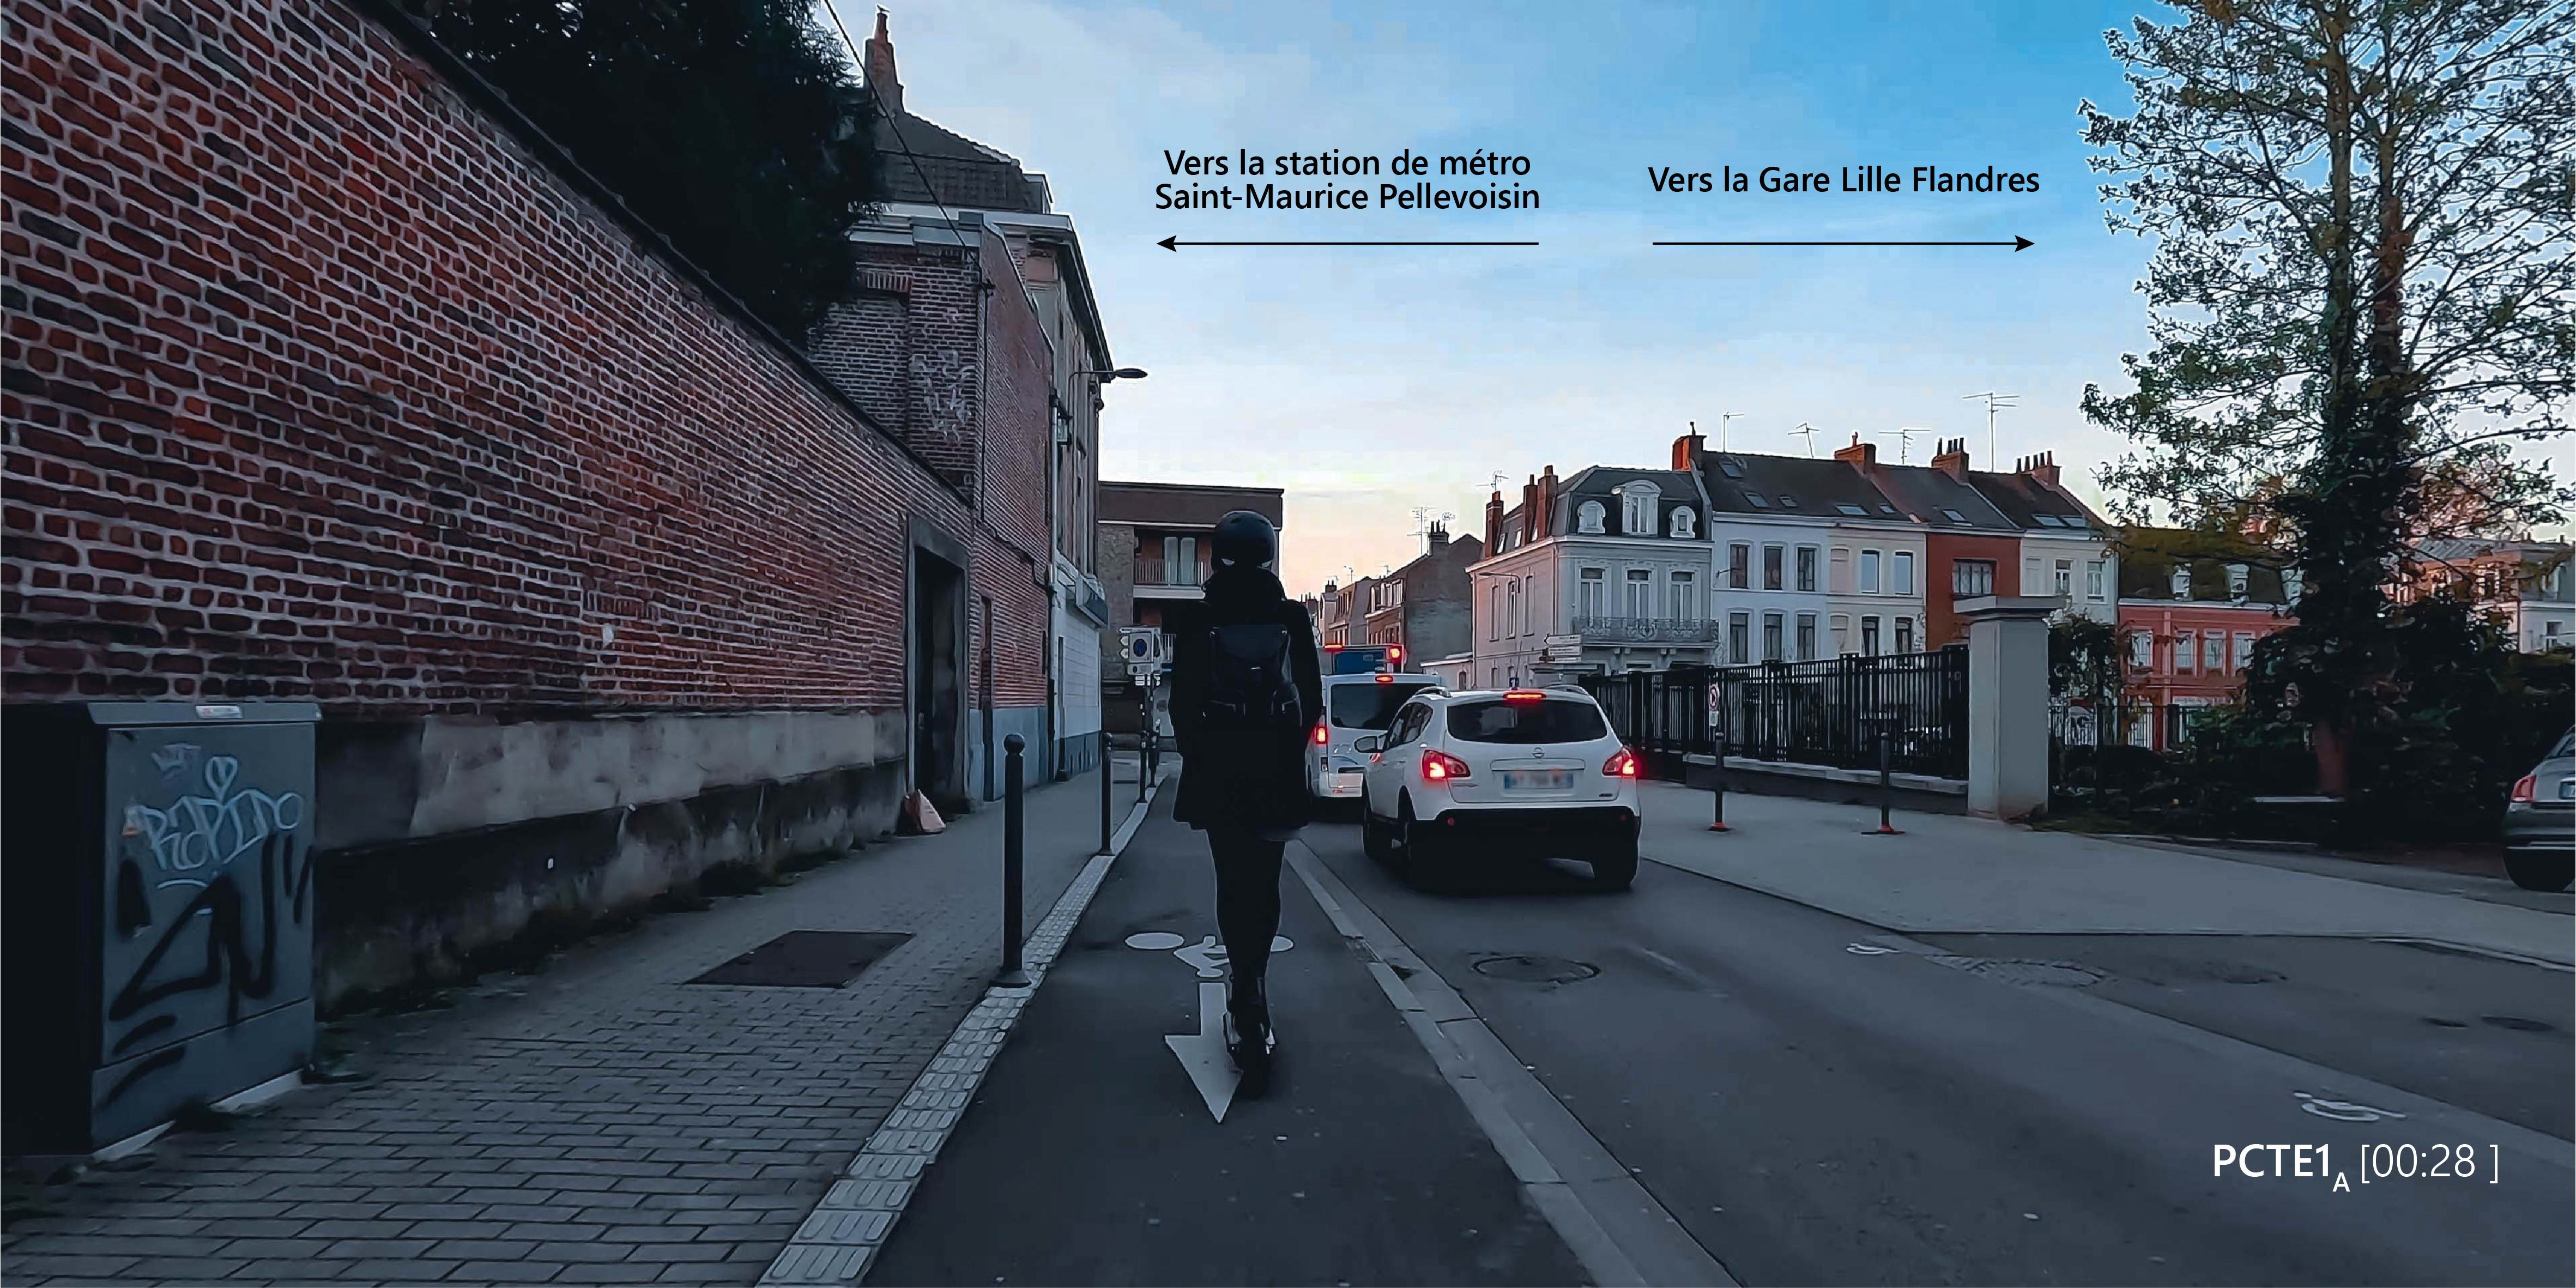
\includegraphics[width=0.75\columnwidth]{src/Figures/Annexes/Extrait_Video_PCTE1_Access_1.jpg}}
        \vspace{5pt}
        \begin{flushright}\scriptsize{
        Author: \textcolor{blue}{Dylan Moinse (2022)}
        }\end{flushright}
    \end{figure}

    % PCTE1 Photo Access 2
    \begin{figure}[h!]\vspace*{4pt}
        \caption*{Excerpt No. 2 from the video during the access segment (\(PCTE^{A}_{1}\))}
        \centerline{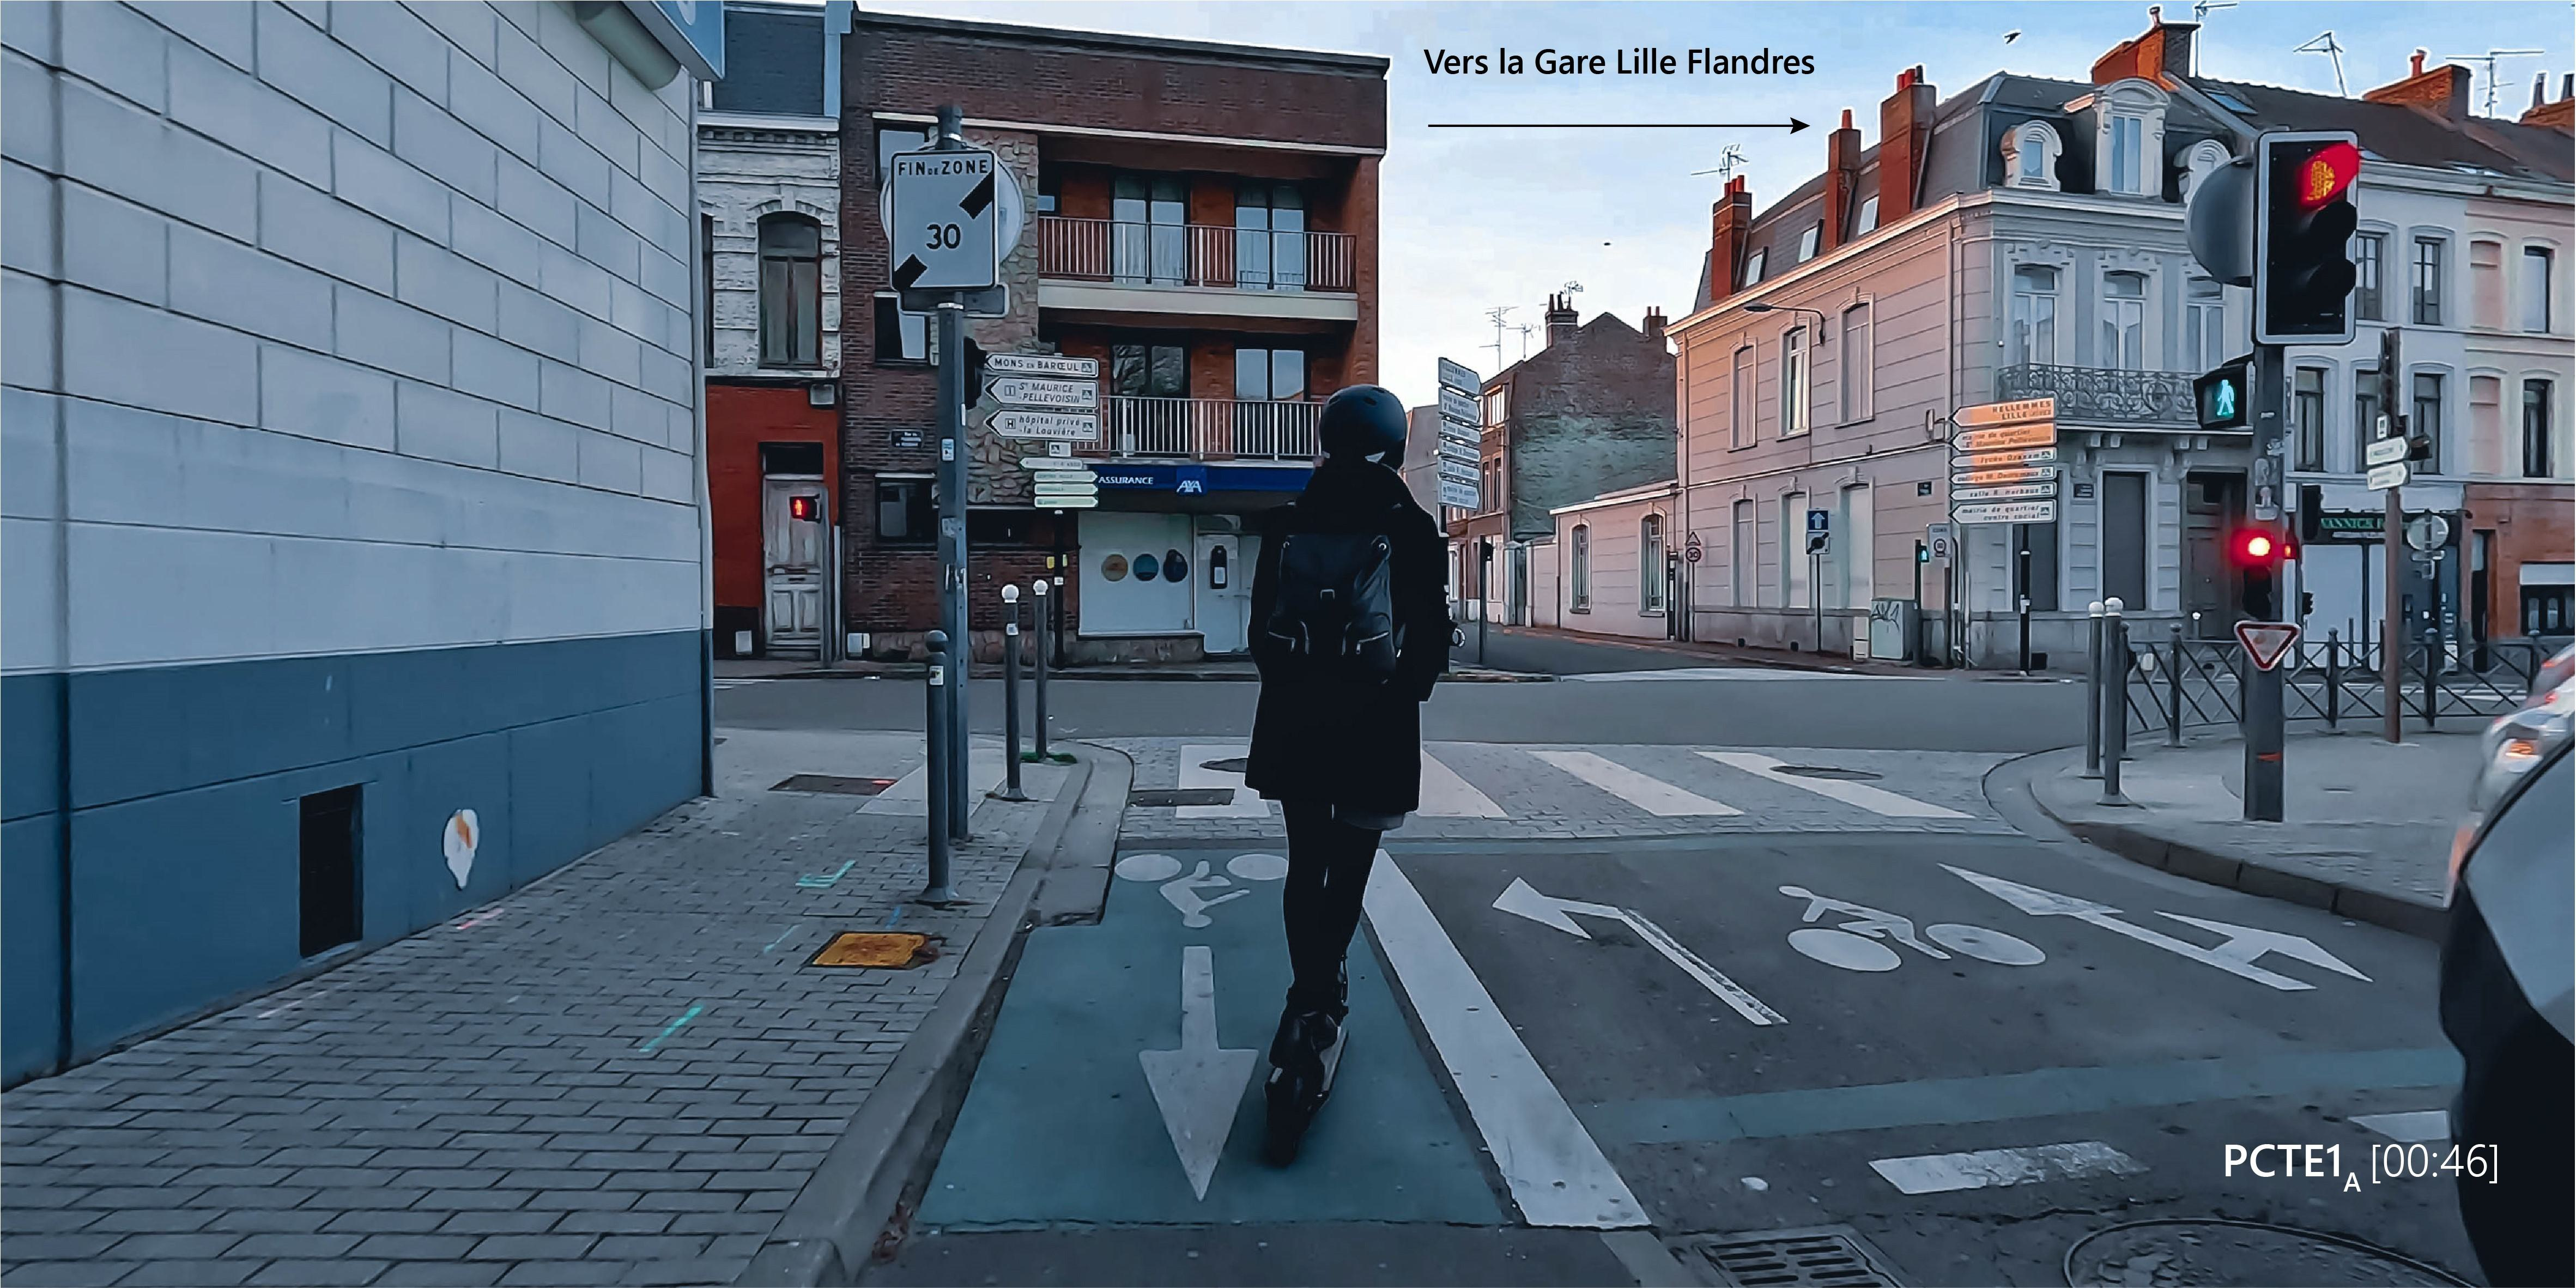
\includegraphics[width=0.75\columnwidth]{src/Figures/Annexes/Extrait_Video_PCTE1_Access_2.jpg}}
        \vspace{5pt}
        \begin{flushright}\scriptsize{
        Author: \textcolor{blue}{Dylan Moinse (2022)}
        }\end{flushright}
    \end{figure}

    % PCTE1 Photo Access 3
    \begin{figure}[h!]\vspace*{4pt}
        \caption*{Excerpt No. 3 from the video during the access segment (\(PCTE^{A}_{1}\))}
        \centerline{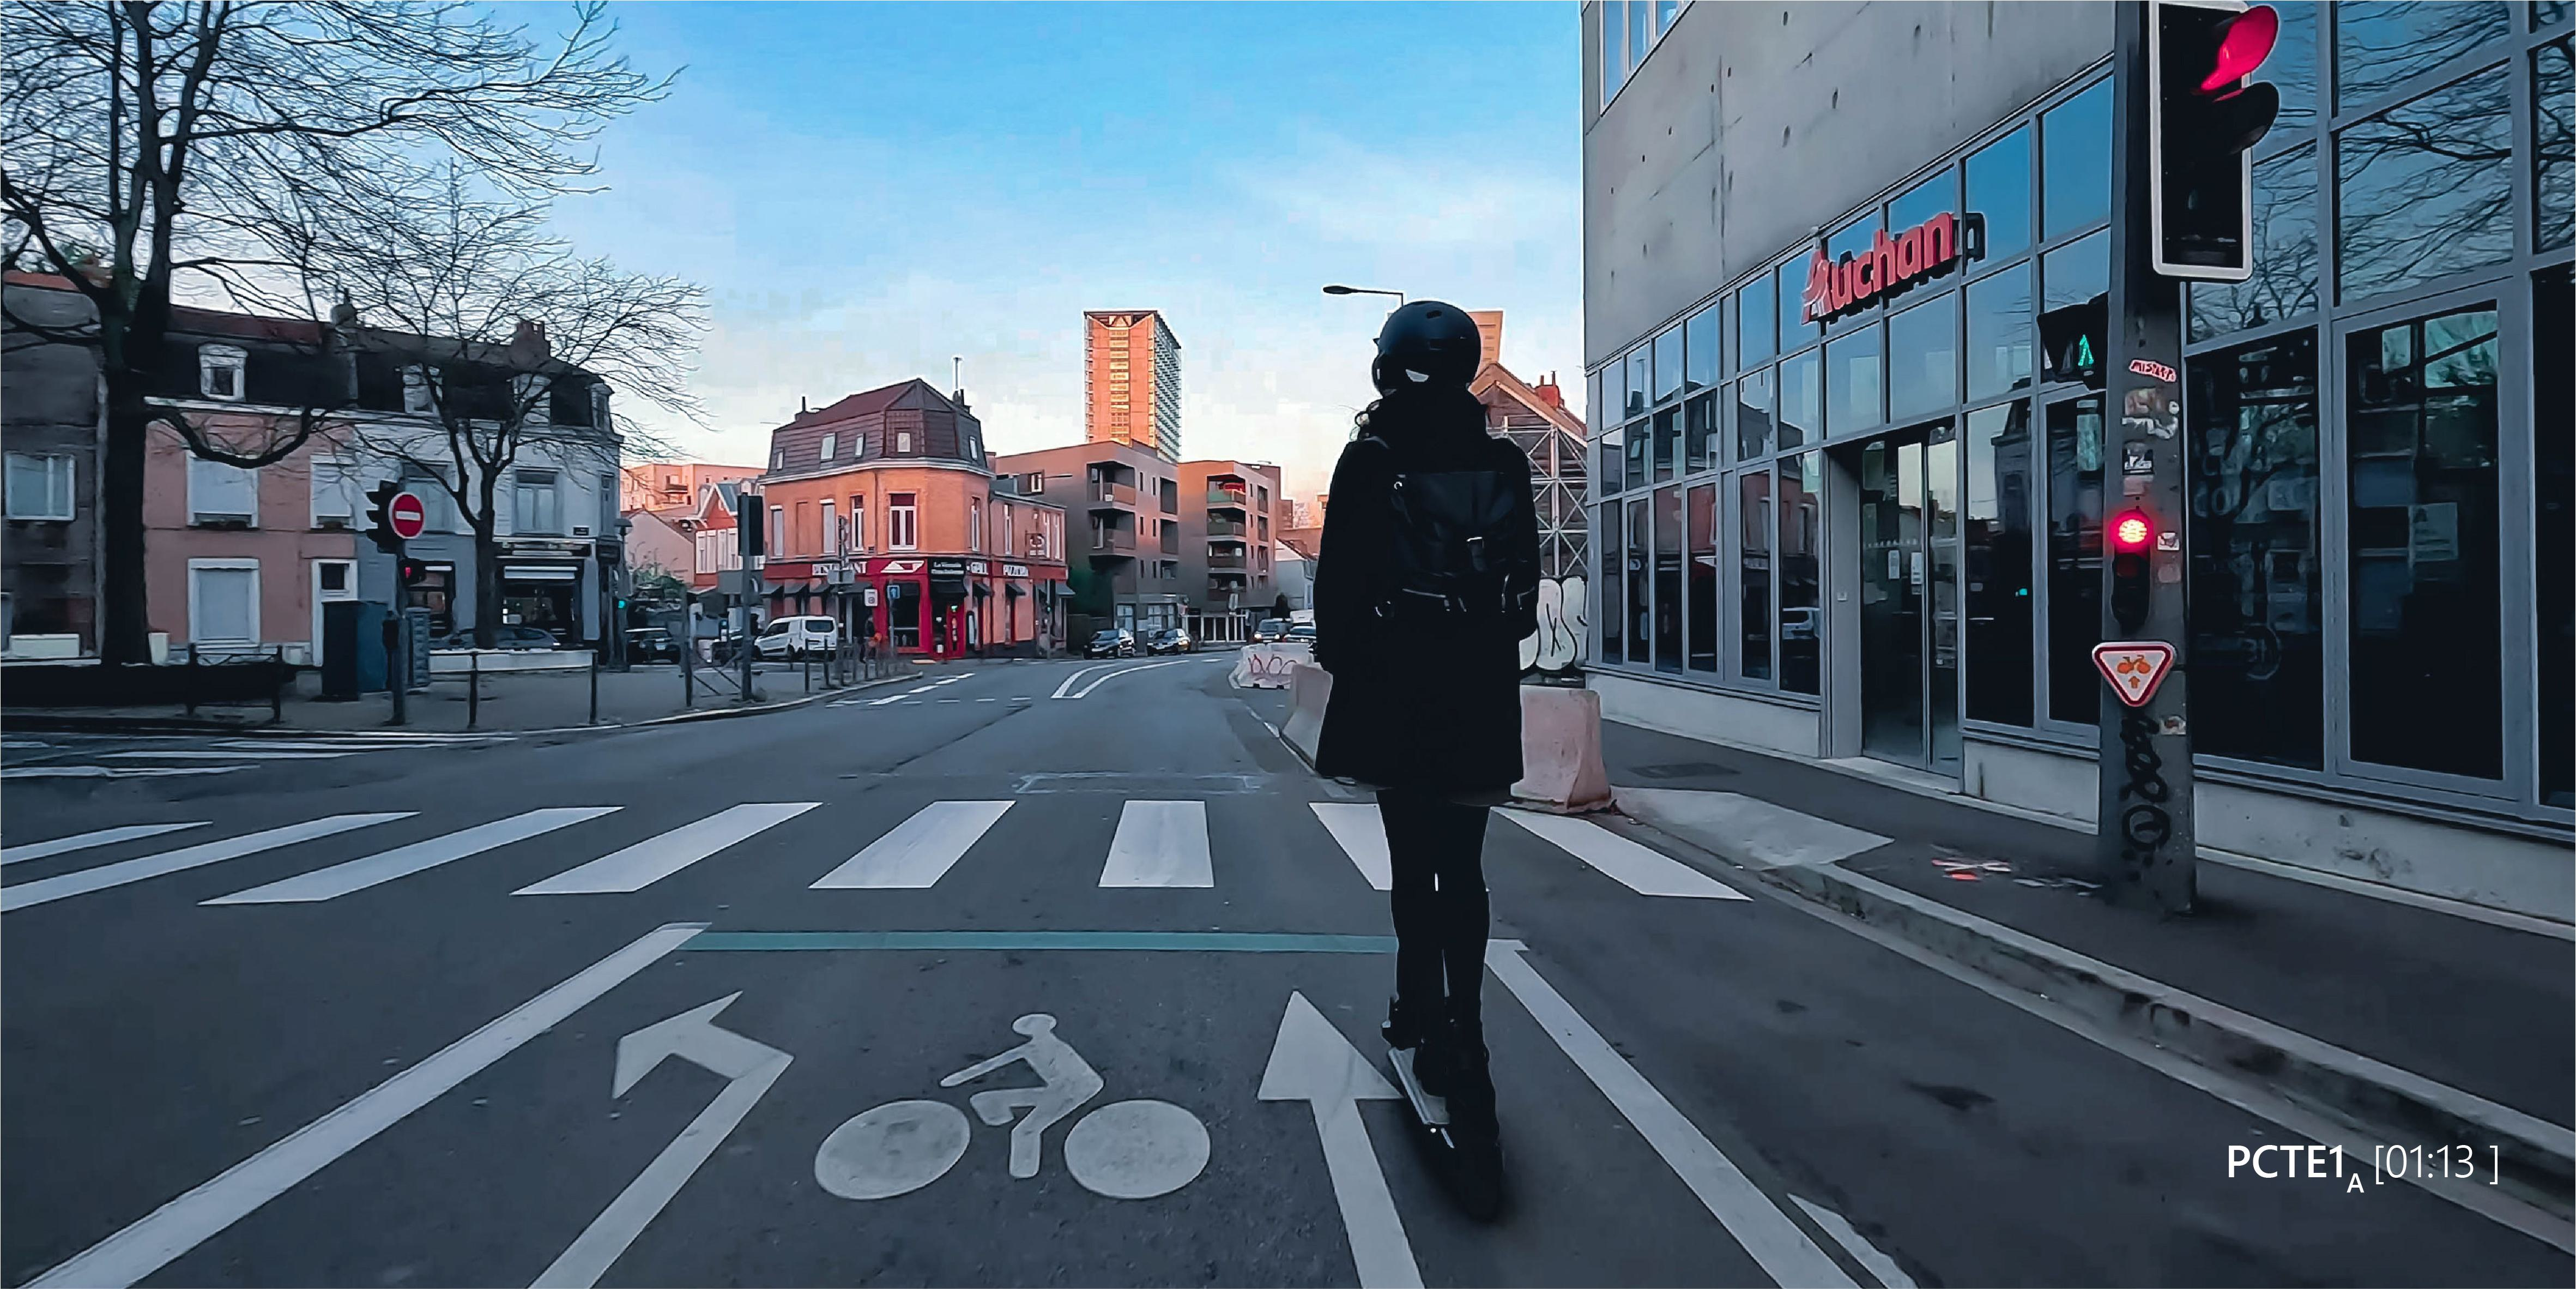
\includegraphics[width=0.75\columnwidth]{src/Figures/Annexes/Extrait_Video_PCTE1_Access_3.jpg}}
        \vspace{5pt}
        \begin{flushright}\scriptsize{
        Author: \textcolor{blue}{Dylan Moinse (2022)}
        }\end{flushright}
    \end{figure}

    % PCTE1 Photo Access 4
    \begin{figure}[h!]\vspace*{4pt}
        \caption*{Excerpt No. 4 from the video during the access segment (\(PCTE^{A}_{1}\))}
        \centerline{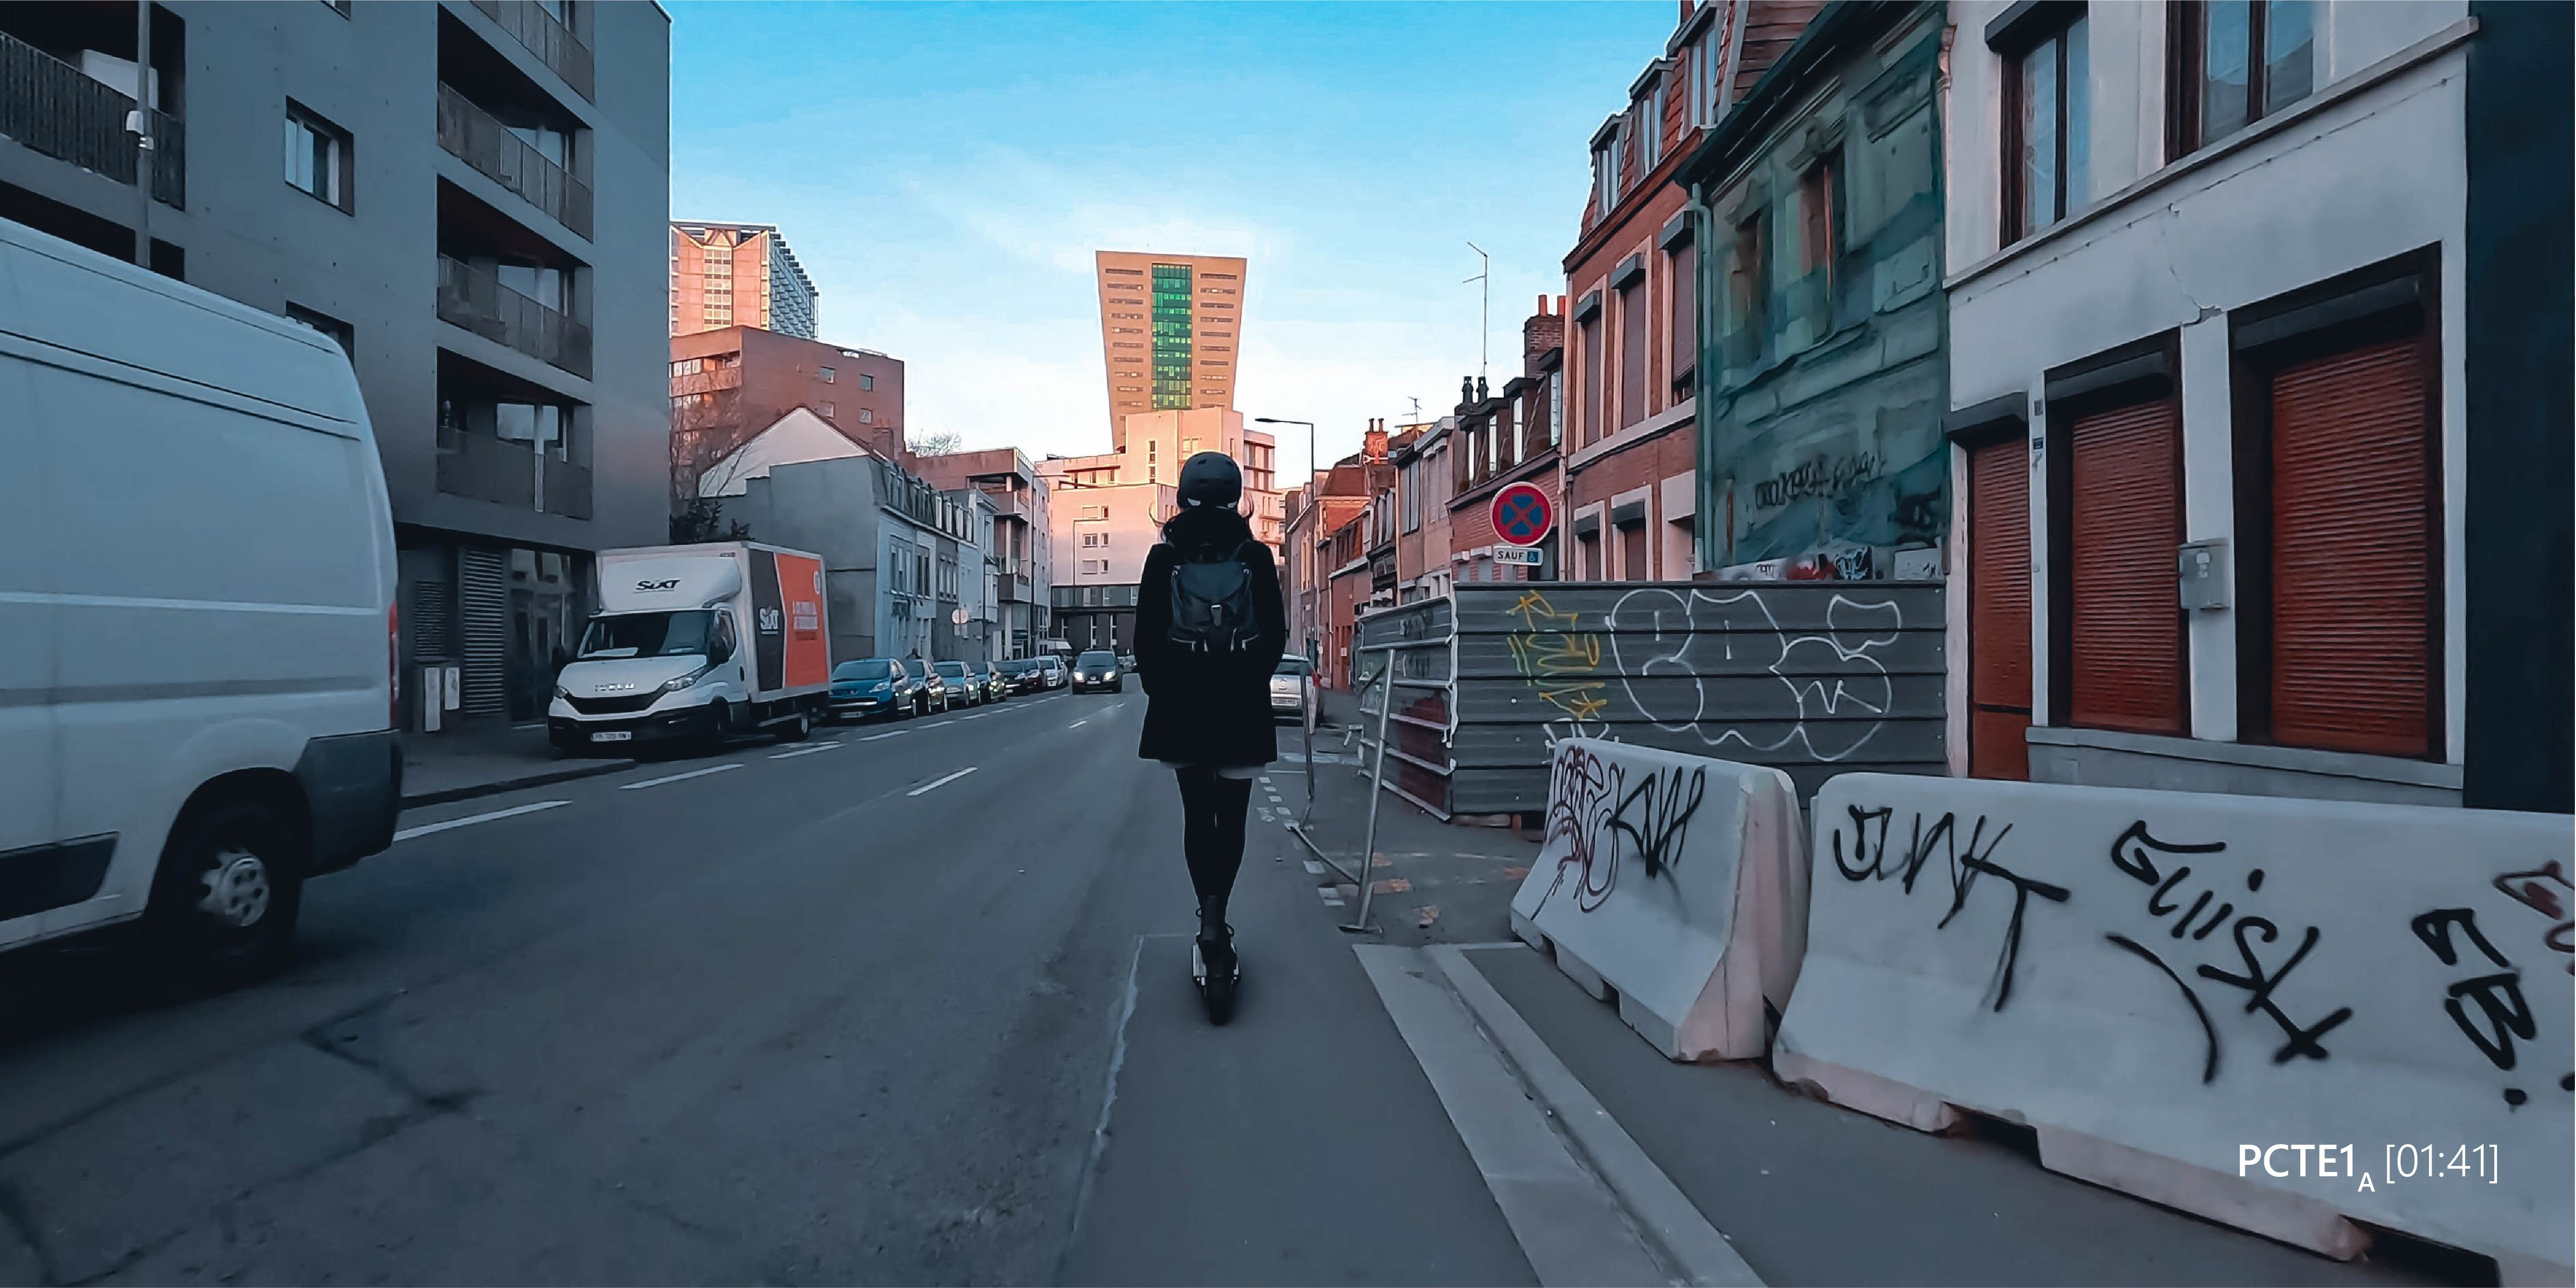
\includegraphics[width=0.75\columnwidth]{src/Figures/Annexes/Extrait_Video_PCTE1_Access_4.jpg}}
        \vspace{5pt}
        \begin{flushright}\scriptsize{
        Author: \textcolor{blue}{Dylan Moinse (2022)}
        }\end{flushright}
    \end{figure}

    % PCTE1 Photo Access 5
    \begin{figure}[h!]\vspace*{4pt}
        \caption*{Excerpt No. 5 from the video during the access segment (\(PCTE^{A}_{1}\))}
        \centerline{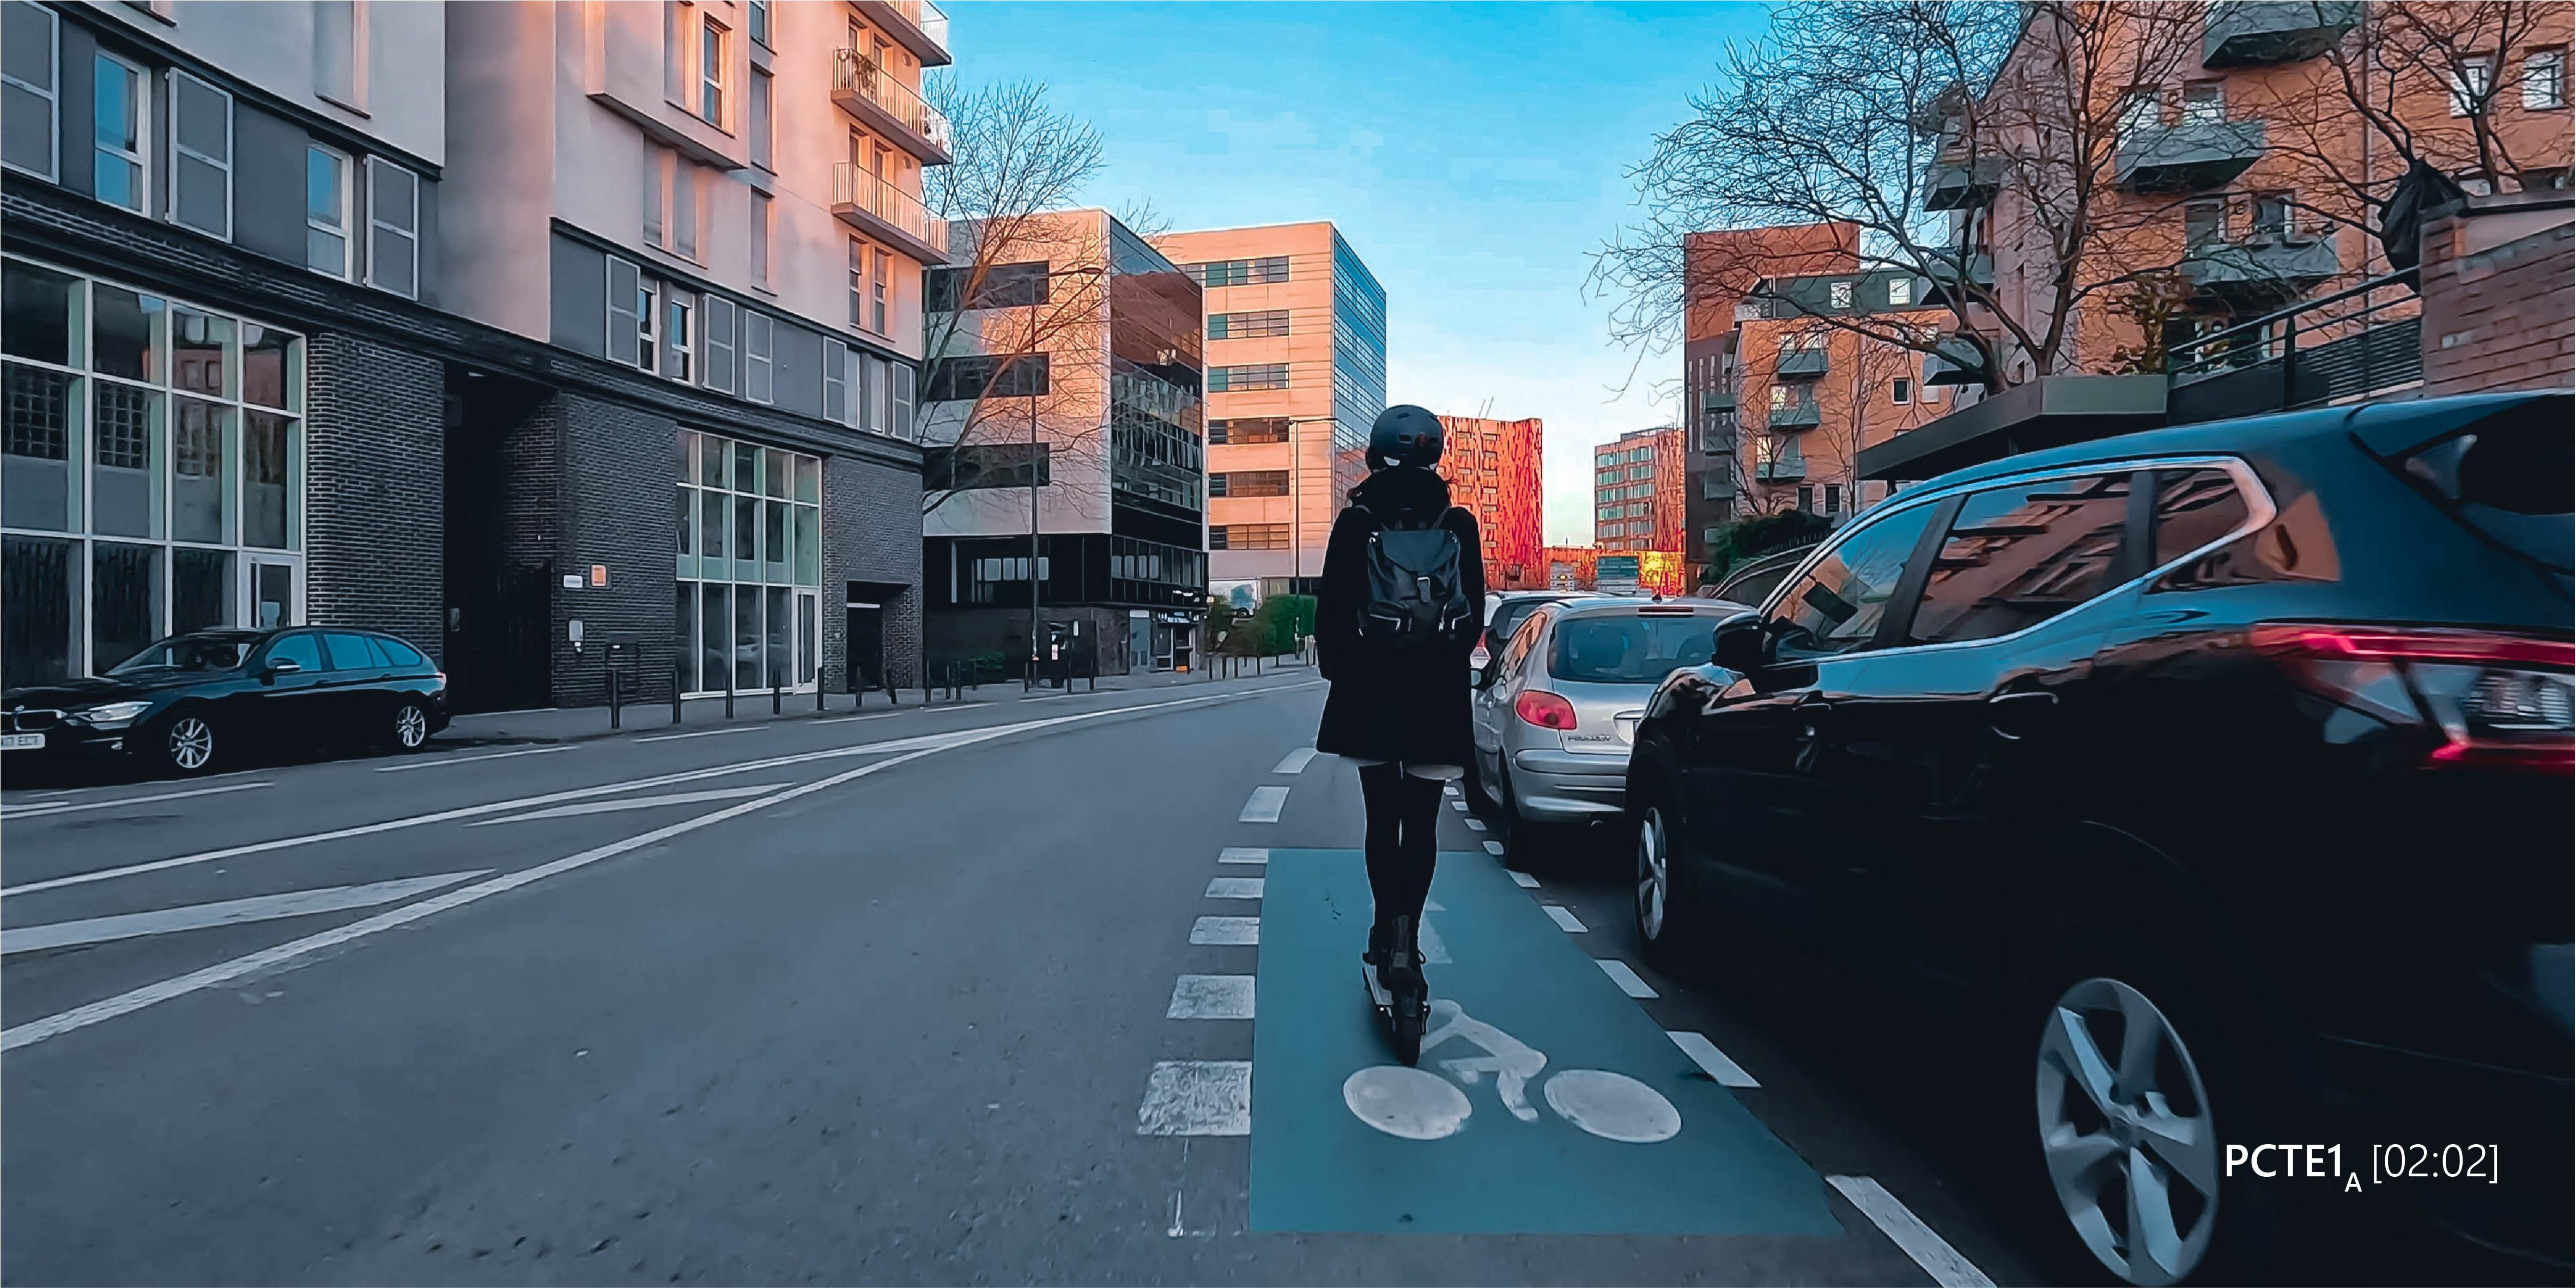
\includegraphics[width=0.75\columnwidth]{src/Figures/Annexes/Extrait_Video_PCTE1_Access_5.jpg}}
        \vspace{5pt}
        \begin{flushright}\scriptsize{
        Author: \textcolor{blue}{Dylan Moinse (2022)}
        }\end{flushright}
    \end{figure}

    % PCTE1 Photo Access 6
    \begin{figure}[h!]\vspace*{4pt}
        \caption*{Excerpt No. 6 from the video during the access segment (\(PCTE^{A}_{1}\))}
        \centerline{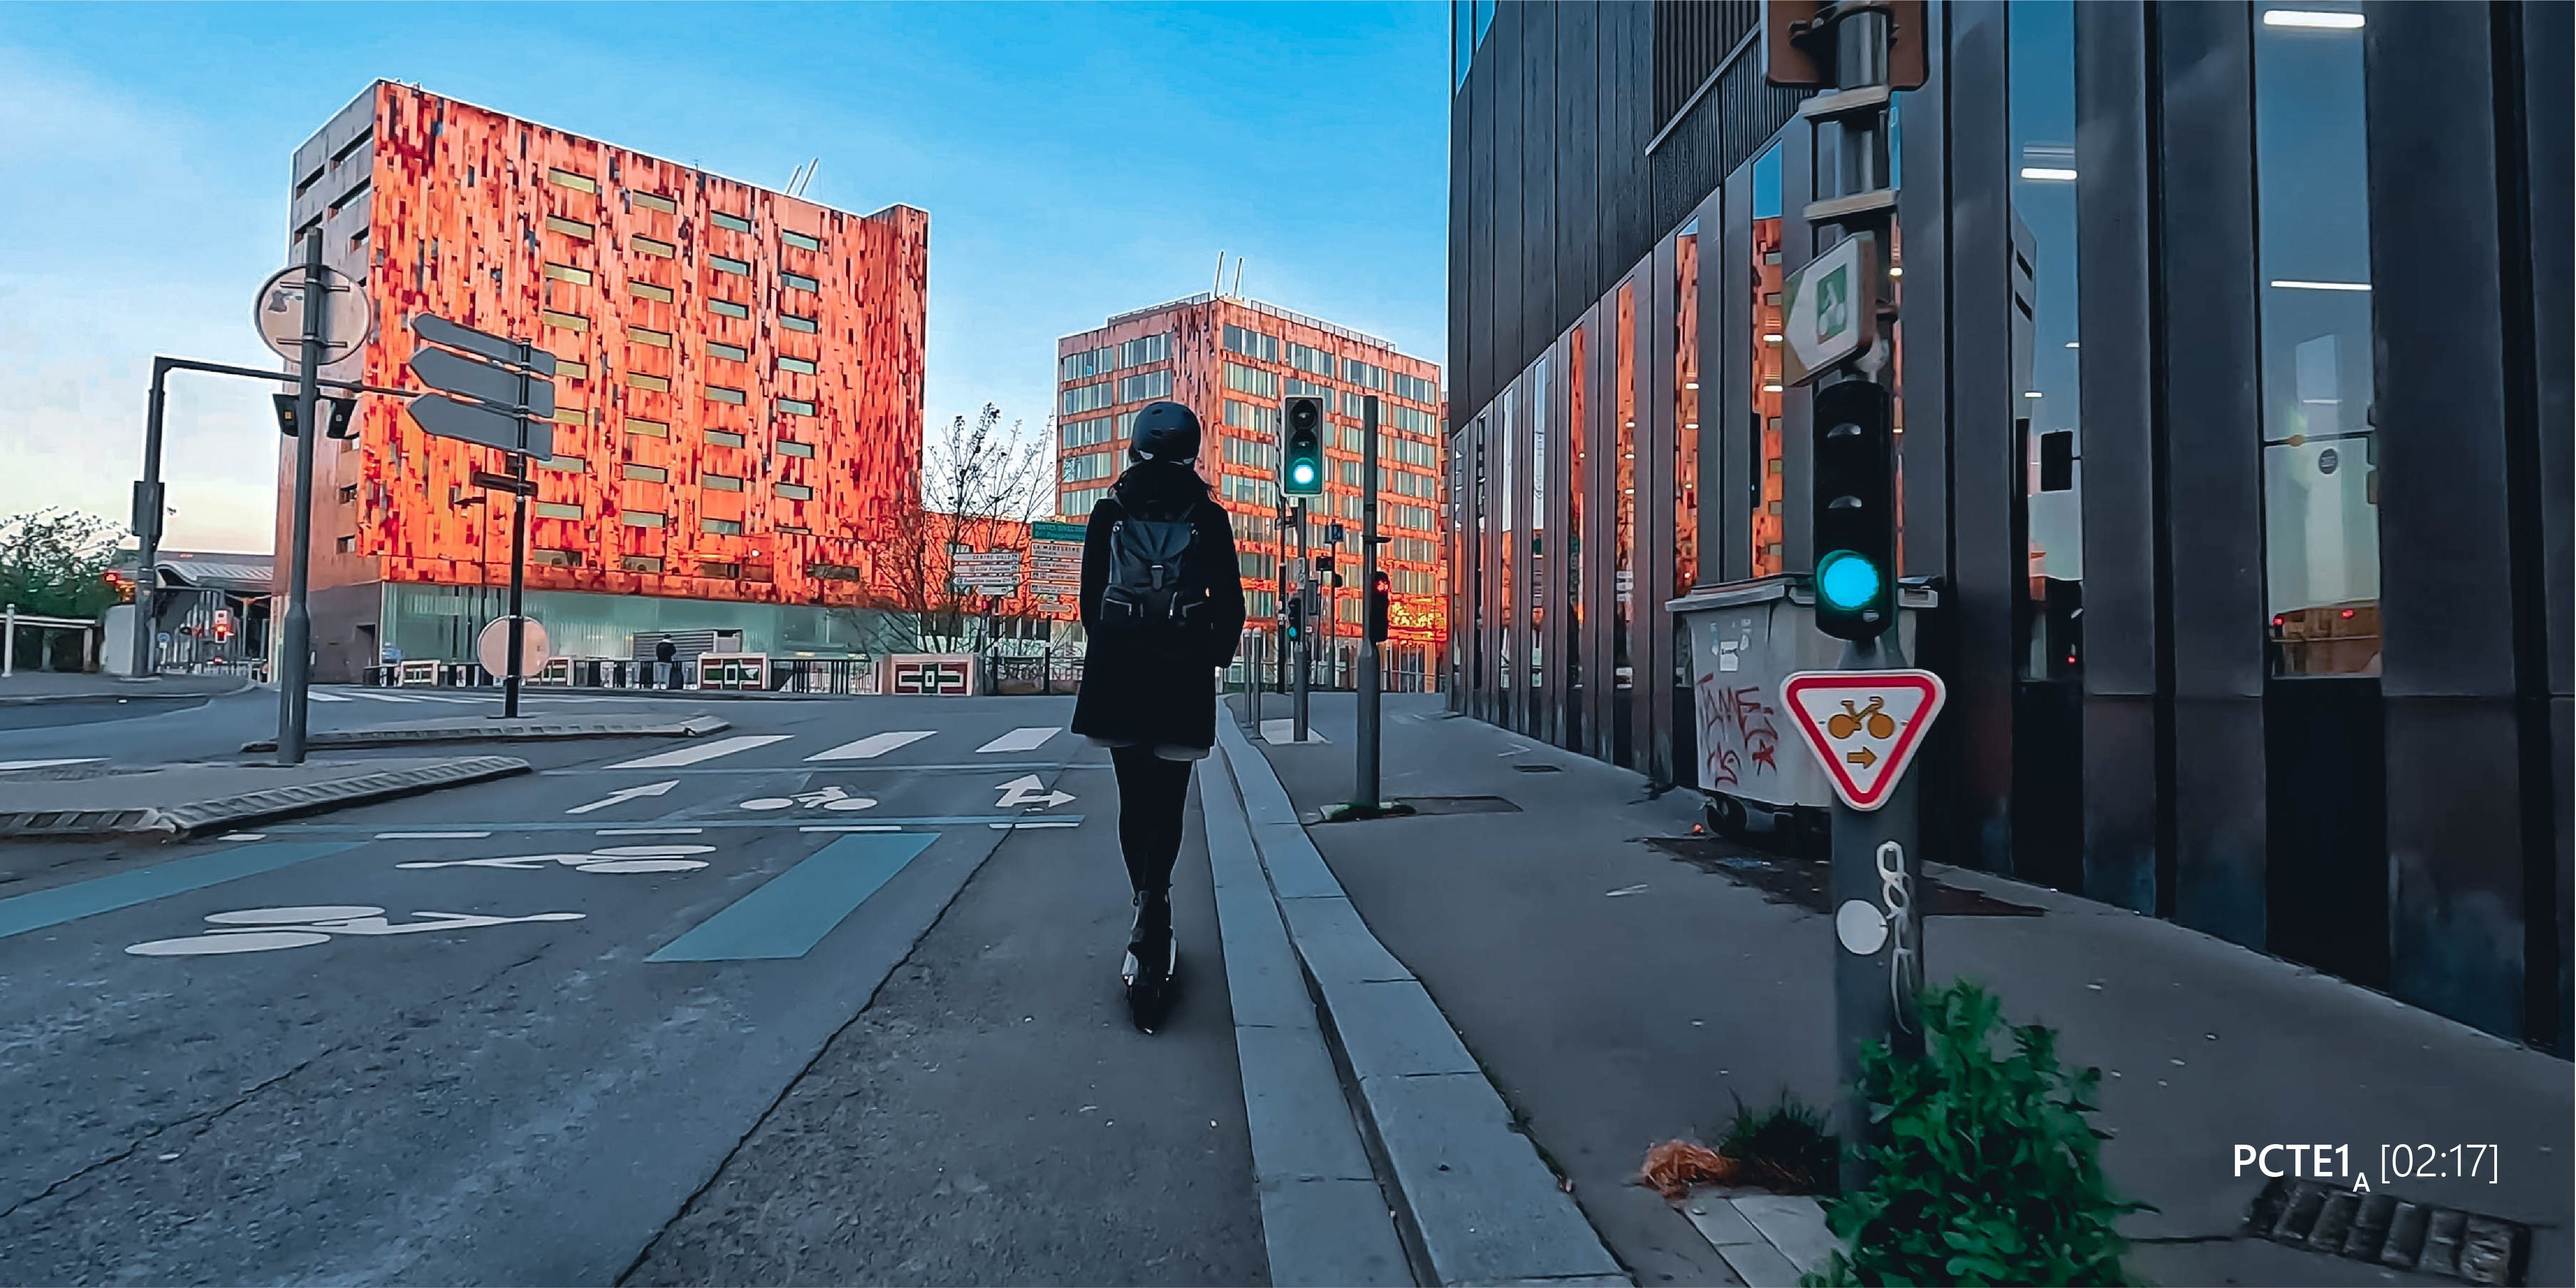
\includegraphics[width=0.75\columnwidth]{src/Figures/Annexes/Extrait_Video_PCTE1_Access_6.jpg}}
        \vspace{5pt}
        \begin{flushright}\scriptsize{
        Author: \textcolor{blue}{Dylan Moinse (2022)}
        }\end{flushright}
    \end{figure}

    % PCTE1 Photo Access 7
    \begin{figure}[h!]\vspace*{4pt}
        \caption*{Excerpt No. 7 from the video during the access segment (\(PCTE^{A}_{1}\))}
        \centerline{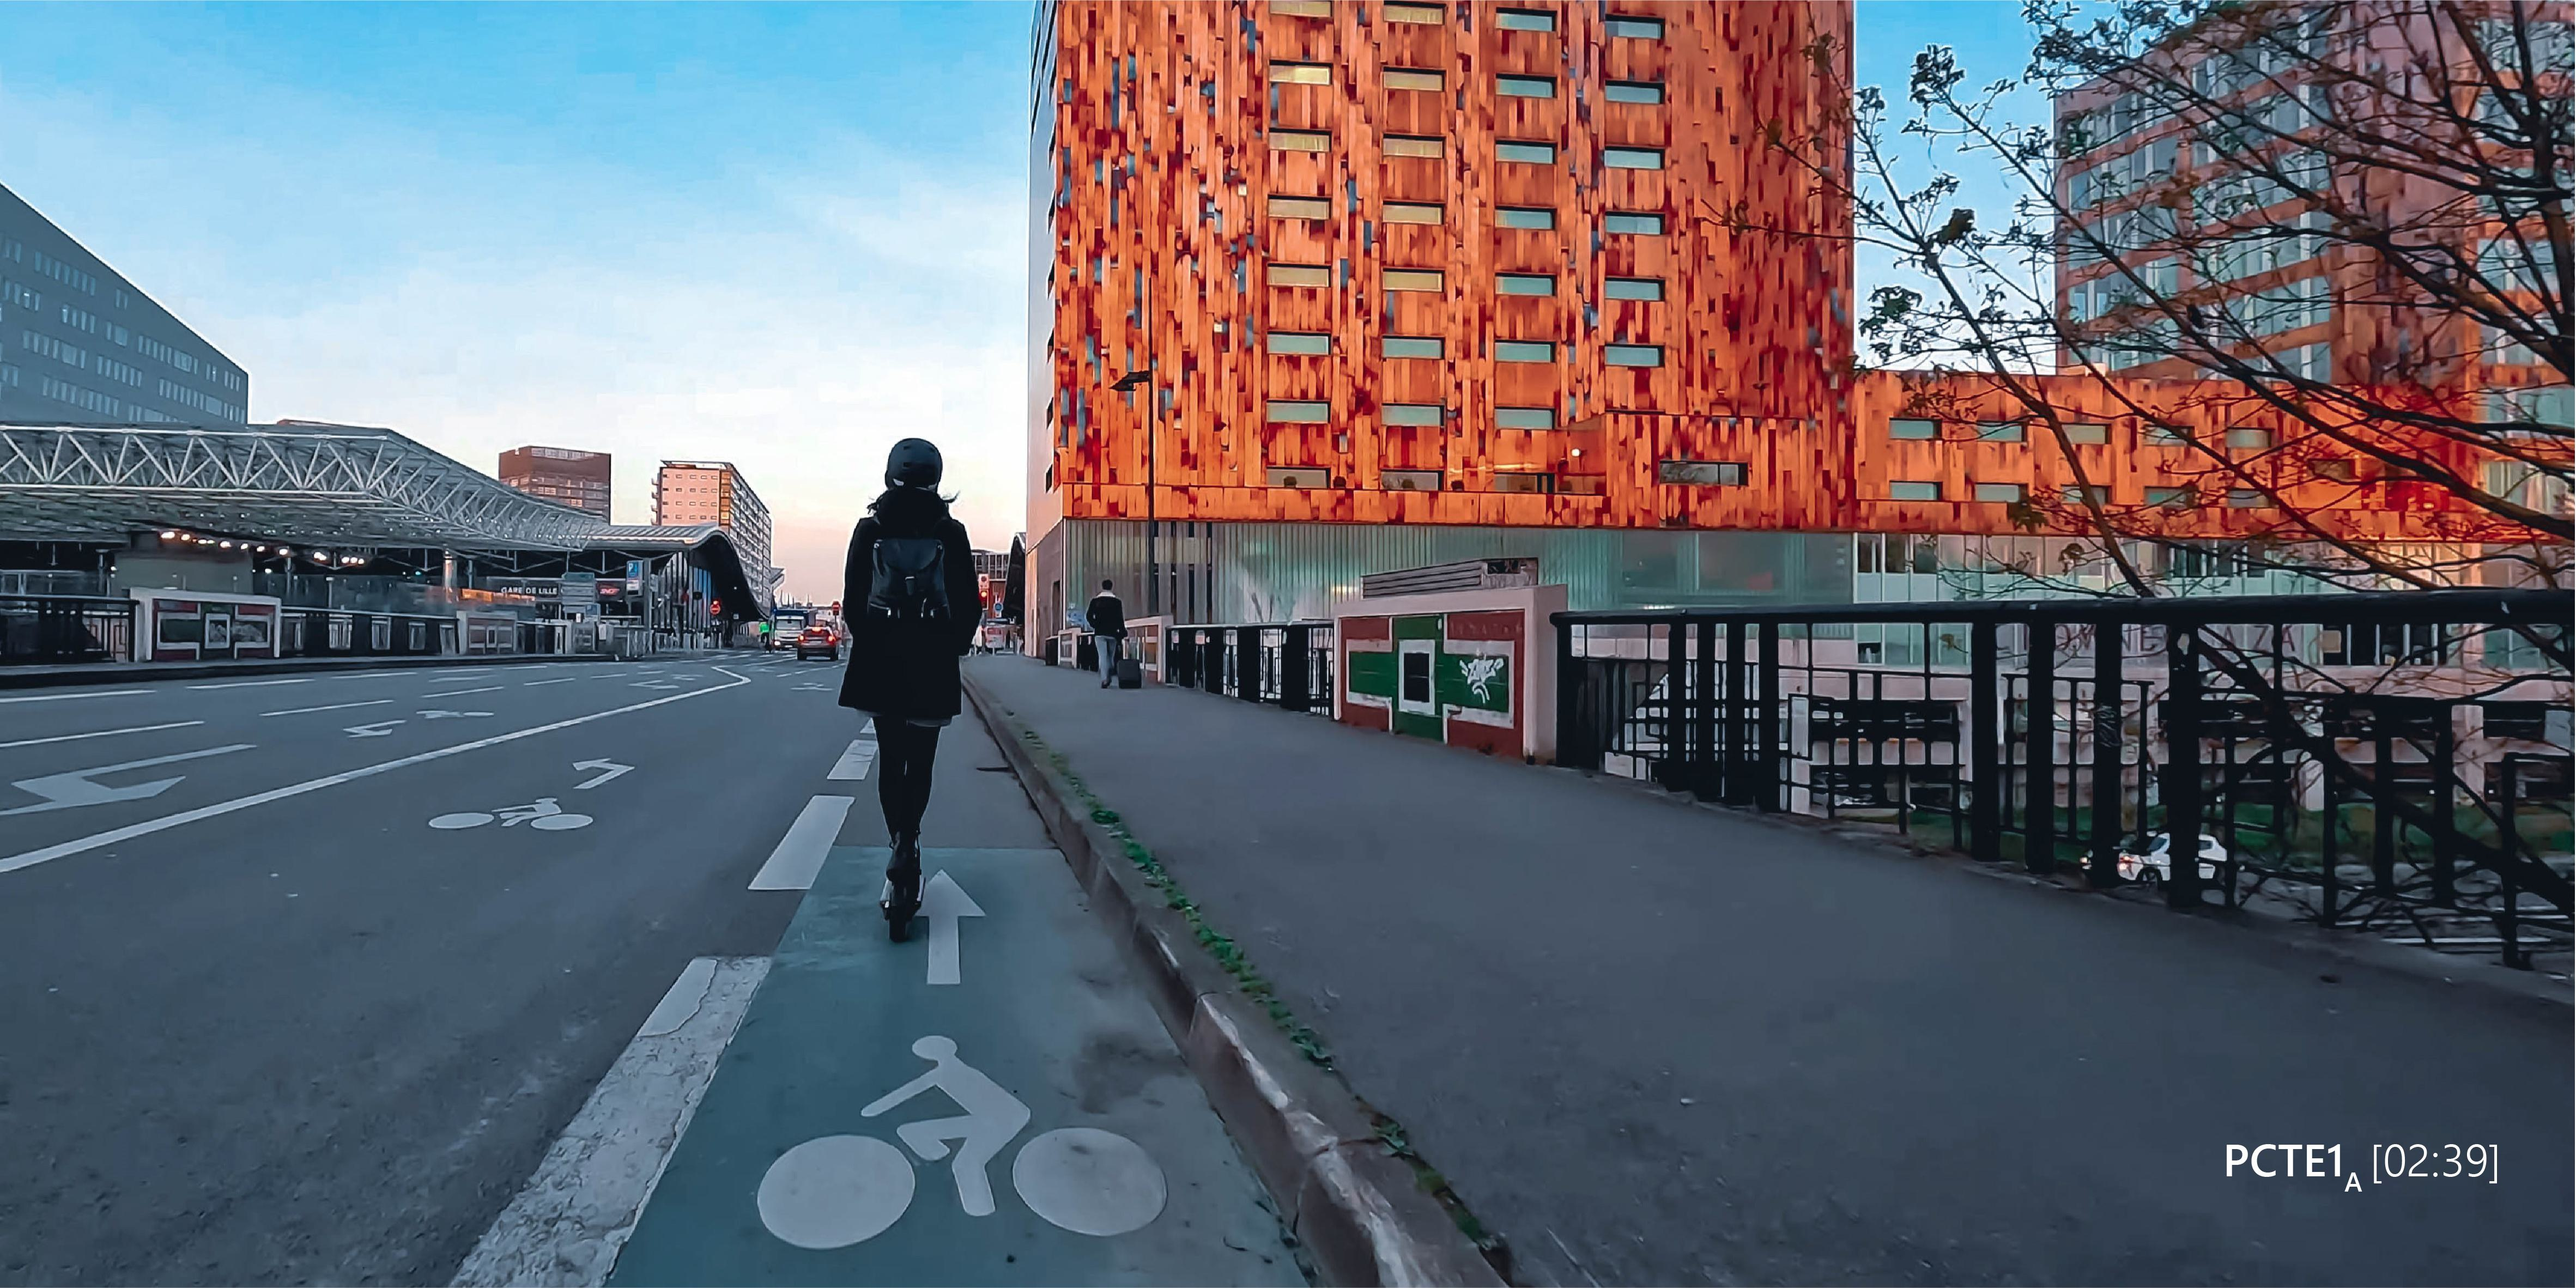
\includegraphics[width=0.75\columnwidth]{src/Figures/Annexes/Extrait_Video_PCTE1_Access_7.jpg}}
        \vspace{5pt}
        \begin{flushright}\scriptsize{
        Author: \textcolor{blue}{Dylan Moinse (2022)}
        }\end{flushright}
    \end{figure}

    % PCTE1 Photo Access 8
    \begin{figure}[h!]\vspace*{4pt}
        \caption*{Excerpt No. 8 from the video during the access segment (\(PCTE^{A}_{1}\))}
        \centerline{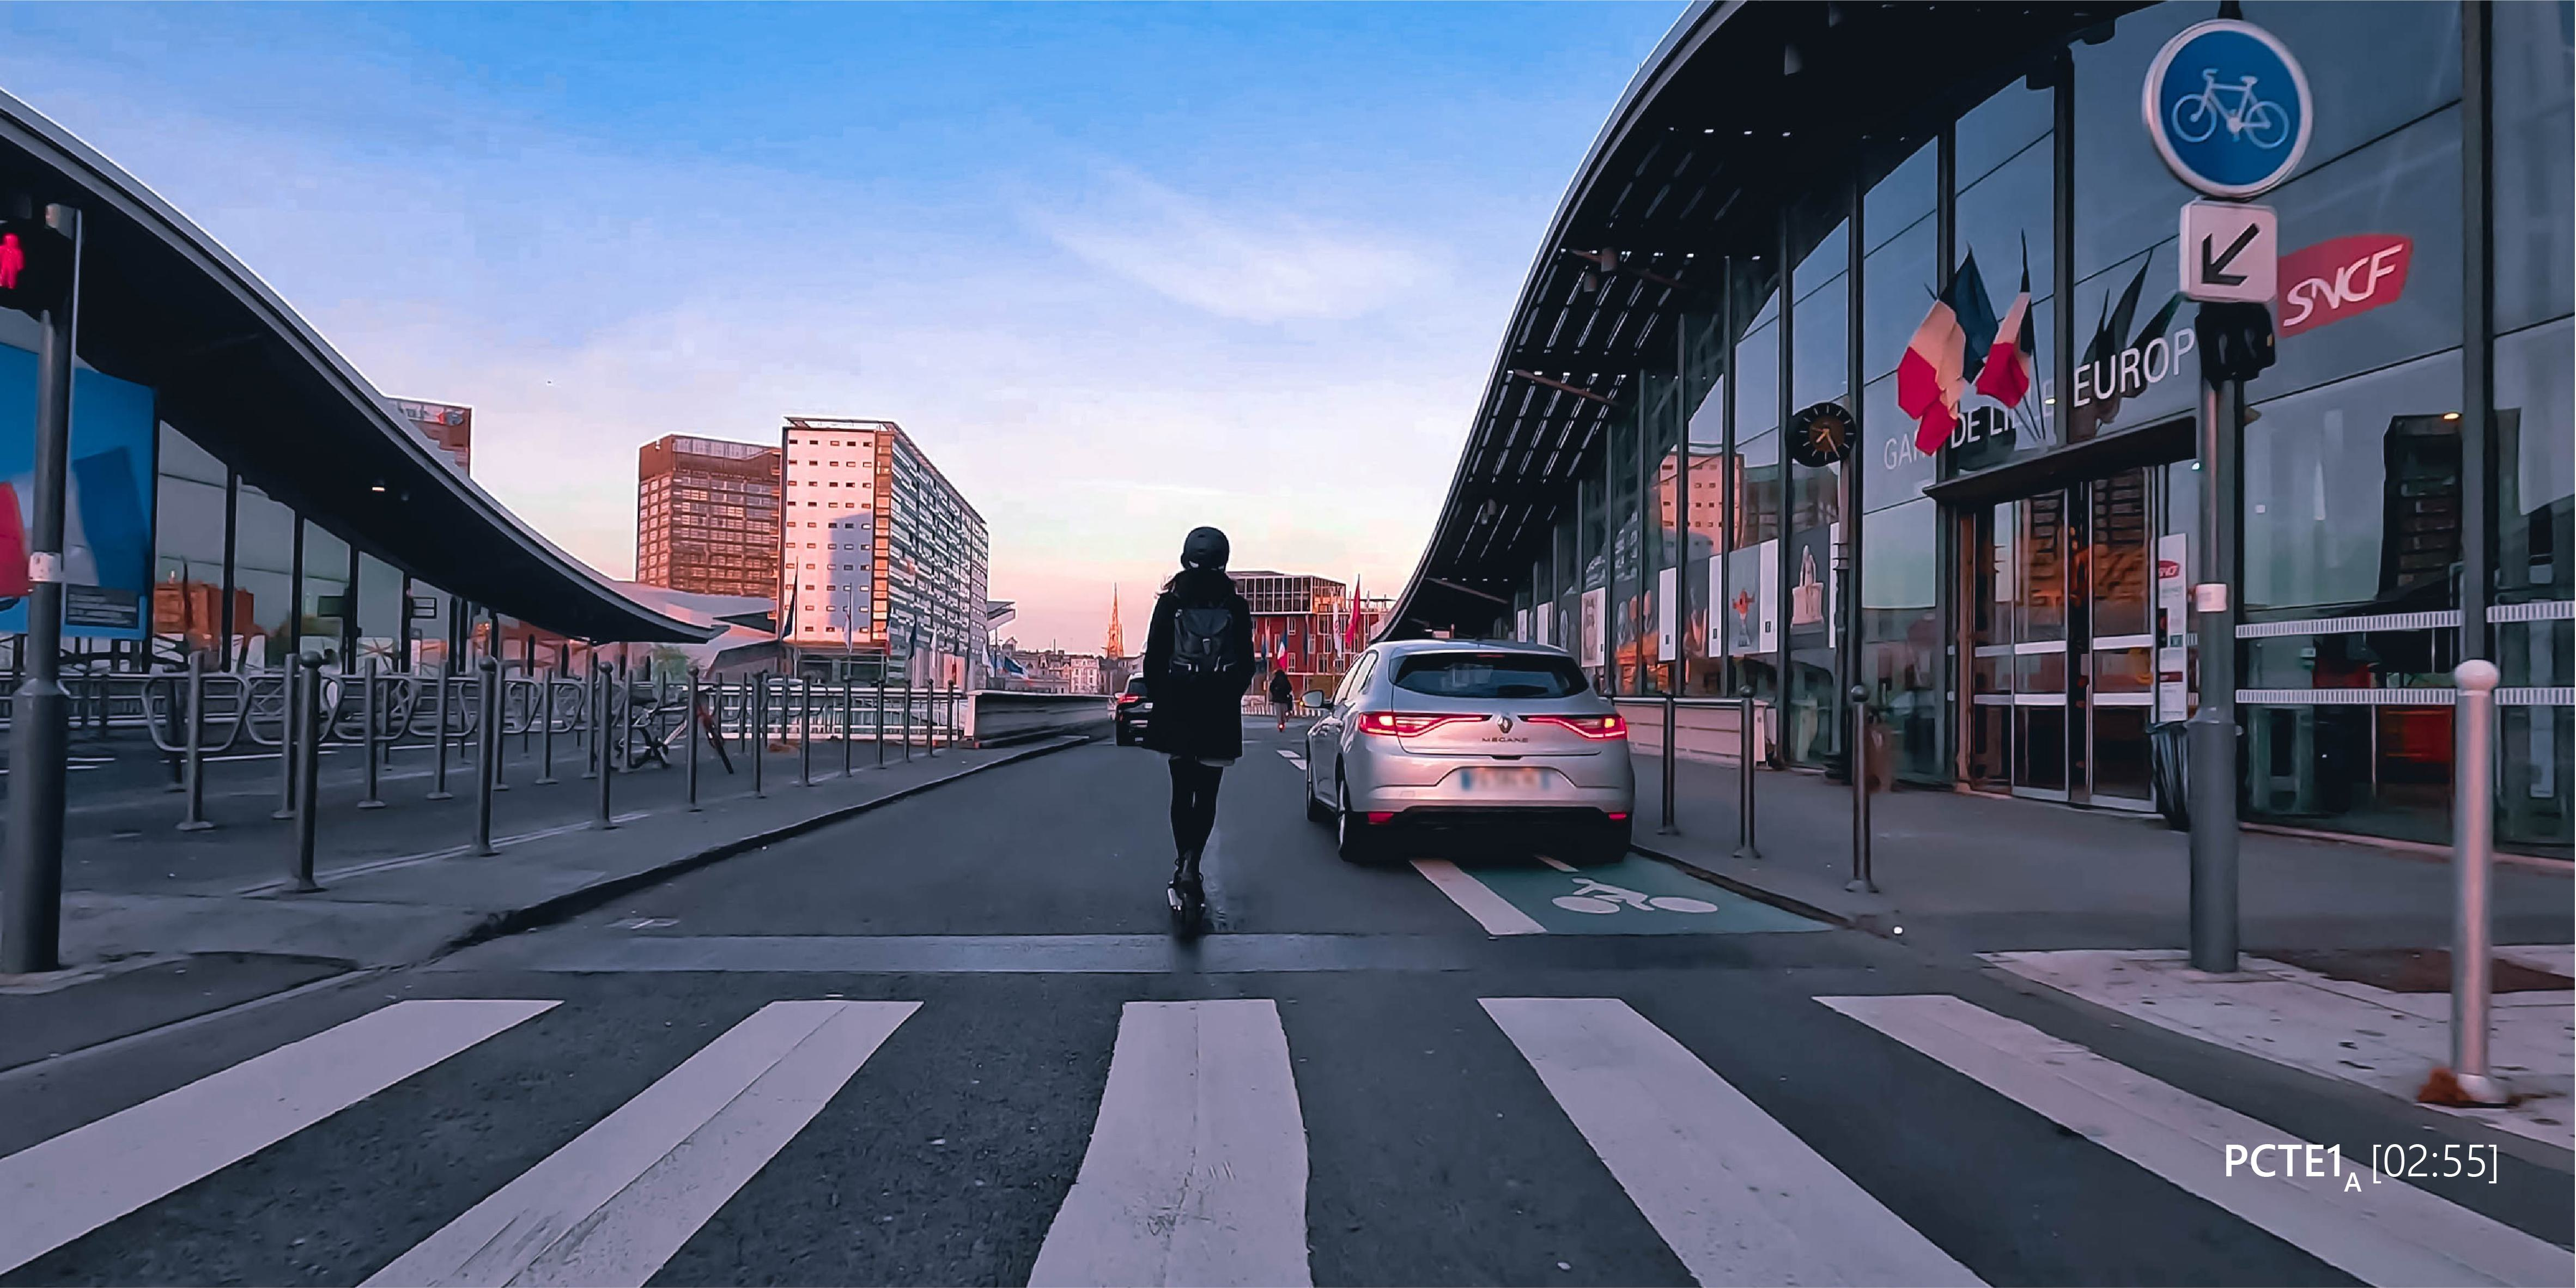
\includegraphics[width=0.75\columnwidth]{src/Figures/Annexes/Extrait_Video_PCTE1_Access_8.jpg}}
        \vspace{5pt}
        \begin{flushright}\scriptsize{
        Author: \textcolor{blue}{Dylan Moinse (2022)}
        }\end{flushright}
    \end{figure}

    % PCTE1 Photo Access 9
    \begin{figure}[h!]\vspace*{4pt}
        \caption*{Excerpt No. 9 from the video during the access segment (\(PCTE^{A}_{1}\))}
        \centerline{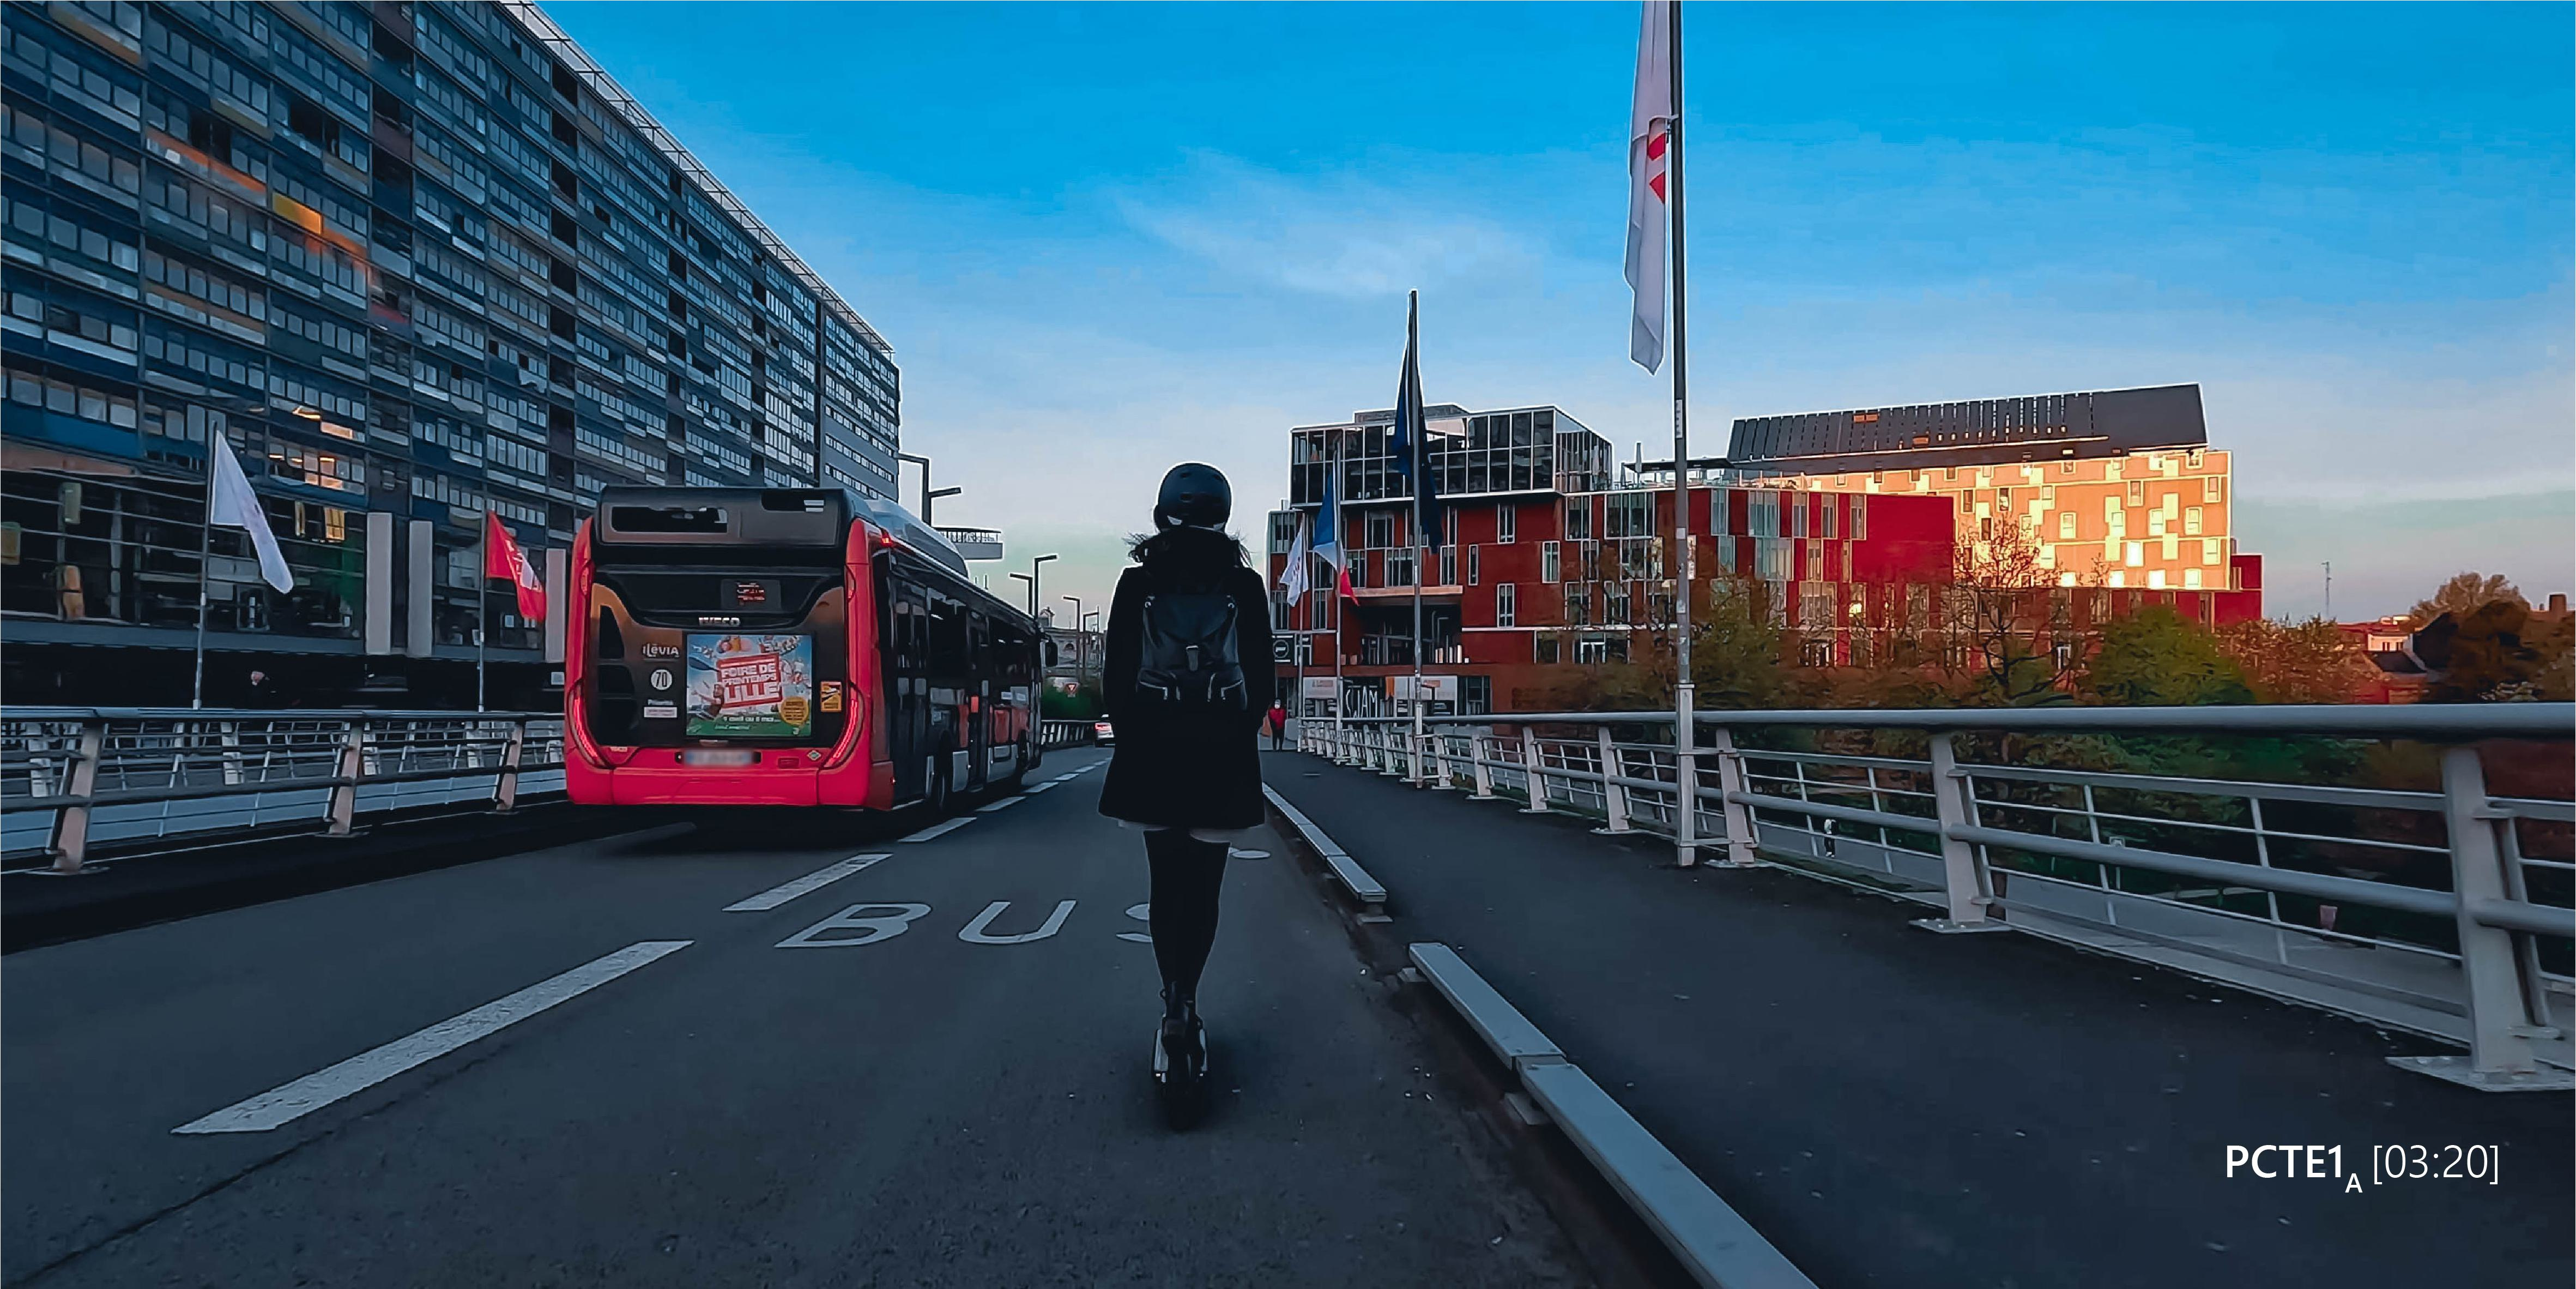
\includegraphics[width=0.75\columnwidth]{src/Figures/Annexes/Extrait_Video_PCTE1_Access_9.jpg}}
        \vspace{5pt}
        \begin{flushright}\scriptsize{
        Author: \textcolor{blue}{Dylan Moinse (2022)}
        }\end{flushright}
    \end{figure}

    % PCTE1 Photo Access 10
    \begin{figure}[h!]\vspace*{4pt}
        \caption*{Excerpt No. 10 from the video during the access segment (\(PCTE^{A}_{1}\))}
        \centerline{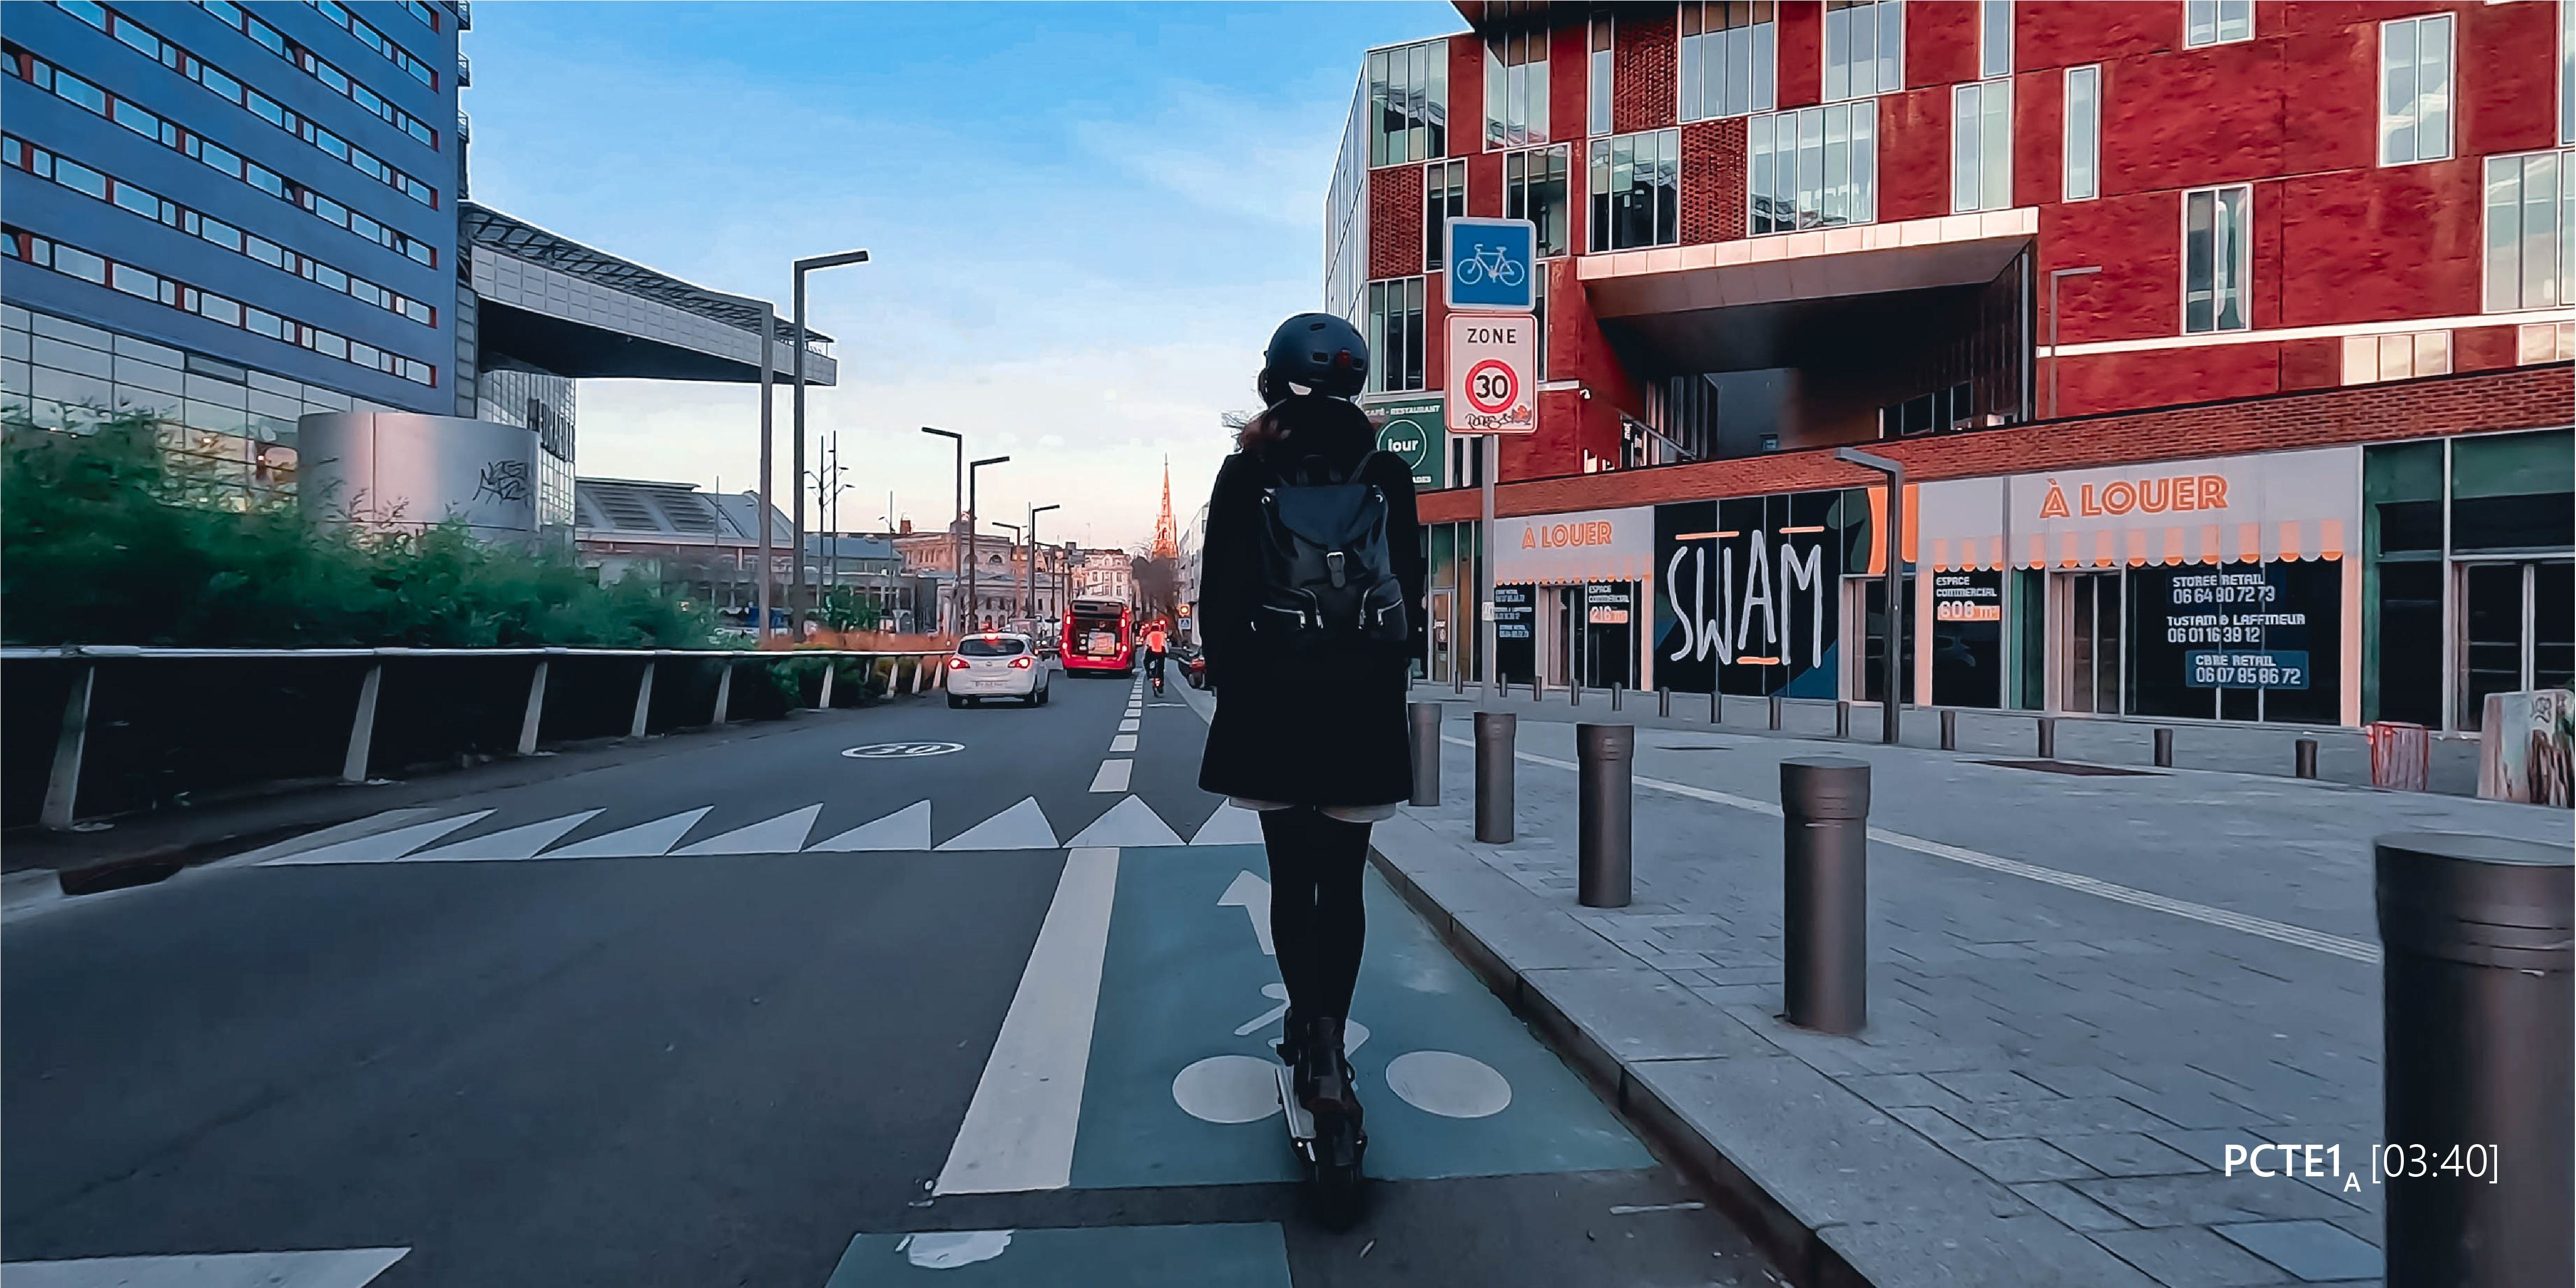
\includegraphics[width=0.75\columnwidth]{src/Figures/Annexes/Extrait_Video_PCTE1_Access_10.jpg}}
        \vspace{5pt}
        \begin{flushright}\scriptsize{
        Author: \textcolor{blue}{Dylan Moinse (2022)}
        }\end{flushright}
    \end{figure}
    
    % PCTE1 Photo Access 11
    \begin{figure}[h!]\vspace*{4pt}
        \caption*{Excerpt No. 11 from the video during the access segment (\(PCTE^{A}_{1}\))}
        \centerline{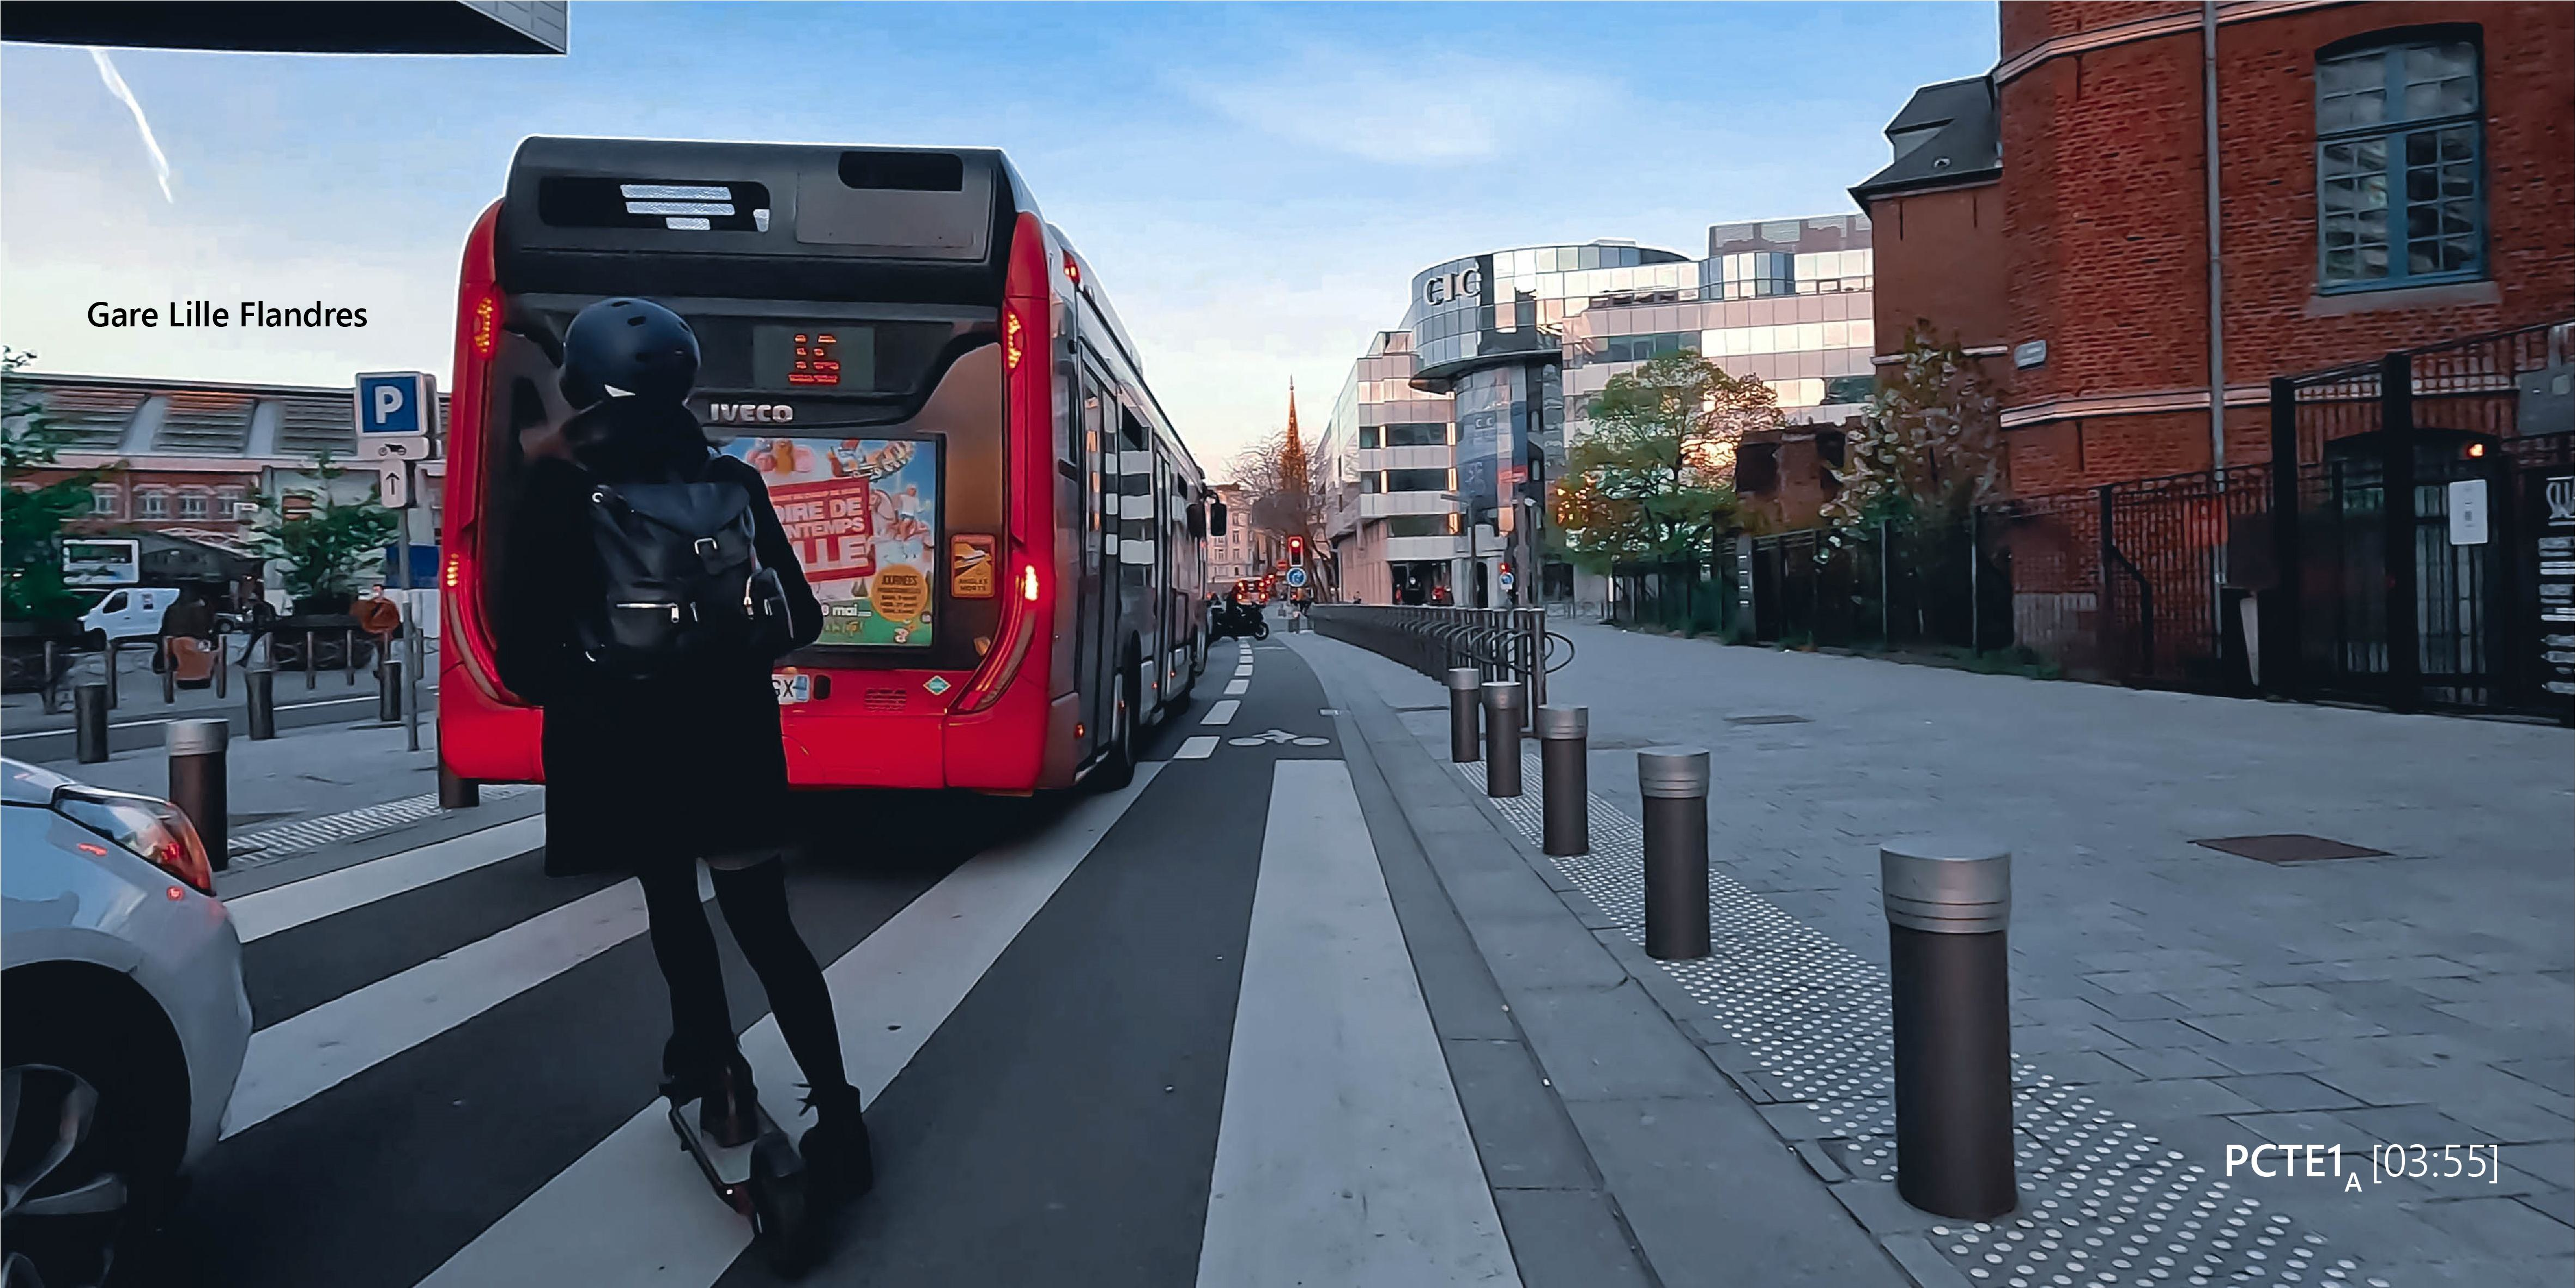
\includegraphics[width=0.75\columnwidth]{src/Figures/Annexes/Extrait_Video_PCTE1_Access_11.jpg}}
        \vspace{5pt}
        \begin{flushright}\scriptsize{
        Author: \textcolor{blue}{Dylan Moinse (2022)}
        }\end{flushright}
    \end{figure}

    % PCTE1 Photo Access 12
    \begin{figure}[h!]\vspace*{4pt}
        \caption*{Excerpt No. 12 from the video during the access segment (\(PCTE^{A}_{1}\))}
        \centerline{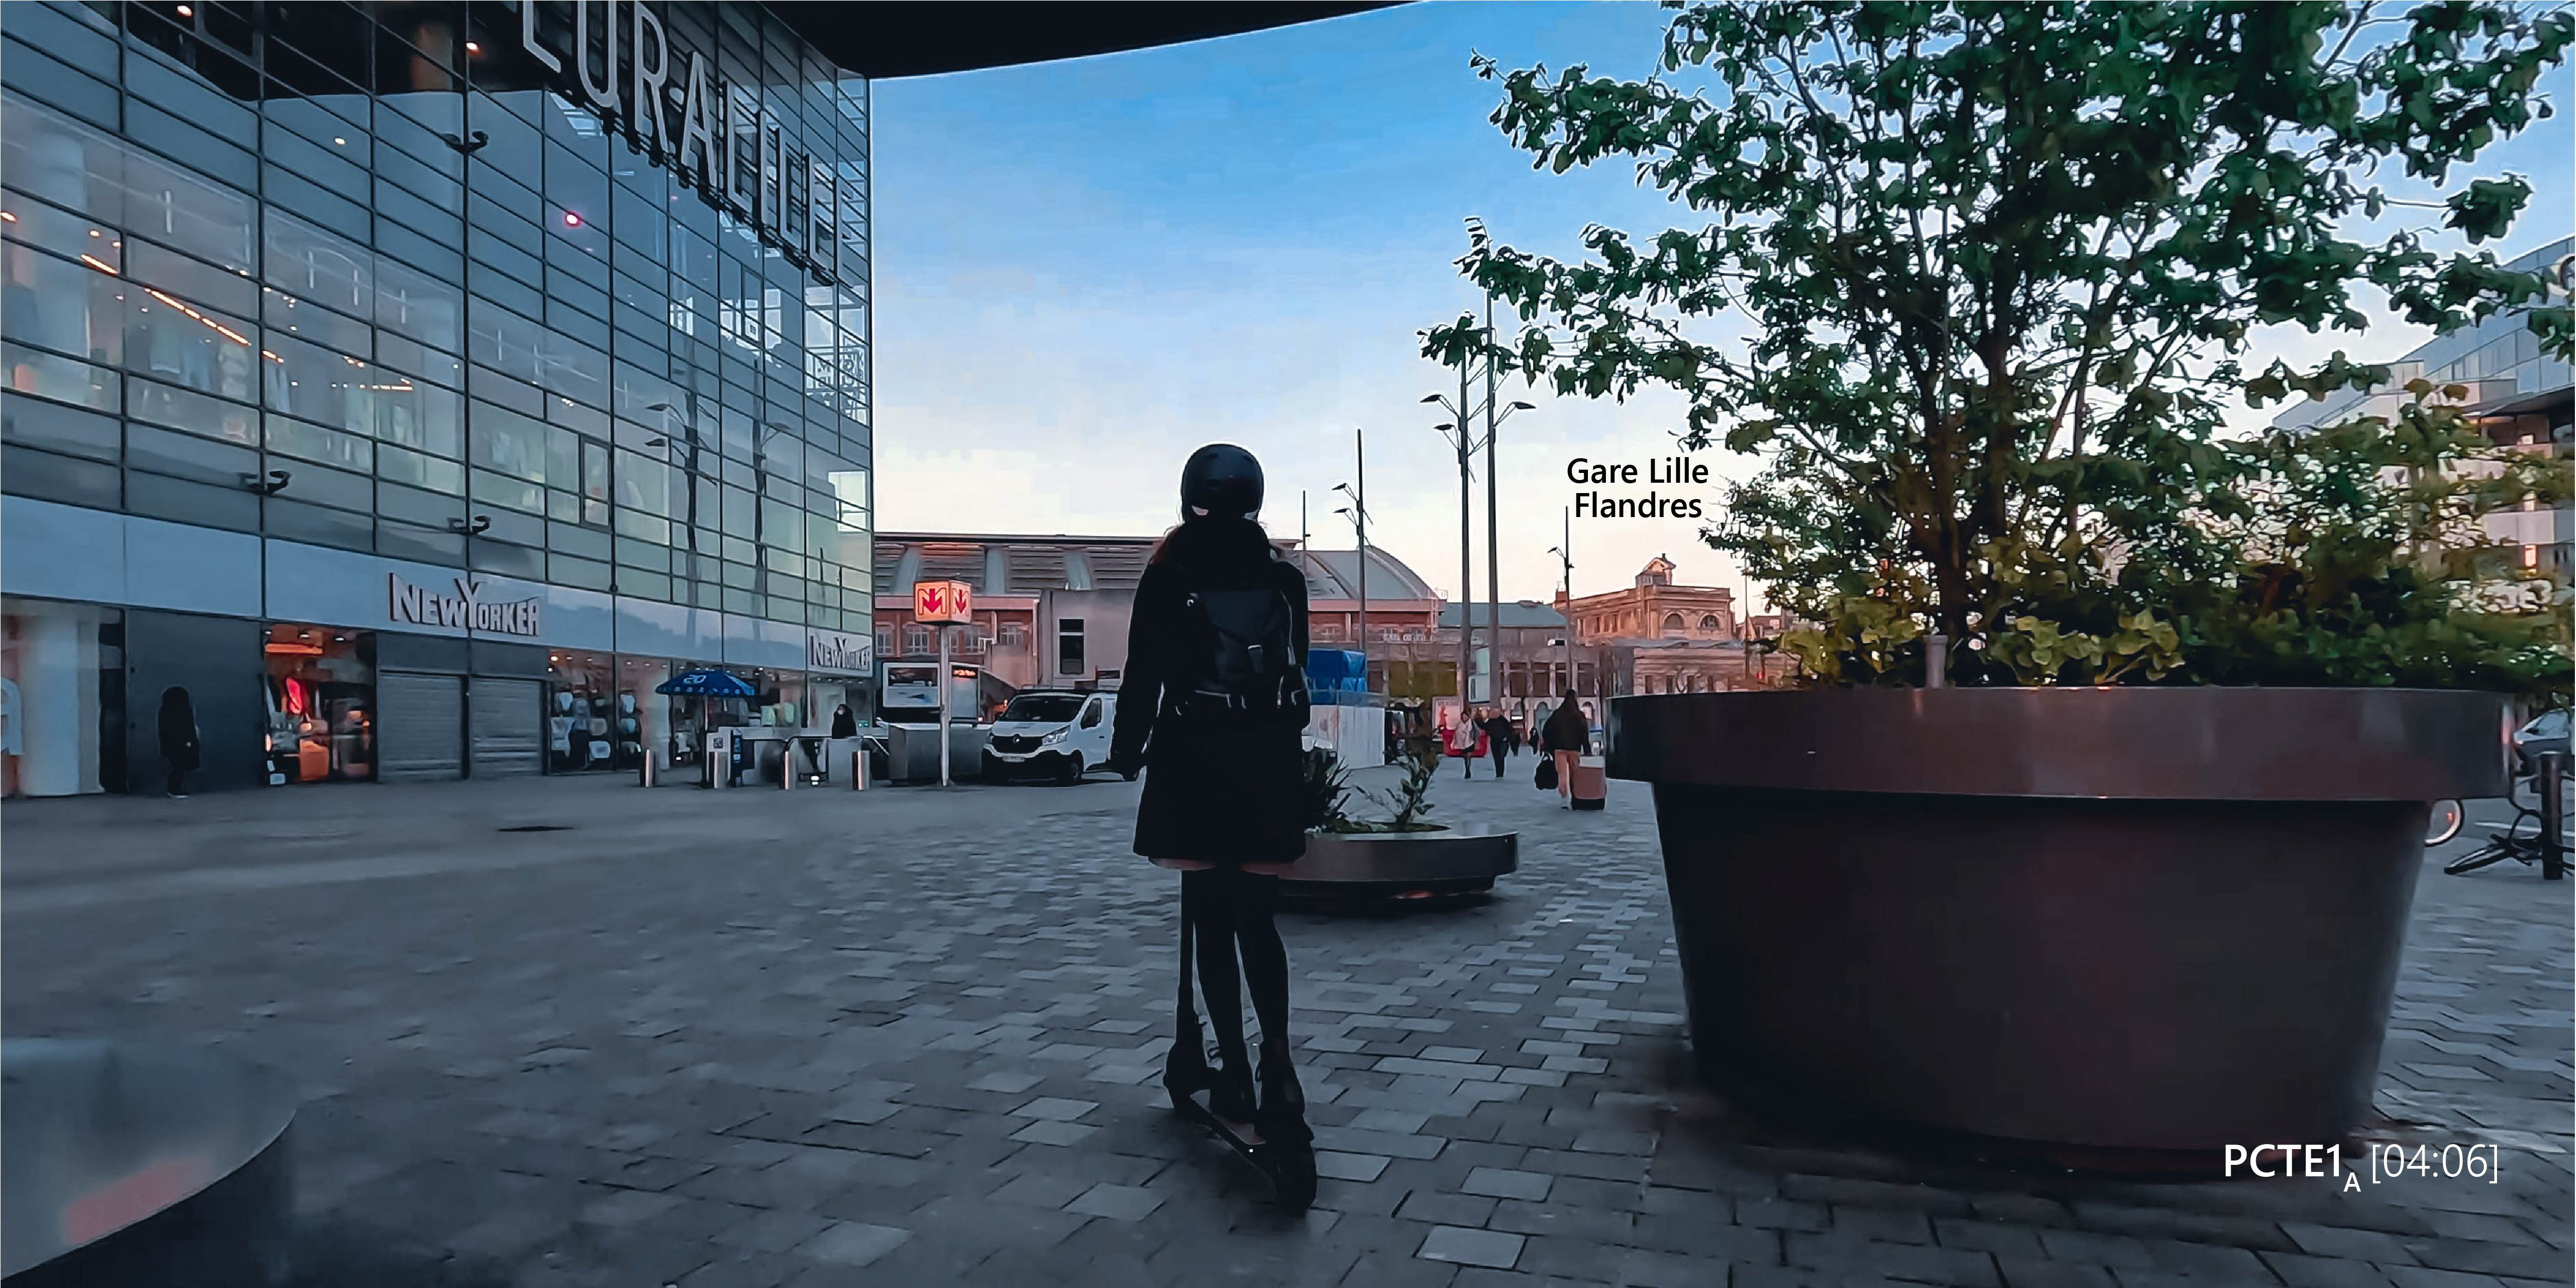
\includegraphics[width=0.75\columnwidth]{src/Figures/Annexes/Extrait_Video_PCTE1_Access_12.jpg}}
        \vspace{5pt}
        \begin{flushright}\scriptsize{
        Author: \textcolor{blue}{Dylan Moinse (2022)}
        }\end{flushright}
    \end{figure}

    % PCTE1 Photo Access 13
    \begin{figure}[h!]\vspace*{4pt}
        \caption*{Excerpt No. 13 from the video during the access segment (\(PCTE^{A}_{1}\))}
        \centerline{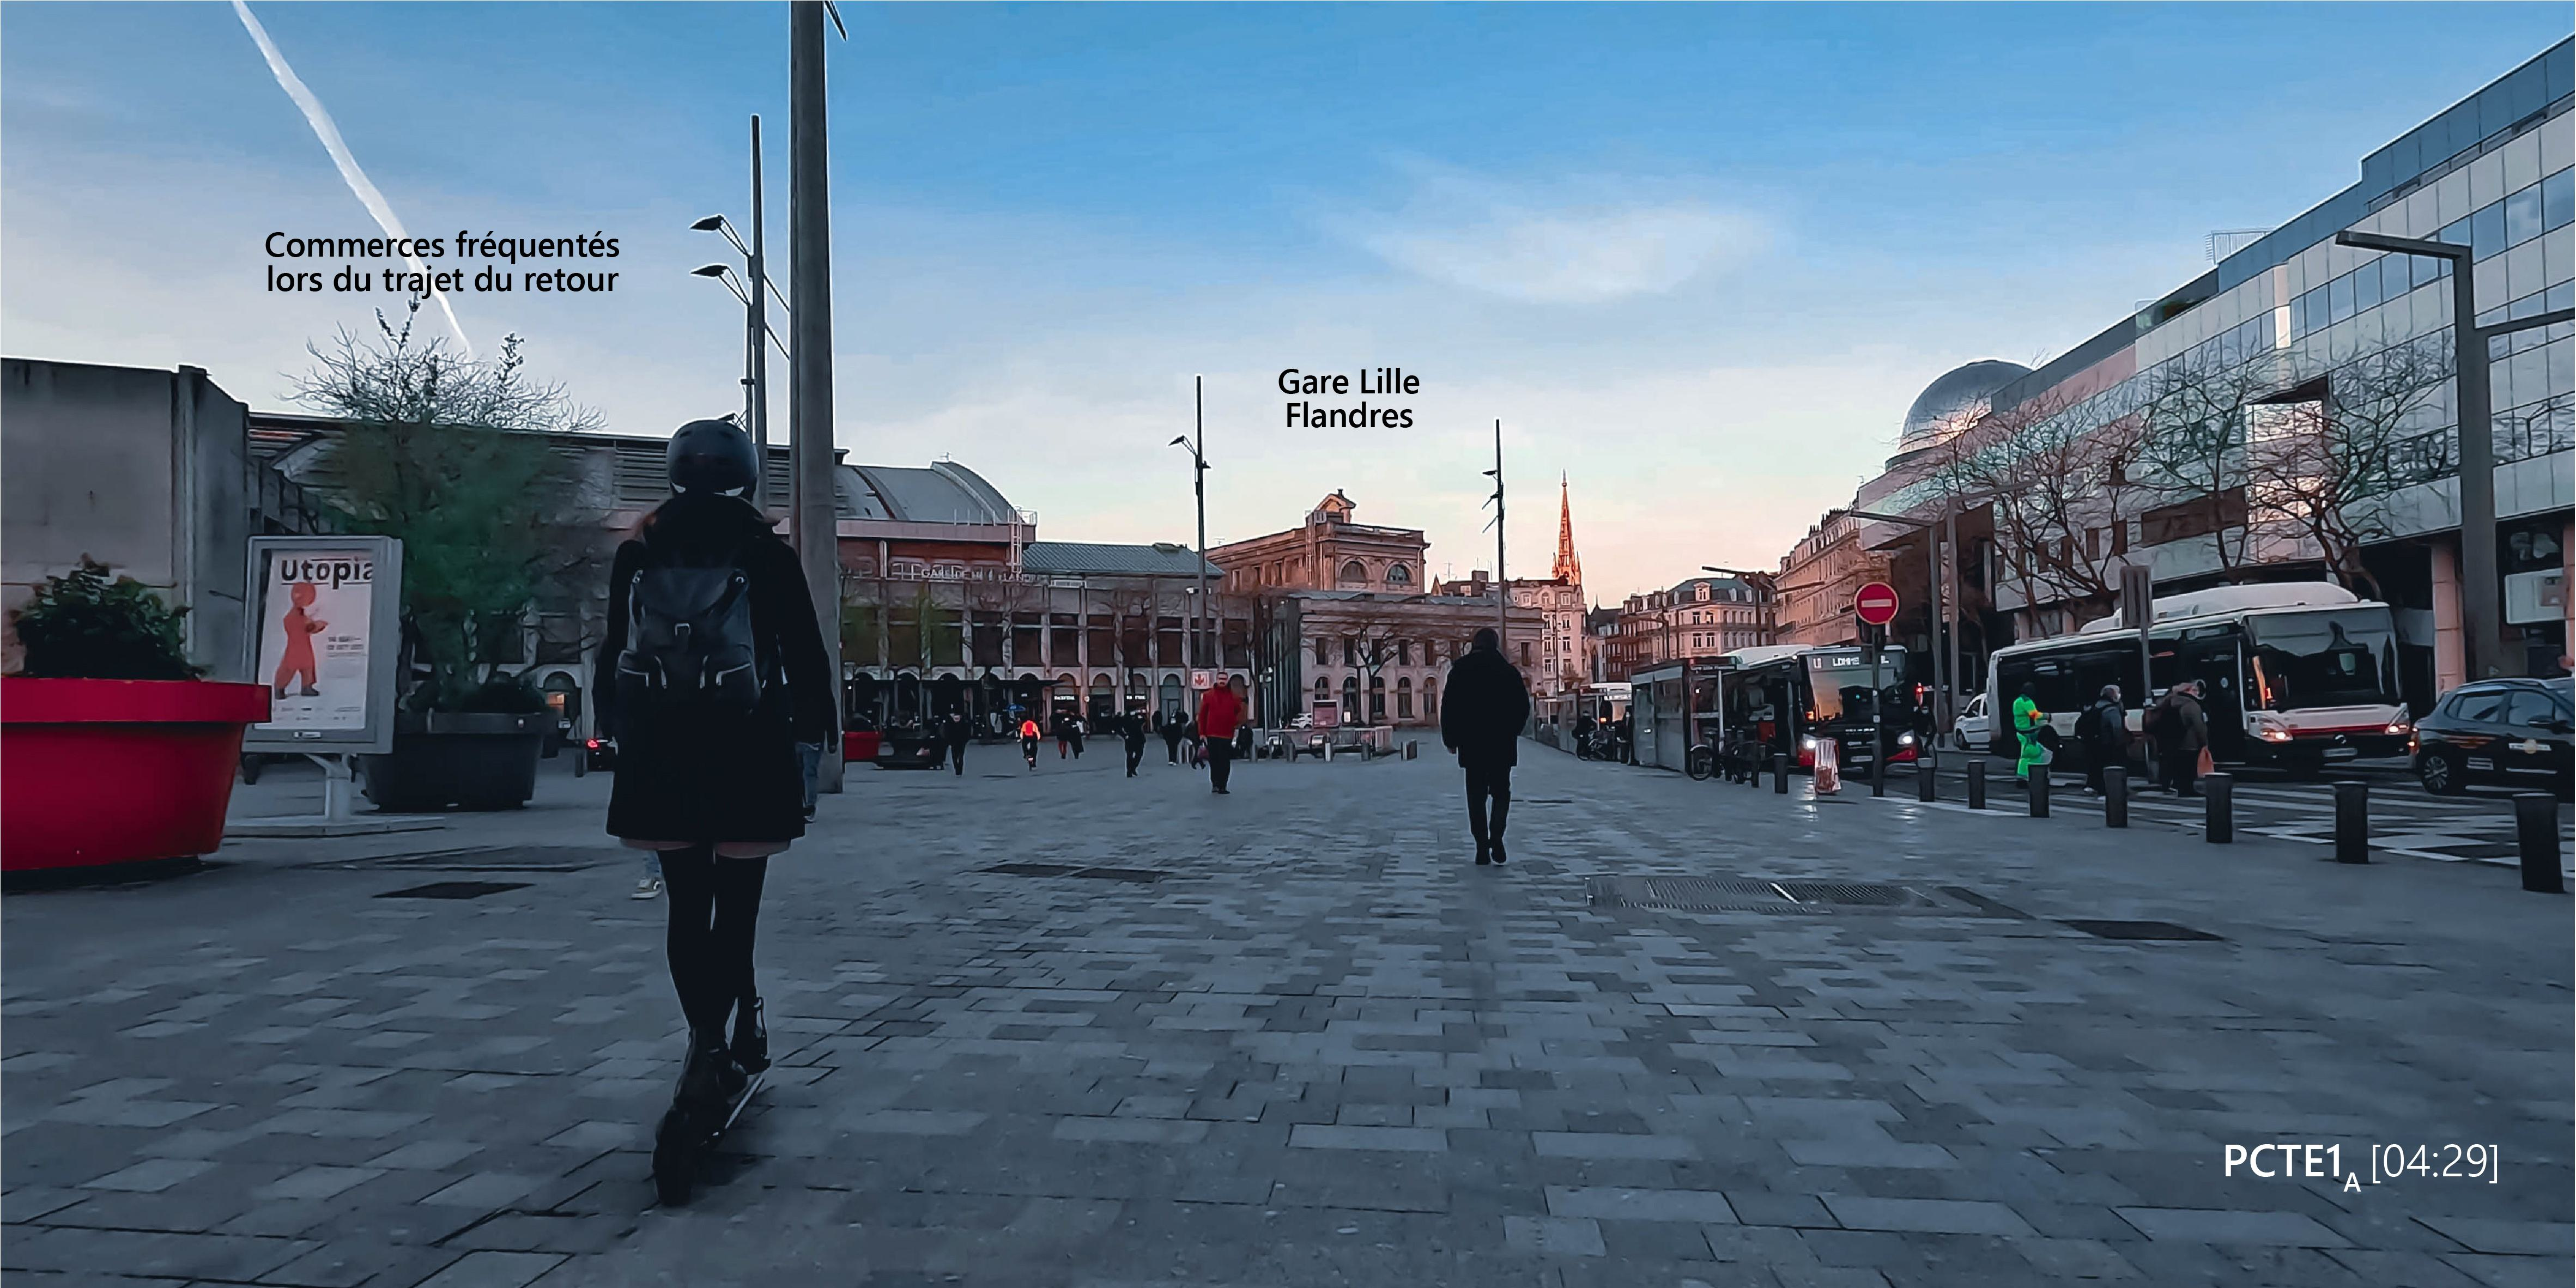
\includegraphics[width=0.75\columnwidth]{src/Figures/Annexes/Extrait_Video_PCTE1_Access_13.jpg}}
        \vspace{5pt}
        \begin{flushright}\scriptsize{
        Author: \textcolor{blue}{Dylan Moinse (2022)}
        }\end{flushright}
    \end{figure}


    % Photos PCTE1 TC
\subsubsection{Selection of Images Extracted During the Train Trip}

    % PCTE1 Photo TC 1
    \begin{figure}[h!]\vspace*{4pt}
        \caption*{Excerpt No. 1 from the video during the train trip (\(PCTE^{TC}_{1}\))}
        \centerline{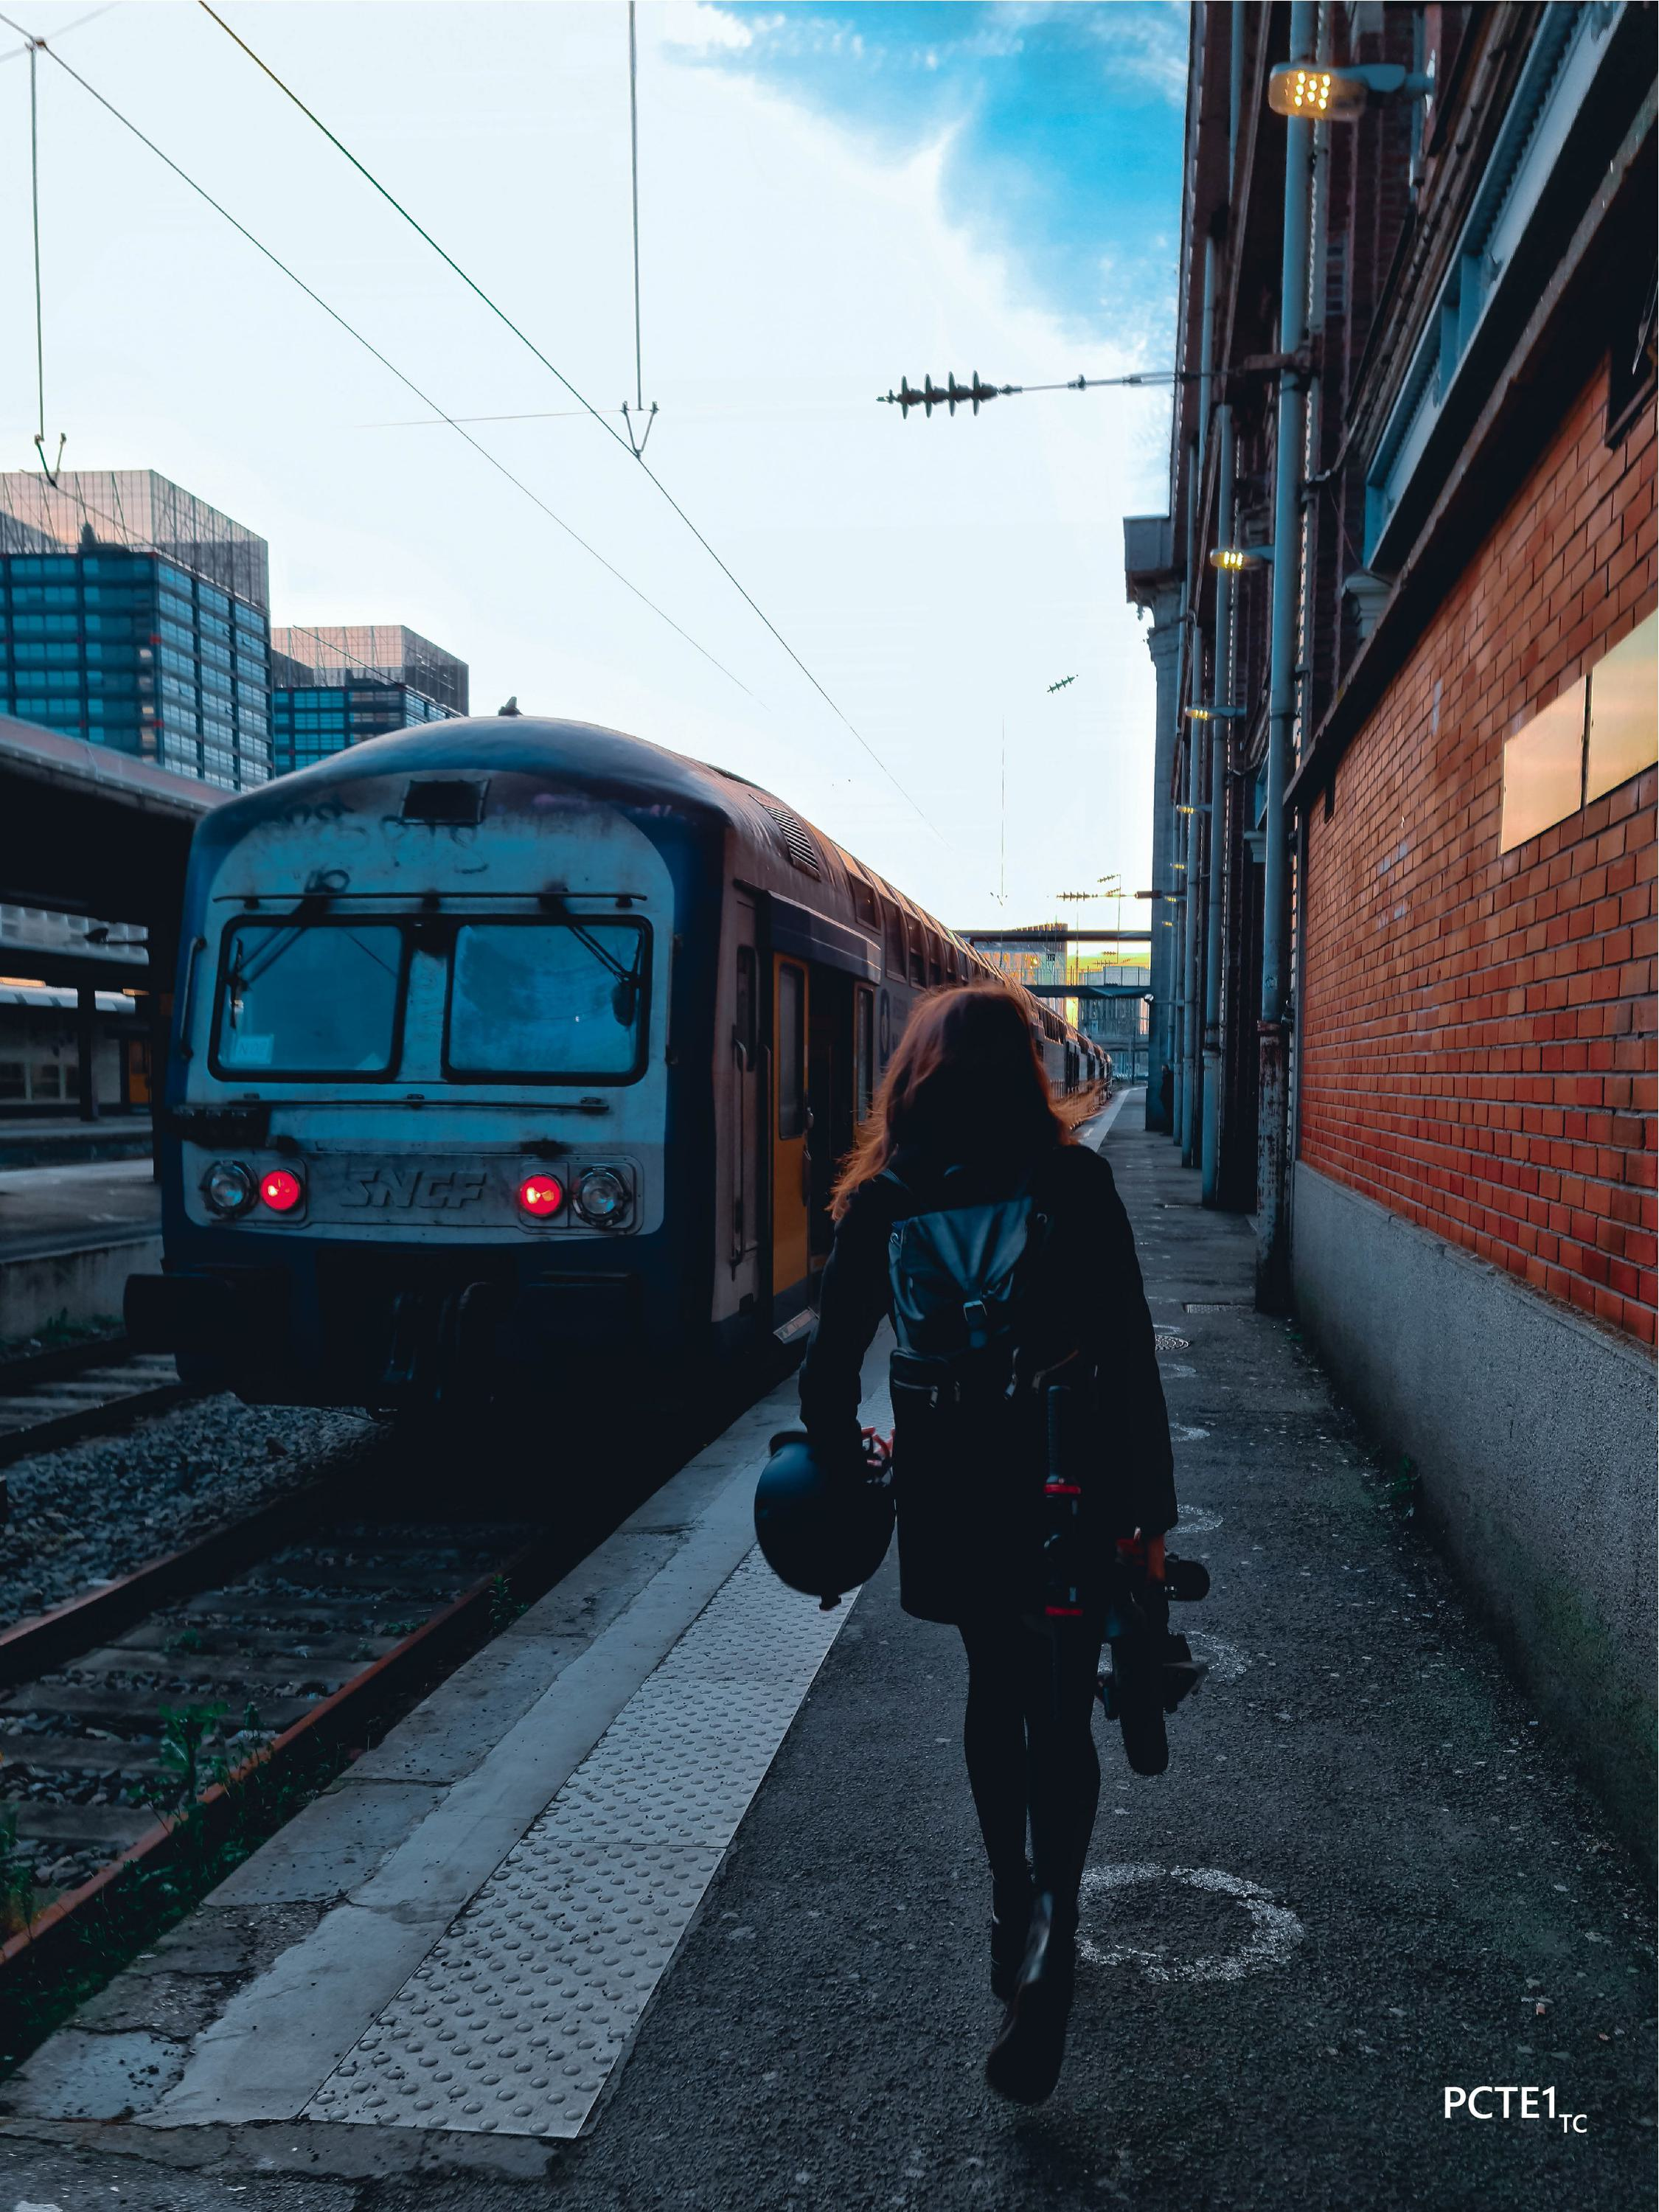
\includegraphics[width=0.5\columnwidth]{src/Figures/Annexes/Extrait_Video_PCTE1_TC_1.jpg}}
        \vspace{5pt}
        \begin{flushright}\scriptsize{
        Author: \textcolor{blue}{Dylan Moinse (2022)}
        }\end{flushright}
    \end{figure}

    % PCTE1 Photo TC 2
    \begin{figure}[h!]\vspace*{4pt}
        \caption*{Excerpt No. 2 from the video during the train trip (\(PCTE^{TC}_{1}\))}
        \centerline{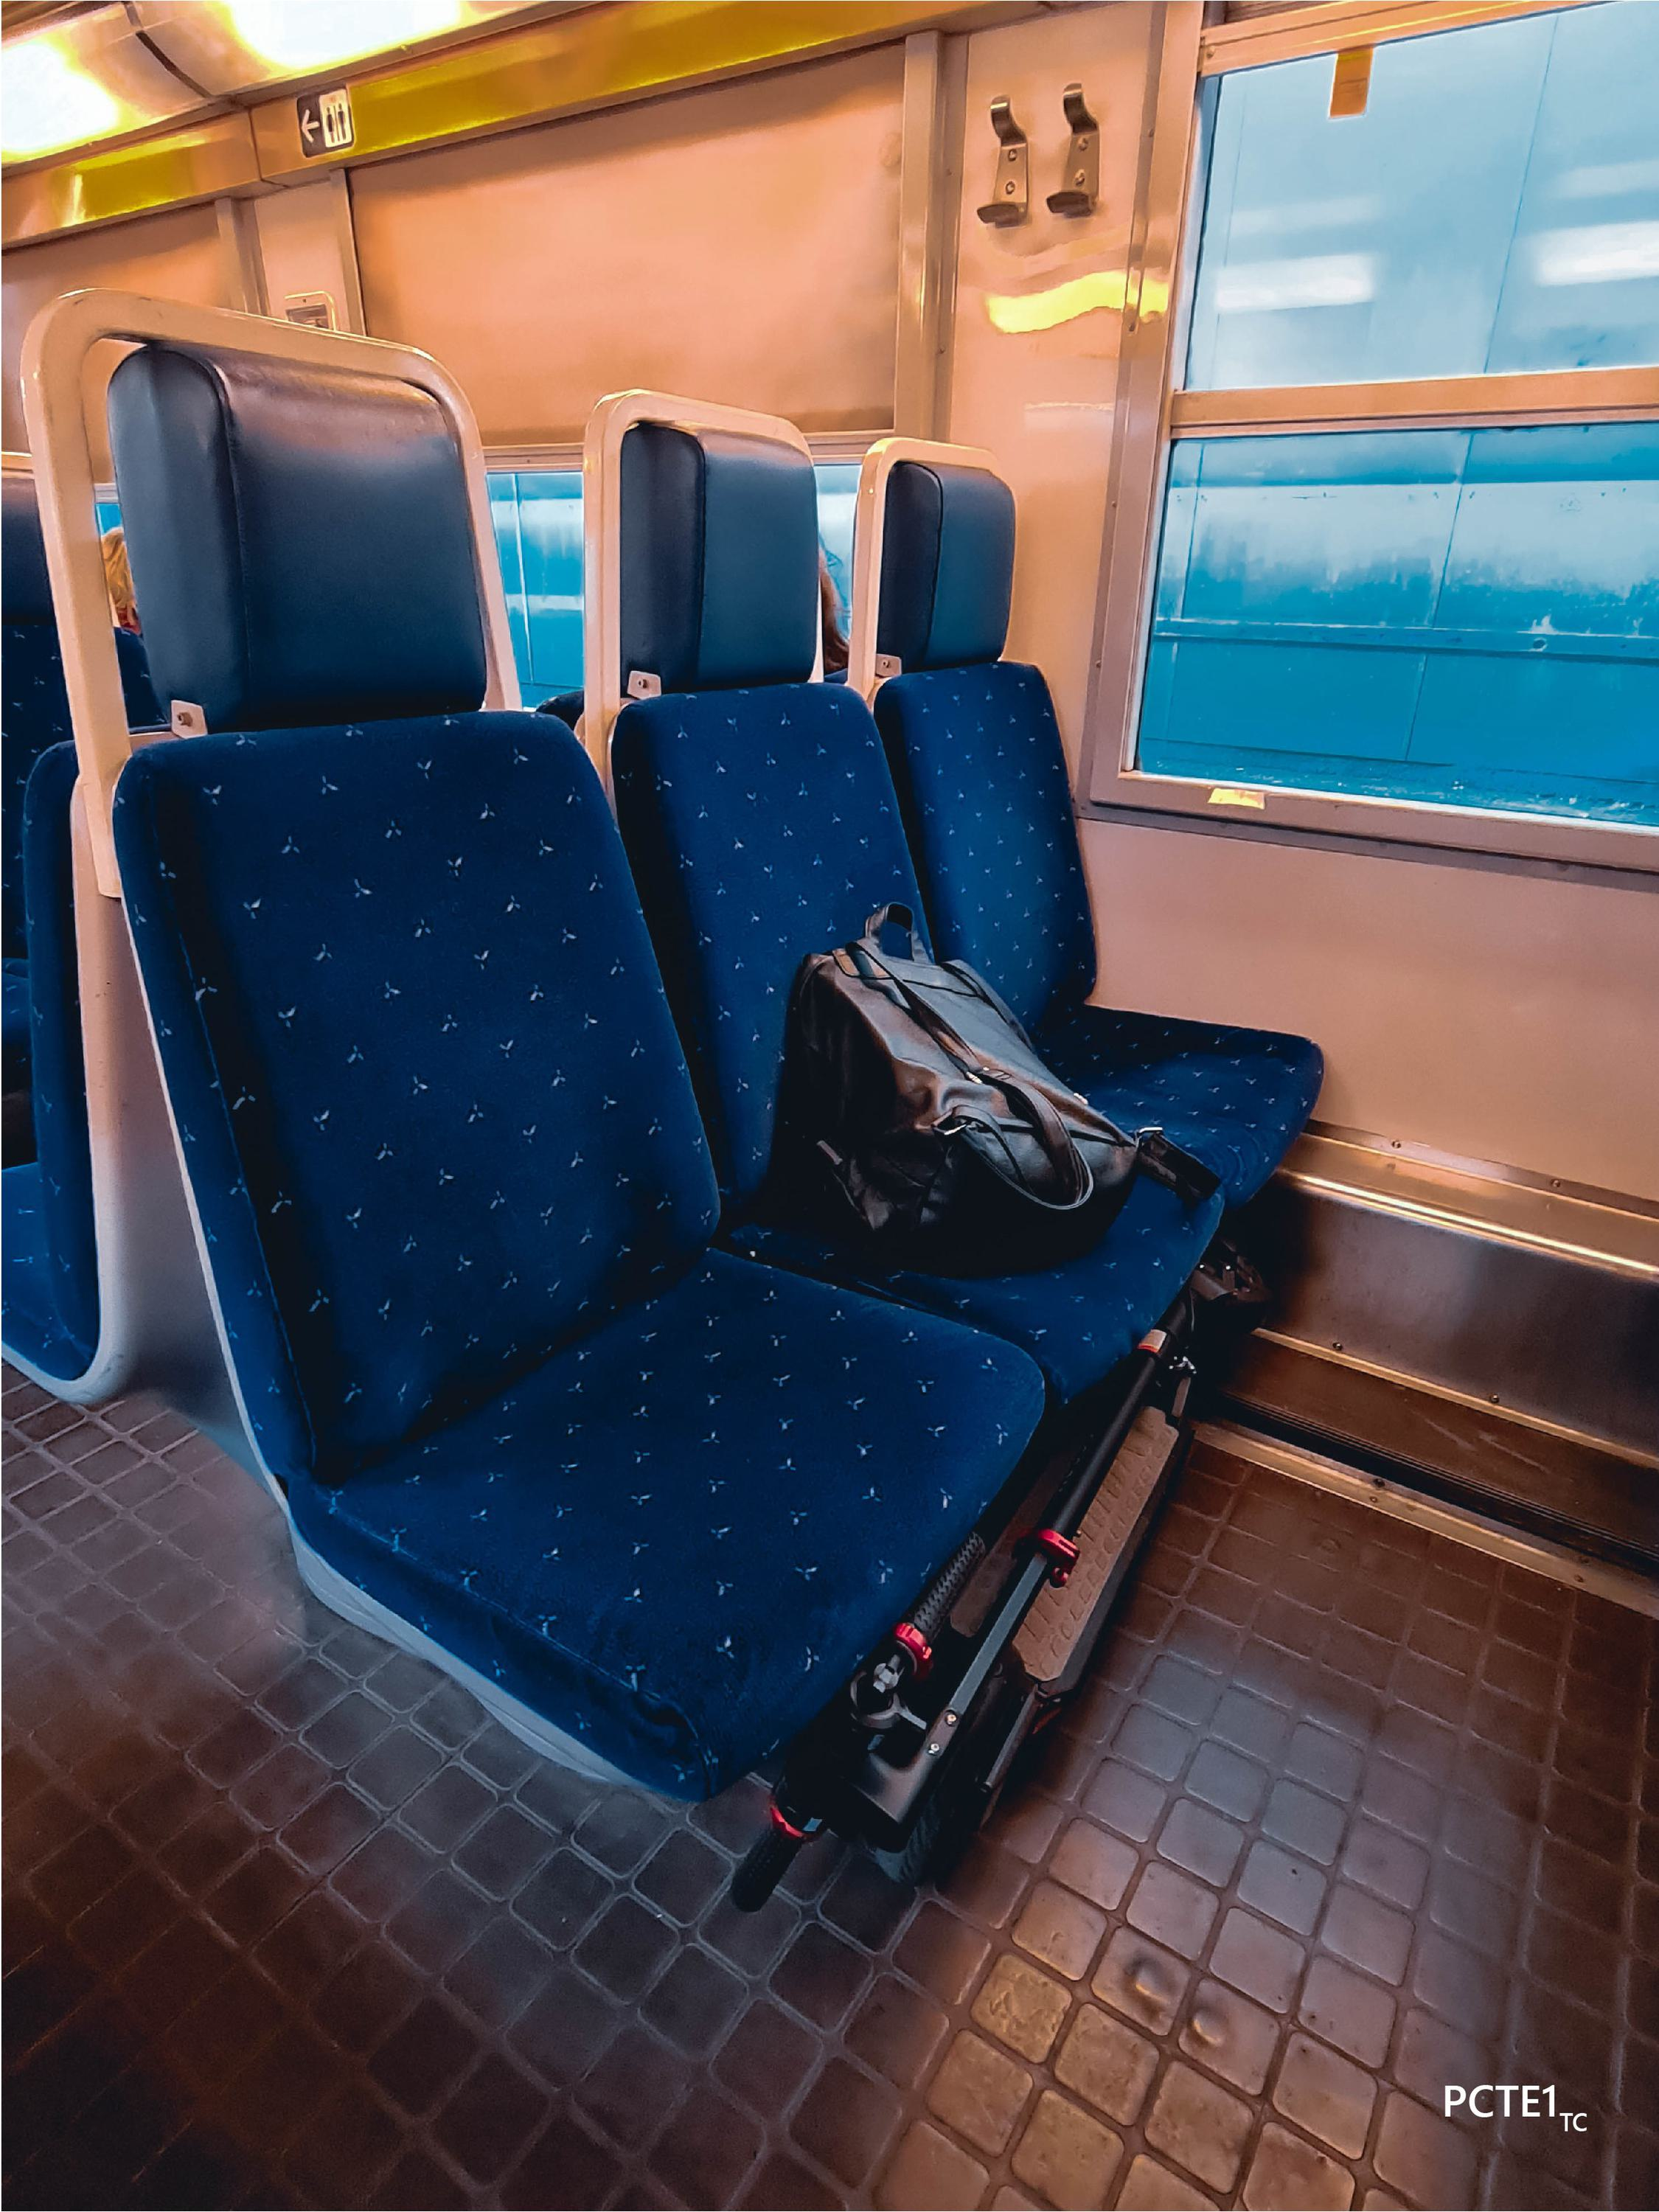
\includegraphics[width=0.5\columnwidth]{src/Figures/Annexes/Extrait_Video_PCTE1_TC_2.jpg}}
        \vspace{5pt}
        \begin{flushright}\scriptsize{
        Author: \textcolor{blue}{Dylan Moinse (2022)}
        }\end{flushright}
    \end{figure}

    % PCTE1 Photo TC 3
    \begin{figure}[h!]\vspace*{4pt}
        \caption*{Excerpt No. 3 from the video during the train trip (\(PCTE^{TC}_{1}\))}
        \centerline{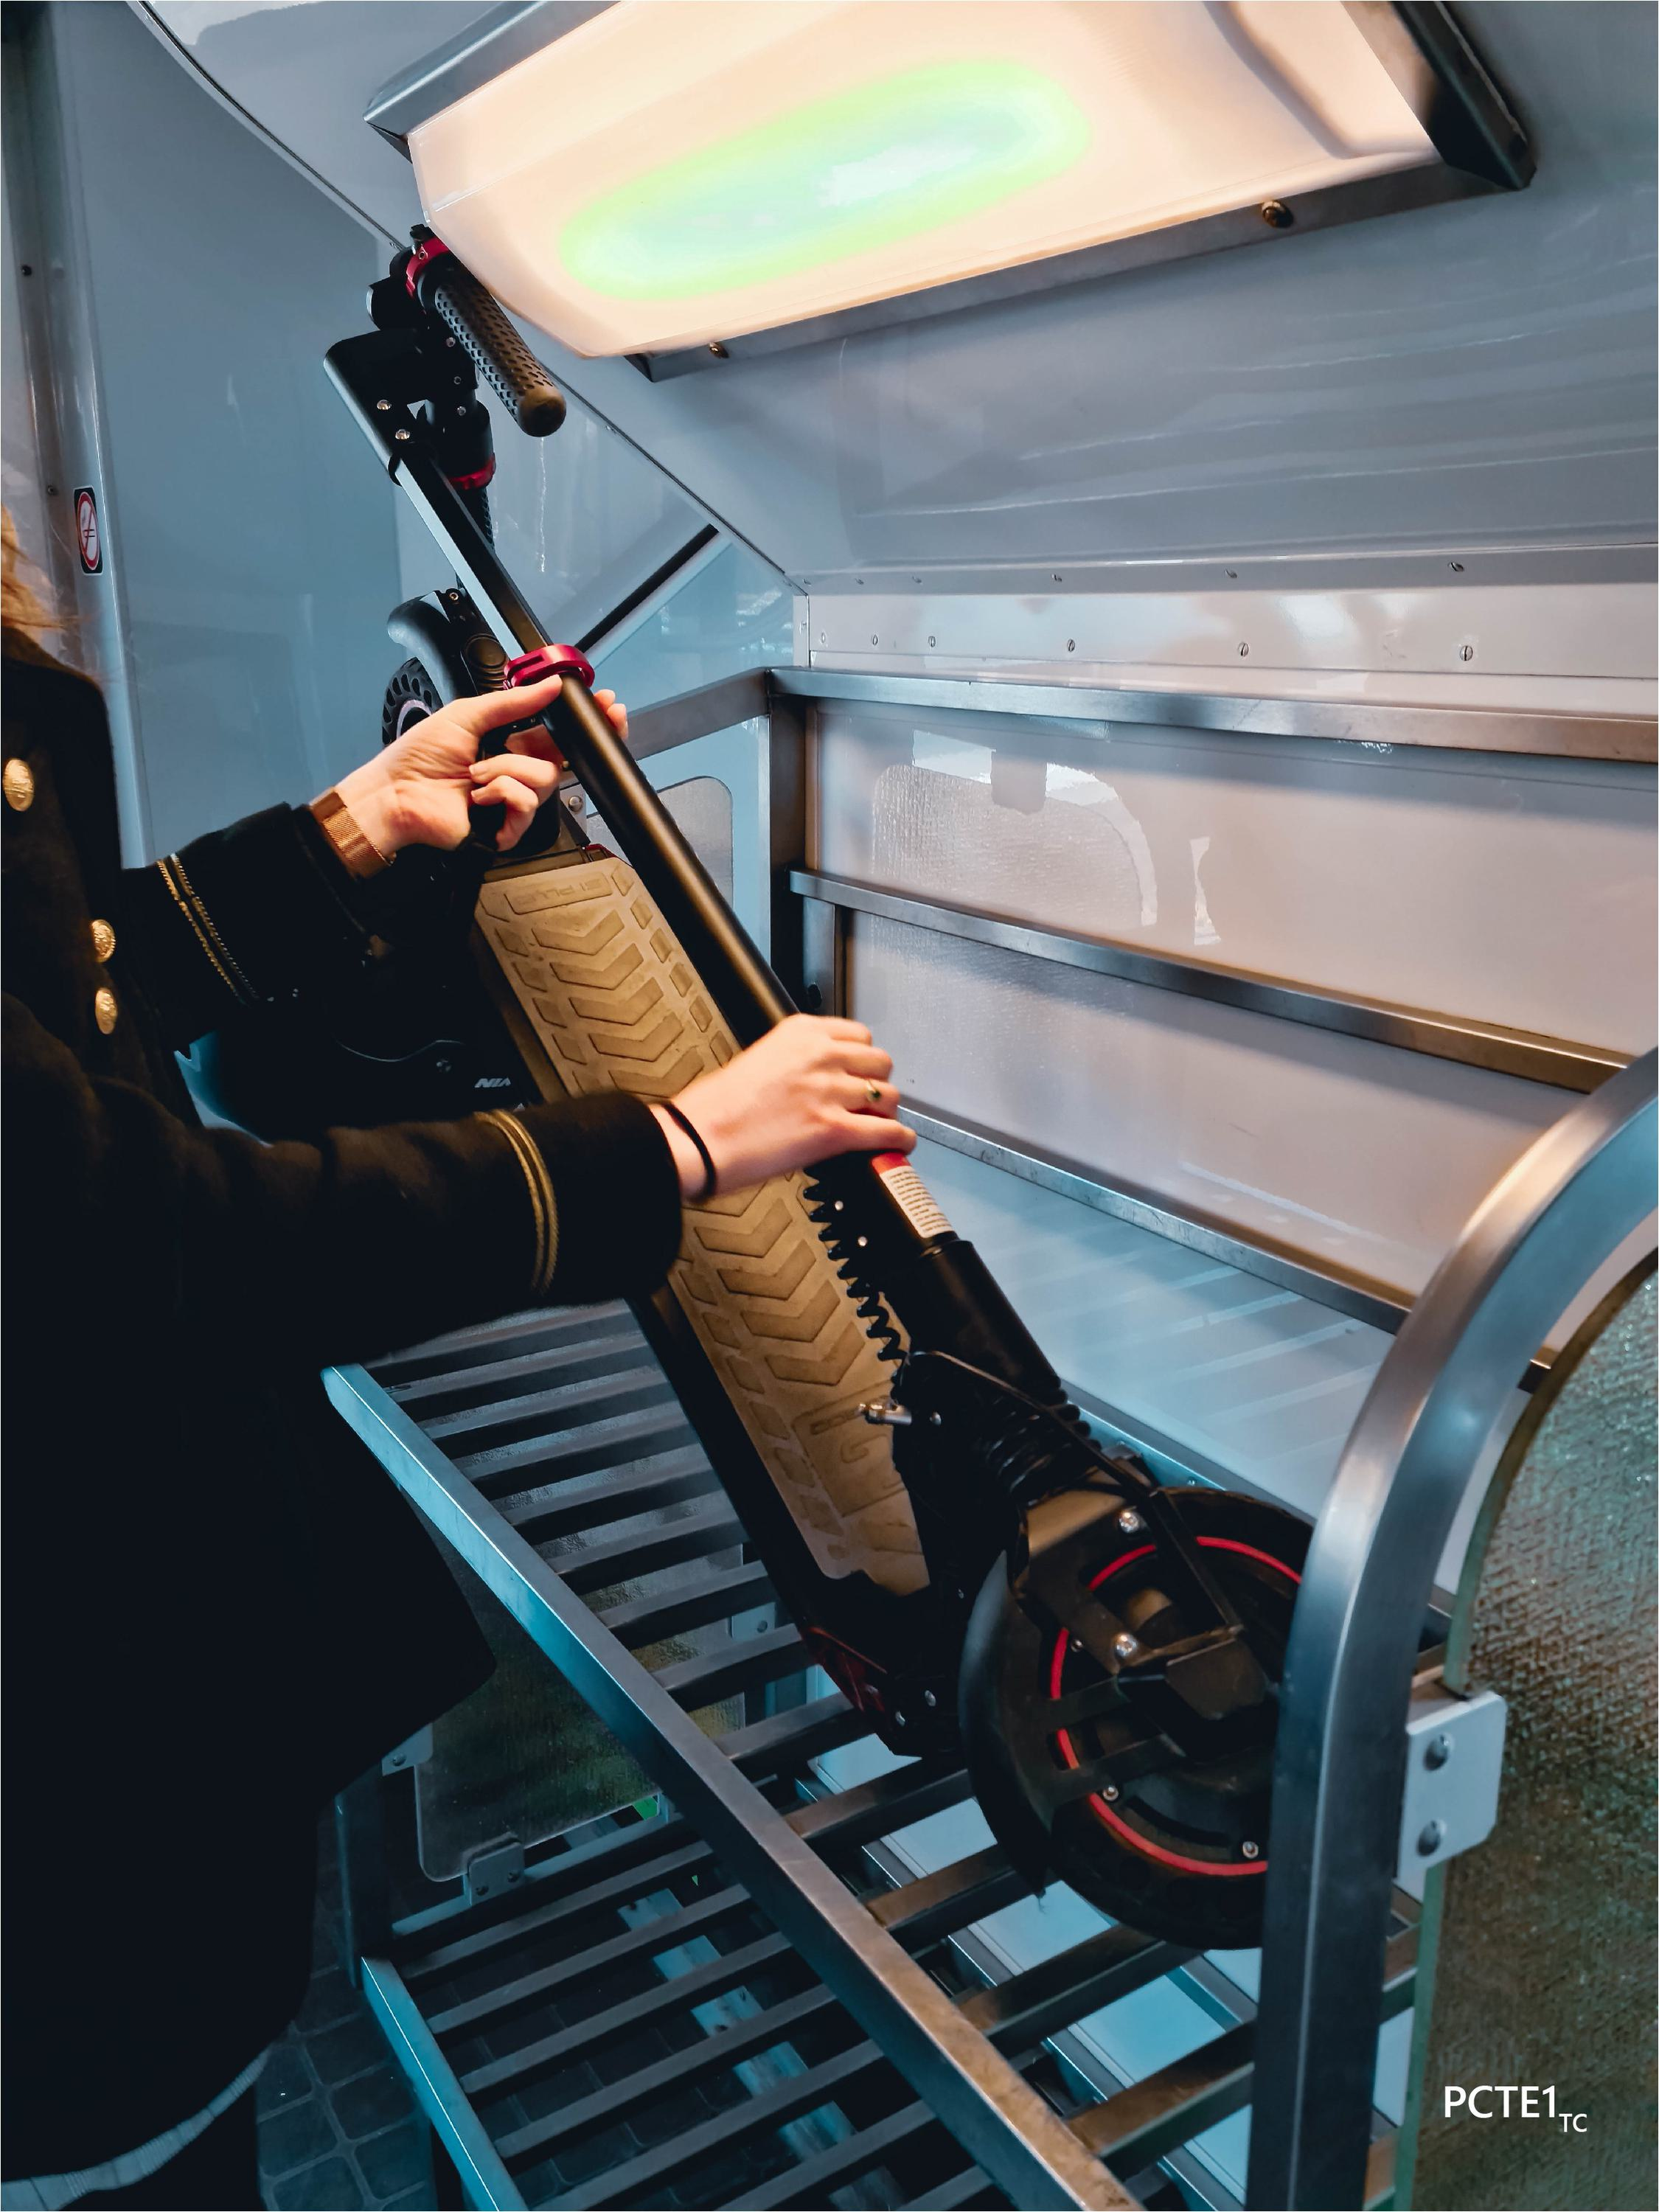
\includegraphics[width=0.5\columnwidth]{src/Figures/Annexes/Extrait_Video_PCTE1_TC_3.jpg}}
        \vspace{5pt}
        \begin{flushright}\scriptsize{
        Author: \textcolor{blue}{Dylan Moinse (2022)}
        }\end{flushright}
    \end{figure}

    % Photos PCTE1 egress
\subsubsection{Selection of Images Extracted During the Egress Trip}

    % PCTE1 Photo Egress 1
    \begin{figure}[h!]\vspace*{4pt}
        \caption*{Excerpt No. 1 from the video during the egress segment (\(PCTE^{E}_{1}\))}
        \centerline{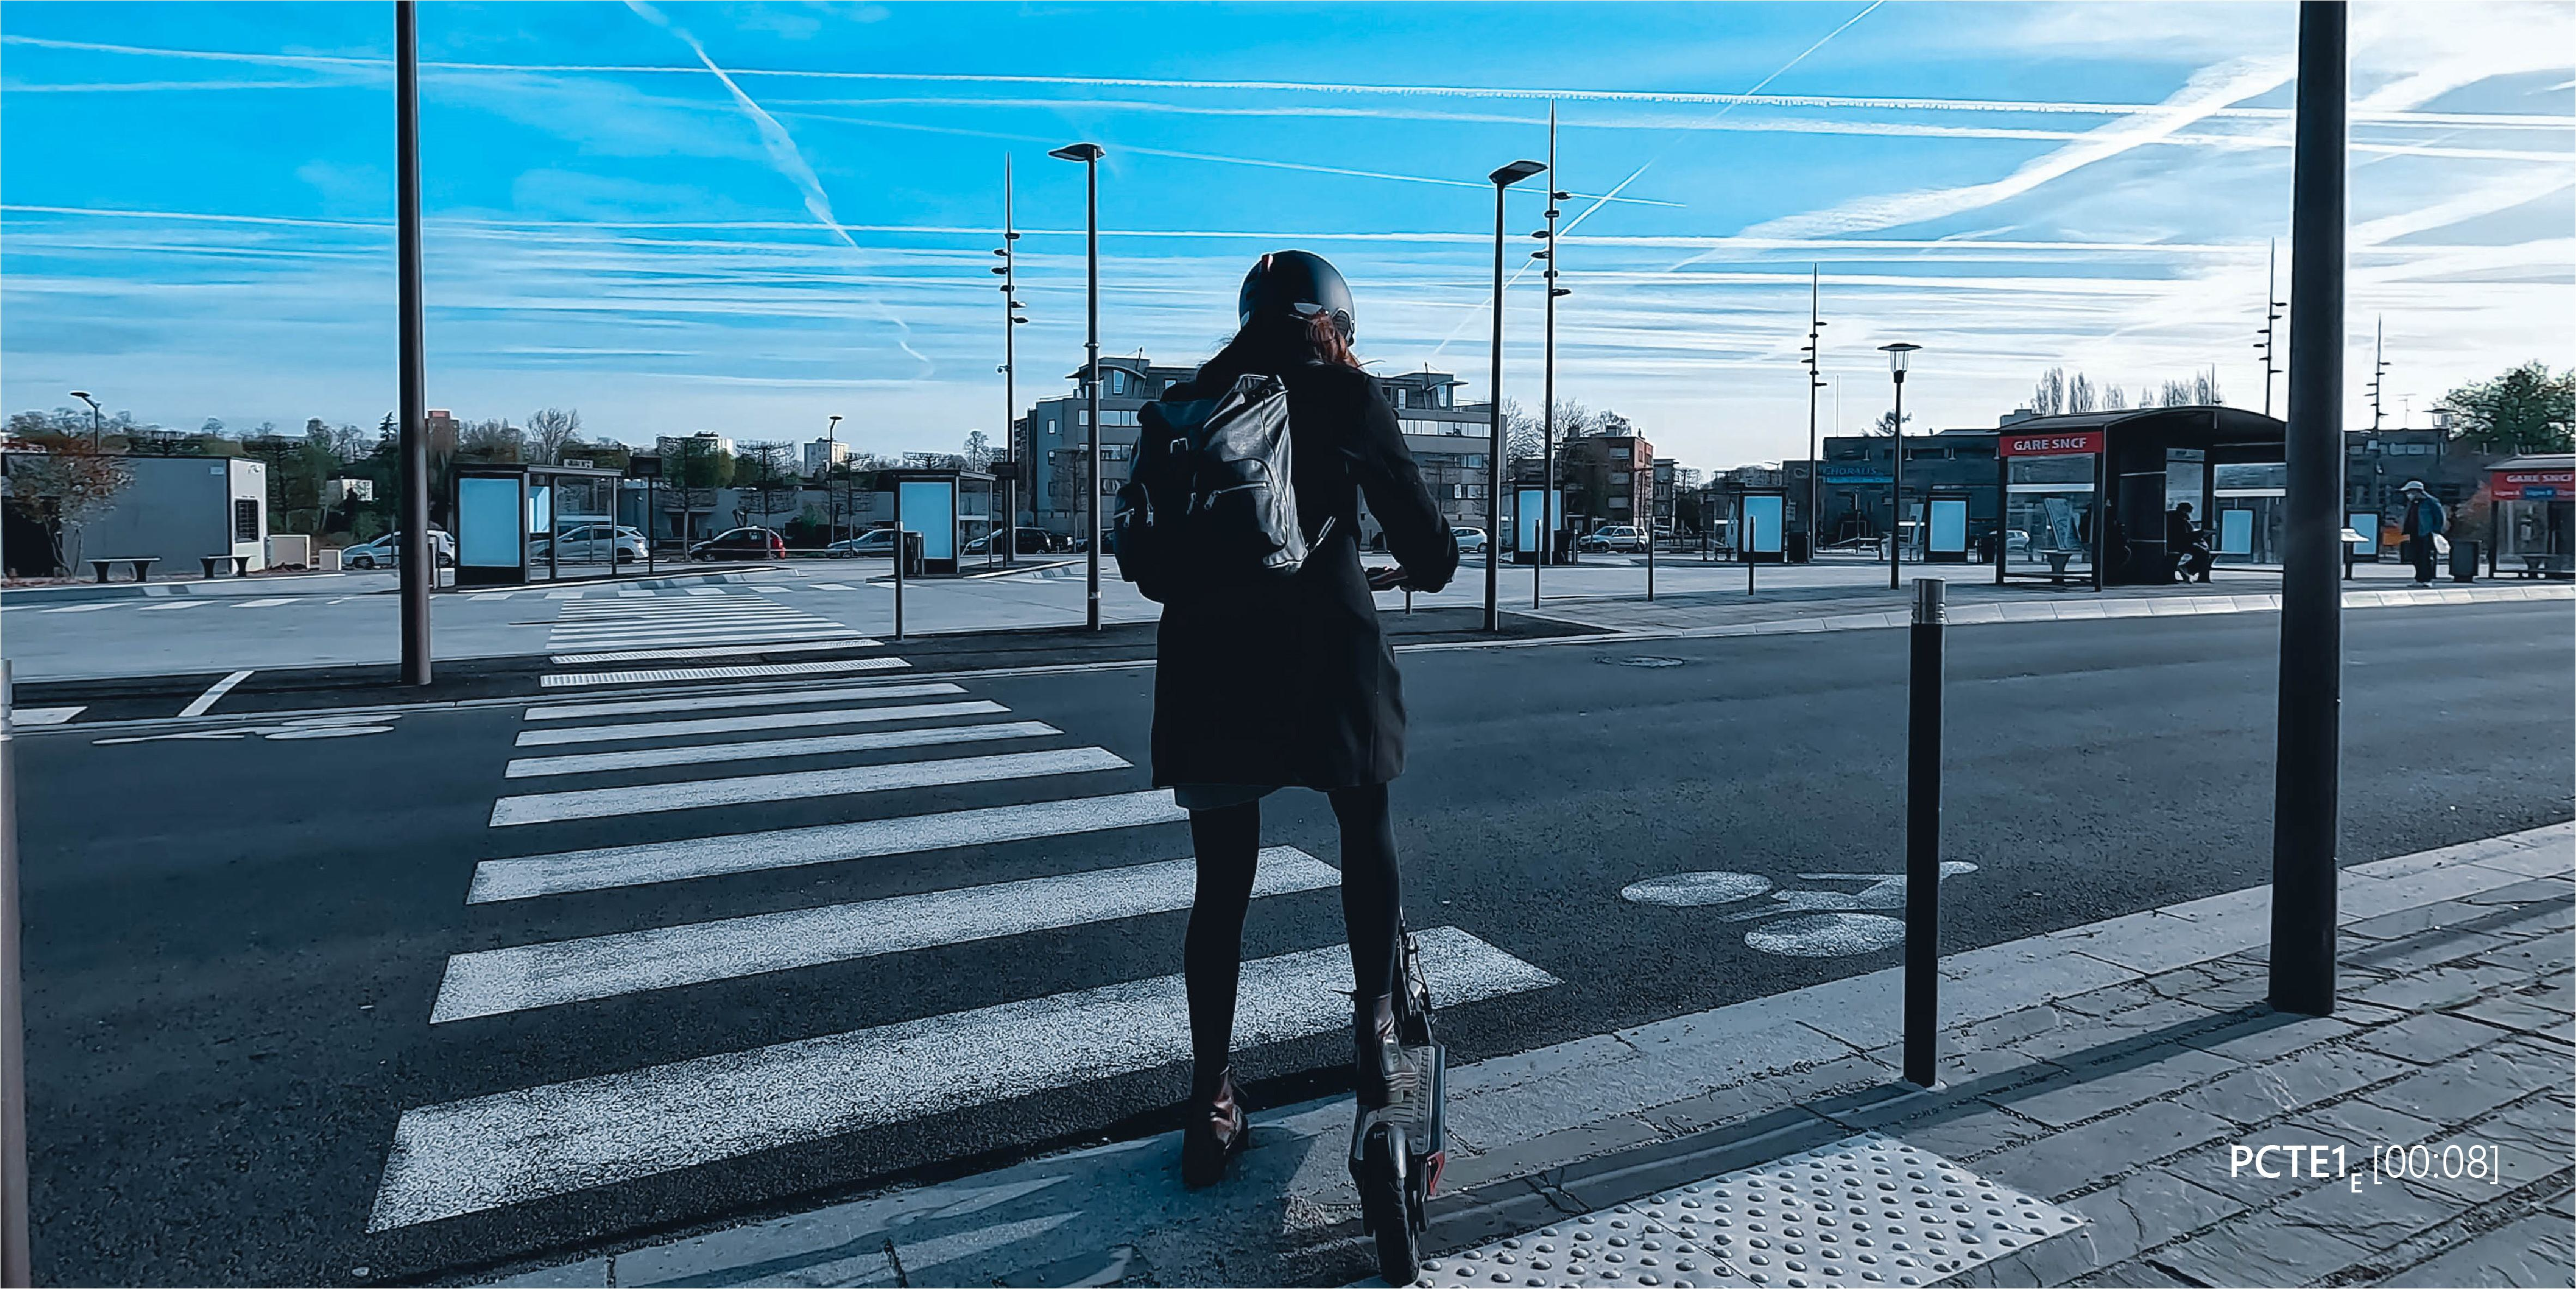
\includegraphics[width=0.75\columnwidth]{src/Figures/Annexes/Extrait_Video_PCTE1_Egress_1.jpg}}
        \vspace{5pt}
        \begin{flushright}\scriptsize{
        Author: \textcolor{blue}{Dylan Moinse (2022)}
        }\end{flushright}
    \end{figure}

    % PCTE1 Photo Egress 2
    \begin{figure}[h!]\vspace*{4pt}
        \caption*{Excerpt No. 2 from the video during the egress segment (\(PCTE^{E}_{1}\))}
        \centerline{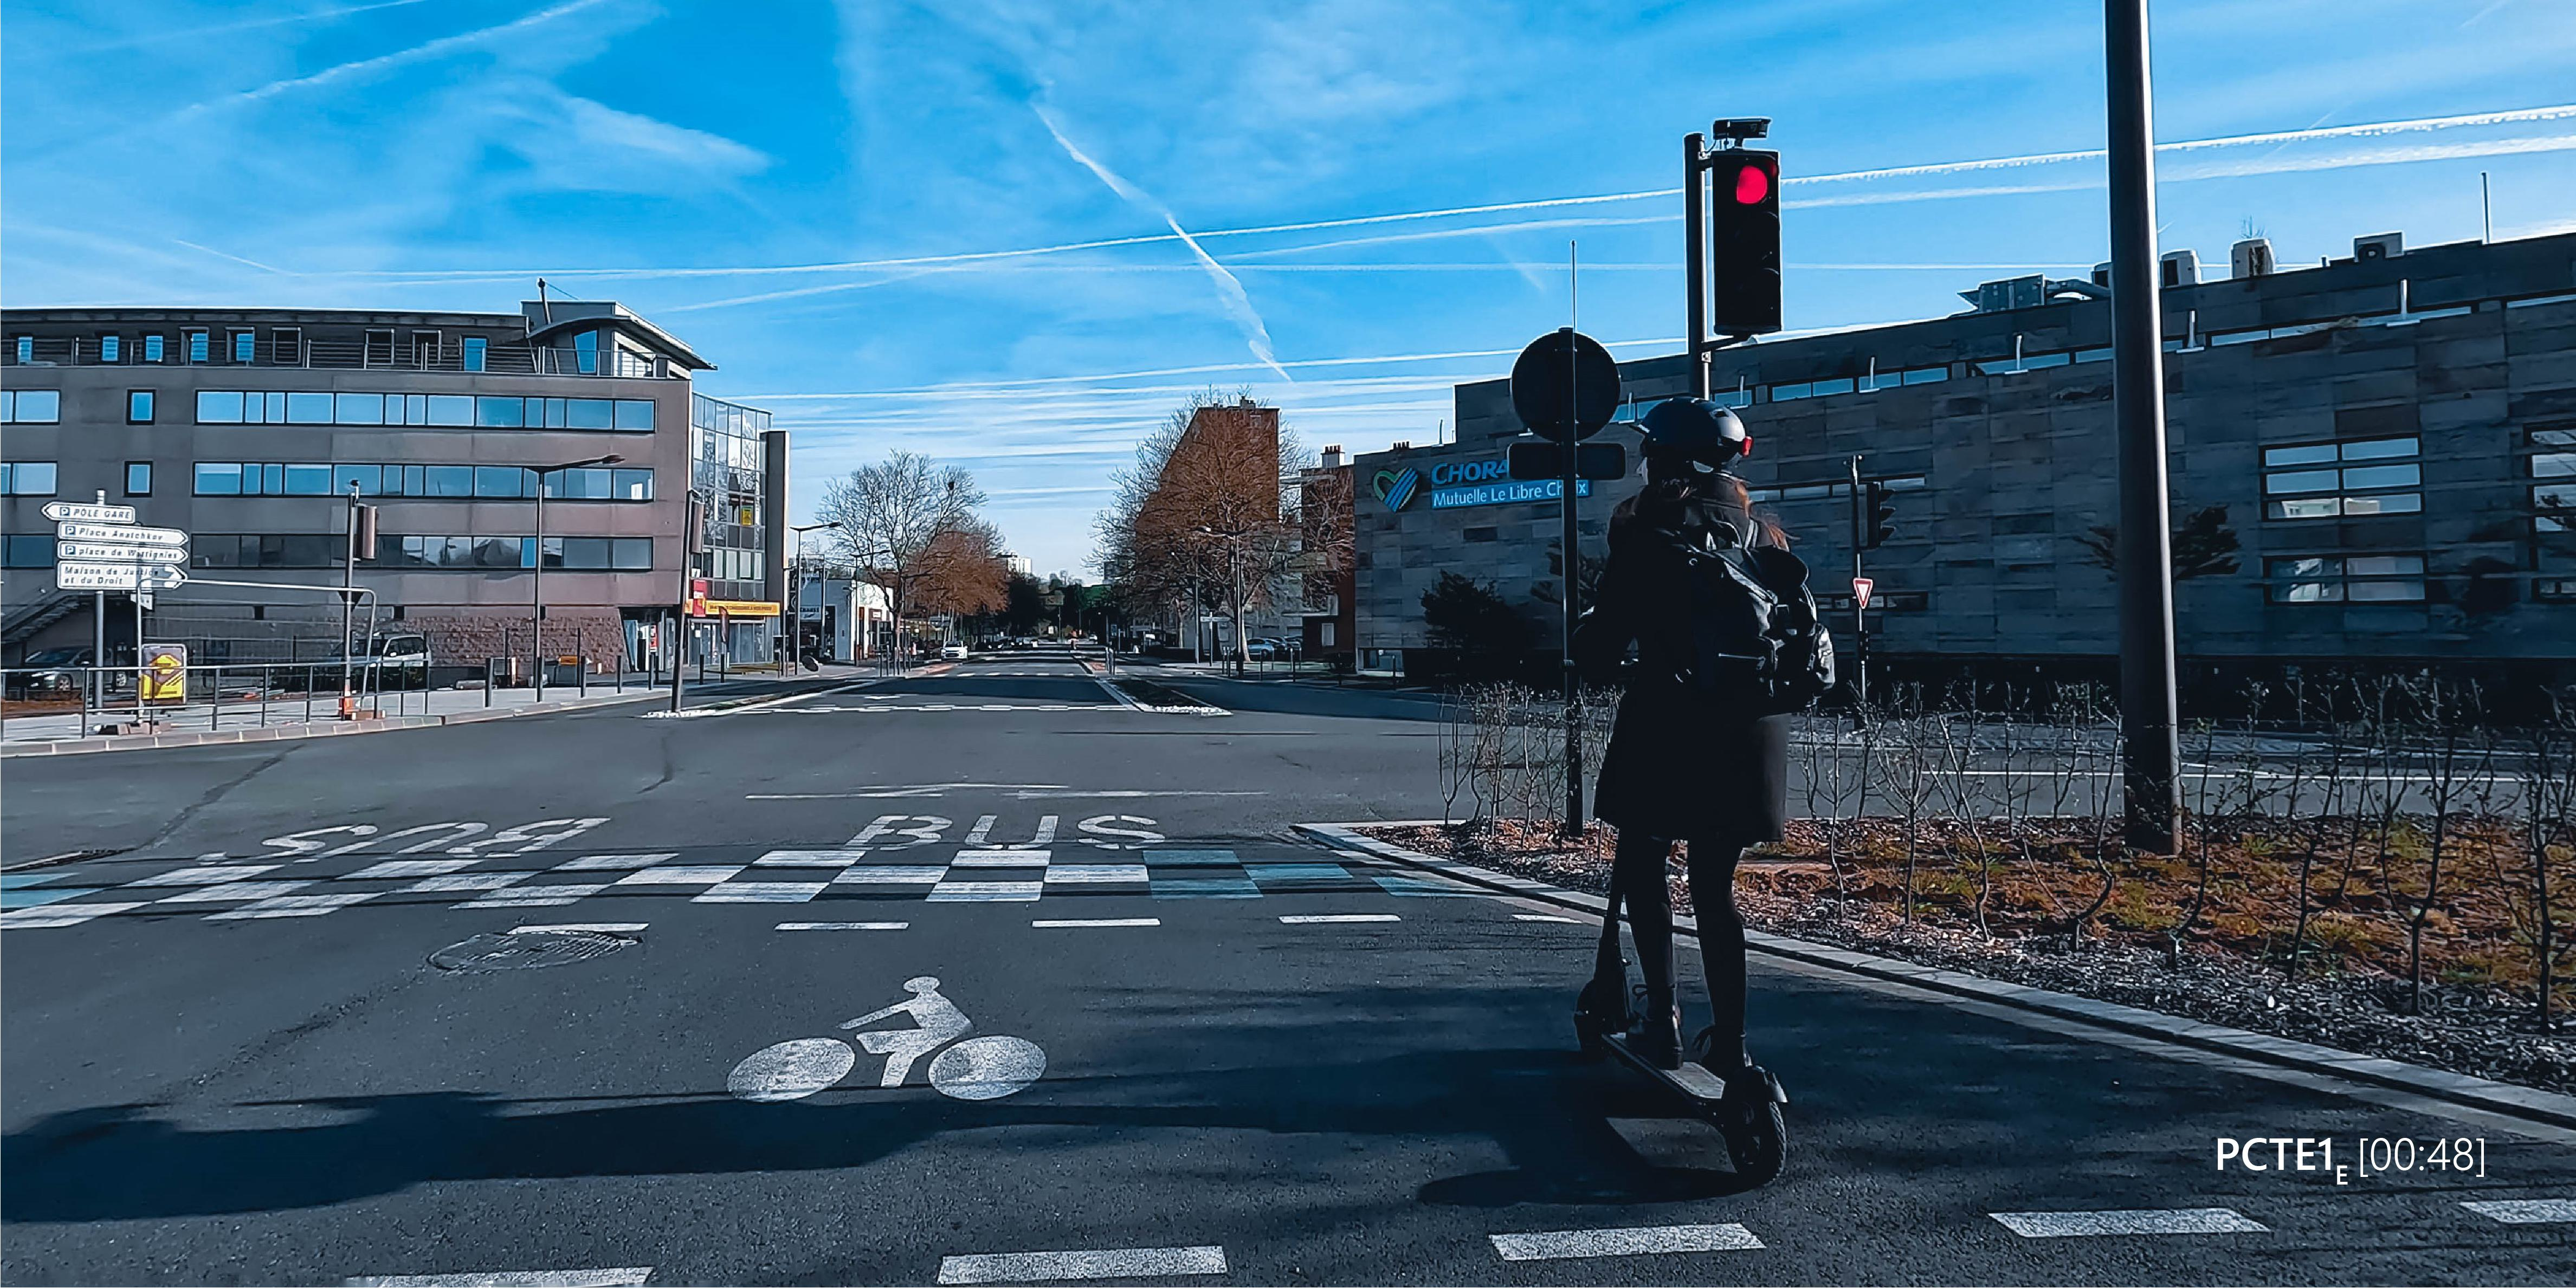
\includegraphics[width=0.75\columnwidth]{src/Figures/Annexes/Extrait_Video_PCTE1_Egress_2.jpg}}
        \vspace{5pt}
        \begin{flushright}\scriptsize{
        Author: \textcolor{blue}{Dylan Moinse (2022)}
        }\end{flushright}
    \end{figure}

    % PCTE1 Photo Egress 3
    \begin{figure}[h!]\vspace*{4pt}
        \caption*{Excerpt No. 3 from the video during the egress segment (\(PCTE^{E}_{1}\))}
        \centerline{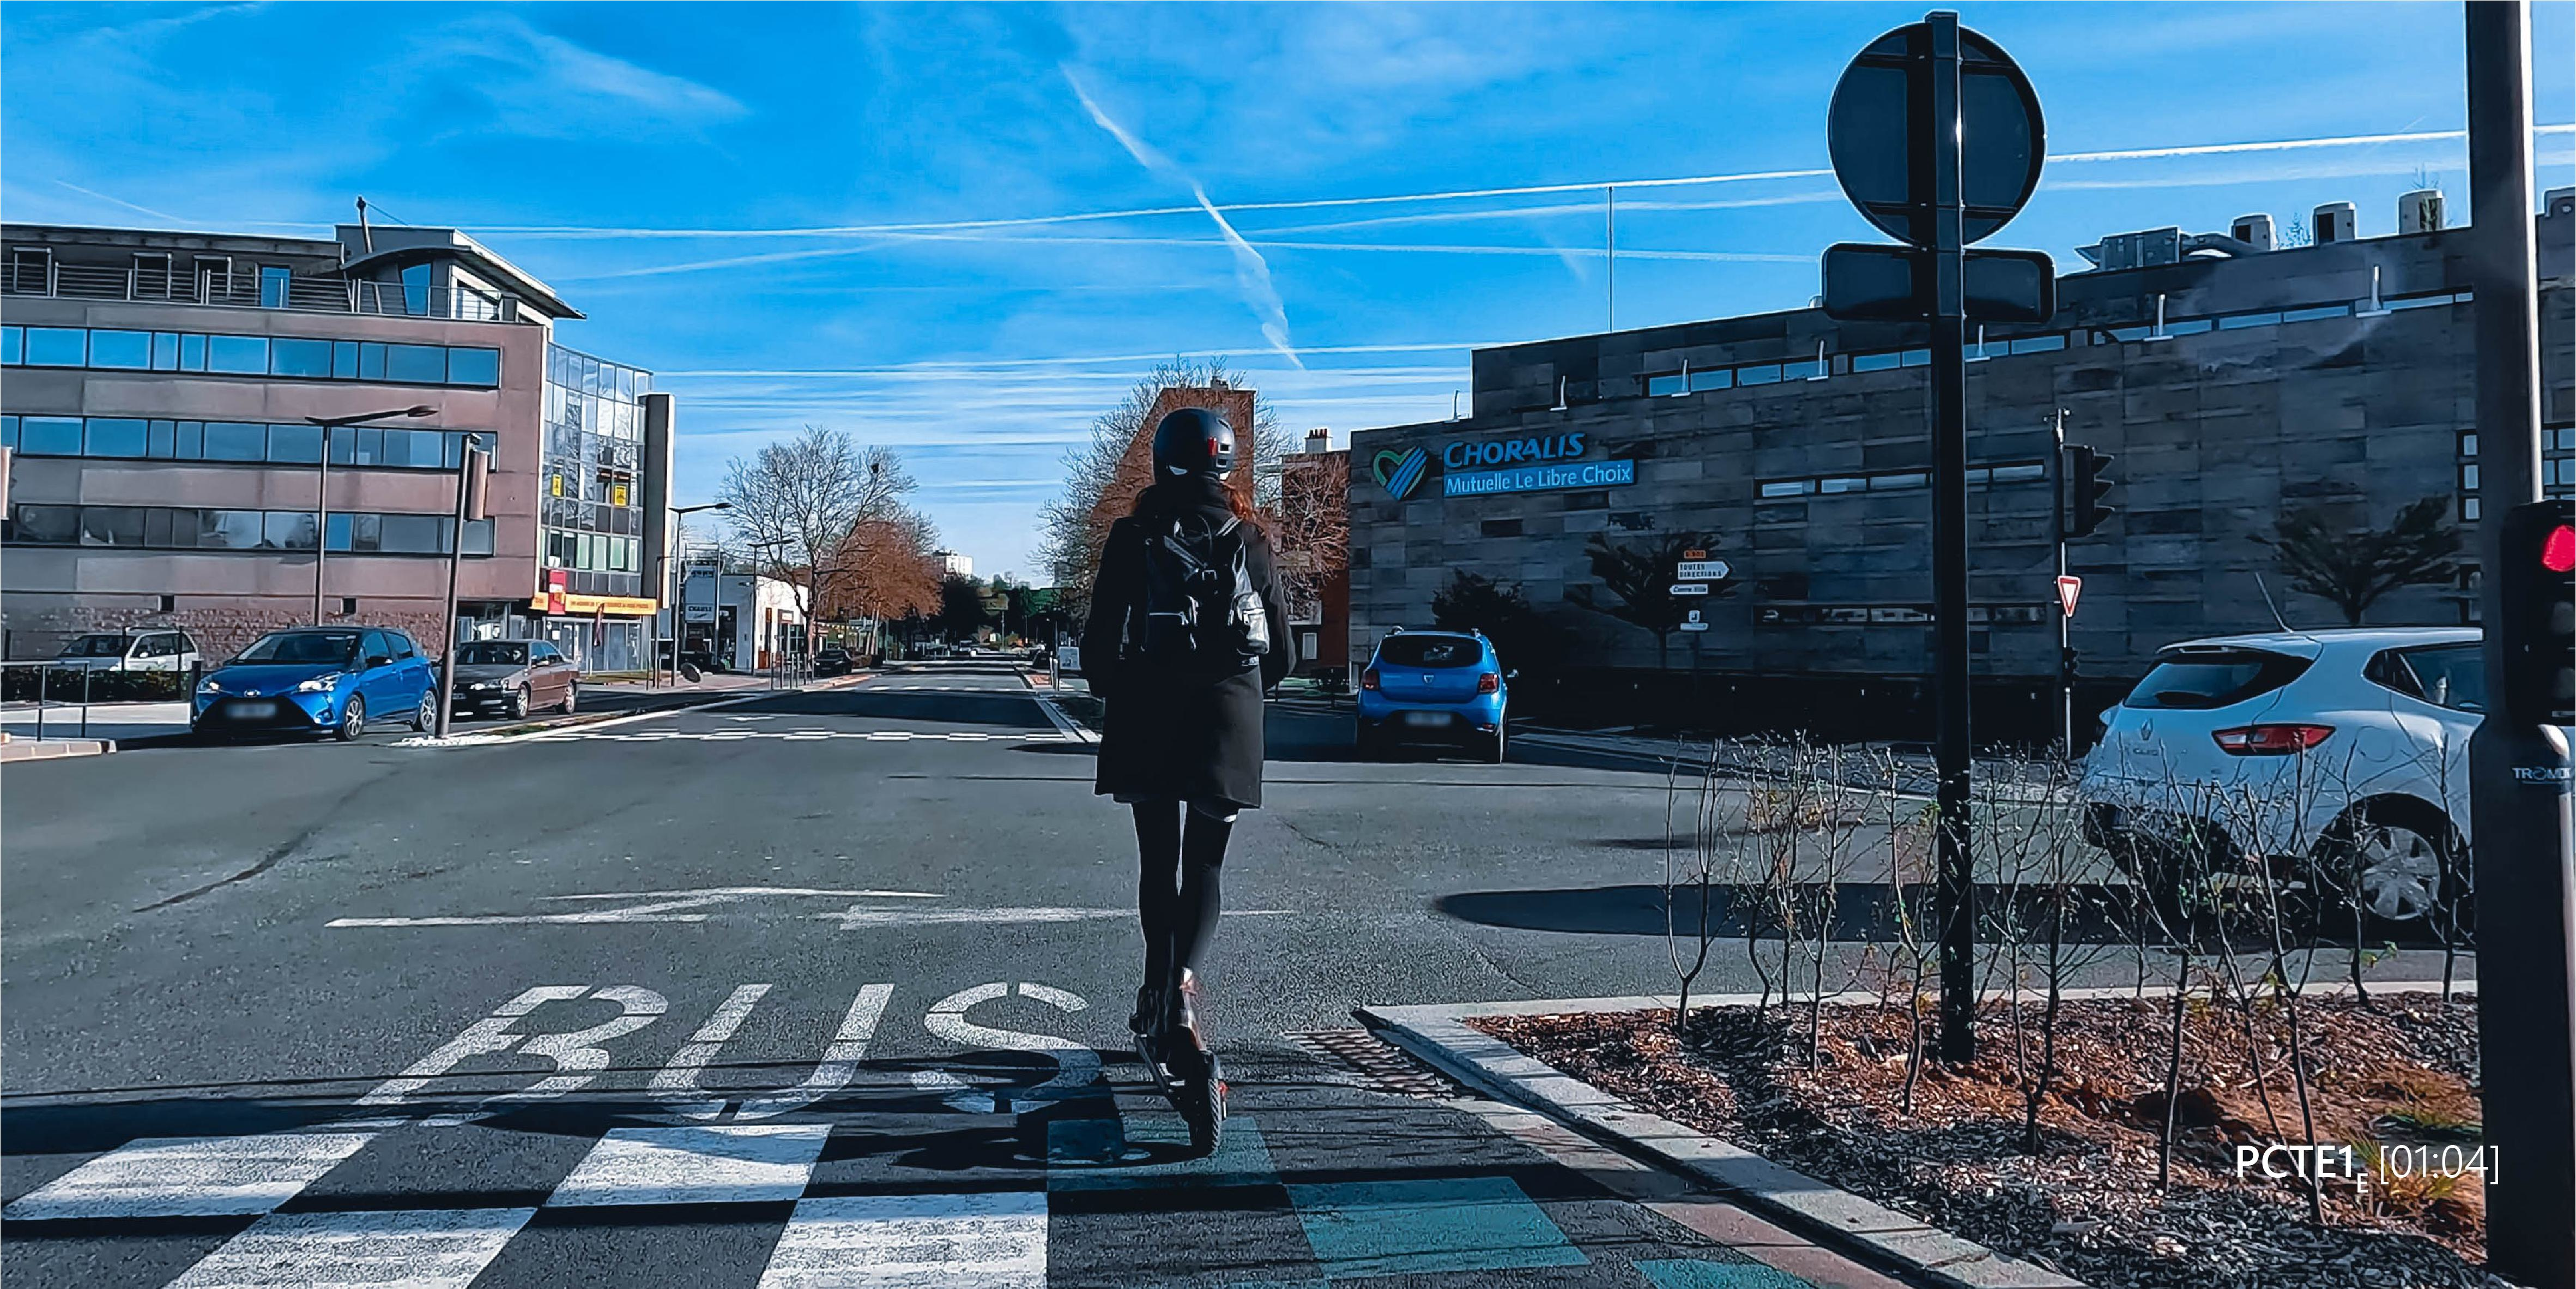
\includegraphics[width=0.75\columnwidth]{src/Figures/Annexes/Extrait_Video_PCTE1_Egress_3.jpg}}
        \vspace{5pt}
        \begin{flushright}\scriptsize{
        Author: \textcolor{blue}{Dylan Moinse (2022)}
        }\end{flushright}
    \end{figure}

    % PCTE1 Photo Egress 4
    \begin{figure}[h!]\vspace*{4pt}
        \caption*{Excerpt No. 4 from the video during the egress segment (\(PCTE^{E}_{1}\))}
        \centerline{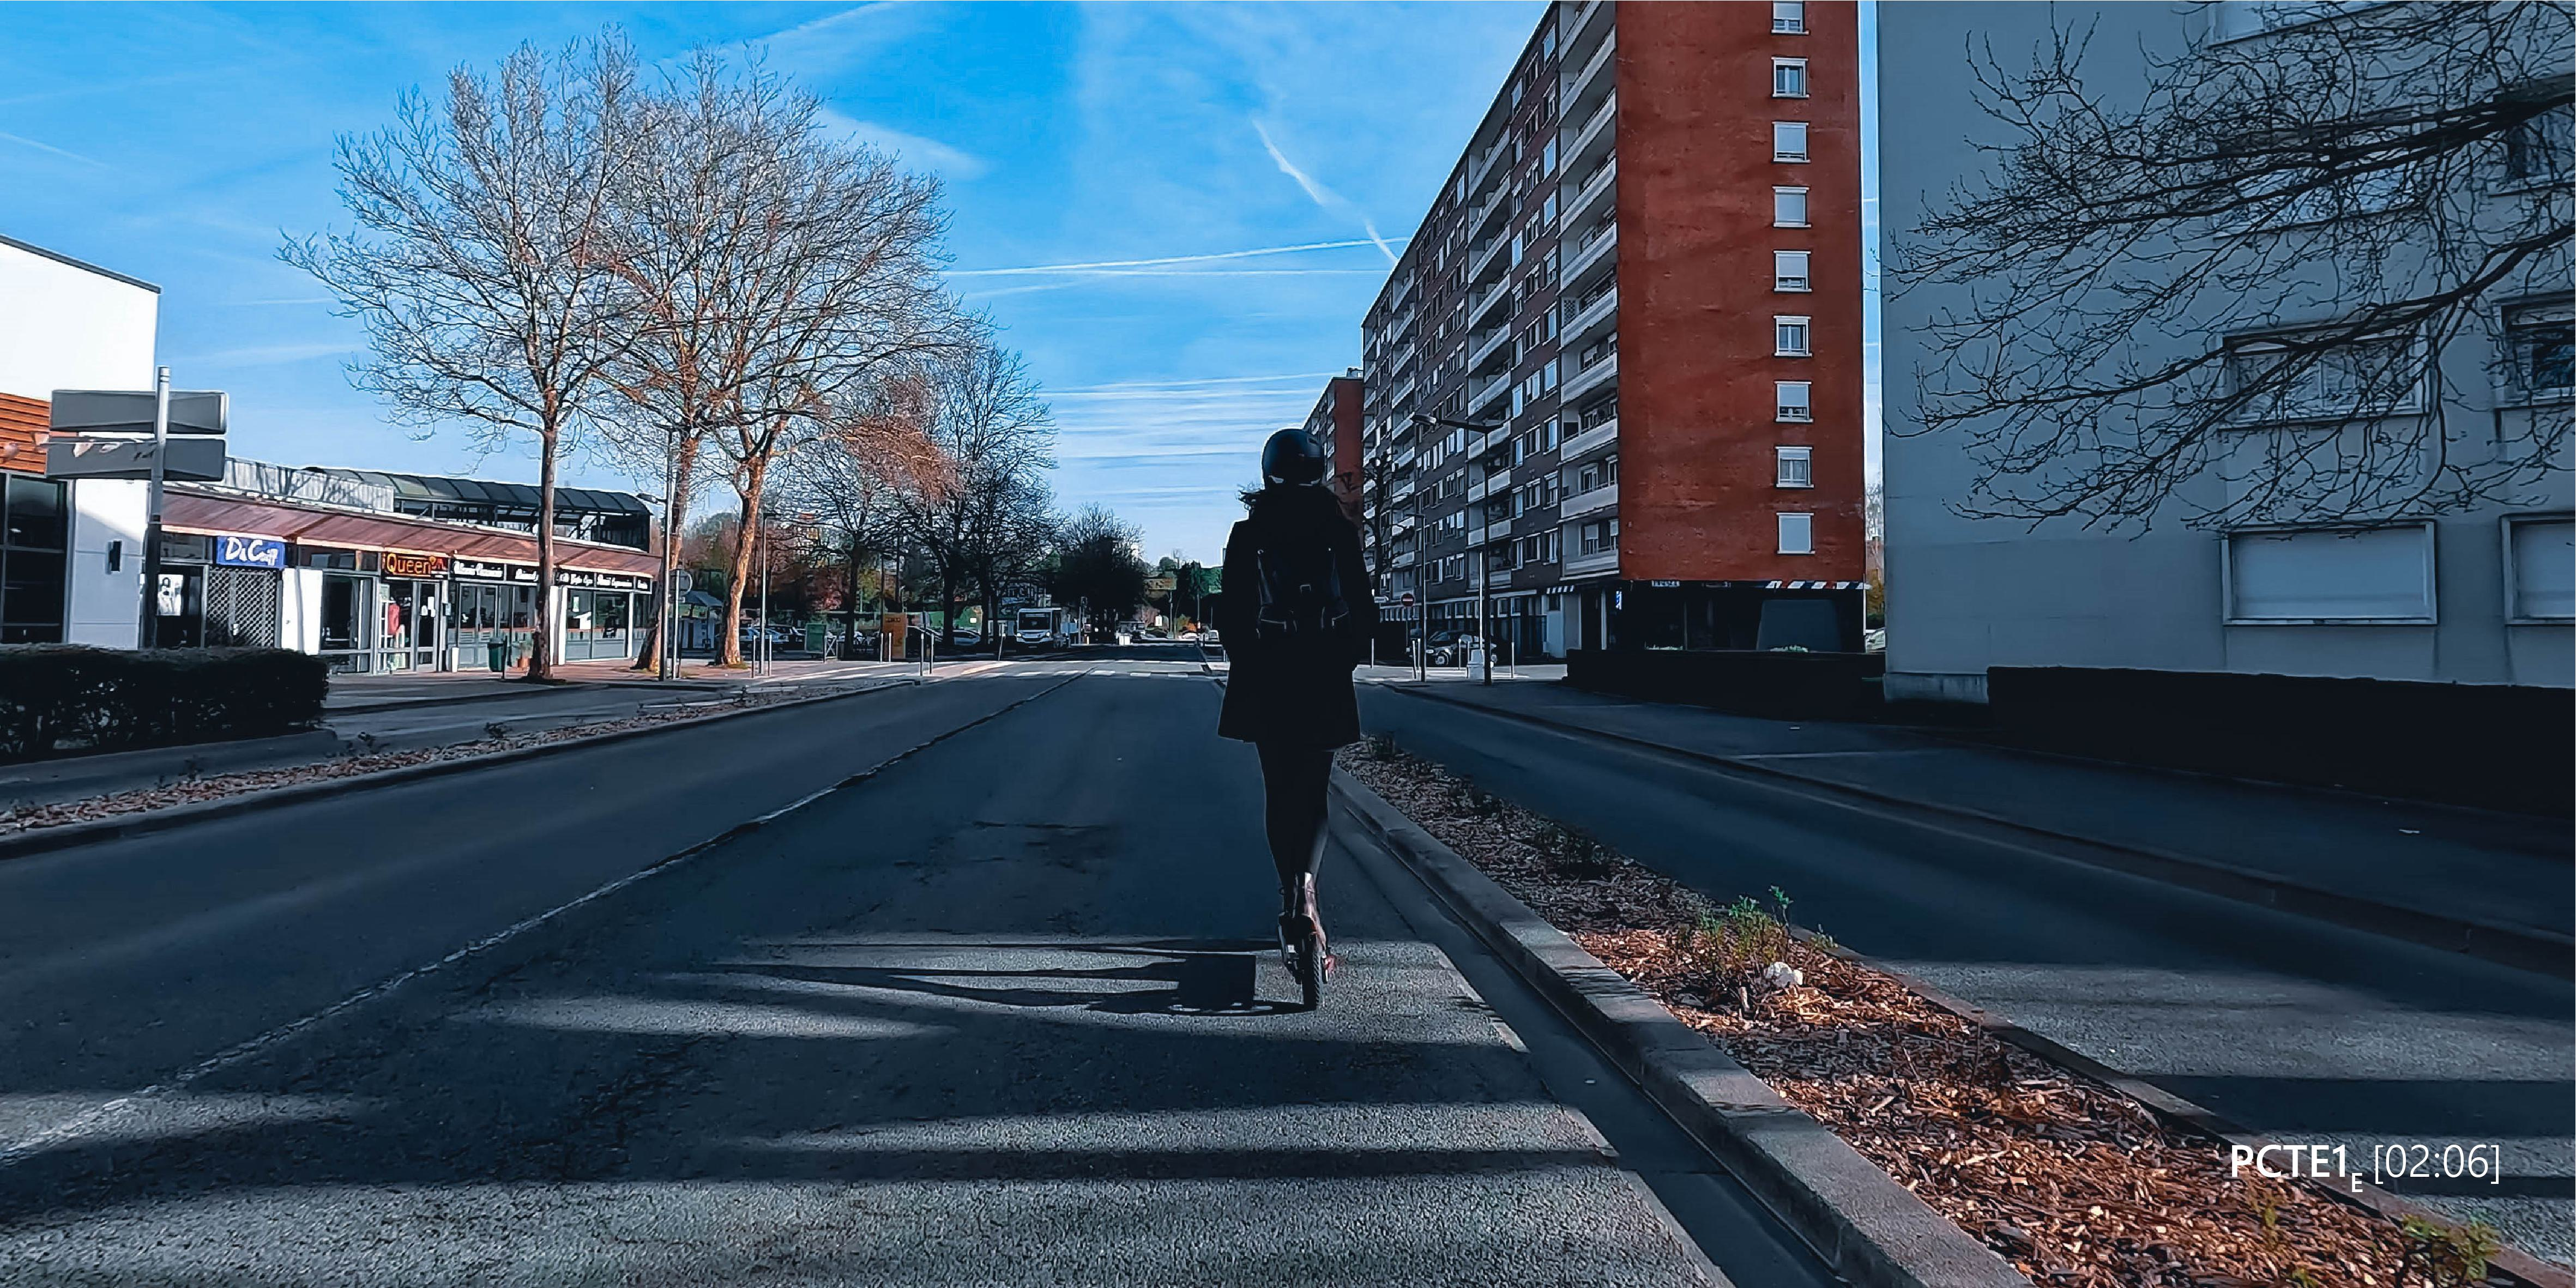
\includegraphics[width=0.75\columnwidth]{src/Figures/Annexes/Extrait_Video_PCTE1_Egress_4.jpg}}
        \vspace{5pt}
        \begin{flushright}\scriptsize{
        Author: \textcolor{blue}{Dylan Moinse (2022)}
        }\end{flushright}
    \end{figure}

    % PCTE1 Photo Egress 5
    \begin{figure}[h!]\vspace*{4pt}
        \caption*{Excerpt No. 5 from the video during the egress segment (\(PCTE^{E}_{1}\))}
        \centerline{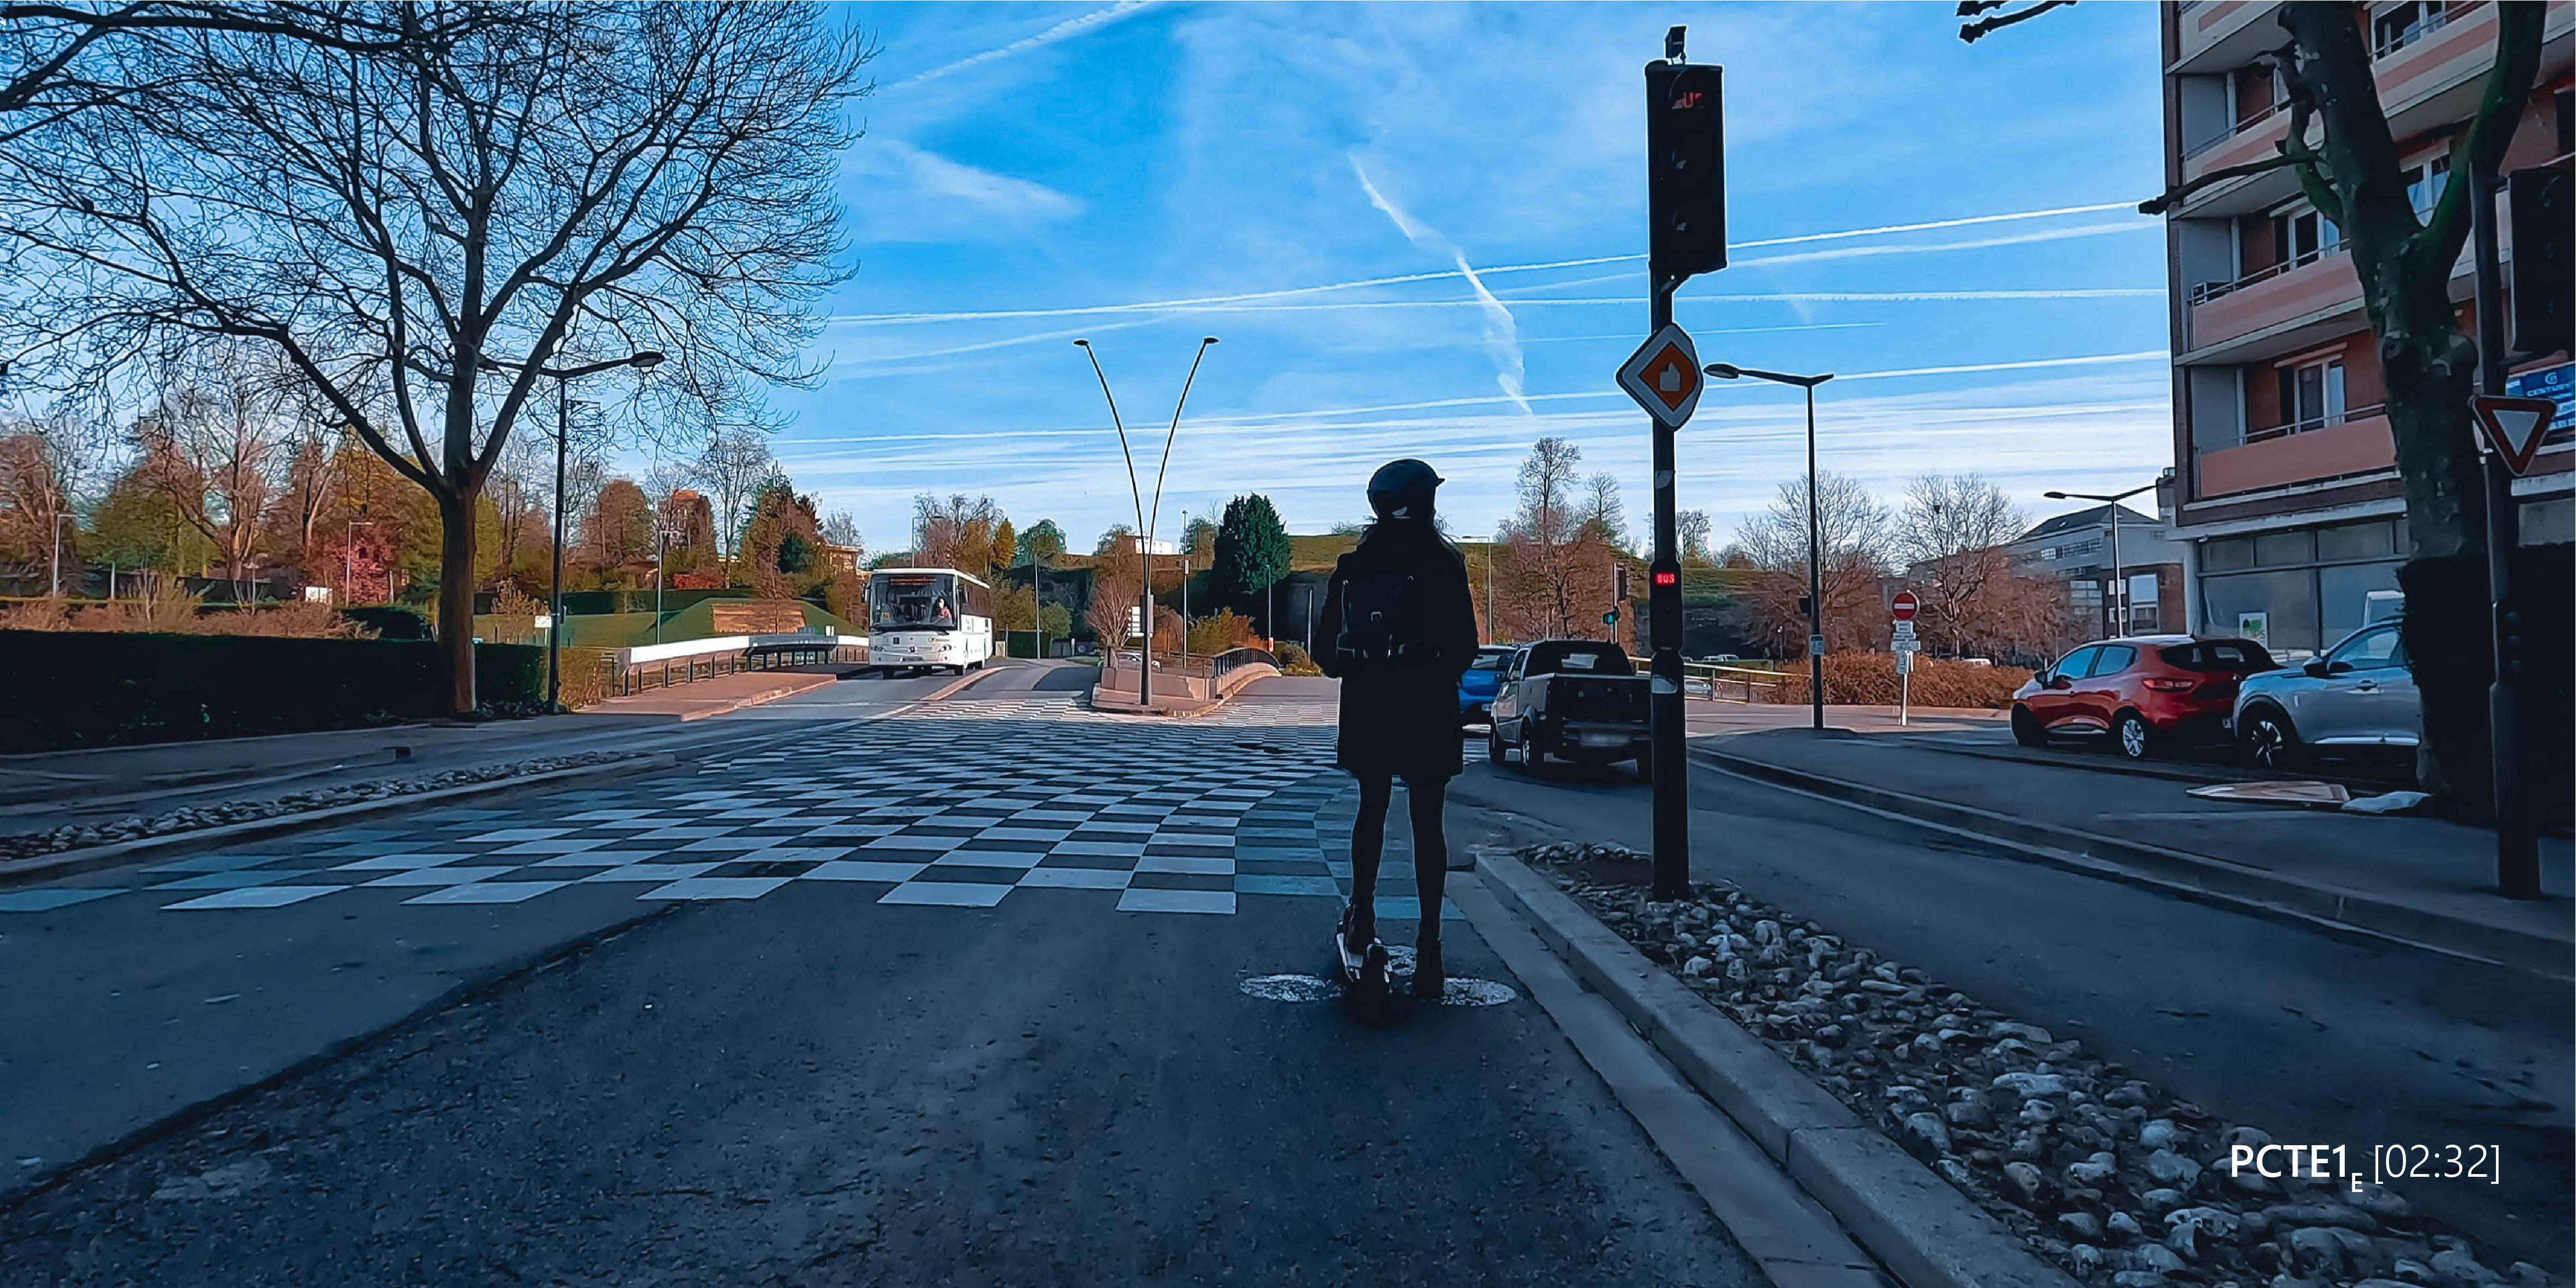
\includegraphics[width=0.75\columnwidth]{src/Figures/Annexes/Extrait_Video_PCTE1_Egress_5.jpg}}
        \vspace{5pt}
        \begin{flushright}\scriptsize{
        Author: \textcolor{blue}{Dylan Moinse (2022)}
        }\end{flushright}
    \end{figure}

    % PCTE1 Photo Egress 6
    \begin{figure}[h!]\vspace*{4pt}
        \caption*{Excerpt No. 6 from the video during the egress segment (\(PCTE^{E}_{1}\))}
        \centerline{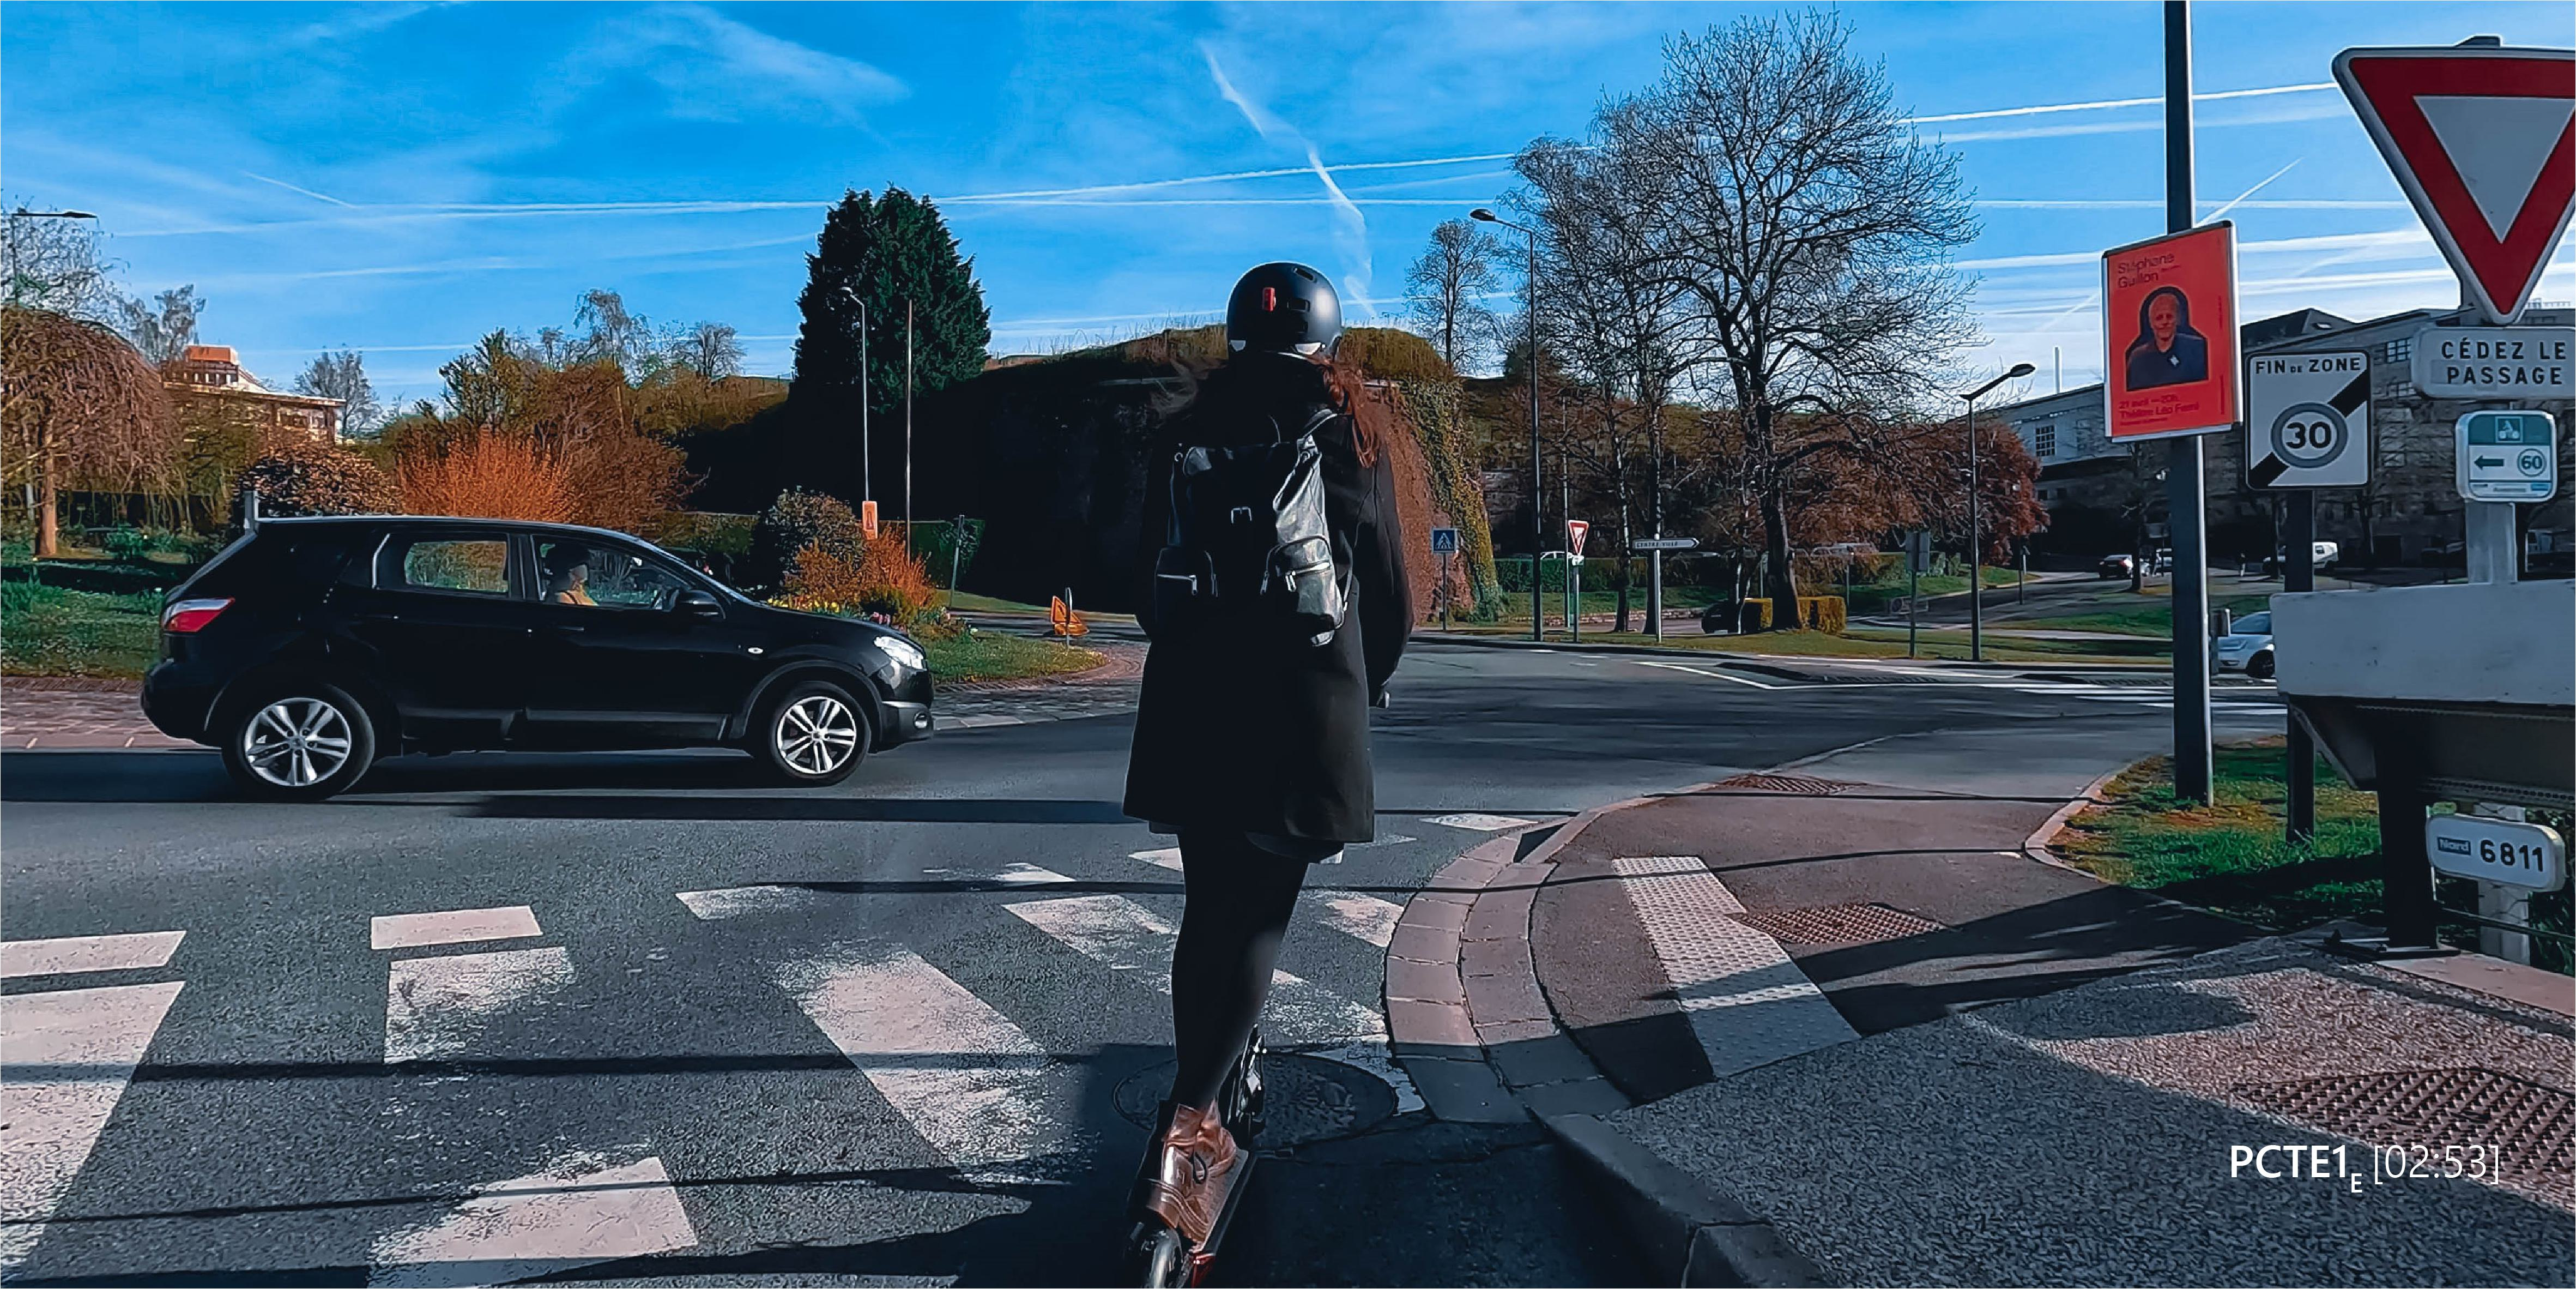
\includegraphics[width=0.75\columnwidth]{src/Figures/Annexes/Extrait_Video_PCTE1_Egress_6.jpg}}
        \vspace{5pt}
        \begin{flushright}\scriptsize{
        Author: \textcolor{blue}{Dylan Moinse (2022)}
        }\end{flushright}
    \end{figure}

    % PCTE1 Photo Egress 7
    \begin{figure}[h!]\vspace*{4pt}
        \caption*{Excerpt No. 7 from the video during the egress segment (\(PCTE^{E}_{1}\))}
        \centerline{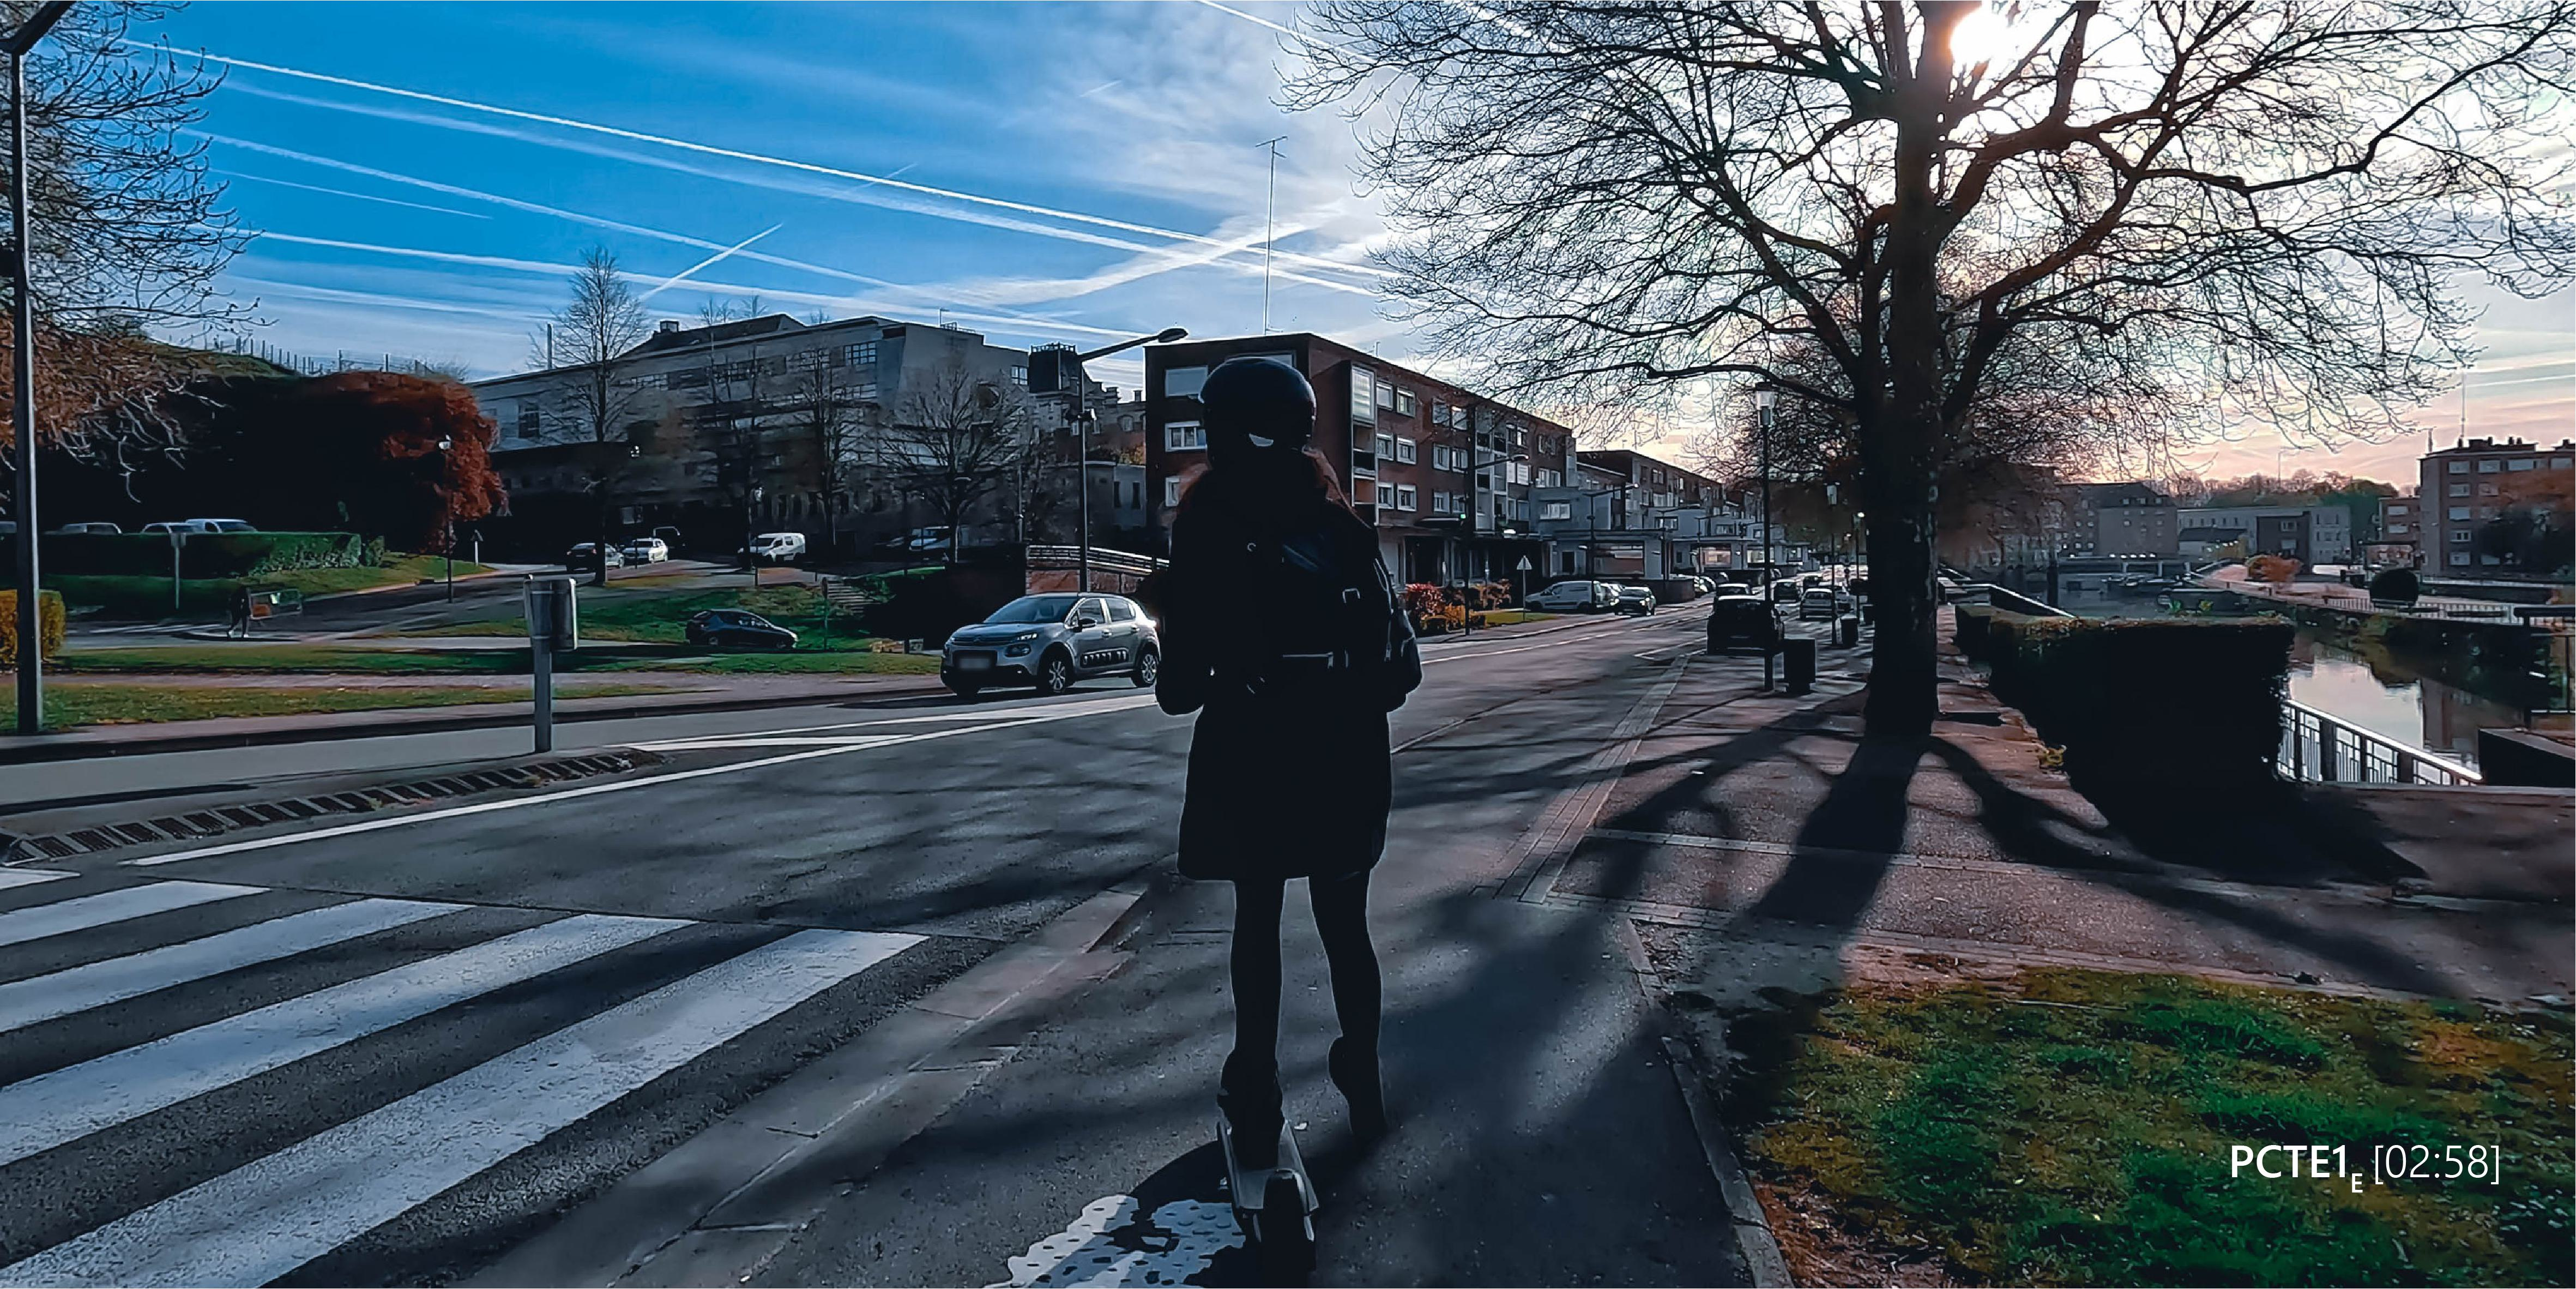
\includegraphics[width=0.75\columnwidth]{src/Figures/Annexes/Extrait_Video_PCTE1_Egress_7.jpg}}
        \vspace{5pt}
        \begin{flushright}\scriptsize{
        Author: \textcolor{blue}{Dylan Moinse (2022)}
        }\end{flushright}
    \end{figure}

    % PCTE1 Photo Egress 8
    \begin{figure}[h!]\vspace*{4pt}
        \caption*{Excerpt No. 8 from the video during the egress segment (\(PCTE^{E}_{1}\))}
        \centerline{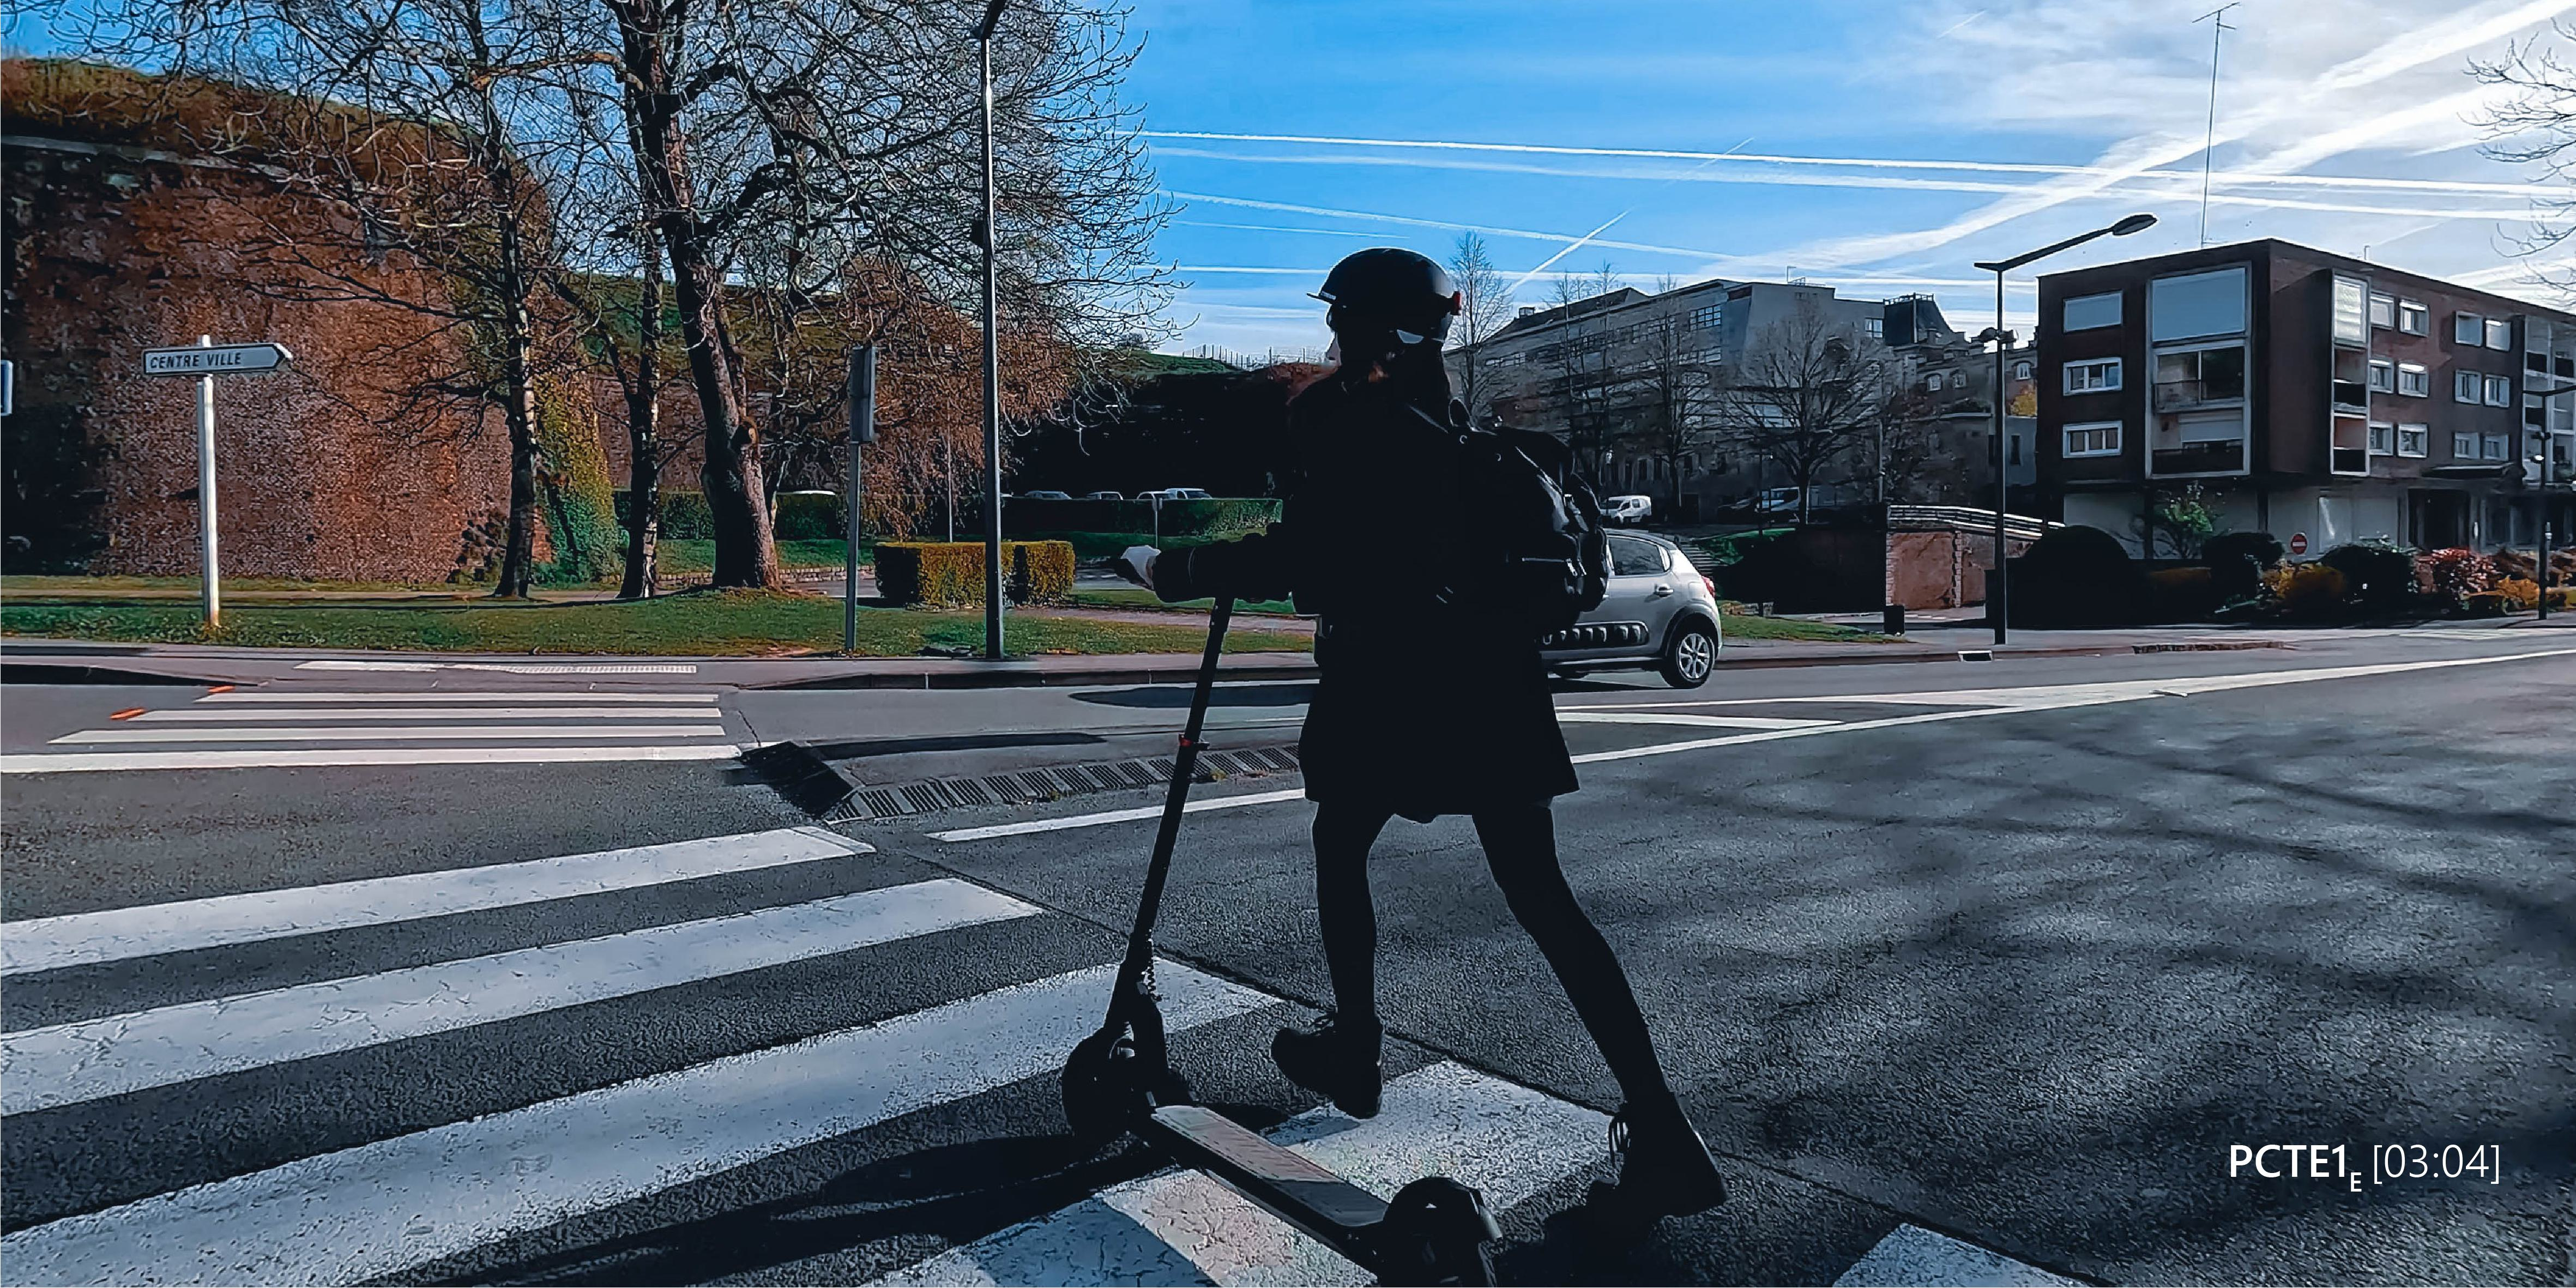
\includegraphics[width=0.75\columnwidth]{src/Figures/Annexes/Extrait_Video_PCTE1_Egress_8.jpg}}
        \vspace{5pt}
        \begin{flushright}\scriptsize{
        Author: \textcolor{blue}{Dylan Moinse (2022)}
        }\end{flushright}
    \end{figure}

    % PCTE1 Photo Egress 9
    \begin{figure}[h!]\vspace*{4pt}
        \caption*{Excerpt No. 9 from the video during the egress segment (\(PCTE^{E}_{1}\))}
        \centerline{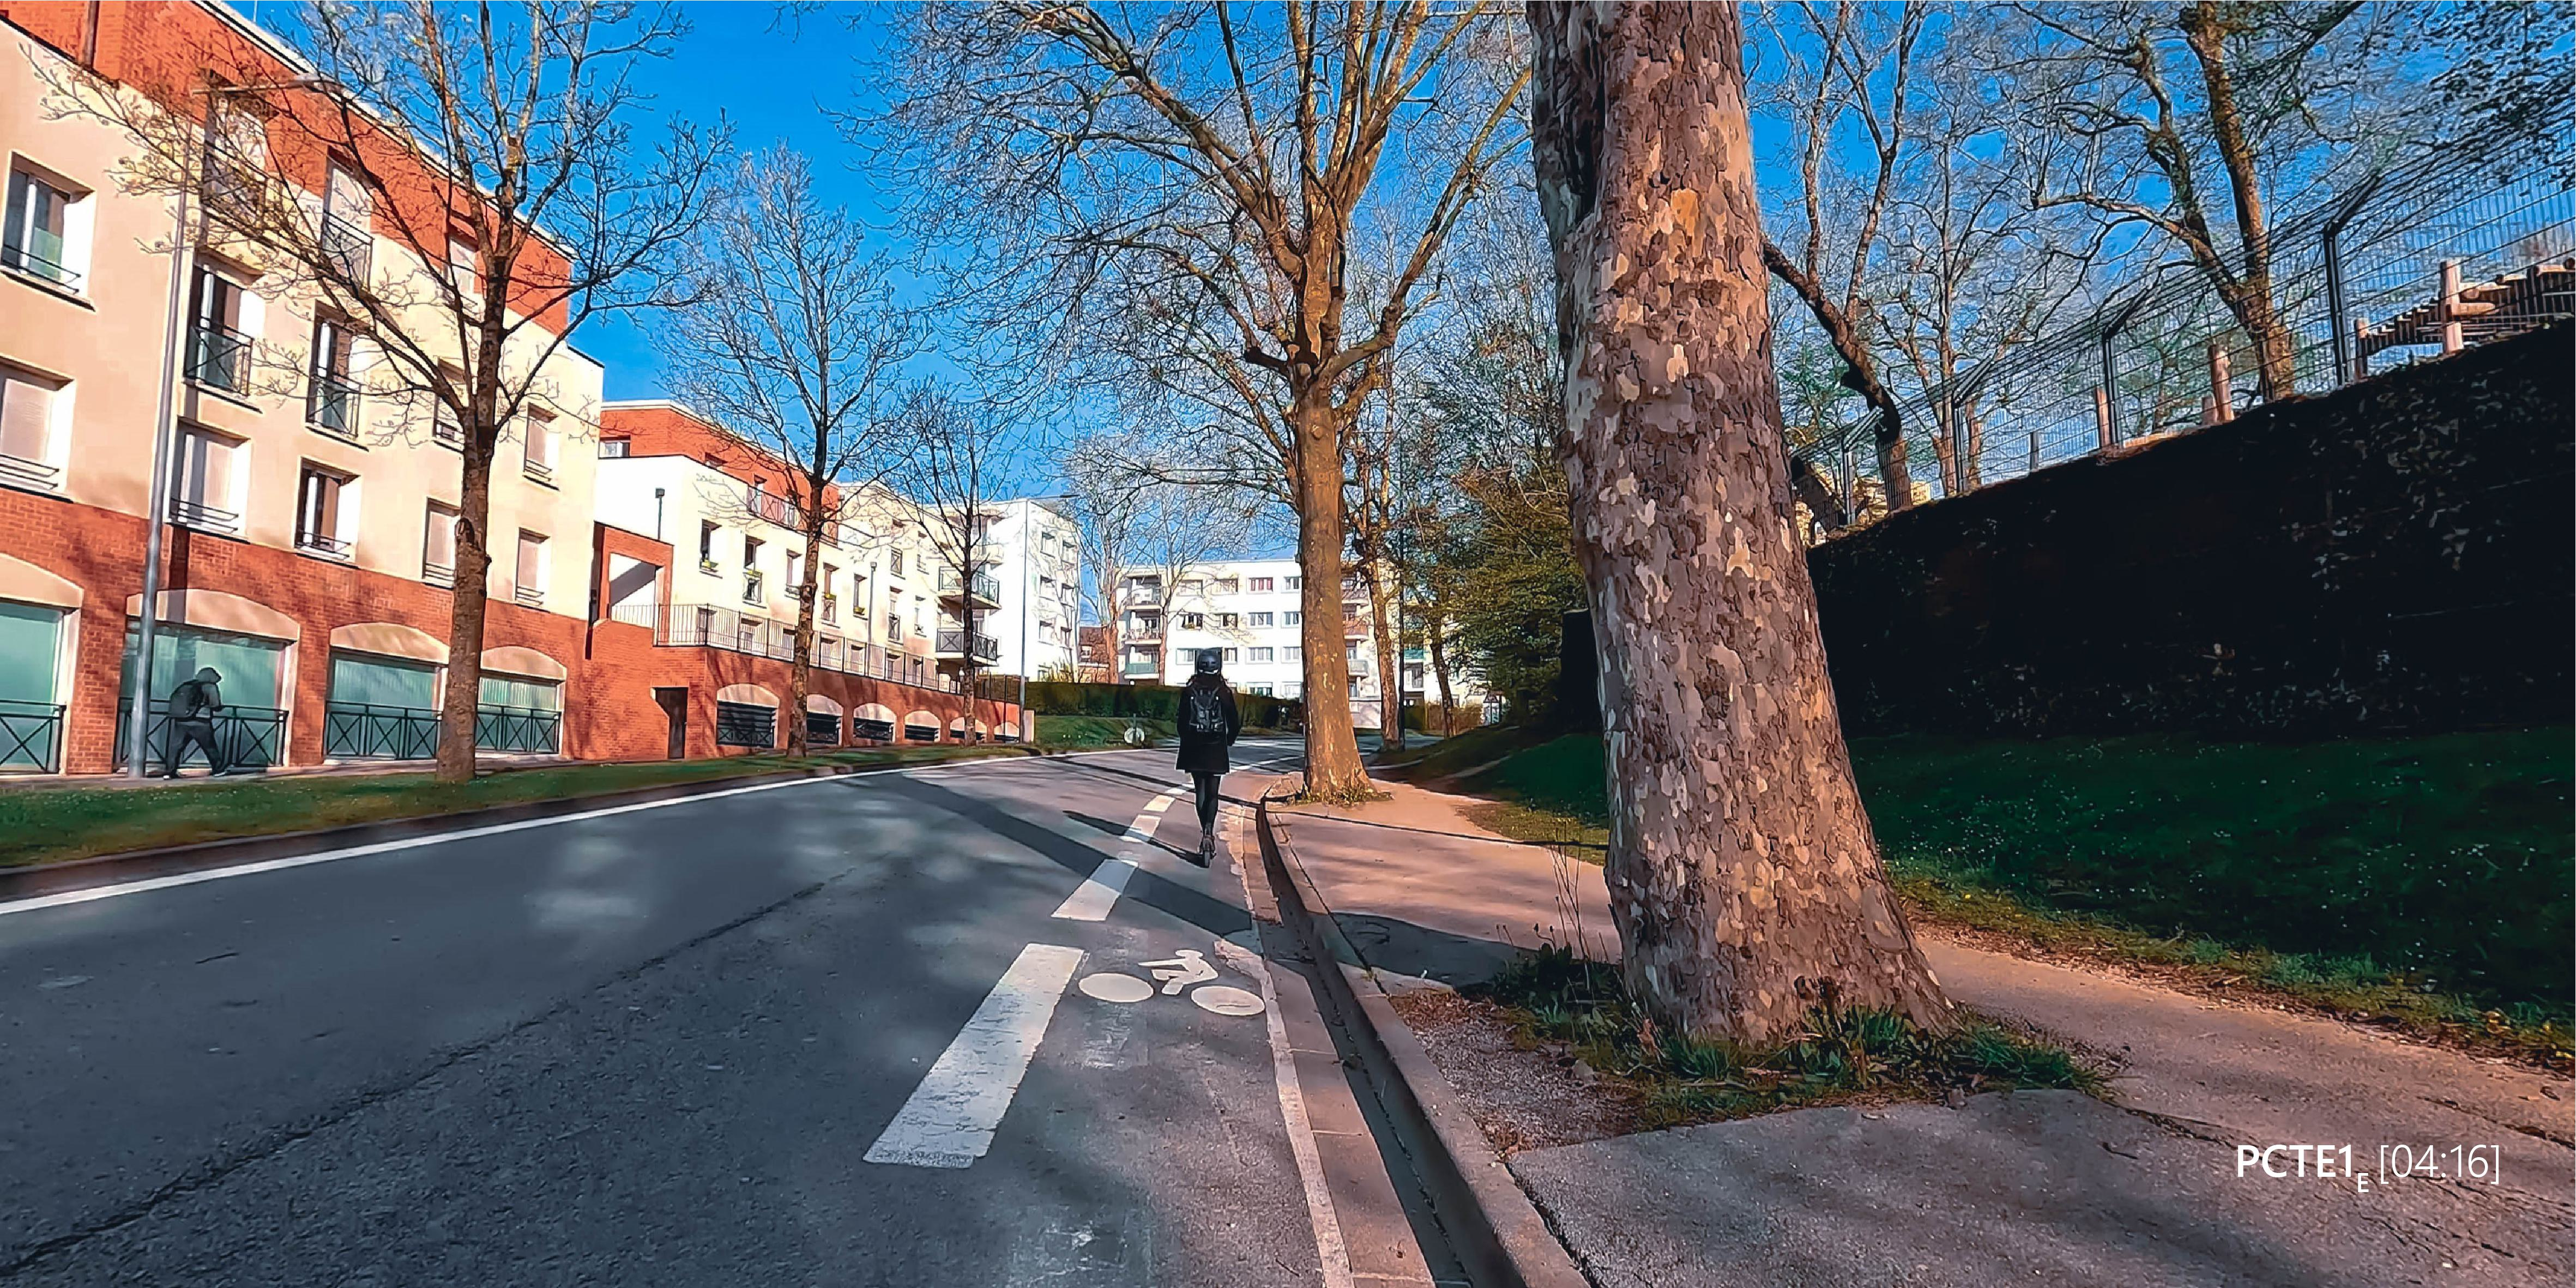
\includegraphics[width=0.75\columnwidth]{src/Figures/Annexes/Extrait_Video_PCTE1_Egress_9.jpg}}
        \vspace{5pt}
        \begin{flushright}\scriptsize{
        Author: \textcolor{blue}{Dylan Moinse (2022)}
        }\end{flushright}
    \end{figure}

    % PCTE1 Photo Egress 10
    \begin{figure}[h!]\vspace*{4pt}
        \caption*{Excerpt No. 10 from the video during the egress segment (\(PCTE^{E}_{1}\))}
        \centerline{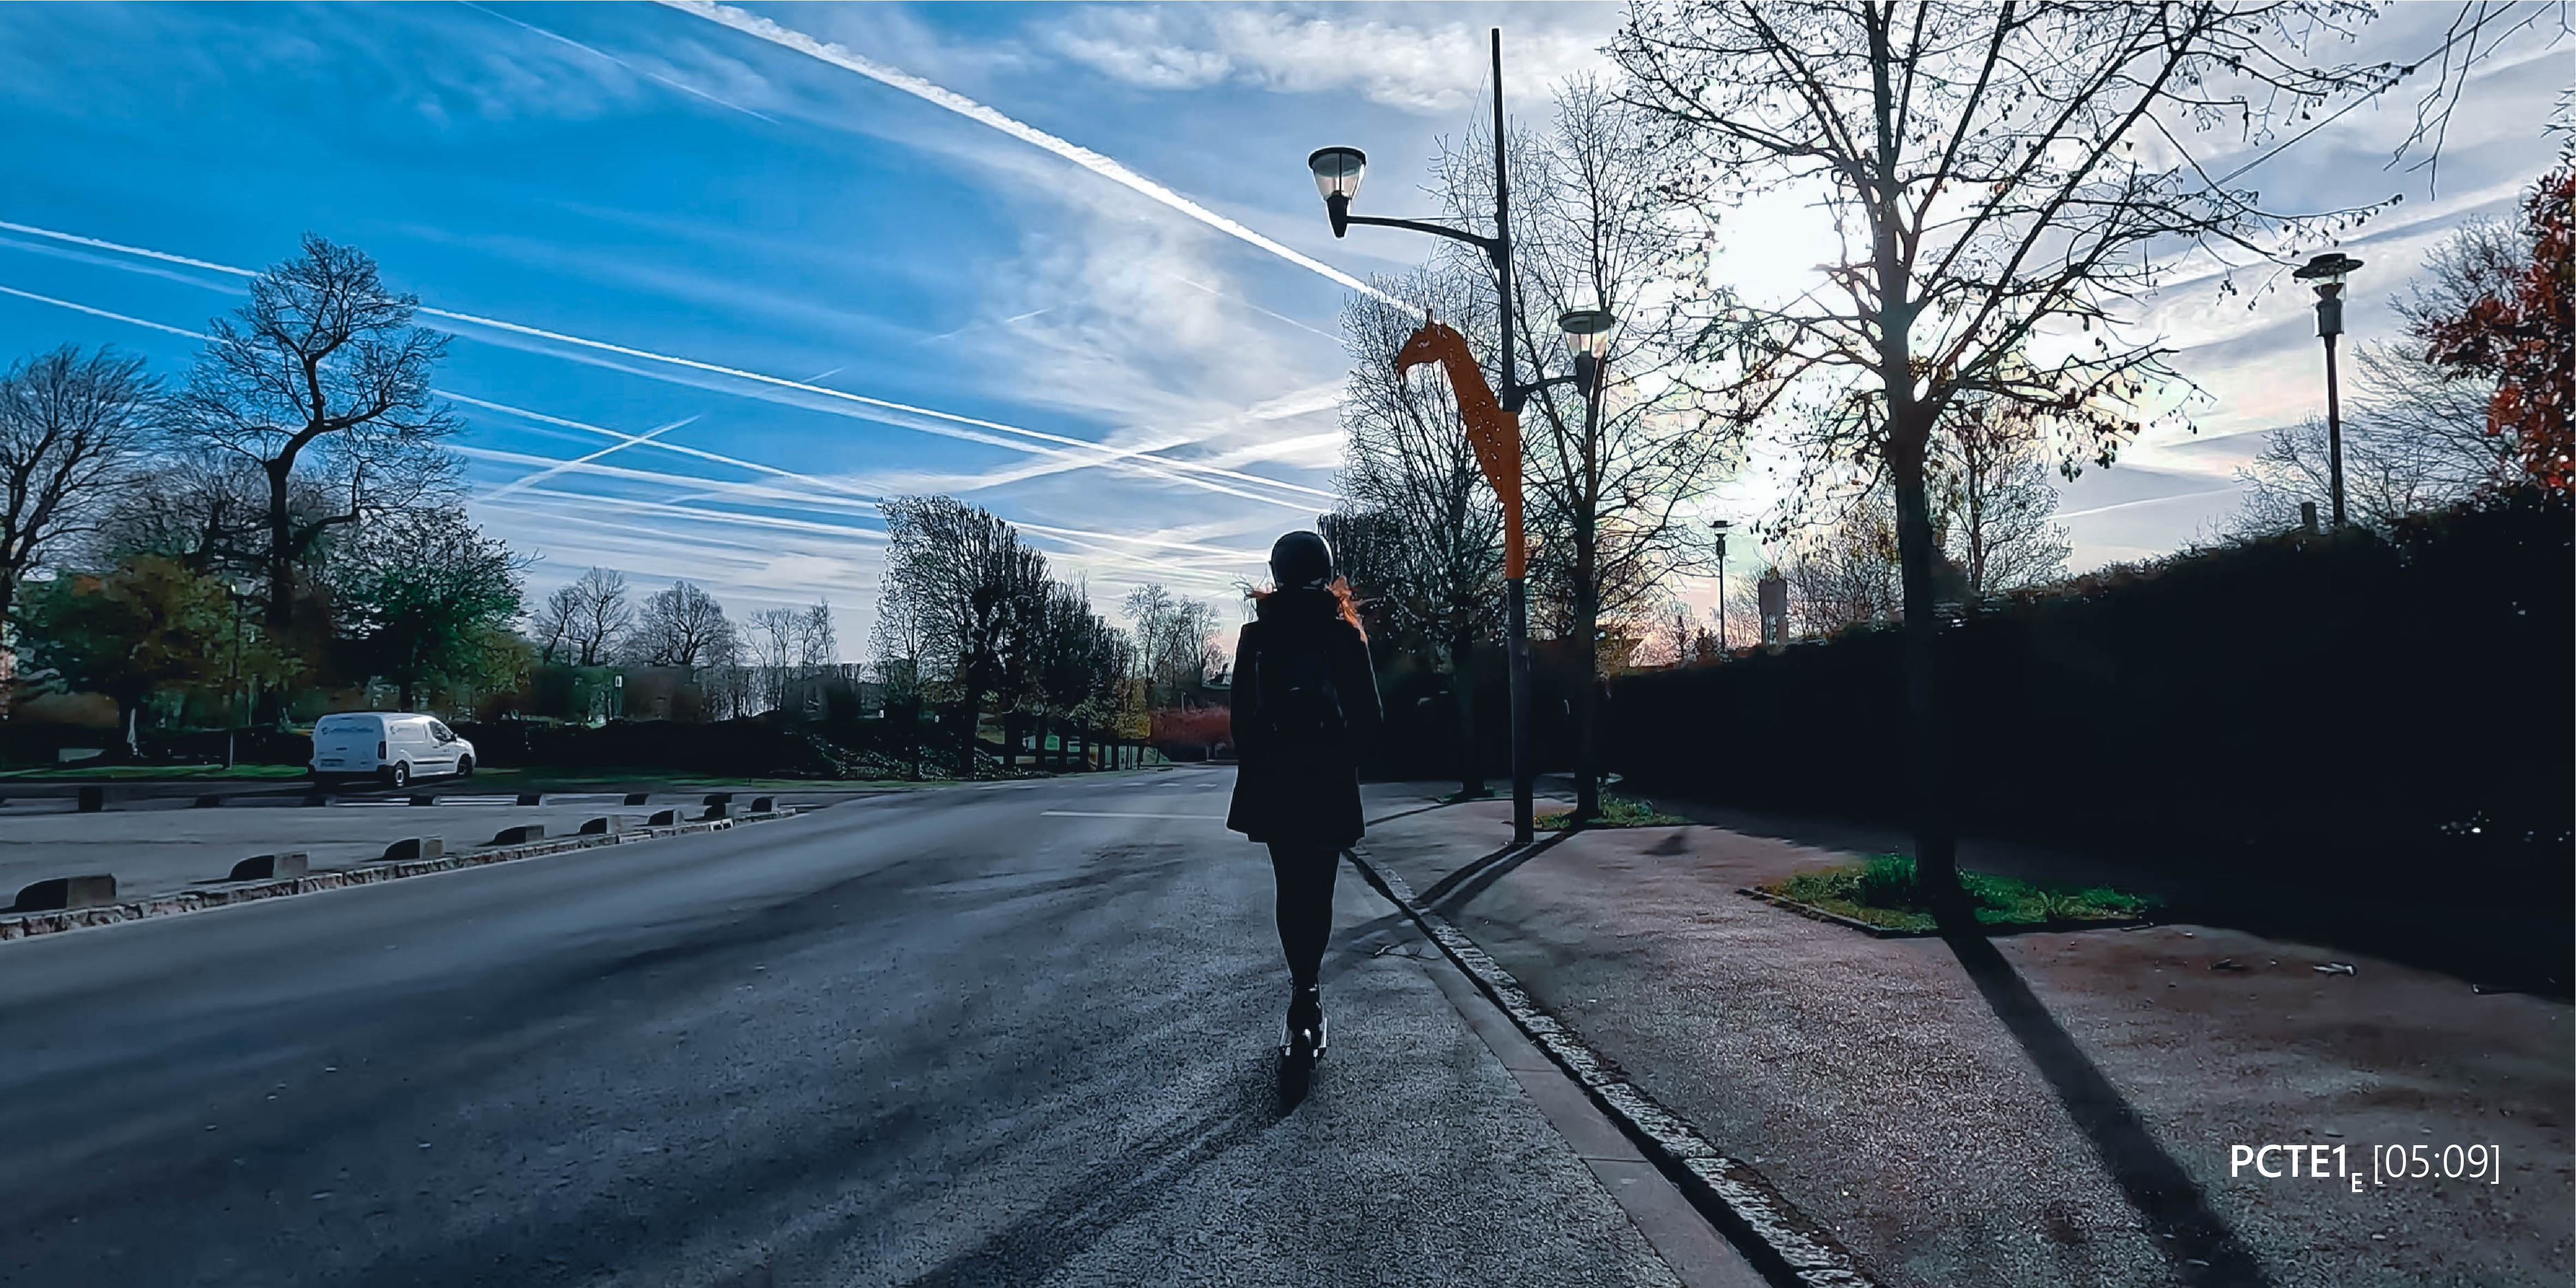
\includegraphics[width=0.75\columnwidth]{src/Figures/Annexes/Extrait_Video_PCTE1_Egress_10.jpg}}
        \vspace{5pt}
        \begin{flushright}\scriptsize{
        Author: \textcolor{blue}{Dylan Moinse (2022)}
        }\end{flushright}
    \end{figure}

    % Retranscription PCTE2
    \newpage
    \needspace{1\baselineskip} % Reserve space
    \sectionheader{Transcription of the Second Ride-Along Interview}
\section{Transcription of the Second Ride-Along Interview}
    \label{annexes:retranscription-pcte2}

    % Retranscription PCTE2 detour
\subsection{Transcribed Exchanges During the Access Trip by e-Scooter}

\begin{description}
    \item[Participant \(PCTE^{A}_{2}\)] [00:27]: Here, I’m going straight ahead because if I turn right, I’ll \textsl{hit} a street with cobblestones. A bike lane [instead of parking spaces] would be enough in this street, since it’s not very busy.
    \item[Participant \(PCTE^{A}_{2}\)] [00:58]: On a \textsl{V'Lille}, cobblestones bother me less, but here\dots \textsl{No}\dots not on a scooter.
    \item[Participant \(PCTE^{A}_{2}\)] [02:00]: It doesn’t bother me that much to ride alongside cars, you see. However, I end up squeezed between parked cars on the side of the road, and I’m always afraid of getting hit by an opening car door.
    \item[Participant \(PCTE^{A}_{2}\)] [02:44]: On the way back, I’m not satisfied with the contra-flow bike lanes [the two-way bike lane], because there are always cars parked poorly. It’s stressful when you cross a car, because you need space to pass it. Often, I stop in front of a car.
    \item[Participant \(PCTE^{A}_{2}\)] [03:15]: Now, I’m going onto the bike box. It’s useful for turning left. You’re not stuck between the cars.
    \item[Participant \(PCTE^{A}_{2}\)] [04:45]: \textsl{Here}, there are a lot of driveways in this street and people don’t pay much attention. I don’t like bike lanes next to parked cars because of the doors. And at the end of the street, you don’t know what to do. For me, coming to the metro, I have to go straight ahead across the crosswalk and onto the sidewalk.%%Translated%%
\end{description}

    % Retranscription PCTE2 TC
\subsection{Transcribed Exchanges During the Metro Trip}

\begin{description}
    \item[Participant \(PCTE^{TC}_{2}\)] [00:03]: \textsl{Hop!} The escalators are good because they save me from carrying the weight of the scooter up the stairs. But it’s not optimal, because I have to find the right grip for the scooter. I don’t take the metro elevator because it’s generally for people with reduced mobility [PRM], and because it’s \textsl{sketchy}.
    \item[Participant \(PCTE^{TC}_{2}\)] [03:29]: I have to stay in the central square of the metro because there’s no space elsewhere. If I sit, there’s no room for my scooter. So, I stand with my scooter. I also prefer being in this central space because if I were by the door, I’d have to move every time it opens.%%Translated%%
    
    Ideally, I wedge my route against the metro bar and hold on to the handlebar to stay steady in the metro. It’s the best technique I’ve got, because you can’t really place it without it falling and disturbing everyone. At least, I bother people less this way, I think.%%Translated%%

    \item[Participant \(PCTE^{TC}_{2}\)] [04:20]: I specifically chose a scooter that’s not too heavy, so I can carry it easily in places where I can’t ride, like stairs or in the metro.
    \item[Participant \(PCTE^{TC}_{2}\)] [04:39]: Since I have flexible hours, I go earlier to avoid rush hours, because otherwise there’s no room to ride the scooter.
    \item[Participant \(PCTE^{TC}_{2}\)] [05:02]: When we get to my main building, which is my office, building \textsl{X} and the other \textsl{Y} where I work and often have classes.
    \item[Investigator] [05:20]: So, occasionally, you go to another building on campus using your electric scooter?
    \item[Participant \(PCTE^{TC}_{2}\)] [05:25]: That’s right. At least once a week, often twice.
    \item[Investigator] [05:32]: Can you explain in more detail the journey you make by scooter and metro?
    \item[Participant \(PCTE^{TC}_{2}\)] [05:35]: \textsl{Basically}, I always go to \textsl{X} to pick up my things, like my lab coat, my computer, \textsl{and all}. Then, I go to \textsl{Y}. It’s pleasant to ride the scooter around campus.
    \item[Investigator] [06:02]: Can you describe what you mean by \textsl{pleasant}?
    \item[Participant \(PCTE^{TC}_{2}\)] [06:09]: It’s generally calm. \textsl{But at the same time\dots No.} There’s no designated space for bikes and scooters on campus. But it’s true that we are quickly limited because we never know where to go. As soon as we go on the road, between the cars parked on the side and the narrow streets, we quickly feel oppressed by the cars behind us. It’s true that we also have to dodge pedestrians.
    \item[Investigator] [07:26]: And why not take the metro to go from \textsl{X} to \textsl{Y}?
    \item[Participant \(PCTE^{TC}_{2}\)] [07:38]: In this case, it would be quicker to walk there. To go to the metro, I would have to go back to \textsl{Cité Scientifique} [the arrival station], wait for the metro, and go to \textsl{4 Cantons} [the terminus of Line 1] to walk after. Whereas here, I quickly cross the campus. On the scooter, it takes me less than five minutes, while on foot, it’s at least twenty minutes. Especially since I then have to do the return, so that’s double.
    \item[Investigator] [08:05]: So, for you, the metro is efficient for long distances, like the journey between \textsl{République - Beaux-Arts} and \textsl{Cité Scientifique}. But, it’s less interesting when you face short distances, but not short enough to walk, and you prefer to take the scooter?
    \item[Participant \(PCTE^{TC}_{2}\)] [08:20]: Short distances, with buildings that aren’t next to the metro stations. If my two buildings were next to the two metro stops, I would have taken the metro. Here, it’s during my work, I can’t afford to lose forty minutes walking. On the scooter, for a round trip, I save more than thirty minutes. Honestly, I would take the car if I had to walk that much, it would be simpler. And still, I easily make several round trips [between \textsl{X} and \textsl{Y}] in a day\dots [We arrive at the destination, at the \textsl{Cité Scientifique Pr. Gabillard} stop.]%%Translated%%

    Afterward, the scooter is not very practical. Because of the fences, I ride on the sidewalks because we don’t have access to the campus roads.
    \item[Investigator] [08:38]: We can continue the conversation on the scooter, but before, I need to end this audio interview. Do you have any comments or questions?
    \item[Participant \(PCTE^{TC}_{2}\)] [08:44]: Everything’s fine for me.%%Translated%%
\end{description}

    % Entretien en Egress
\subsection{Transcribed Exchanges During the Egress Trip by e-Scooter}

\begin{description}
    \item[Participant \(PCTE^{E}_{2}\)] [00:47]: I have to keep my scooter folded when I exit the metro to pass through the turnstile. I have to push \textsl{all the way} against the door, because it doesn’t detect my scooter. So, it doesn’t open.%%Translated%%

    The turnstiles are not wide enough for me to walk beside my scooter. And I don’t know how the turnstile works for people with reduced mobility.%%Translated%%

    It was better before, when there was no turnstile. It was more fluid. And for the reasons mentioned. There are two turnstiles for an extremely busy metro station.
    \item[Participant \(PCTE^{E}_{2}\)] [02:03]: Now that we’ve arrived at \textsl{Cité Scientifique} [the arrival station], I have two possible paths to choose from. I can either go by the road or through the buildings [the pedestrian pathways within the campus]. I prefer going through the buildings because the road is more pleasant. The road on campus is not suitable for cyclists and \textsl{scootists} [points to Avenue Paul Langevin that surrounds the campus].
    \item[Participant \(PCTE^{E}_{2}\)] [03:13]: These are new paths that have just been built, and they’re pleasant. They’ve been here for five or six months, I would say.
    \item[Participant \(PCTE^{E}_{2}\)] [03:19]: I have to dodge pedestrians though, \textsl{it’s annoying.}
    \item[Participant \(PCTE^{E}_{2}\)] [03:29]: \textsl{Here}, we’re going on a one-way street\dots \textsl{We do what we can, huh.} It’s rare to see one-way streets, even for bikes. There’s plenty of space on campus. If you can show \textsl{over there}, with the camera, the one-way sign. You can see there’s space for cars and space for\dots \textsl{who knows what.}%%Translated%%

    It could definitely be a bike lane. But, I avoid using this one-way road to get to building \textsl{Y} because there are some really unpleasant speed bumps for \textsl{scootists}. I prefer to go this way [a parallel pathway] even if I have to get off the scooter at one point. It’s still more pleasant.
    \item[Participant \(PCTE^{E}_{2}\)] [06:47]: This road is \textsl{terrible.} We don’t know \textsl{where} the sidewalk is and \textsl{where} the road is. Because of the zigzags, I often go on the sidewalk. Otherwise, I have to wait for the car coming from the other direction to pass. Since the sidewalk is wide, I don’t know if it’s shared [between pedestrians and cyclists].%%Translated%%
\end{description}

    % Photos PCTE2
    \newpage
\subsection{Selection of Images Extracted from the Second Ride-Along Interview}
    \label{annexes:photos-pcte2}

    % Photos PCTE2 detour
\subsubsection{Selection of Images Extracted During the Access Trip}

    % PCTE2 Photo Access 1
    \begin{figure}[h!]\vspace*{4pt}
        \caption*{Excerpt No. 1 from the video during the access segment (\(PCTE^{A}_{2}\))}
        \centerline{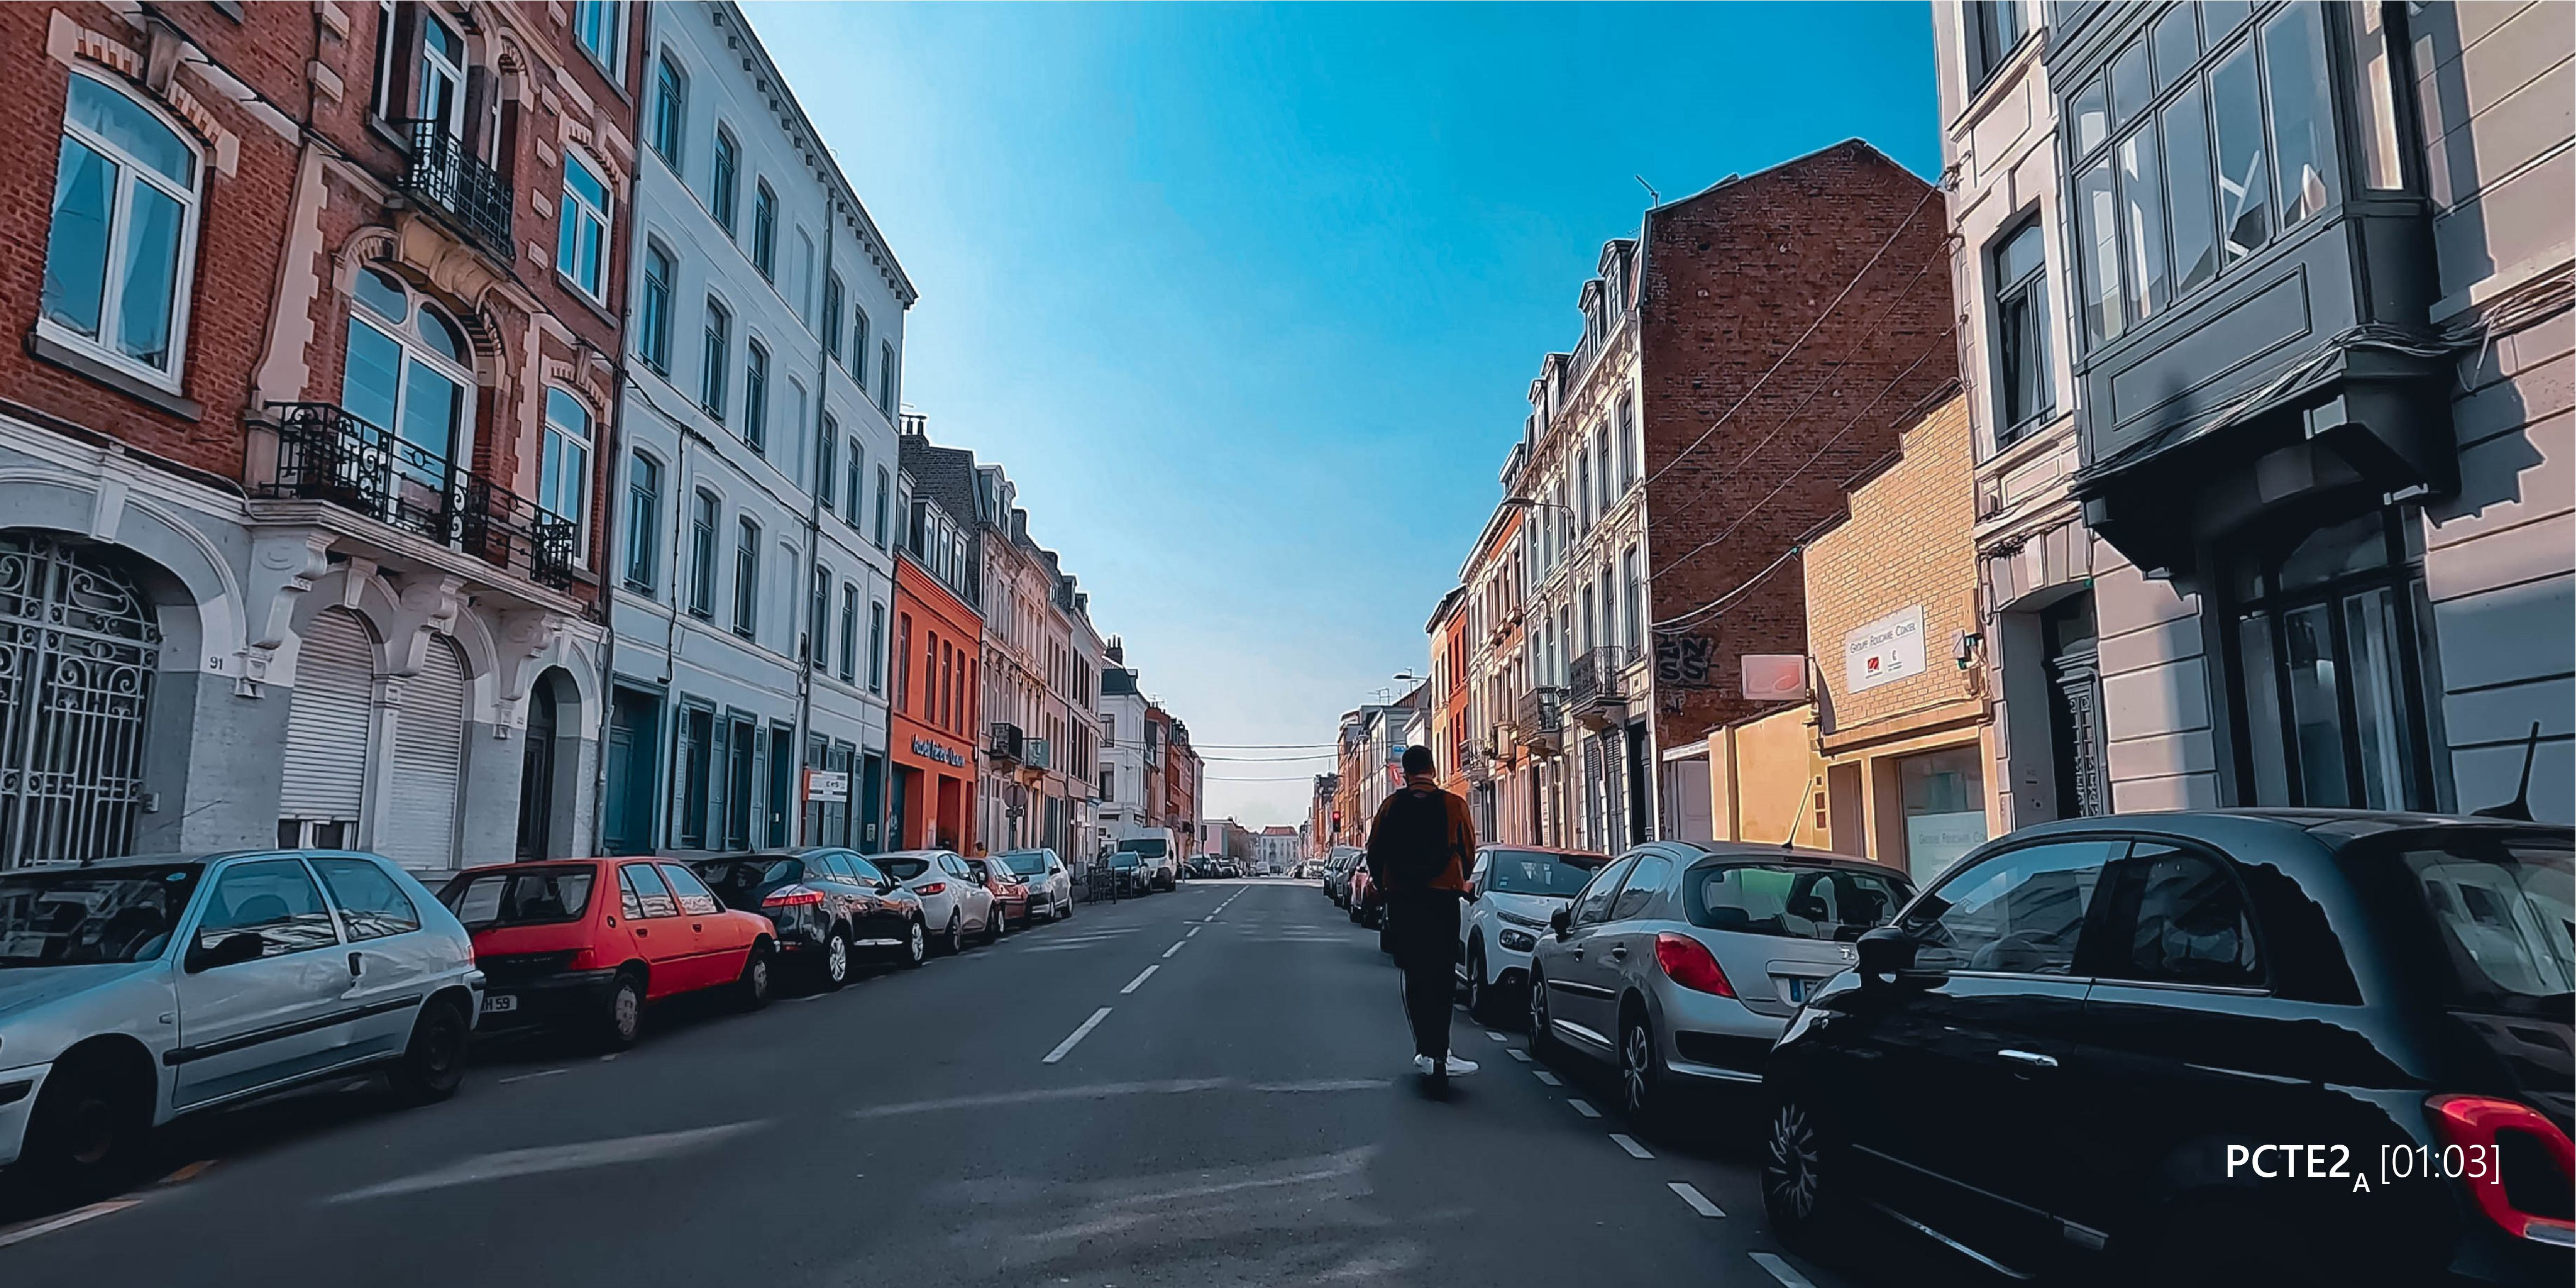
\includegraphics[width=0.75\columnwidth]{src/Figures/Annexes/Extrait_Video_PCTE2_Access_1.jpg}}
        \vspace{5pt}
        \begin{flushright}\scriptsize{
        Author: \textcolor{blue}{Dylan Moinse (2022)}
        }\end{flushright}
    \end{figure}

    % PCTE2 Photo Access 2
    \begin{figure}[h!]\vspace*{4pt}
        \caption*{Excerpt No. 2 from the video during the access segment (\(PCTE^{A}_{2}\))}
        \centerline{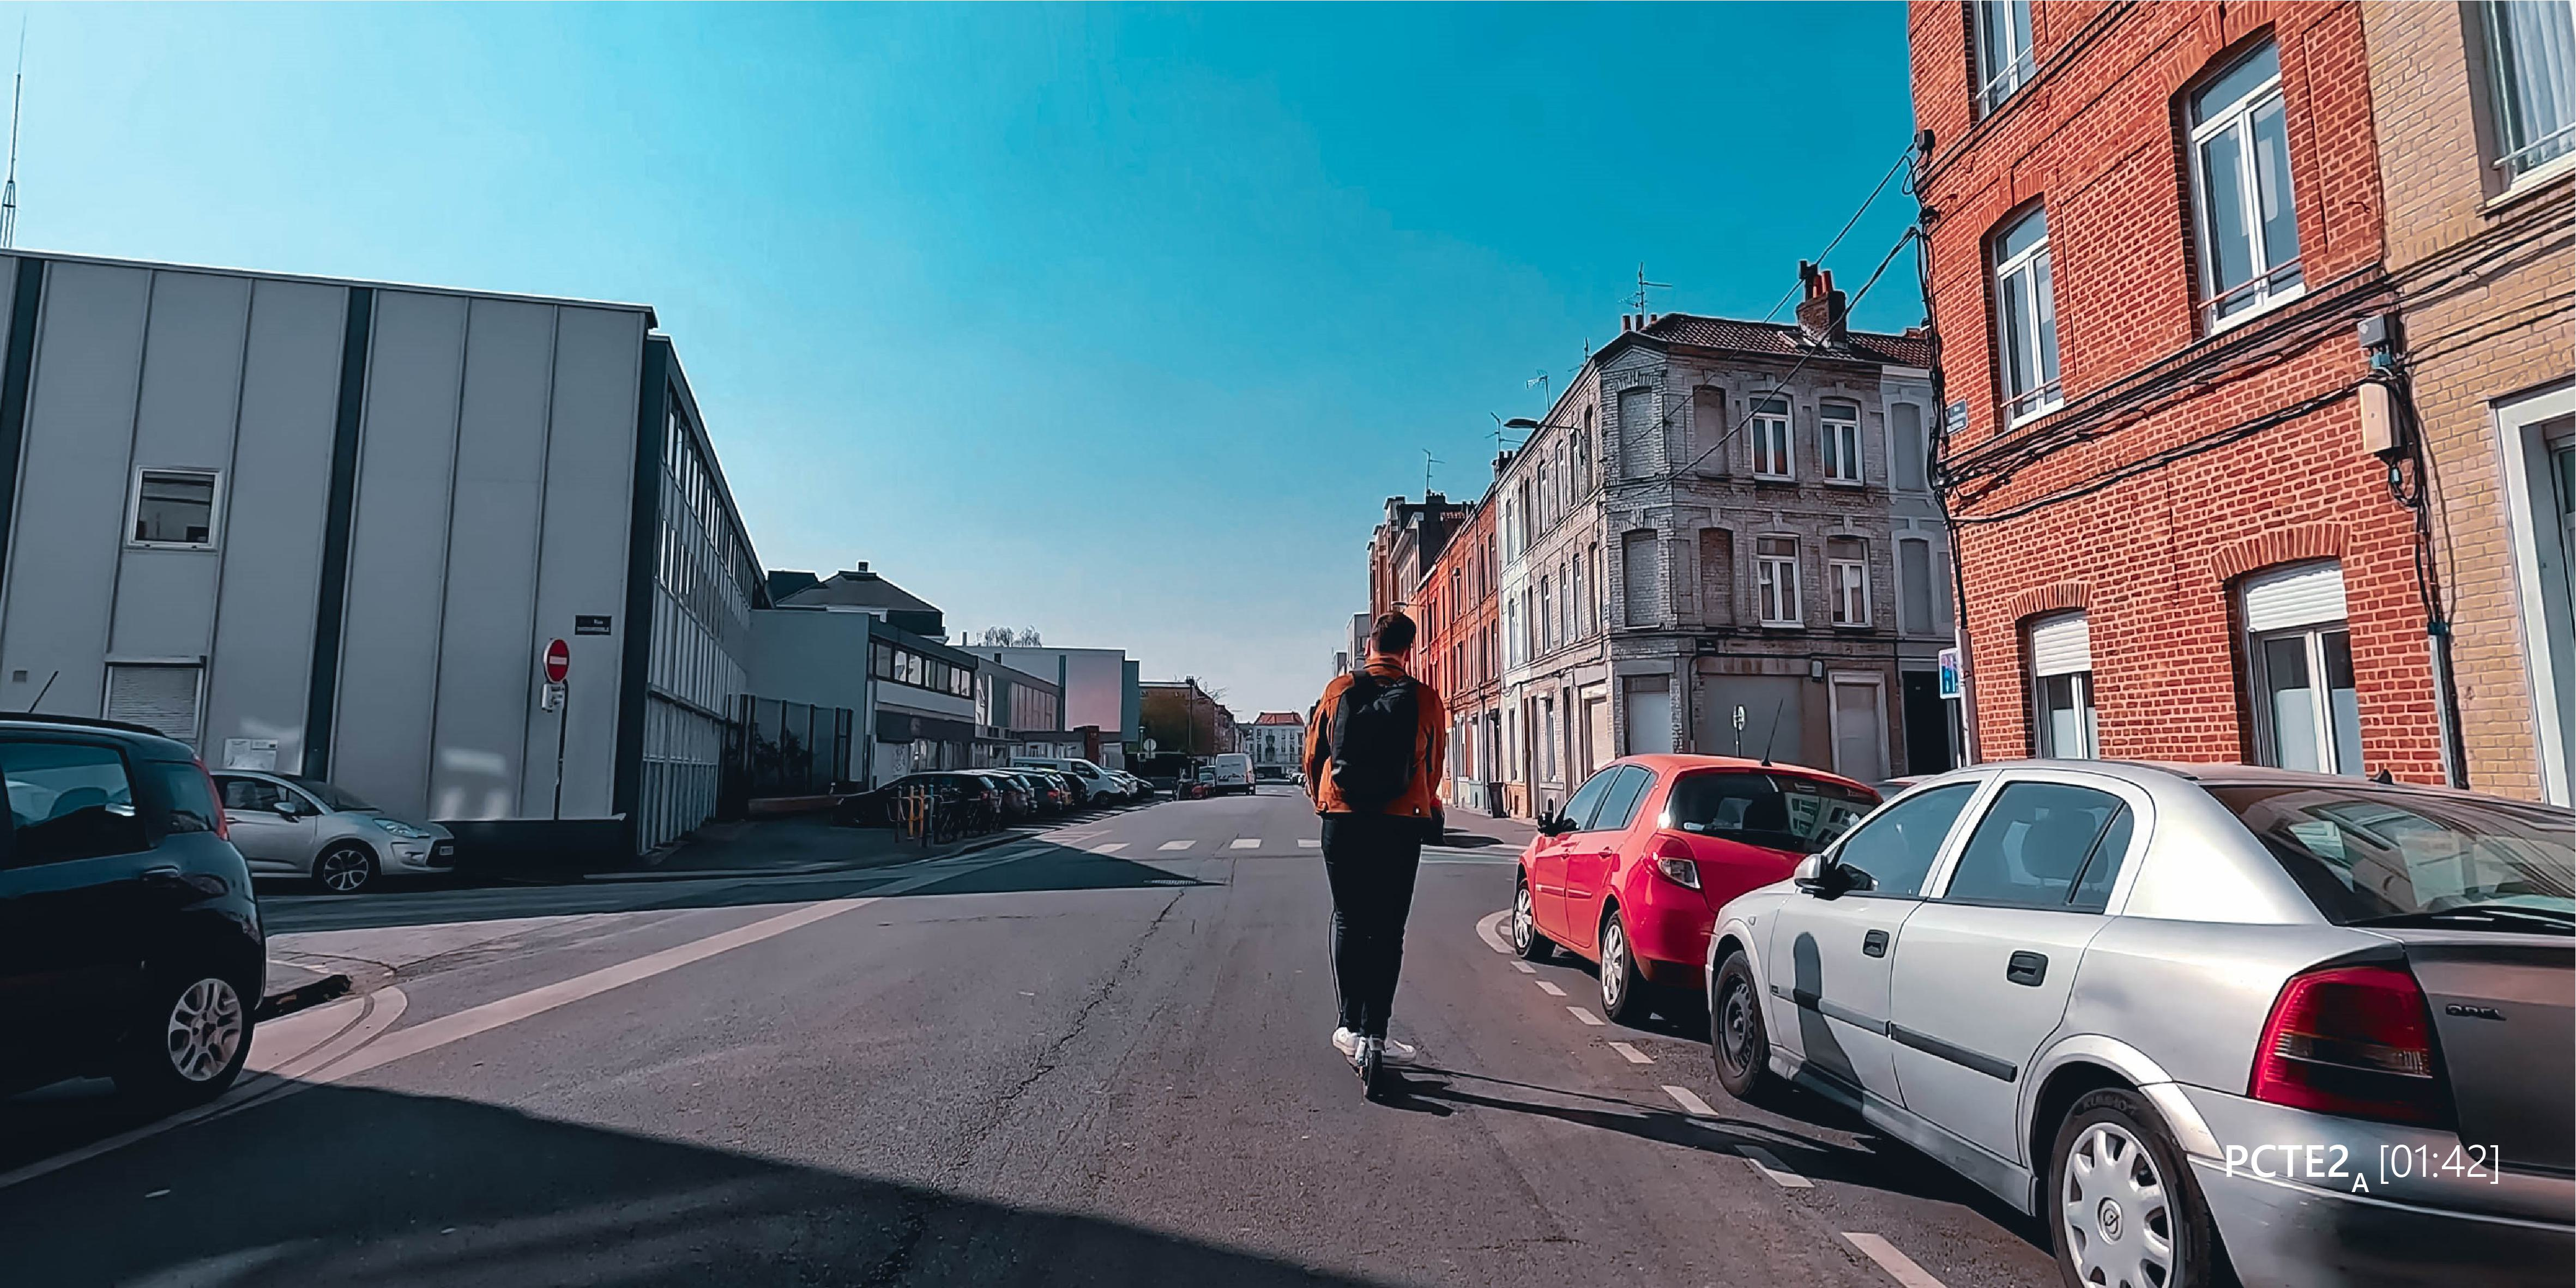
\includegraphics[width=0.75\columnwidth]{src/Figures/Annexes/Extrait_Video_PCTE2_Access_2.jpg}}
        \vspace{5pt}
        \begin{flushright}\scriptsize{
        Author: \textcolor{blue}{Dylan Moinse (2022)}
        }\end{flushright}
    \end{figure}
    
    % PCTE2 Photo Access 3
    \begin{figure}[h!]\vspace*{4pt}
        \caption*{Excerpt No. 3 from the video during the access segment (\(PCTE^{A}_{2}\))}
        \centerline{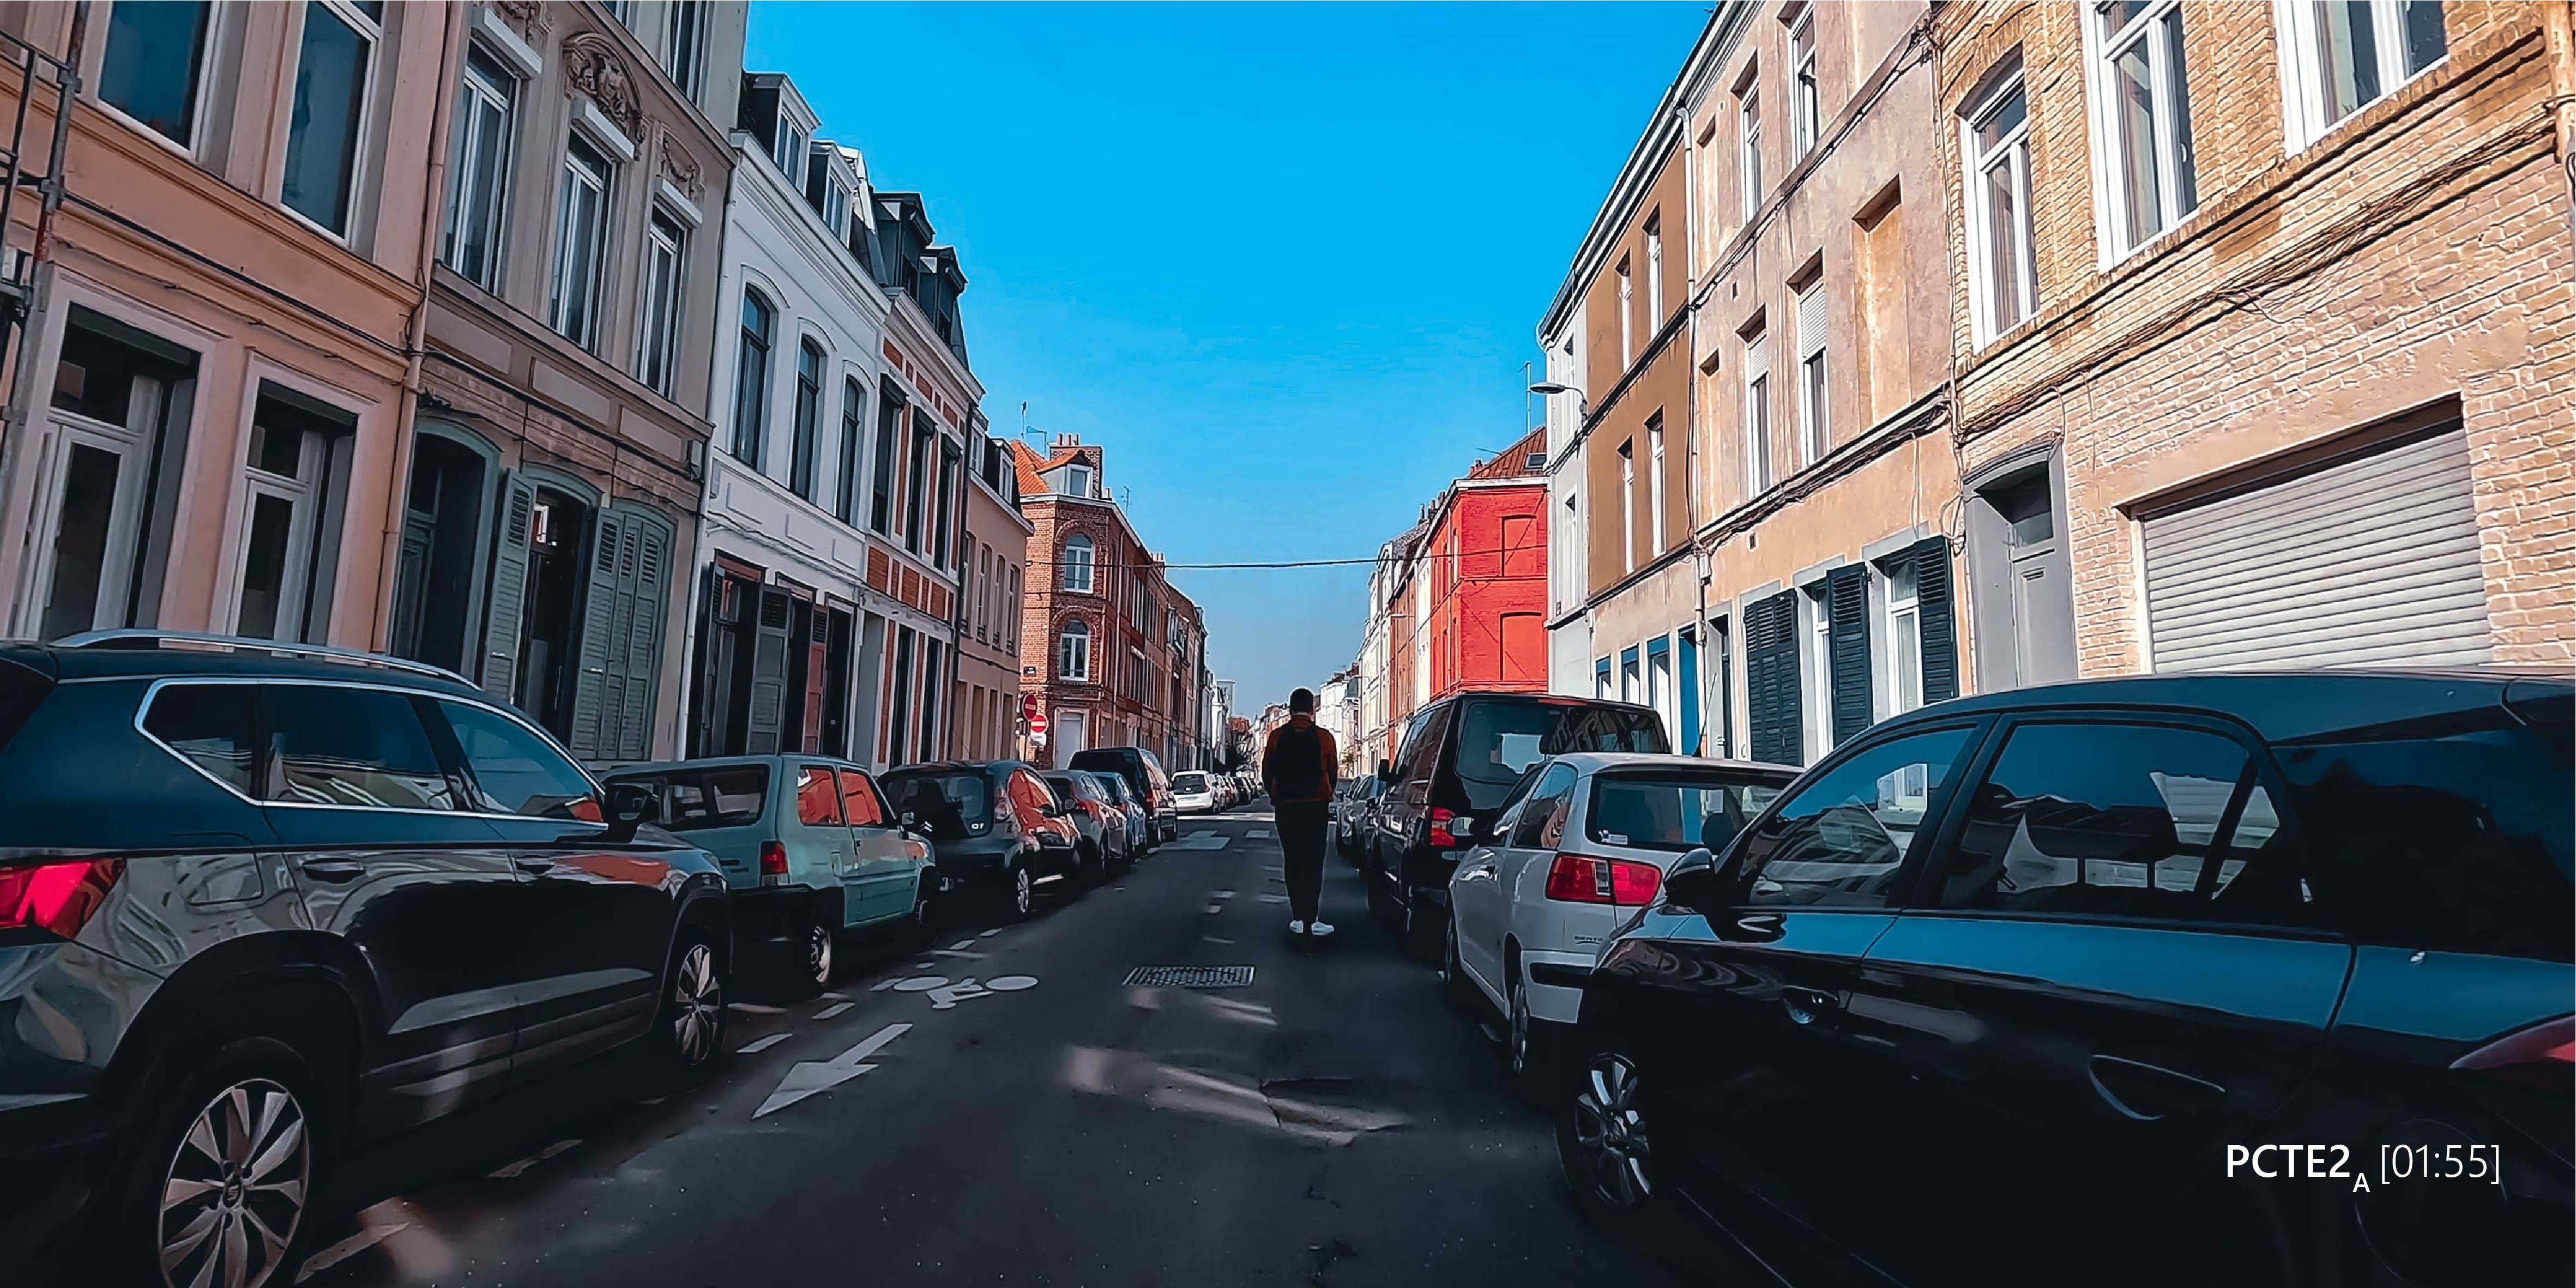
\includegraphics[width=0.75\columnwidth]{src/Figures/Annexes/Extrait_Video_PCTE2_Access_3.jpg}}
        \vspace{5pt}
        \begin{flushright}\scriptsize{
        Author: \textcolor{blue}{Dylan Moinse (2022)}
        }\end{flushright}
    \end{figure}

    % PCTE2 Photo Access 4
    \begin{figure}[h!]\vspace*{4pt}
        \caption*{Excerpt No. 4 from the video during the access segment (\(PCTE^{A}_{2}\))}
        \centerline{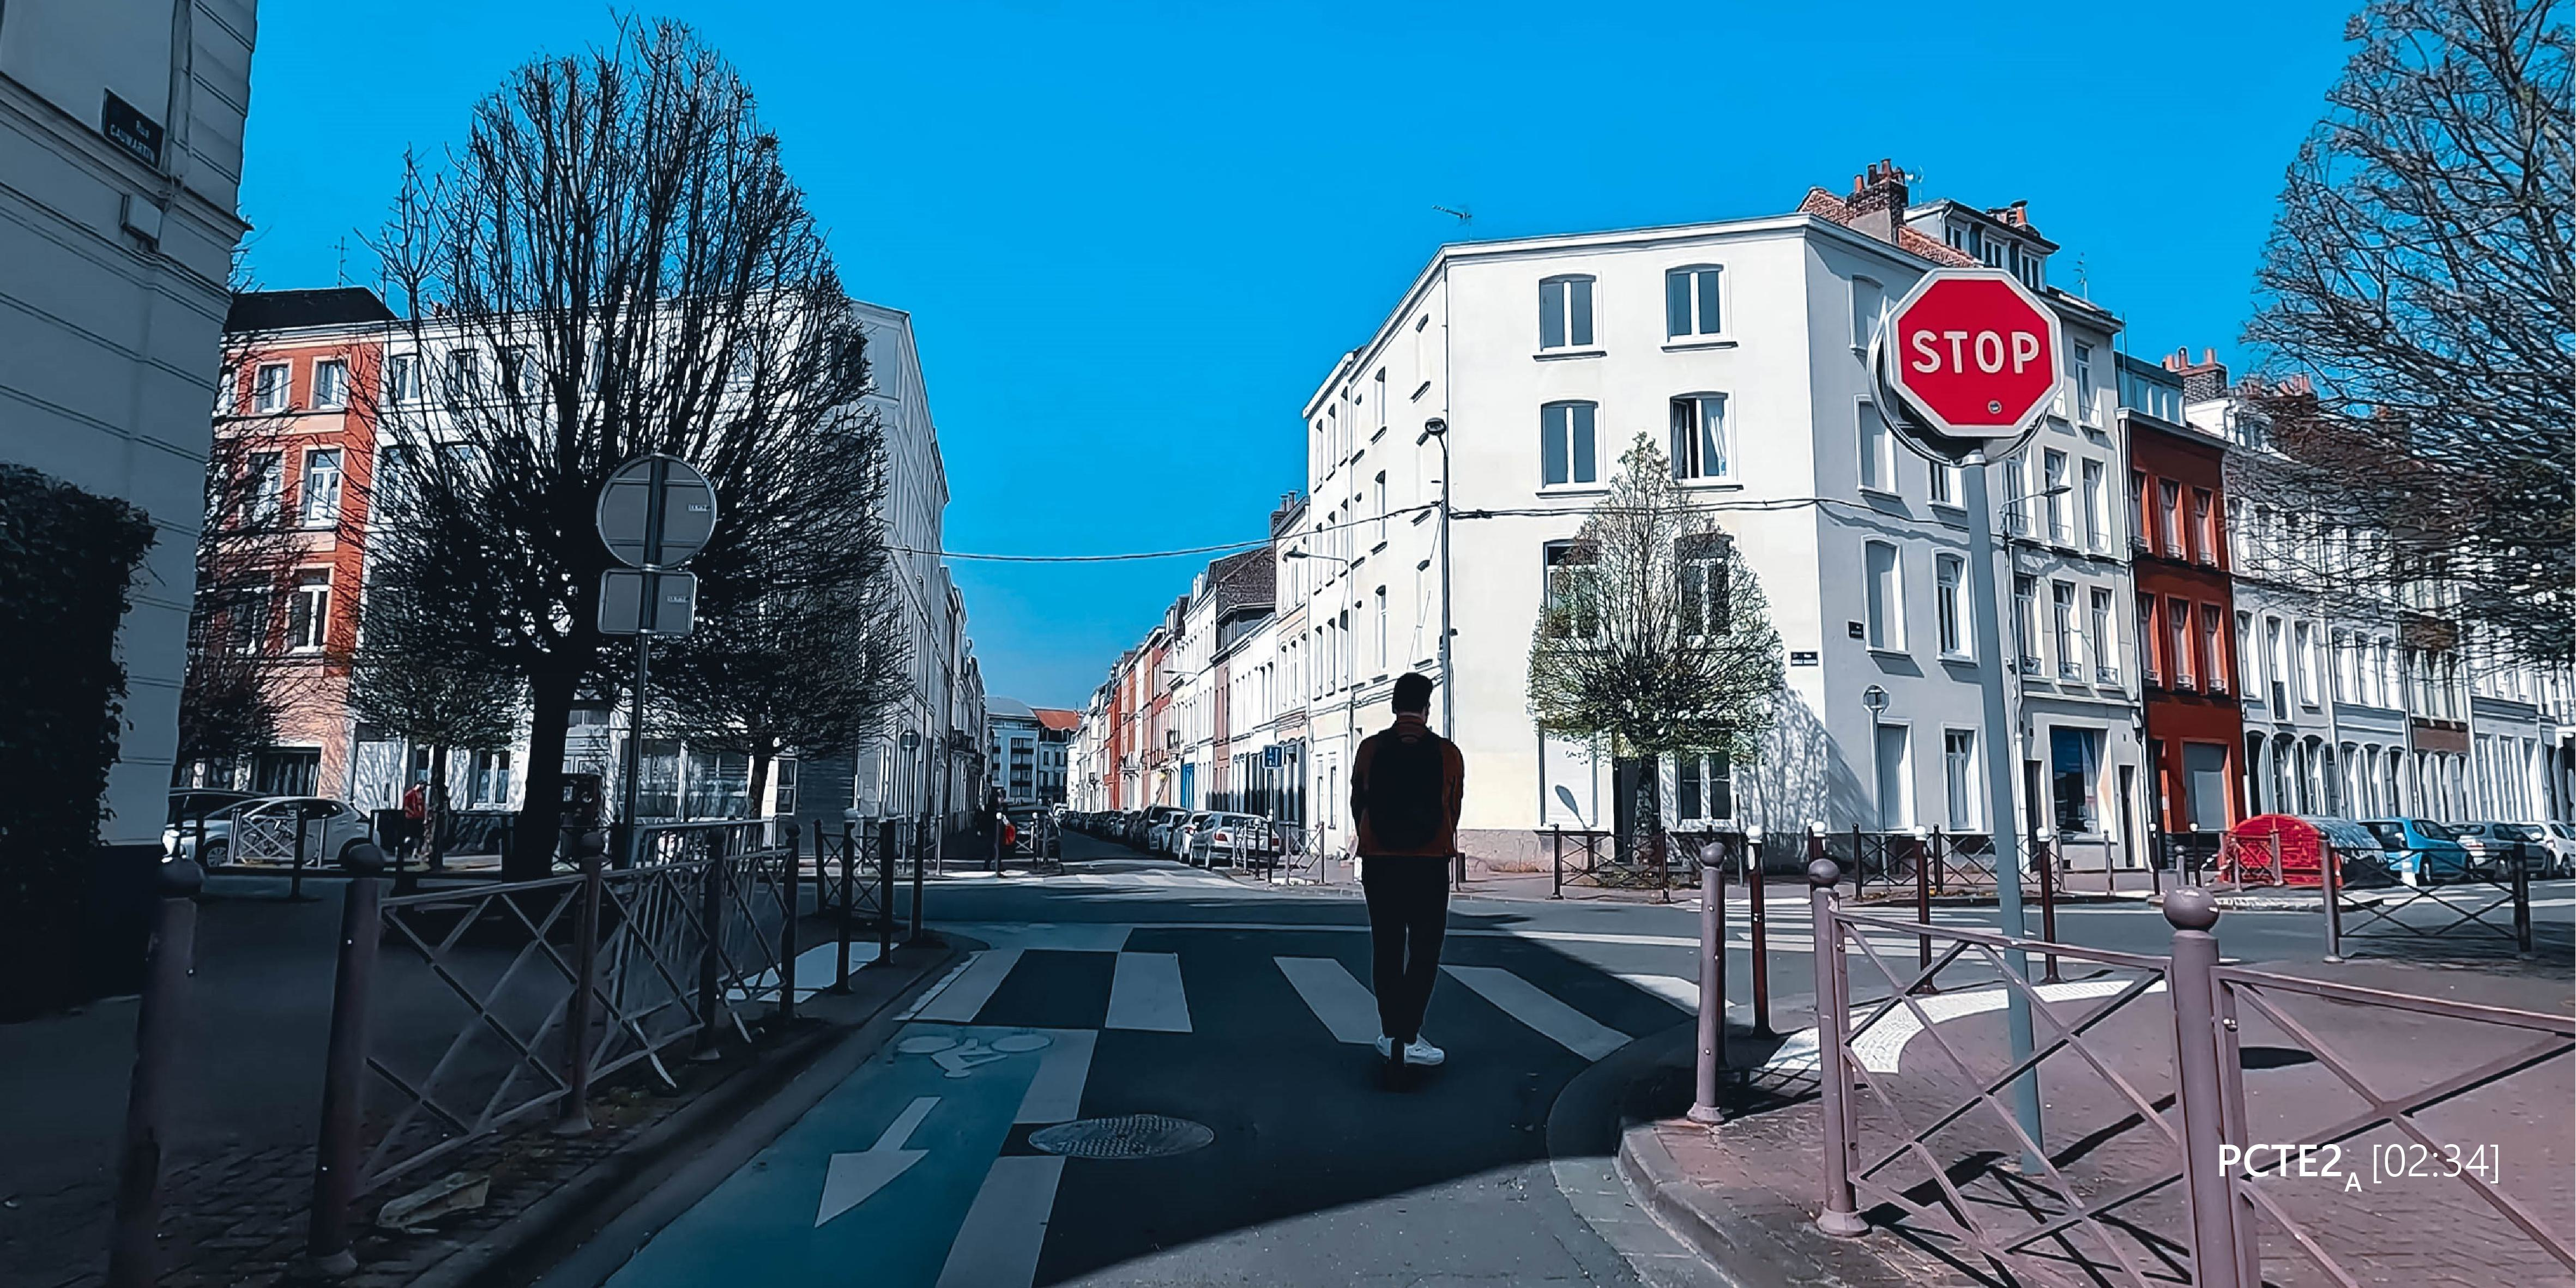
\includegraphics[width=0.75\columnwidth]{src/Figures/Annexes/Extrait_Video_PCTE2_Access_4.jpg}}
        \vspace{5pt}
        \begin{flushright}\scriptsize{
        Author: \textcolor{blue}{Dylan Moinse (2022)}
        }\end{flushright}
    \end{figure}

    % PCTE2 Photo Access 5
    \begin{figure}[h!]\vspace*{4pt}
        \caption*{Excerpt No. 5 from the video during the access segment (\(PCTE^{A}_{2}\))}
        \centerline{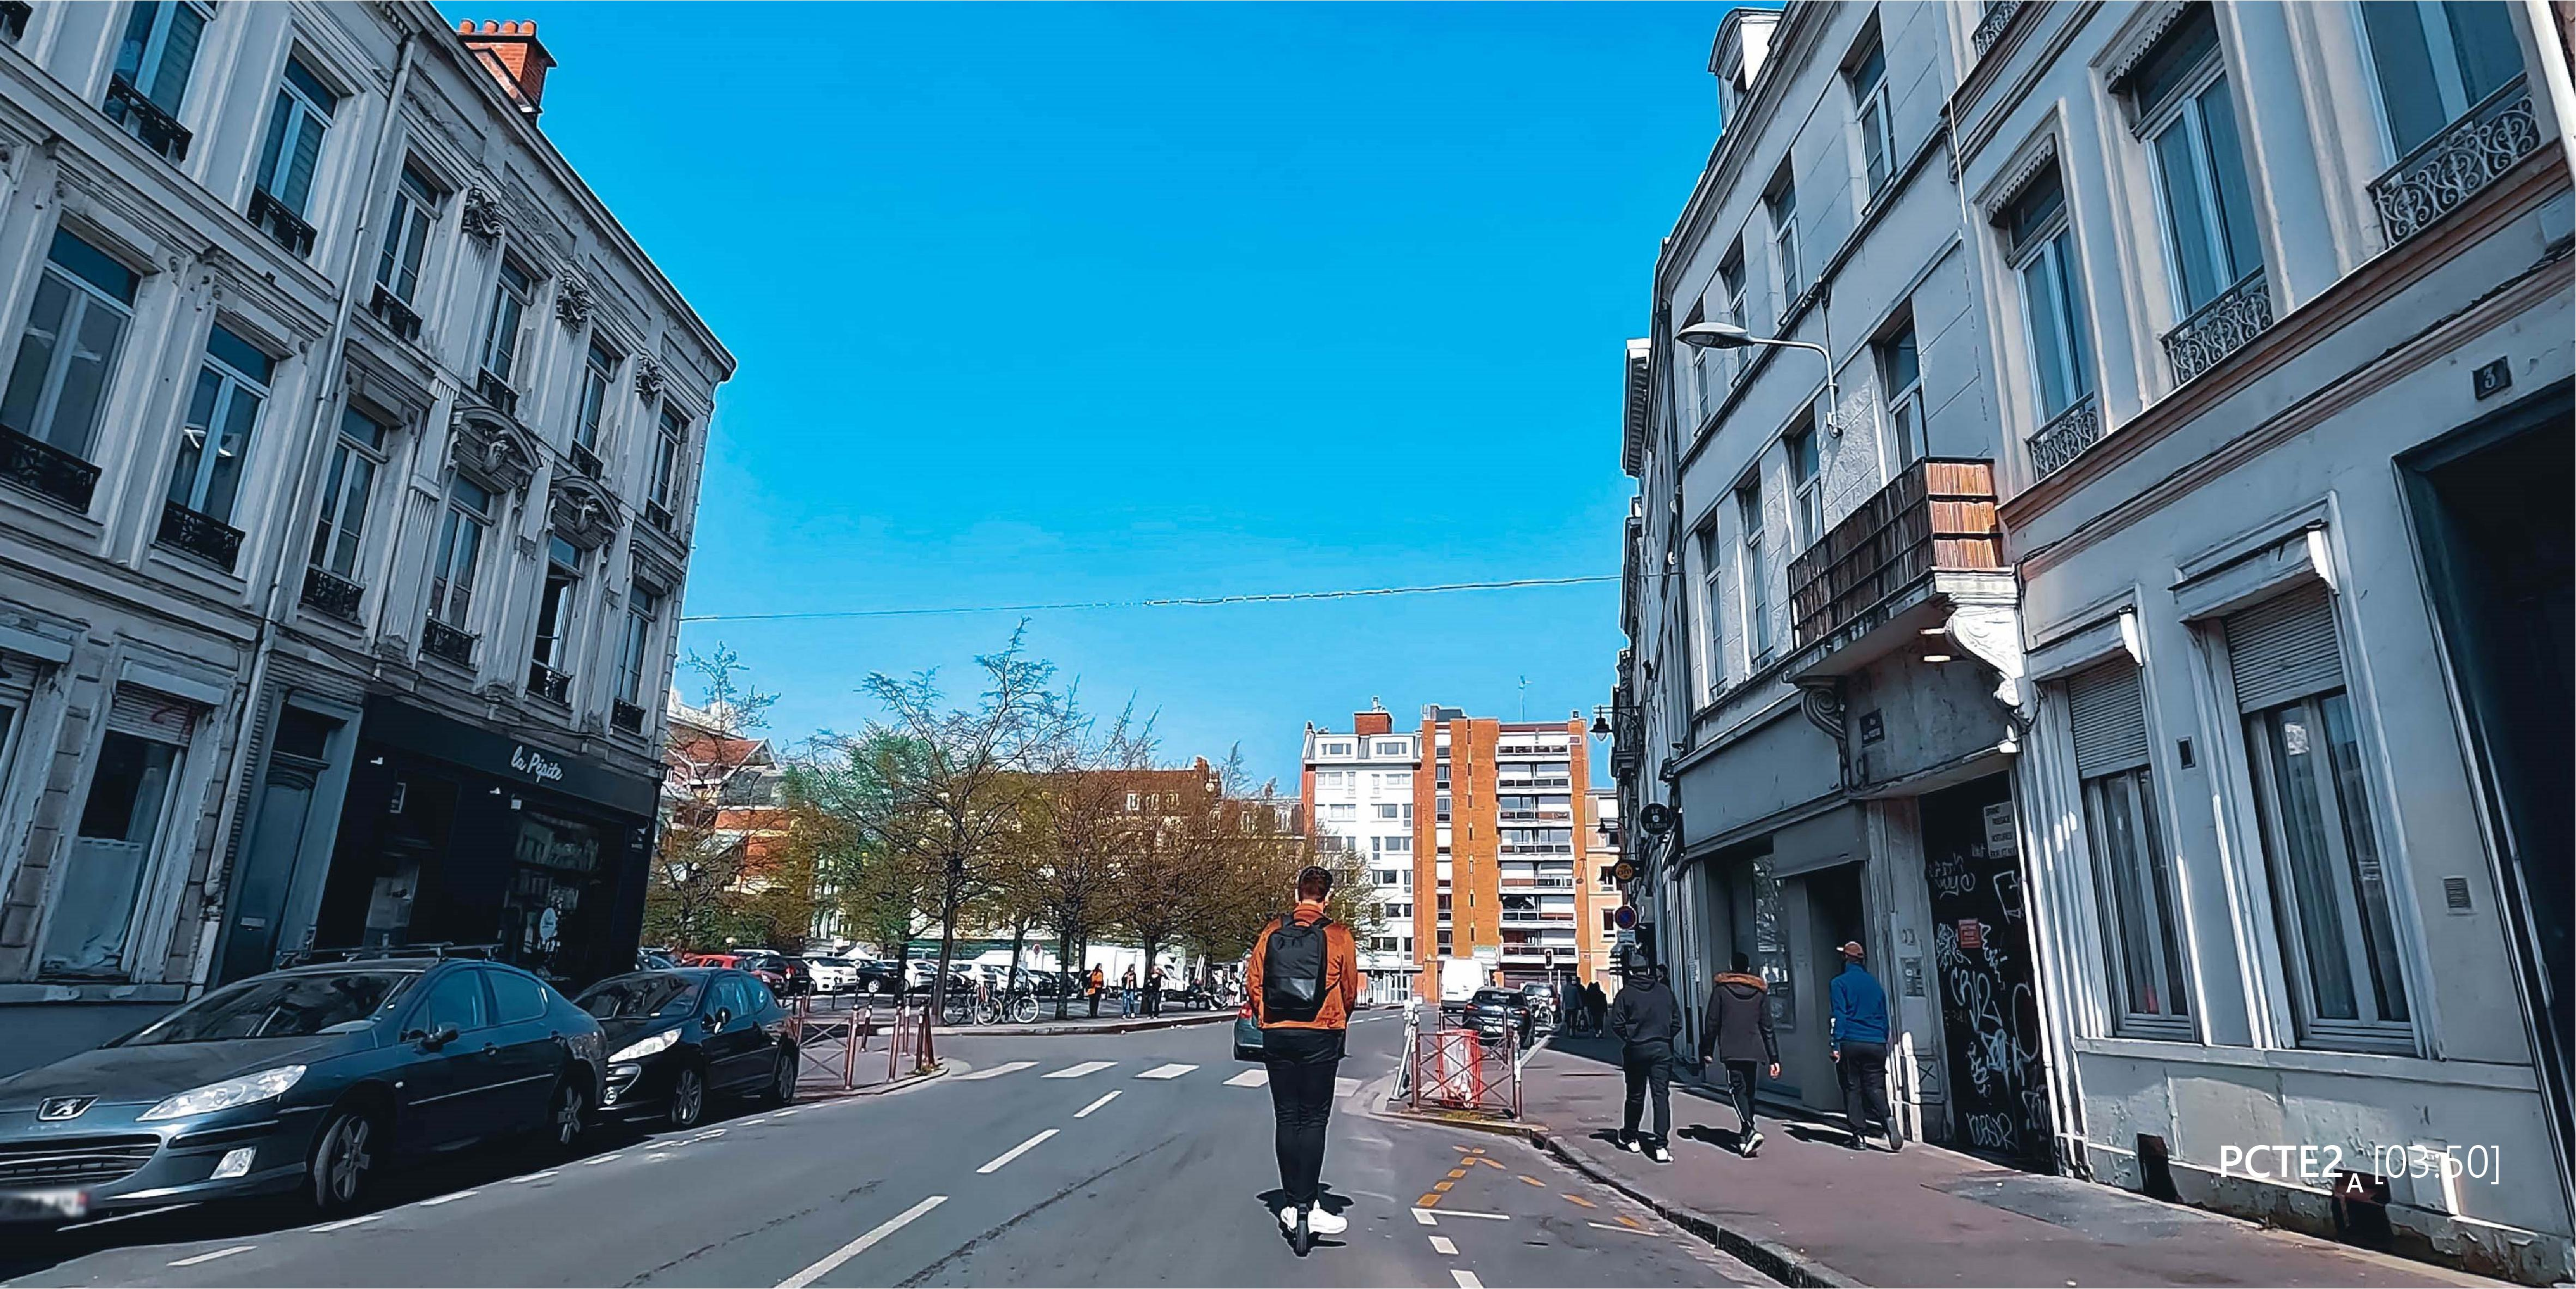
\includegraphics[width=0.75\columnwidth]{src/Figures/Annexes/Extrait_Video_PCTE2_Access_5.jpg}}
        \vspace{5pt}
        \begin{flushright}\scriptsize{
        Author: \textcolor{blue}{Dylan Moinse (2022)}
        }\end{flushright}
    \end{figure}

    % PCTE2 Photo Access 6
    \begin{figure}[h!]\vspace*{4pt}
        \caption*{Excerpt No. 6 from the video during the access segment (\(PCTE^{A}_{2}\))}
        \centerline{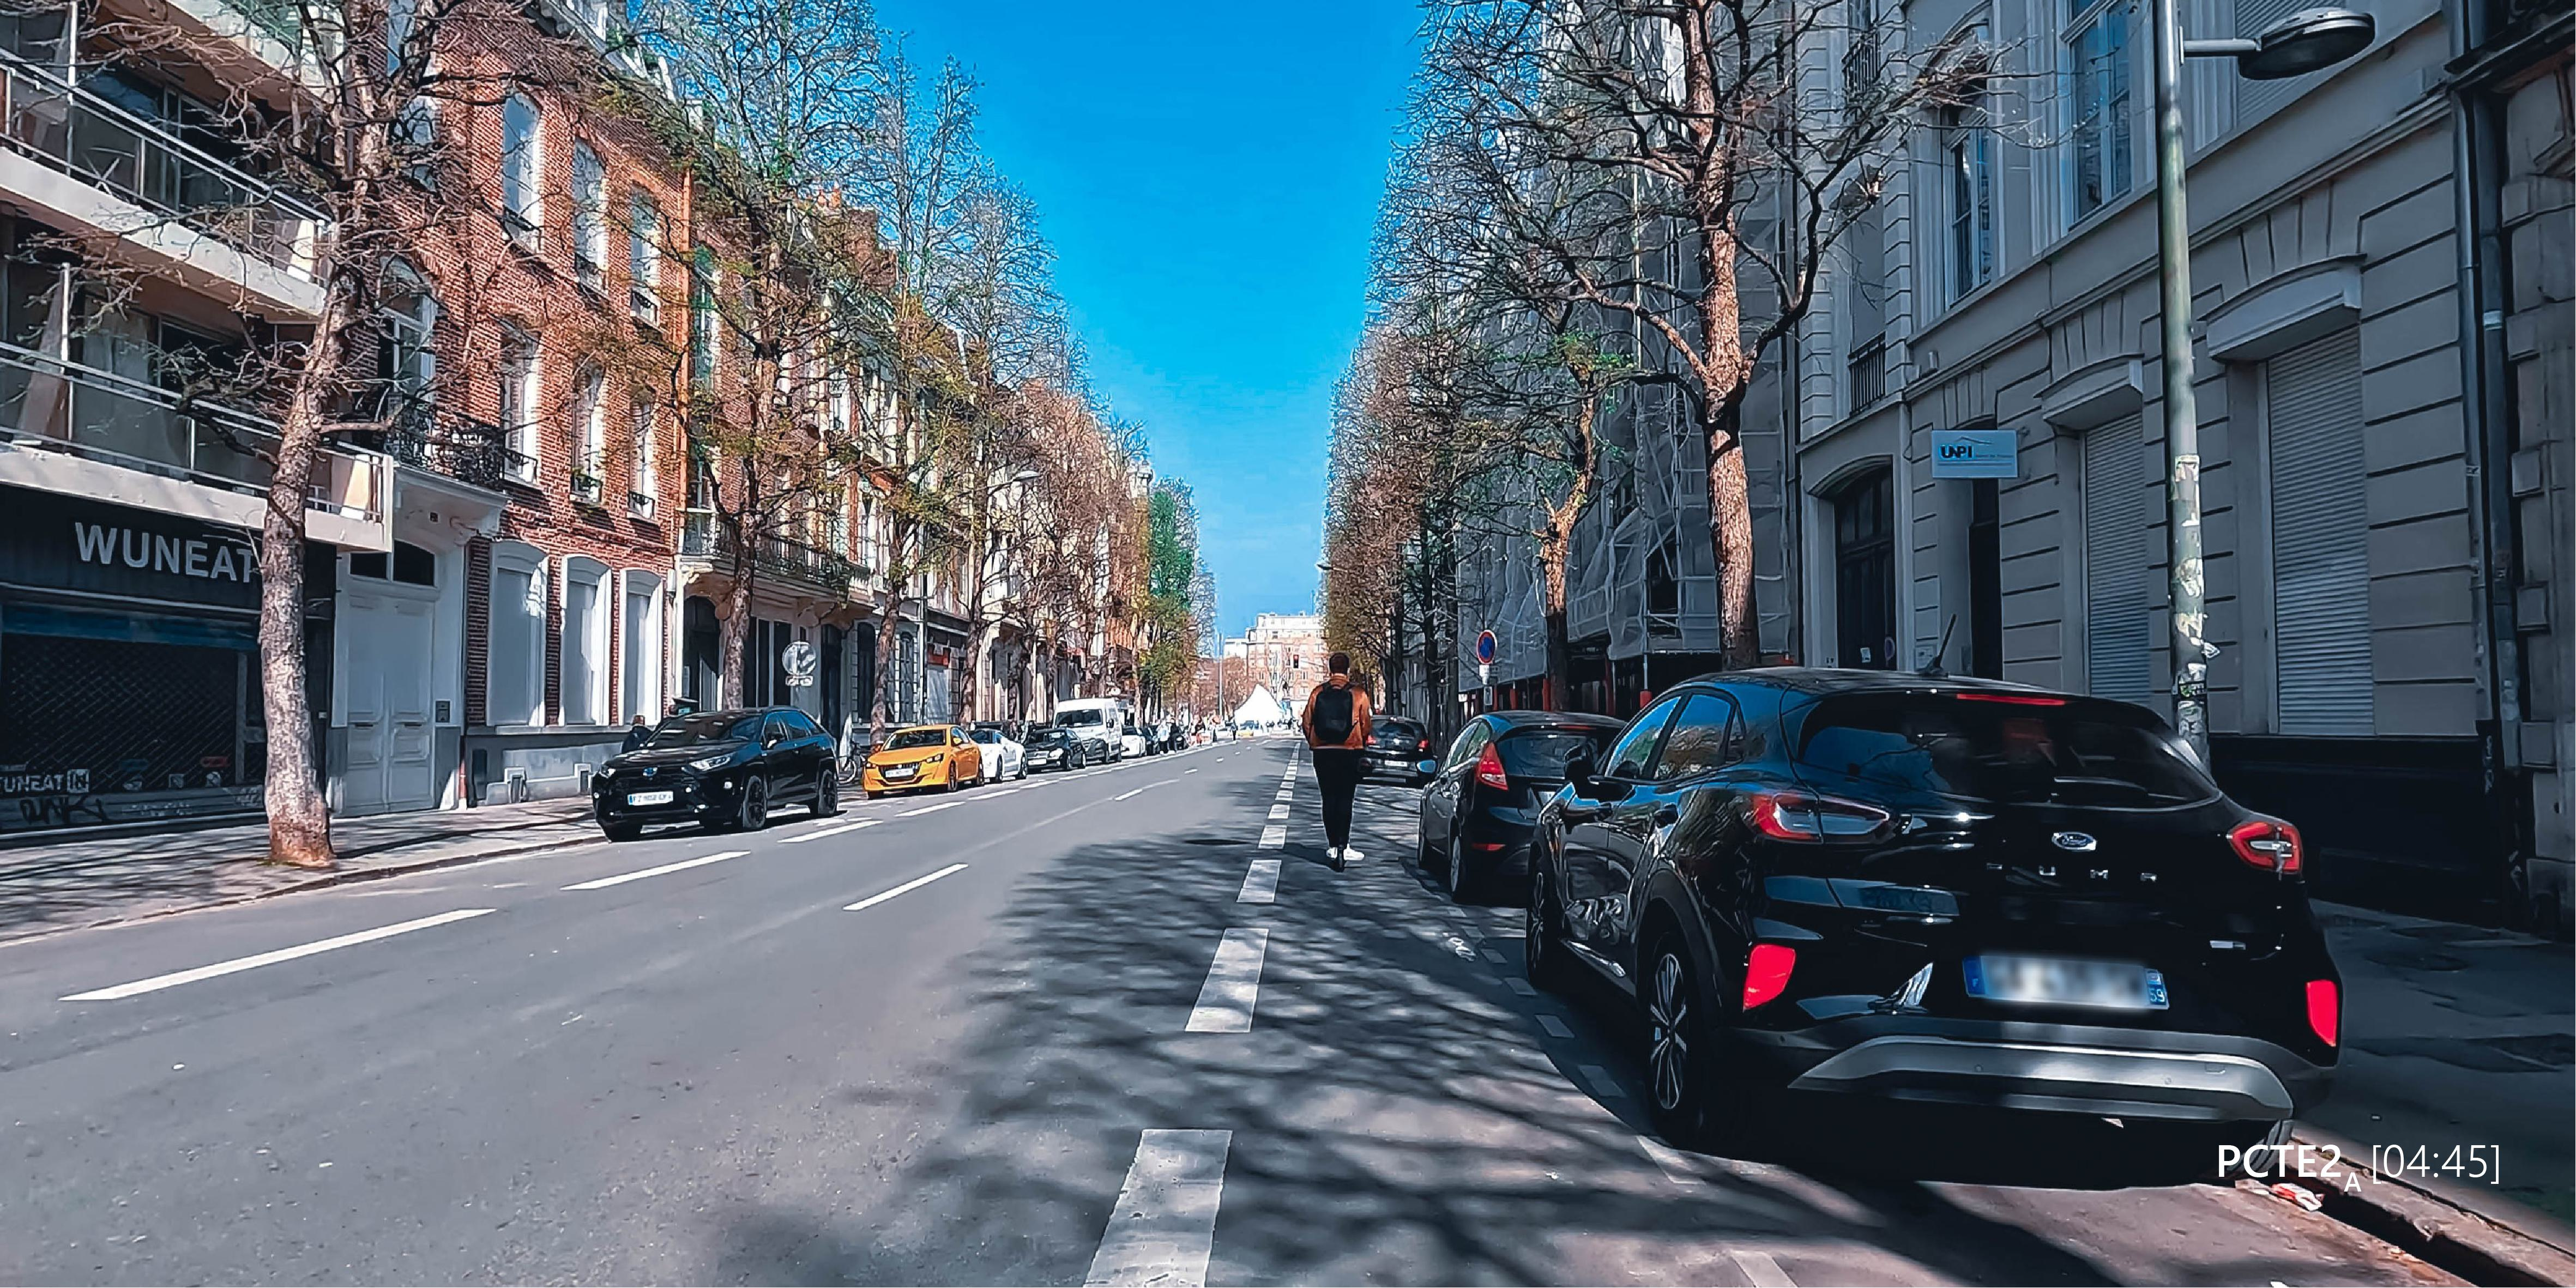
\includegraphics[width=0.75\columnwidth]{src/Figures/Annexes/Extrait_Video_PCTE2_Access_6.jpg}}
        \vspace{5pt}
        \begin{flushright}\scriptsize{
        Author: \textcolor{blue}{Dylan Moinse (2022)}
        }\end{flushright}
    \end{figure}

    % PCTE2 Photo Access 7
    \begin{figure}[h!]\vspace*{4pt}
        \caption*{Excerpt No. 7 from the video during the access segment (\(PCTE^{A}_{2}\))}
        \centerline{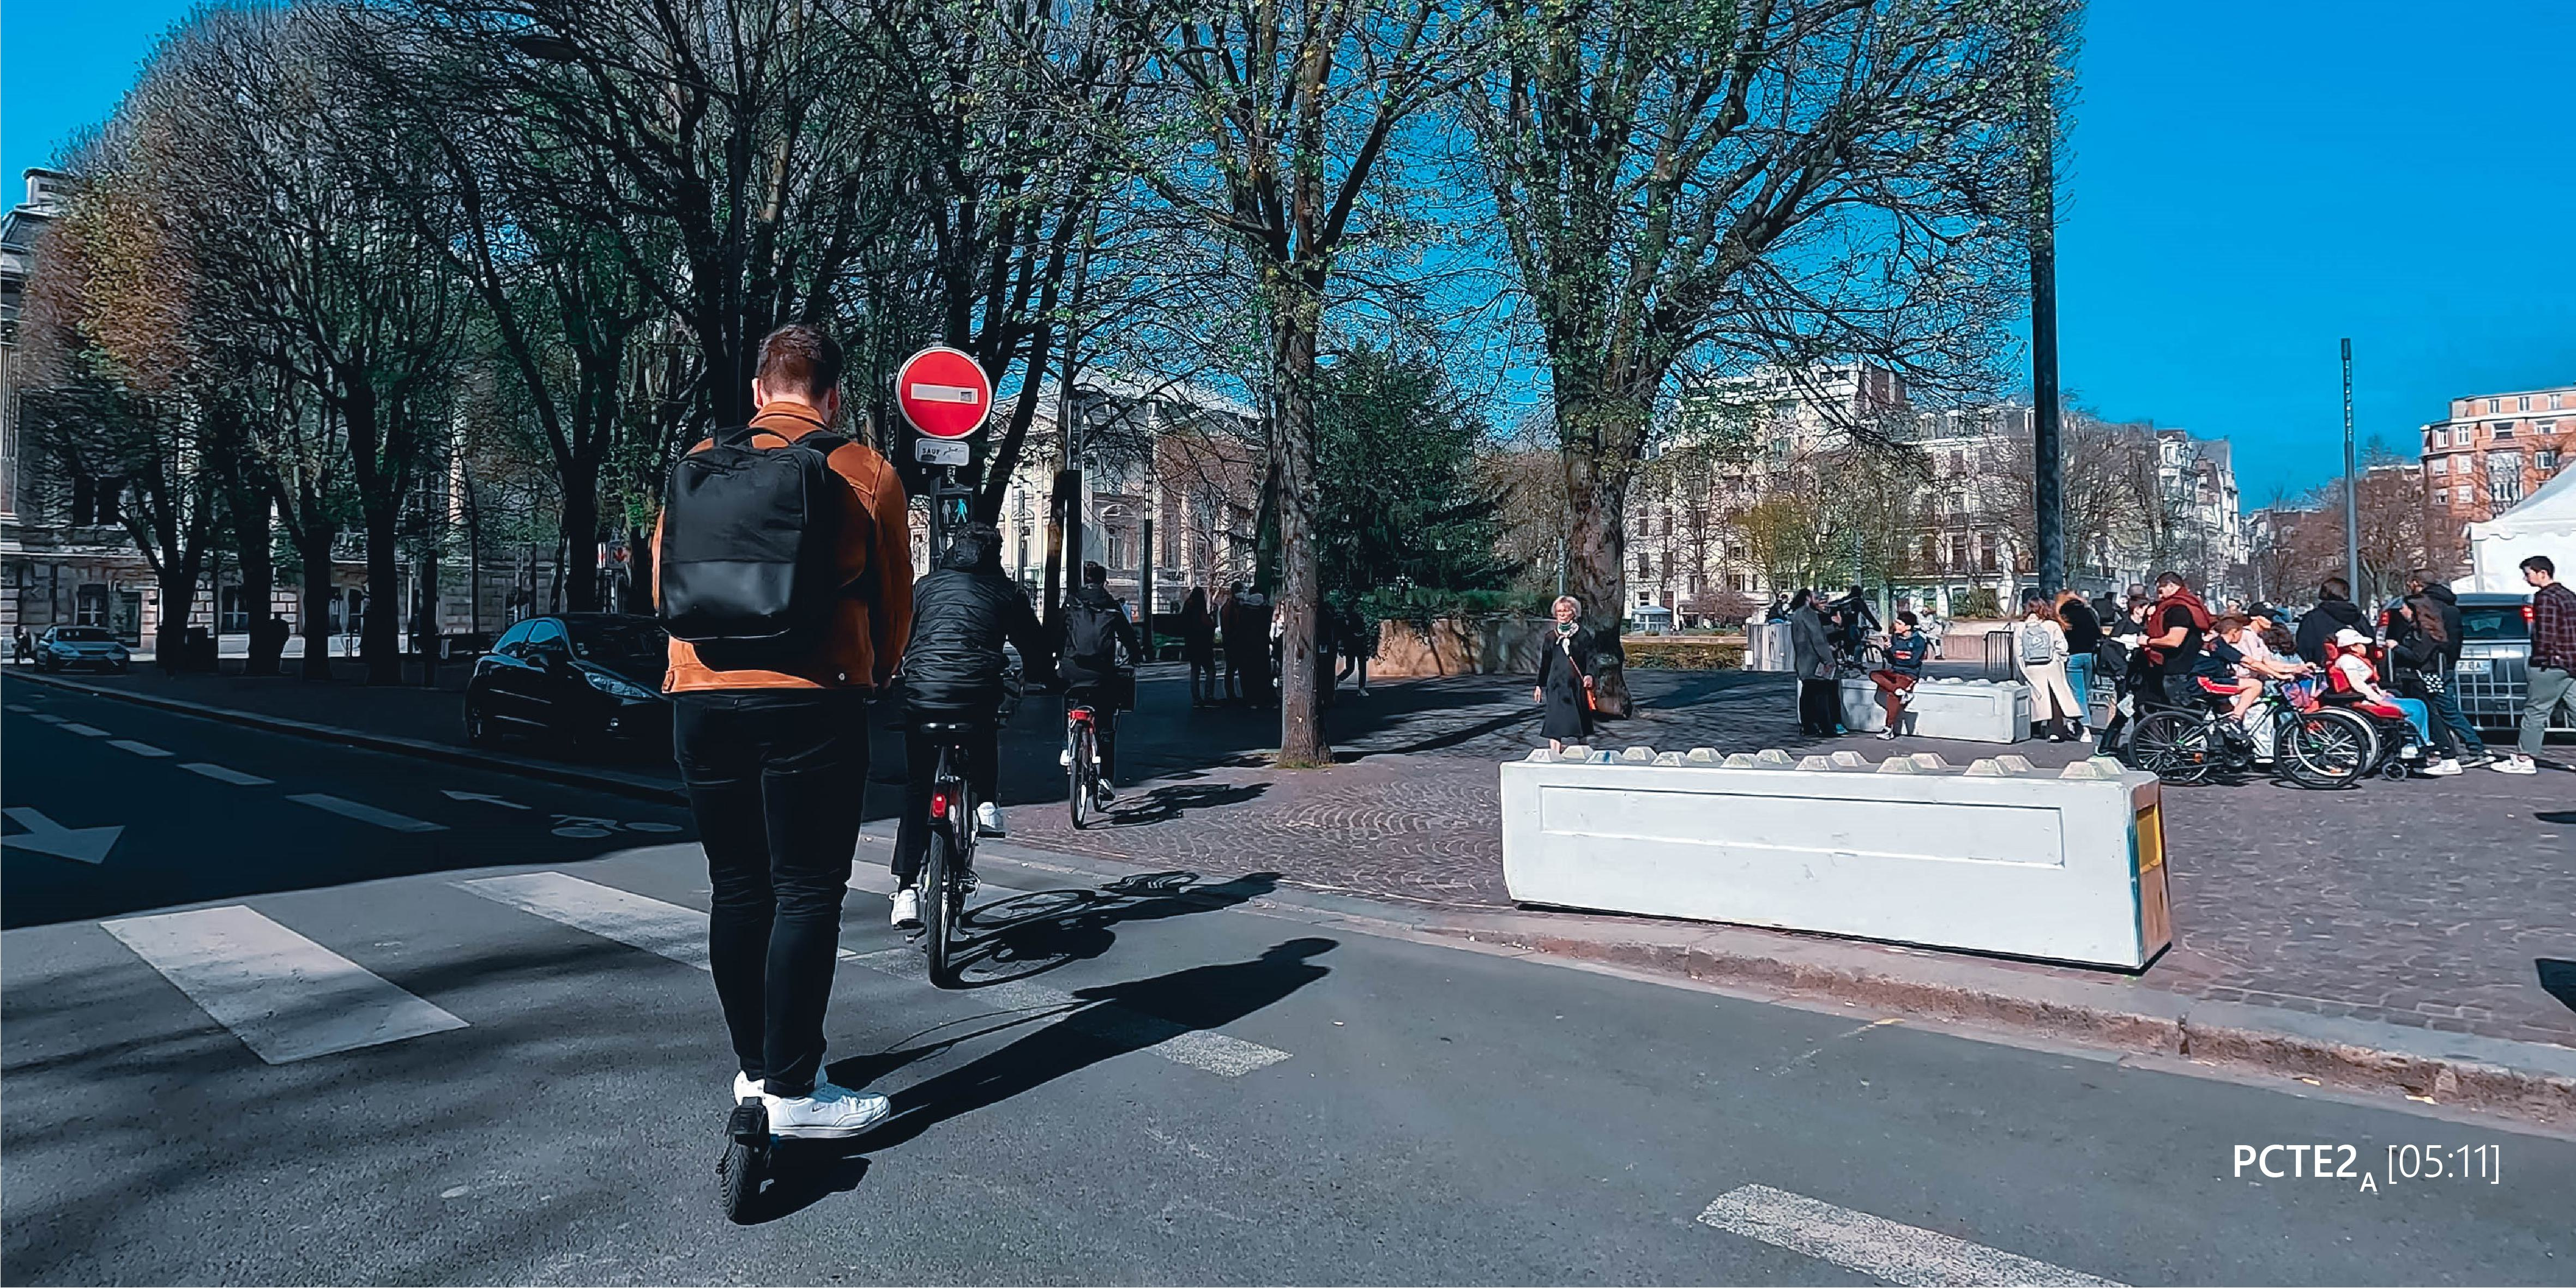
\includegraphics[width=0.75\columnwidth]{src/Figures/Annexes/Extrait_Video_PCTE2_Access_7.jpg}}
        \vspace{5pt}
        \begin{flushright}\scriptsize{
        Author: \textcolor{blue}{Dylan Moinse (2022)}
        }\end{flushright}
    \end{figure}

    % Photos PCTE2 TC
\subsubsection{Selection of Images Extracted During the Metro Trip}

    % PCTE2 Photo TC 1
    \begin{figure}[h!]\vspace*{4pt}
        \caption*{Excerpt No. 1 from the video during the metro trip (\(PCTE^{TC}_{2}\))}
        \centerline{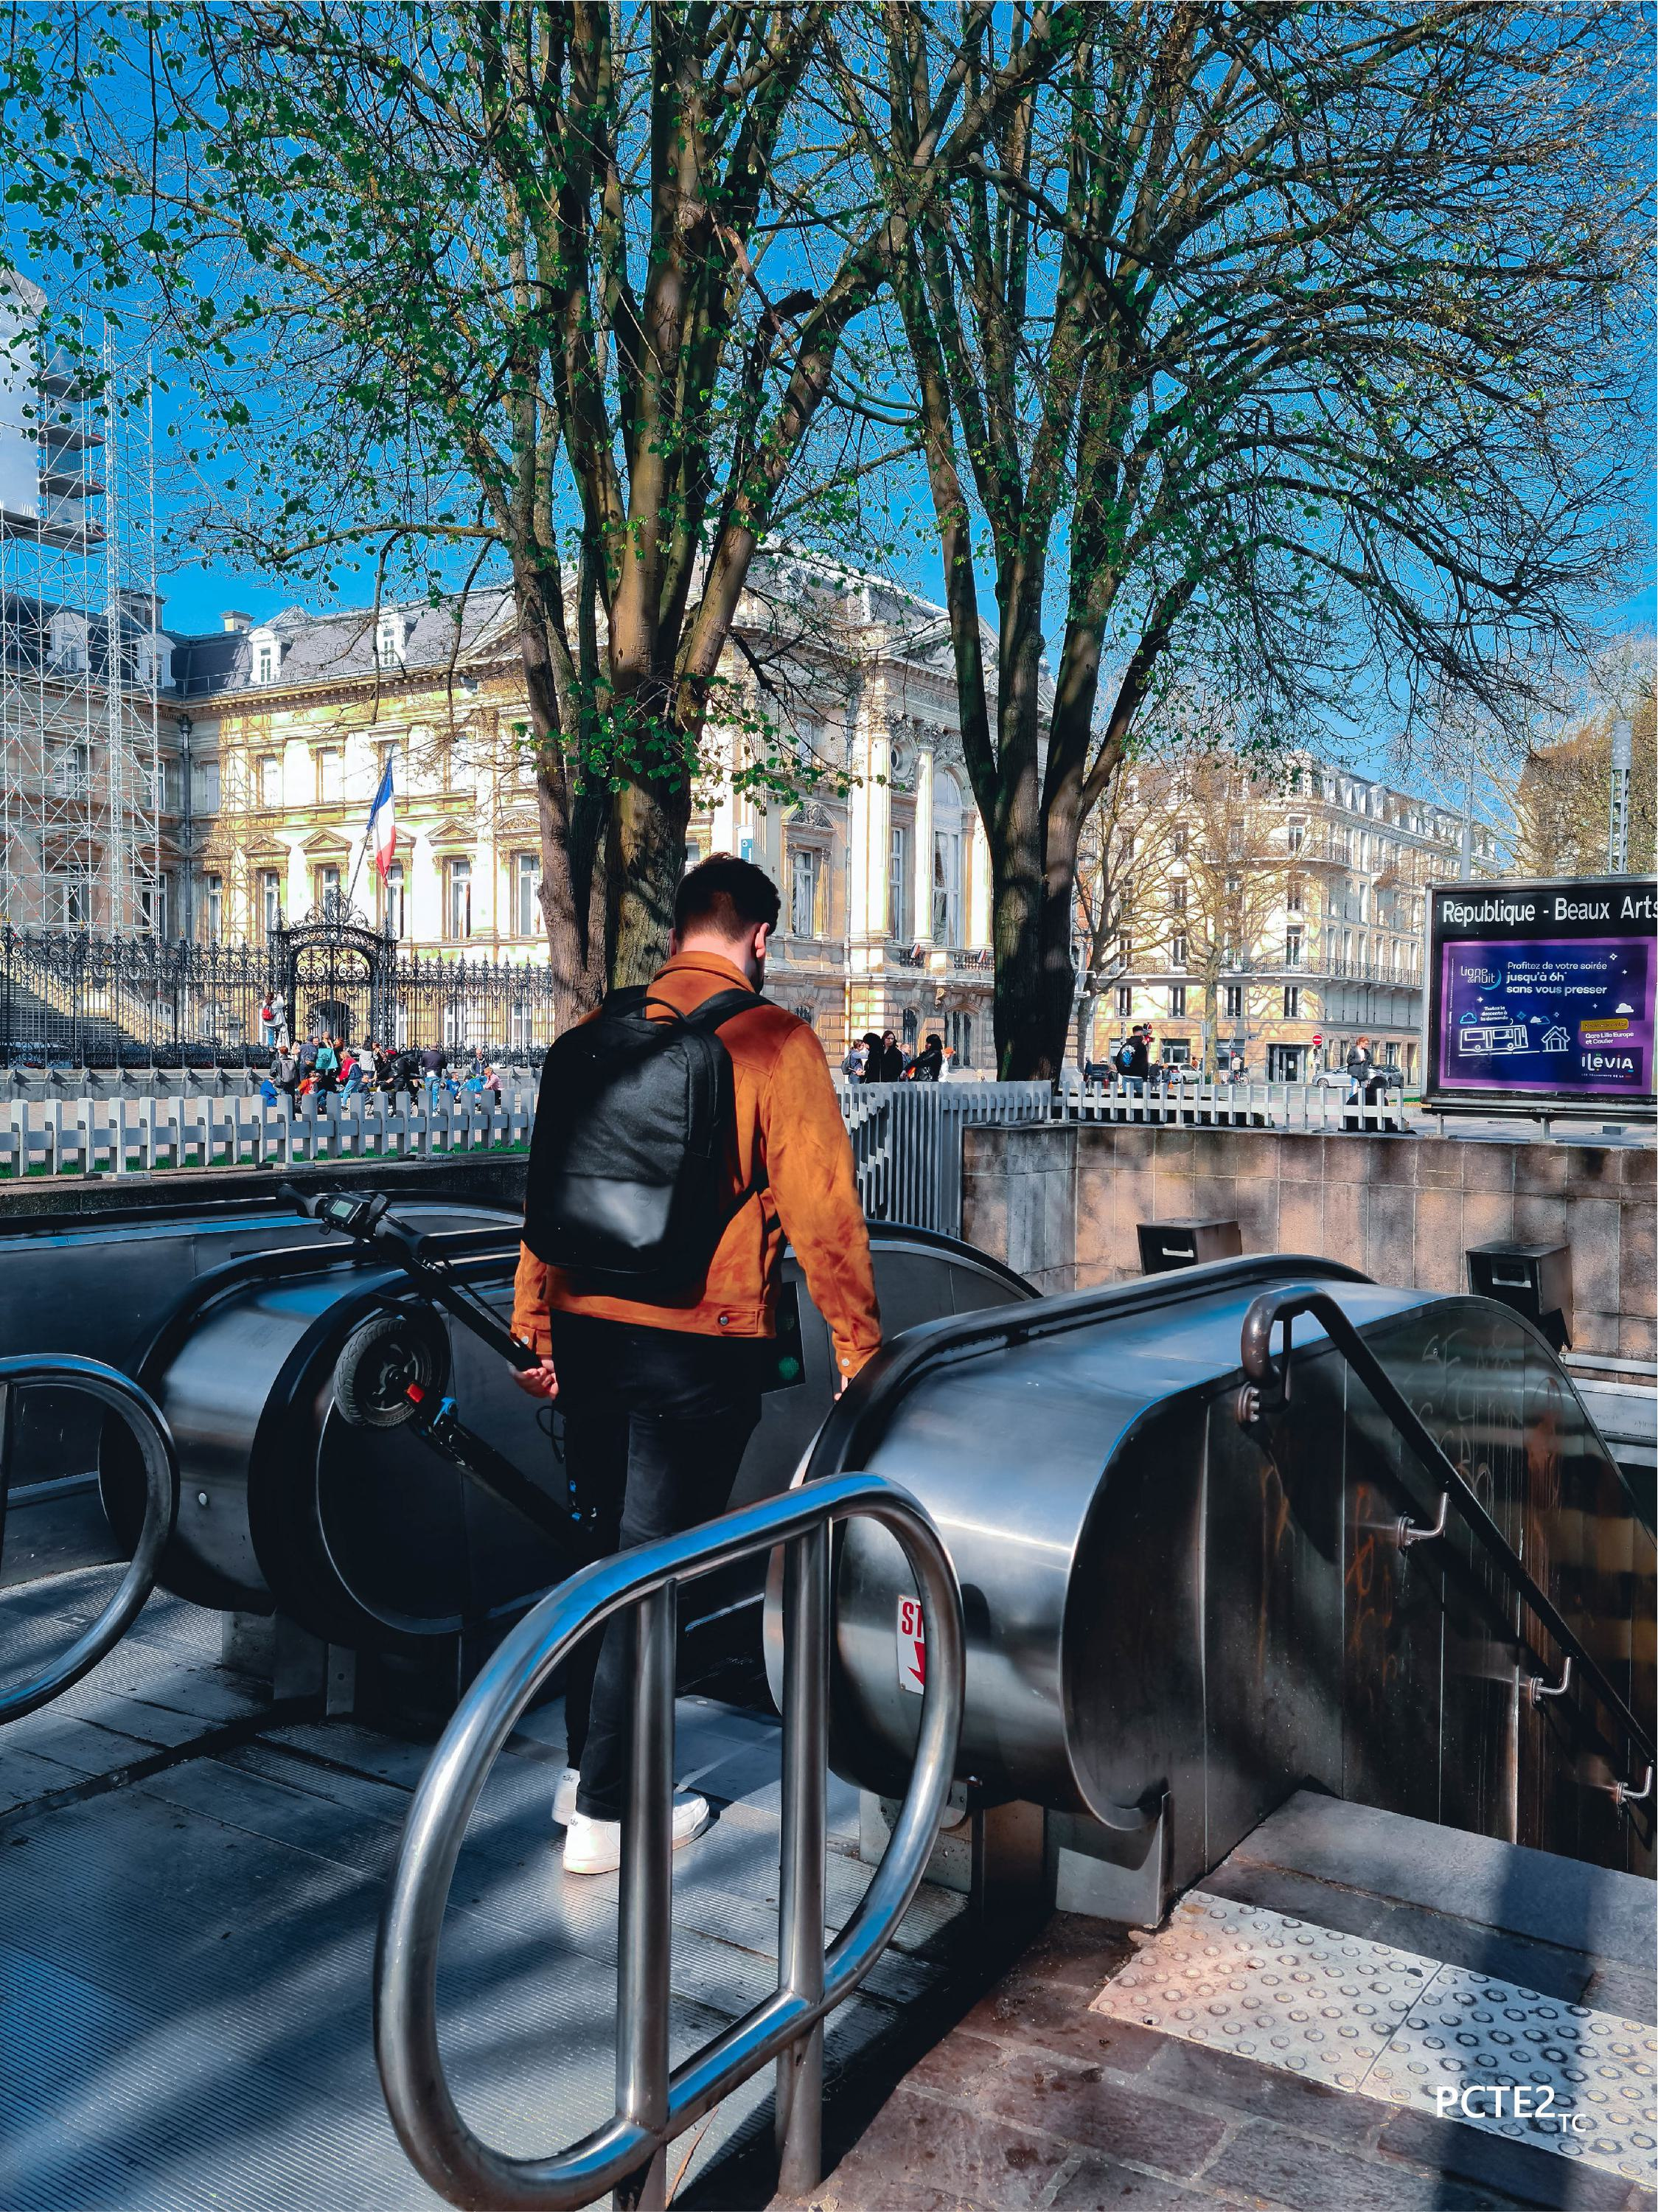
\includegraphics[width=0.5\columnwidth]{src/Figures/Annexes/Extrait_Video_PCTE2_TC_1.jpg}}
        \vspace{5pt}
        \begin{flushright}\scriptsize{
        Author: \textcolor{blue}{Dylan Moinse (2022)}
        }\end{flushright}
    \end{figure}

    % PCTE2 Photo TC 2
    \begin{figure}[h!]\vspace*{4pt}
        \caption*{Excerpt No. 2 from the video during the metro trip (\(PCTE^{TC}_{2}\))}
        \centerline{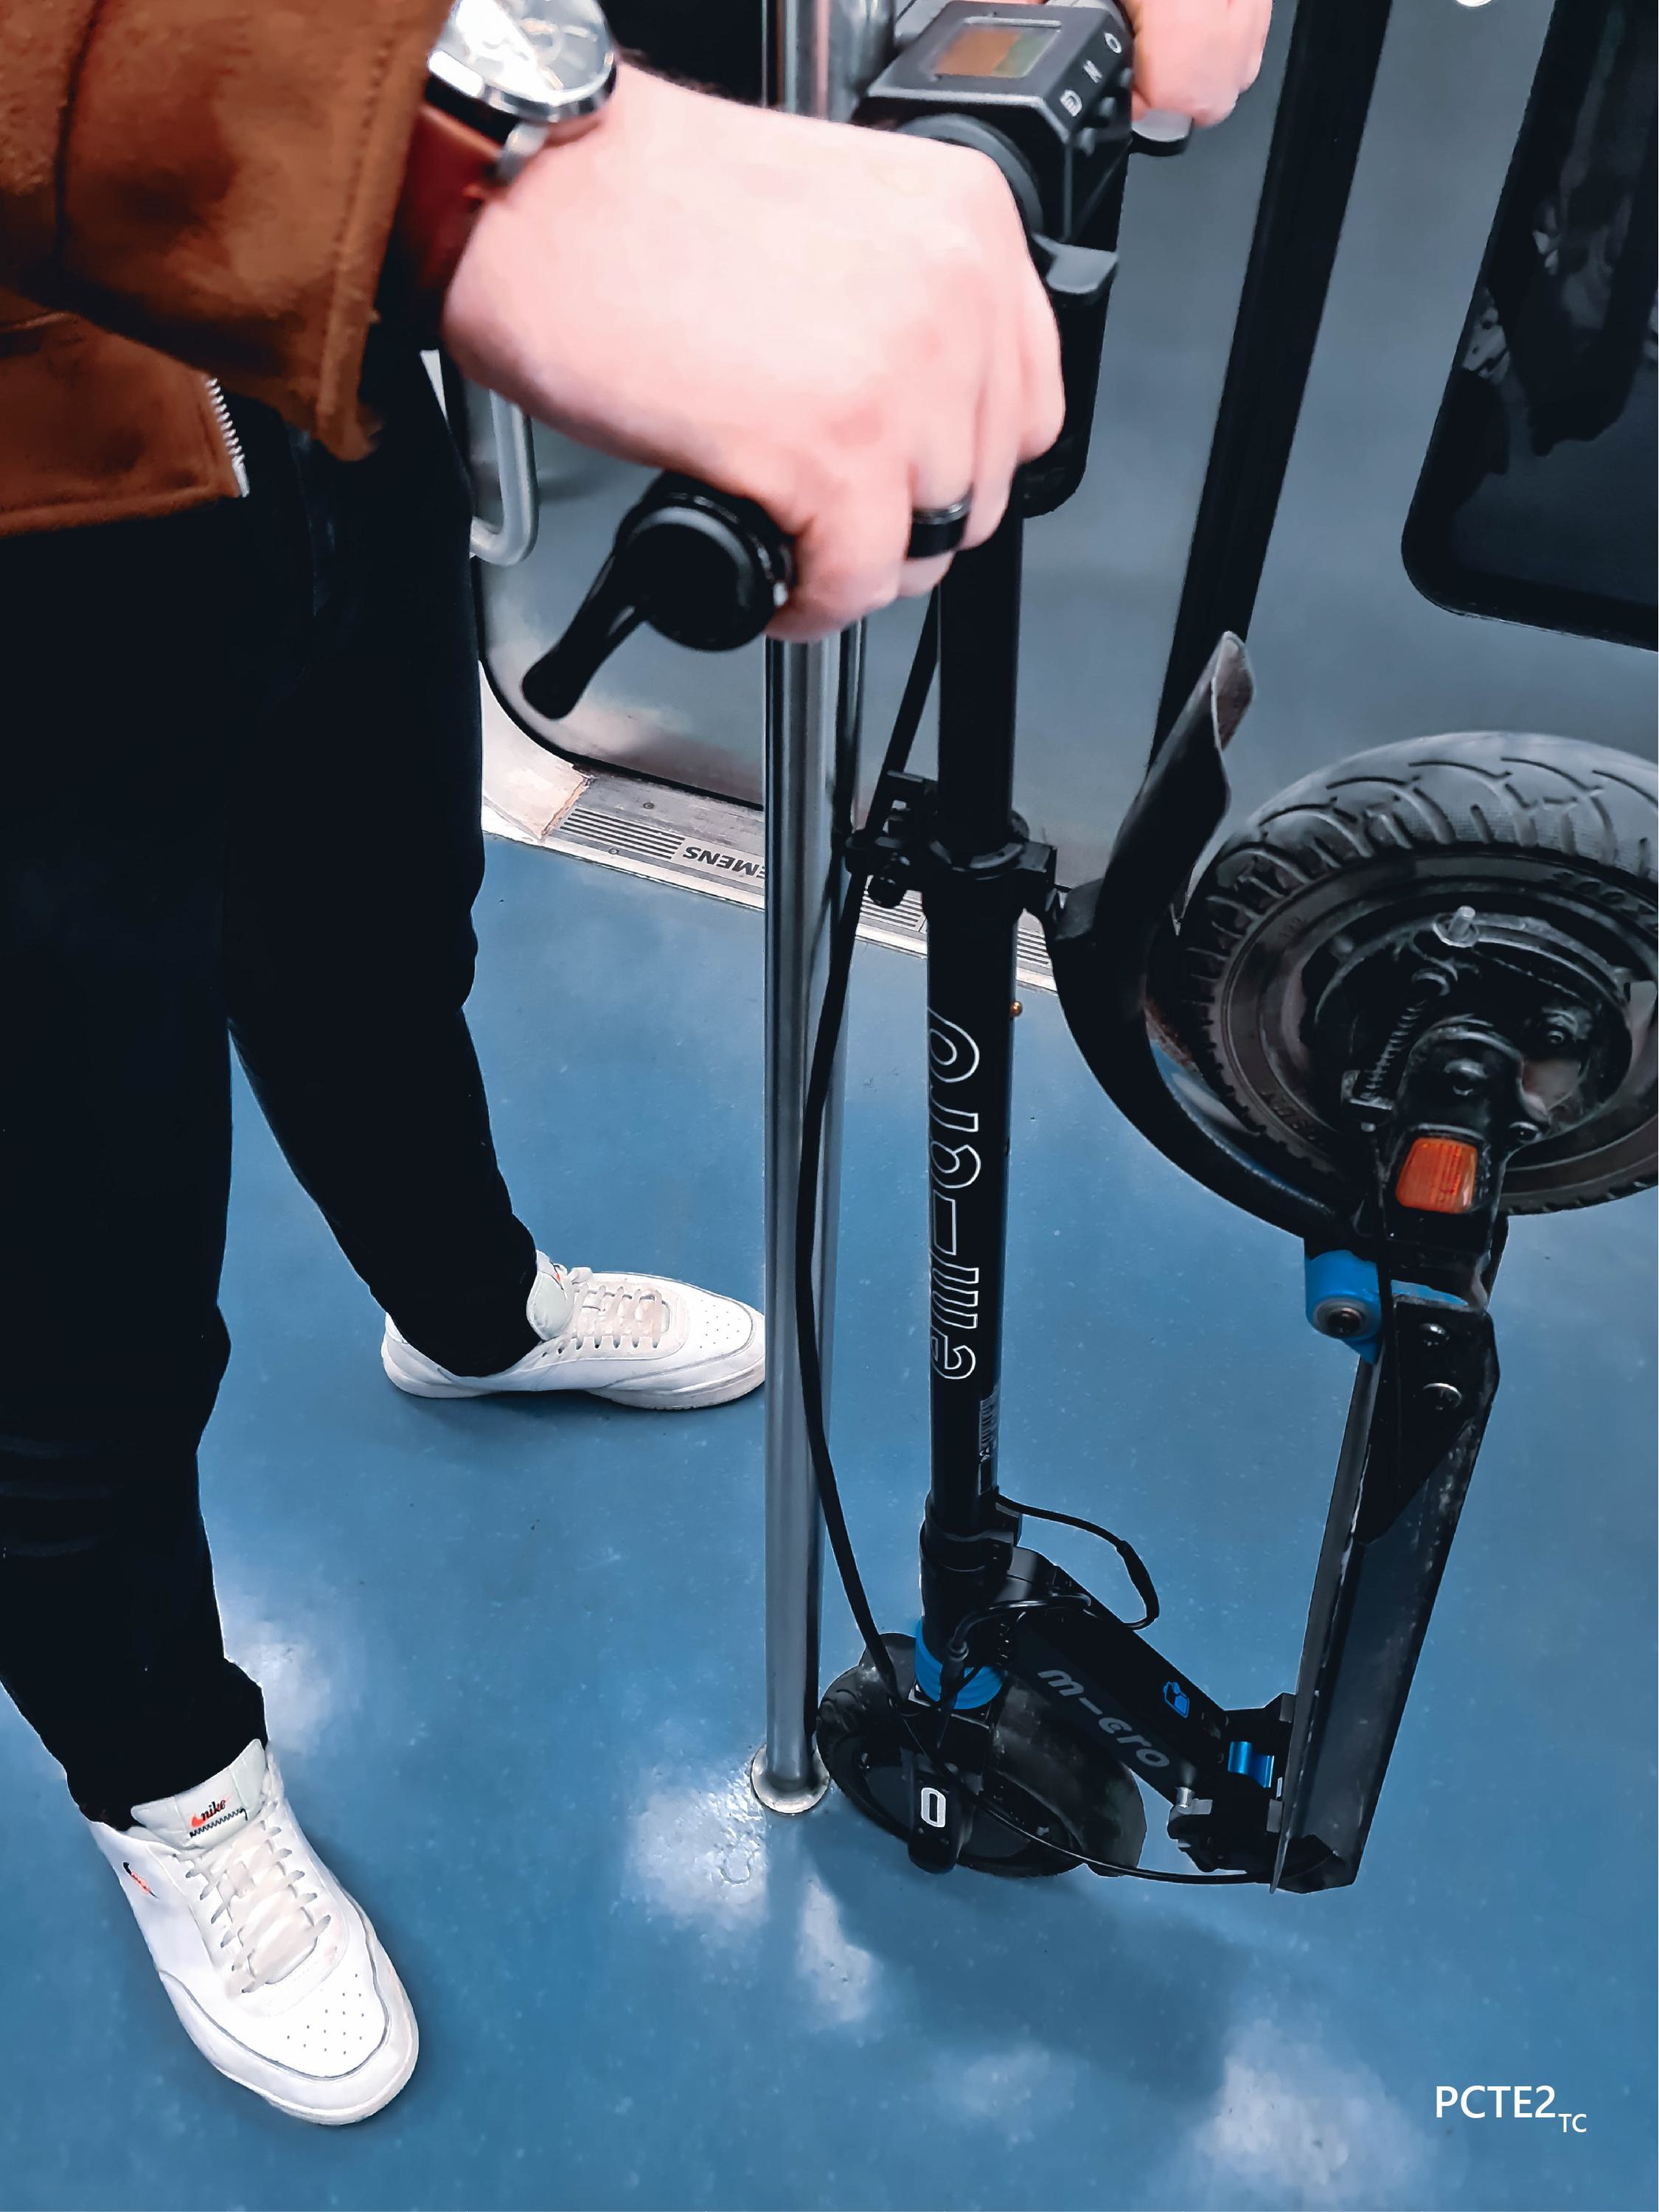
\includegraphics[width=0.5\columnwidth]{src/Figures/Annexes/Extrait_Video_PCTE2_TC_2.jpg}}
        \vspace{5pt}
        \begin{flushright}\scriptsize{
        Author: \textcolor{blue}{Dylan Moinse (2022)}
        }\end{flushright}
    \end{figure}
    
    % PCTE2 Photo TC 3
    \begin{figure}[h!]\vspace*{4pt}
        \caption*{Excerpt No. 3 from the video during the metro trip (\(PCTE^{TC}_{2}\))}
        \centerline{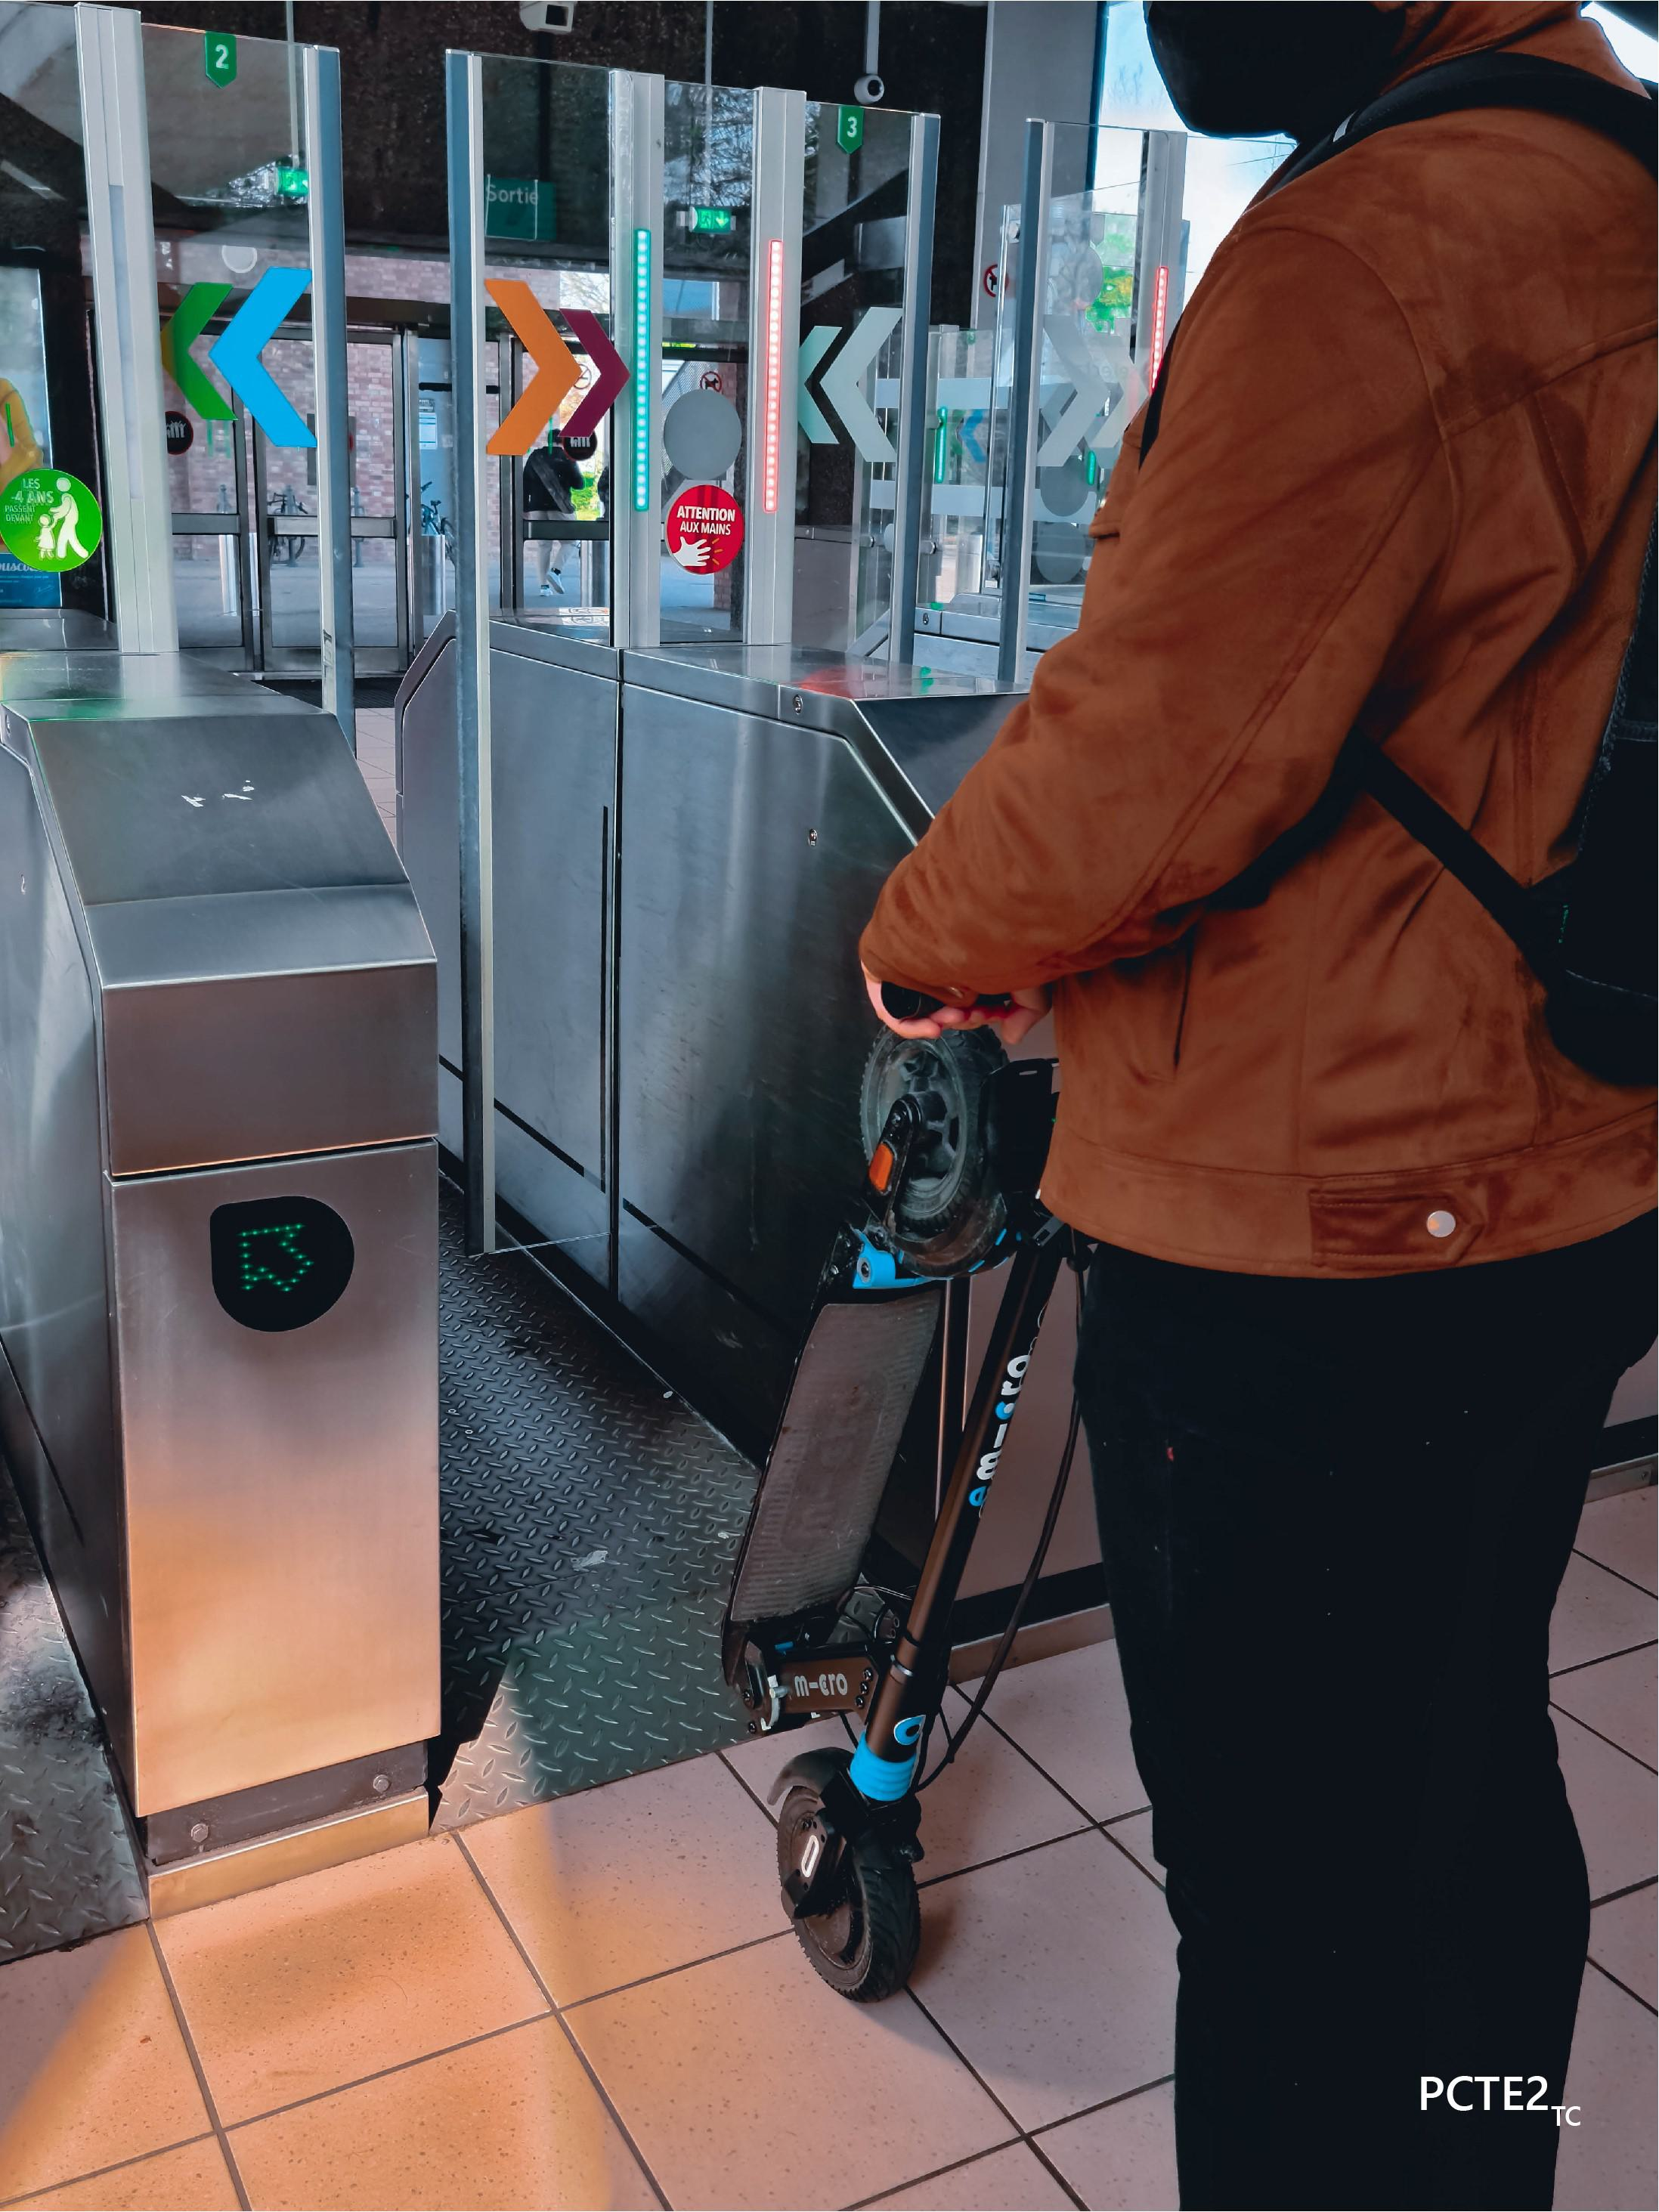
\includegraphics[width=0.5\columnwidth]{src/Figures/Annexes/Extrait_Video_PCTE2_TC_3.jpg}}
        \vspace{5pt}
        \begin{flushright}\scriptsize{
        Author: \textcolor{blue}{Dylan Moinse (2022)}
        }\end{flushright}
    \end{figure}

    % Photos PCTE2 egress
\subsubsection{Selection of Images Extracted During the Egress Trip}

    % PCTE2 Photo Egress 1
    \begin{figure}[h!]\vspace*{4pt}
        \caption*{Excerpt No. 1 from the video during the egress segment (\(PCTE^{E}_{2}\))}
        \centerline{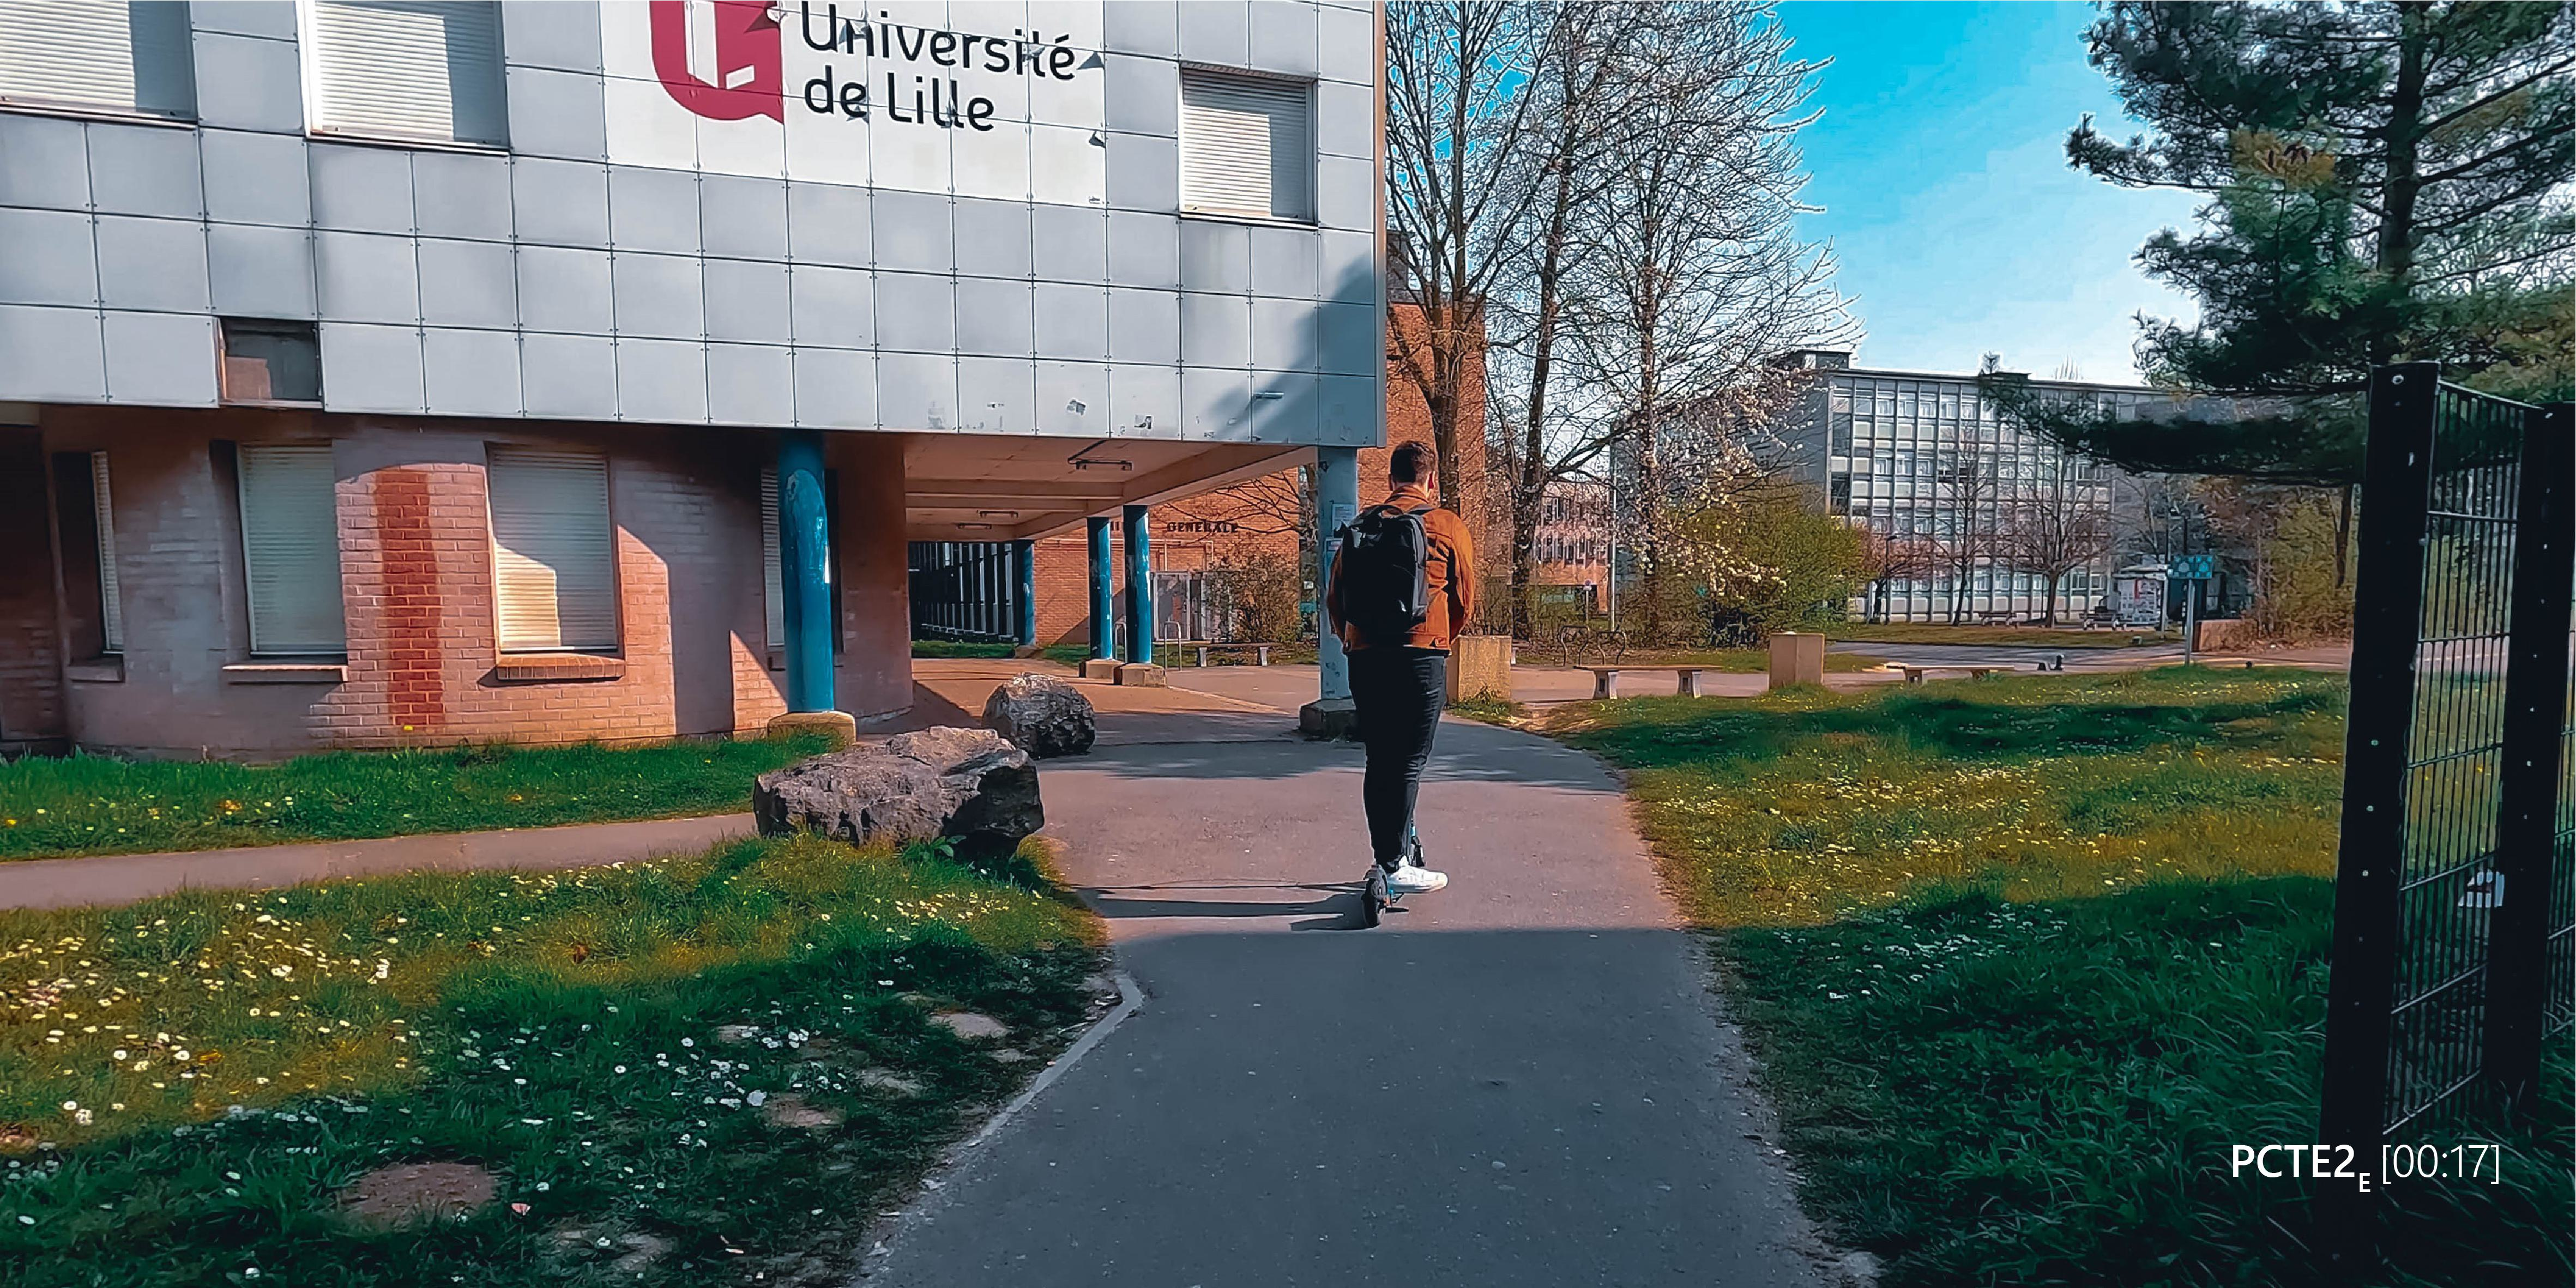
\includegraphics[width=0.75\columnwidth]{src/Figures/Annexes/Extrait_Video_PCTE2_Egress_1.jpg}}
        \vspace{5pt}
        \begin{flushright}\scriptsize{
        Author: \textcolor{blue}{Dylan Moinse (2022)}
        }\end{flushright}
    \end{figure}

    % PCTE2 Photo Egress 2
    \begin{figure}[h!]\vspace*{4pt}
        \caption*{Excerpt No. 2 from the video during the egress segment (\(PCTE^{E}_{2}\))}
        \centerline{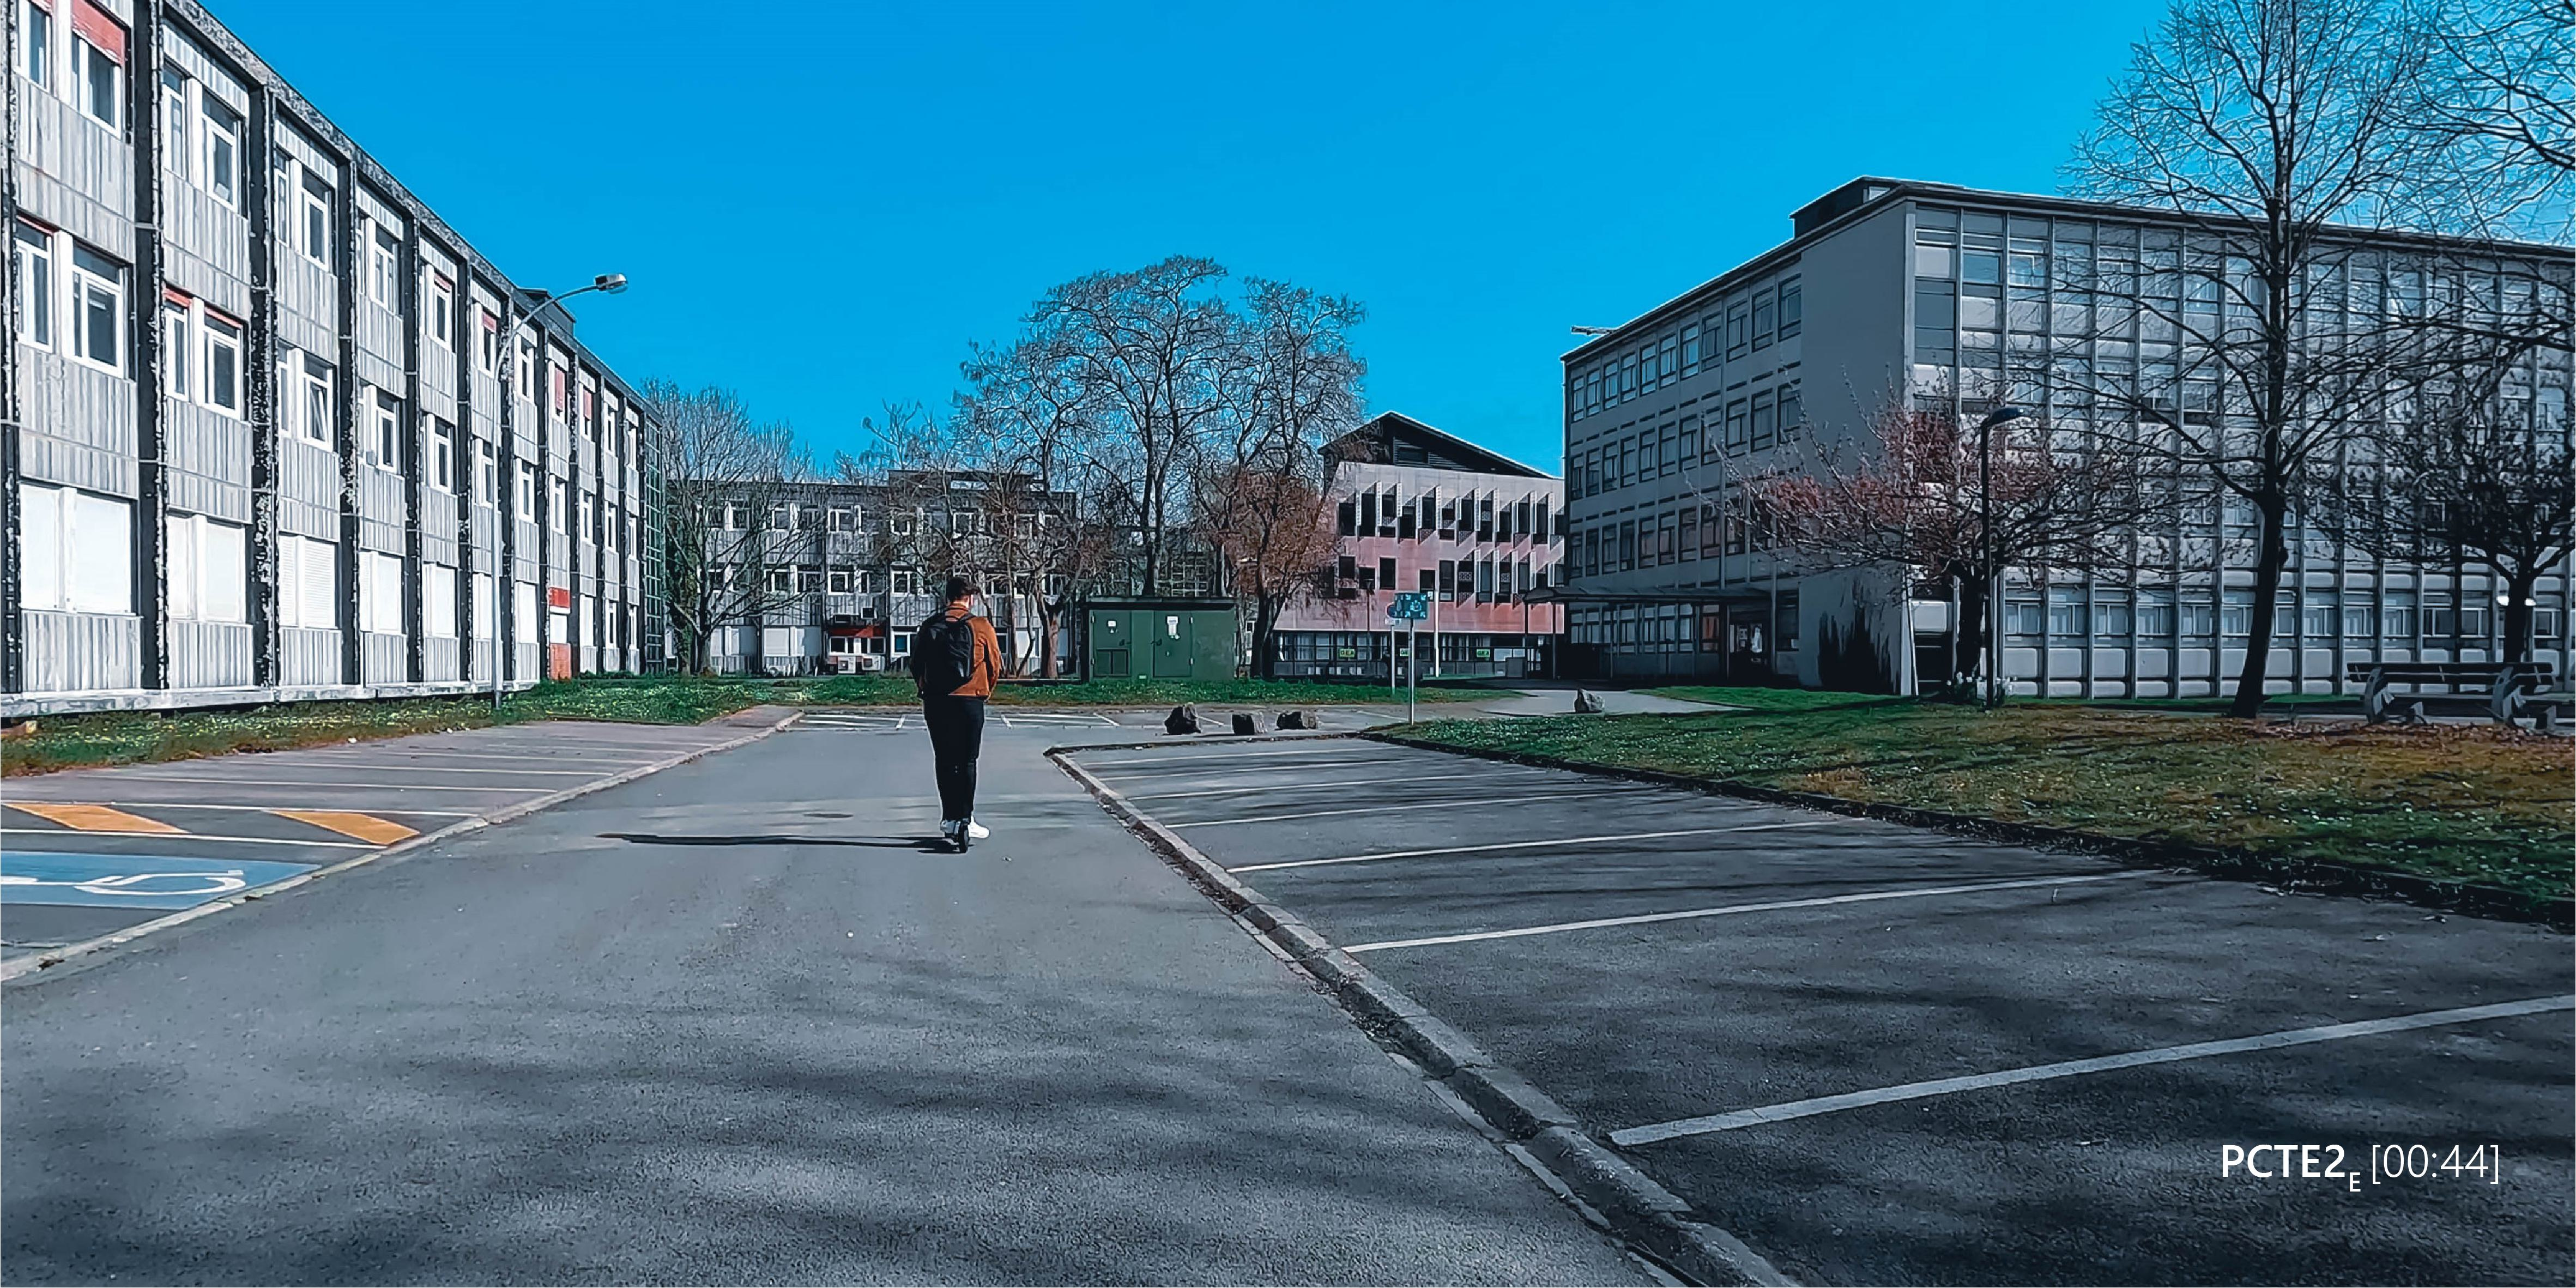
\includegraphics[width=0.75\columnwidth]{src/Figures/Annexes/Extrait_Video_PCTE2_Egress_2.jpg}}
        \vspace{5pt}
        \begin{flushright}\scriptsize{
        Author: \textcolor{blue}{Dylan Moinse (2022)}
        }\end{flushright}
    \end{figure}

    % PCTE2 Photo Egress 3
    \begin{figure}[h!]\vspace*{4pt}
        \caption*{Excerpt No. 3 from the video during the egress segment (\(PCTE^{E}_{2}\))}
        \centerline{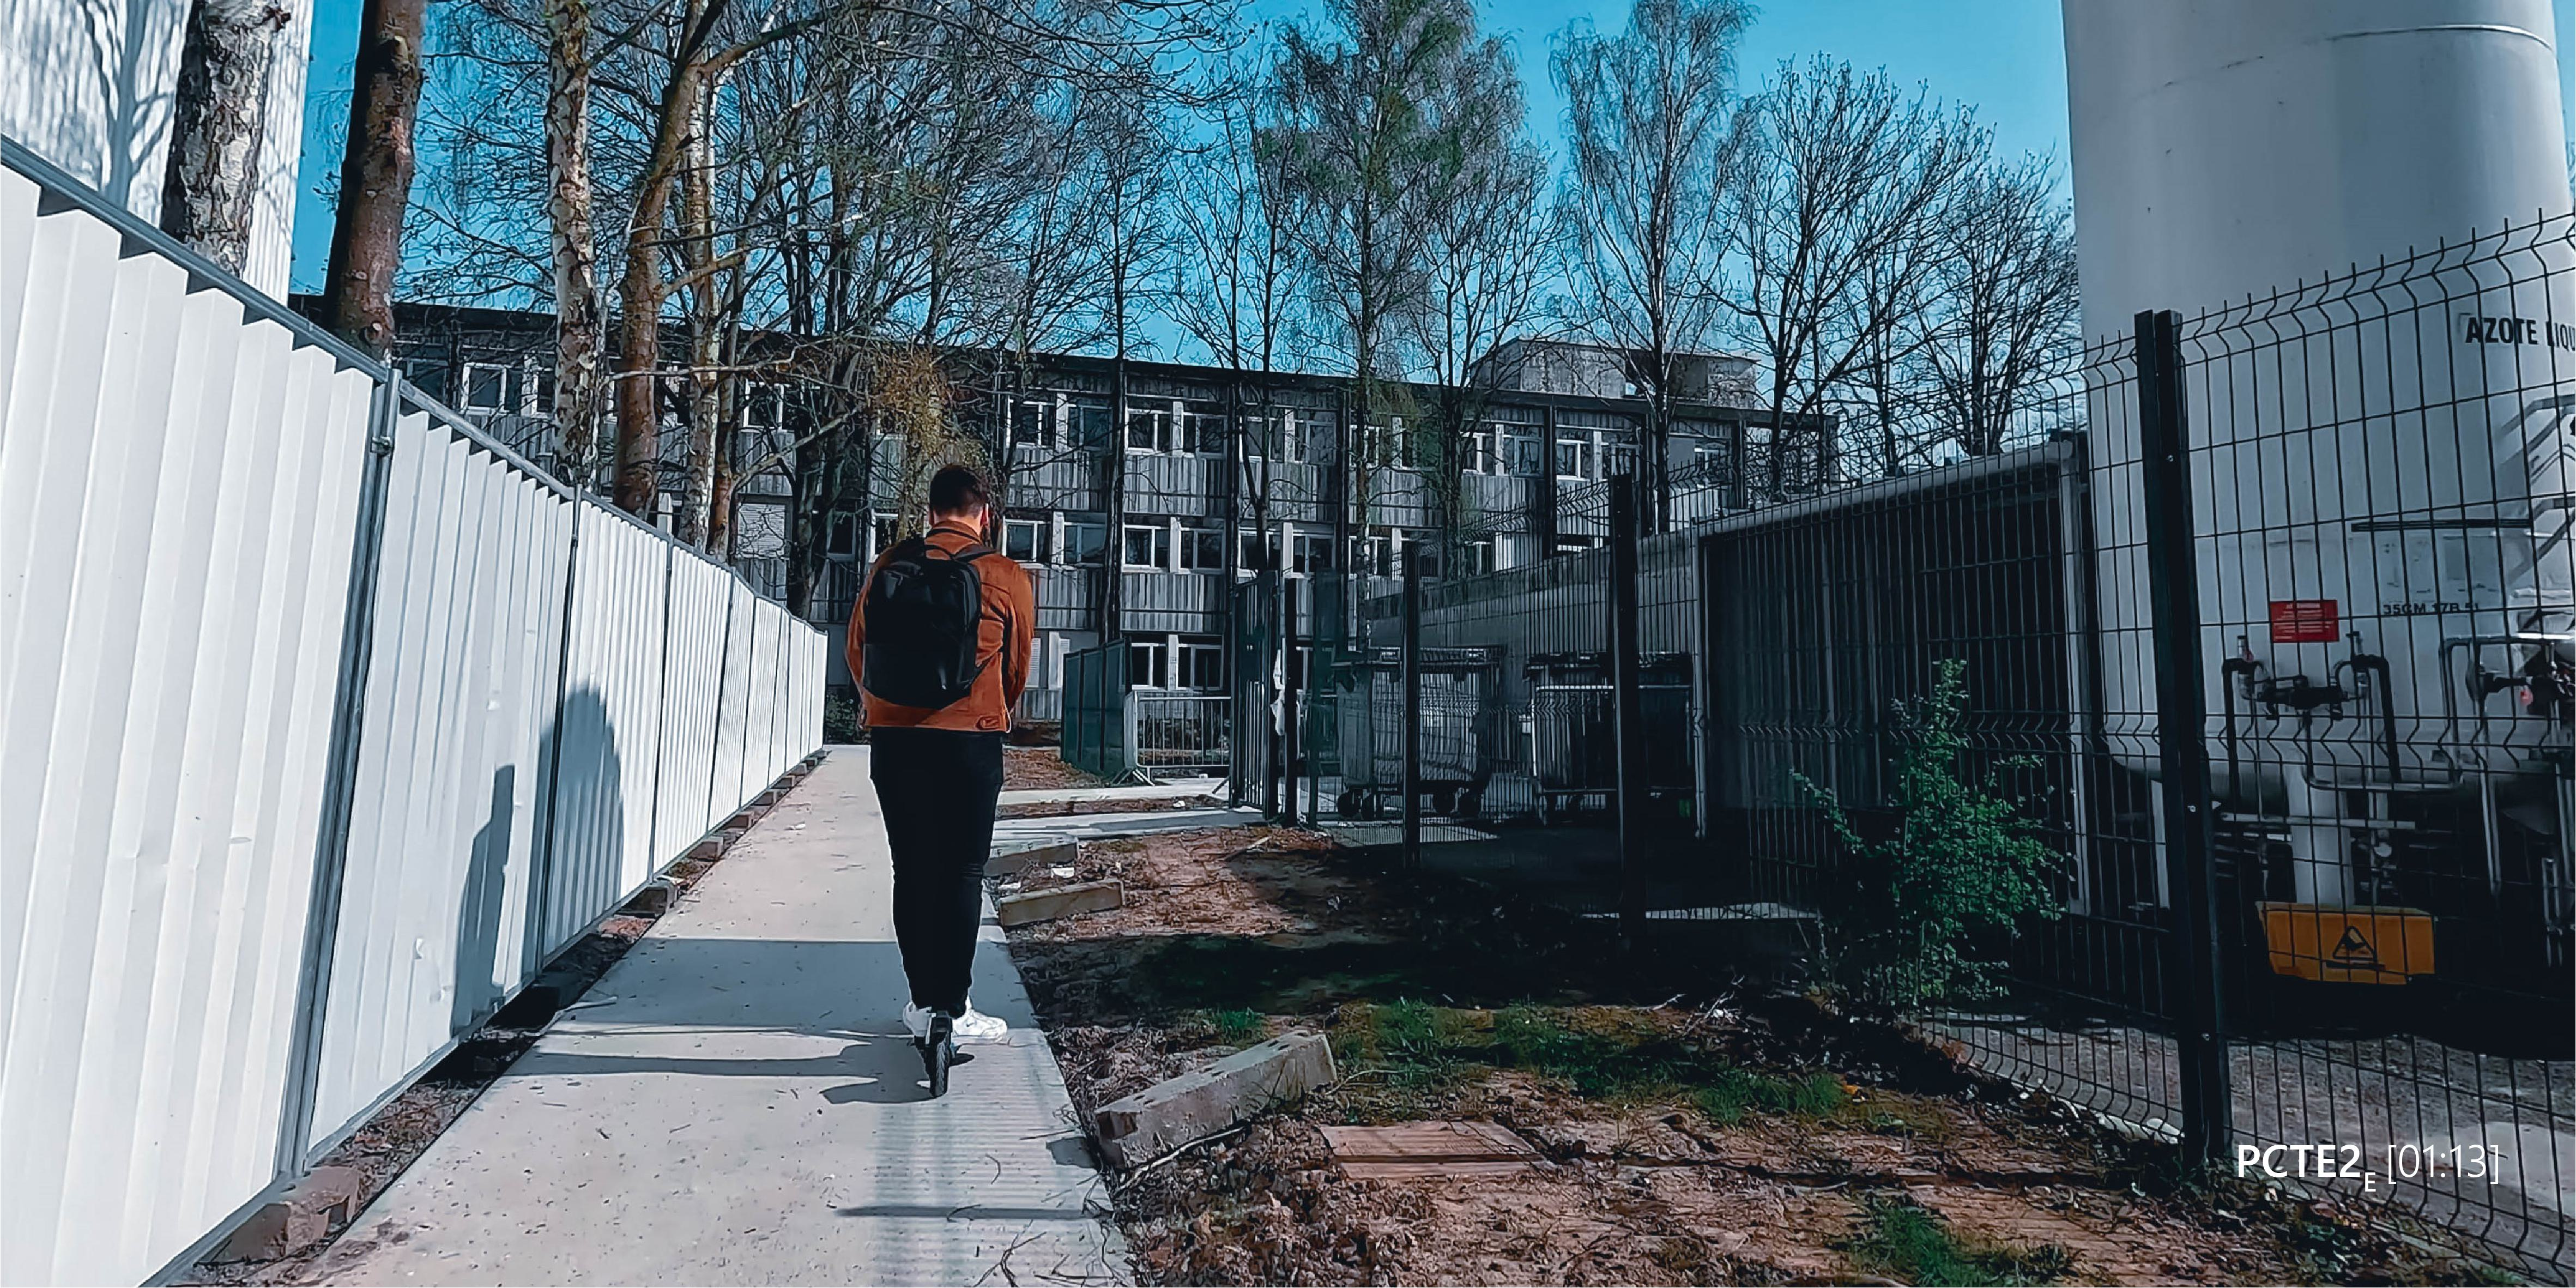
\includegraphics[width=0.75\columnwidth]{src/Figures/Annexes/Extrait_Video_PCTE2_Egress_3.jpg}}
        \vspace{5pt}
        \begin{flushright}\scriptsize{
        Author: \textcolor{blue}{Dylan Moinse (2022)}
        }\end{flushright}
    \end{figure}

    % PCTE2 Photo Egress 4
    \begin{figure}[h!]\vspace*{4pt}
        \caption*{Excerpt No. 4 from the video during the egress segment (\(PCTE^{E}_{2}\))}
        \centerline{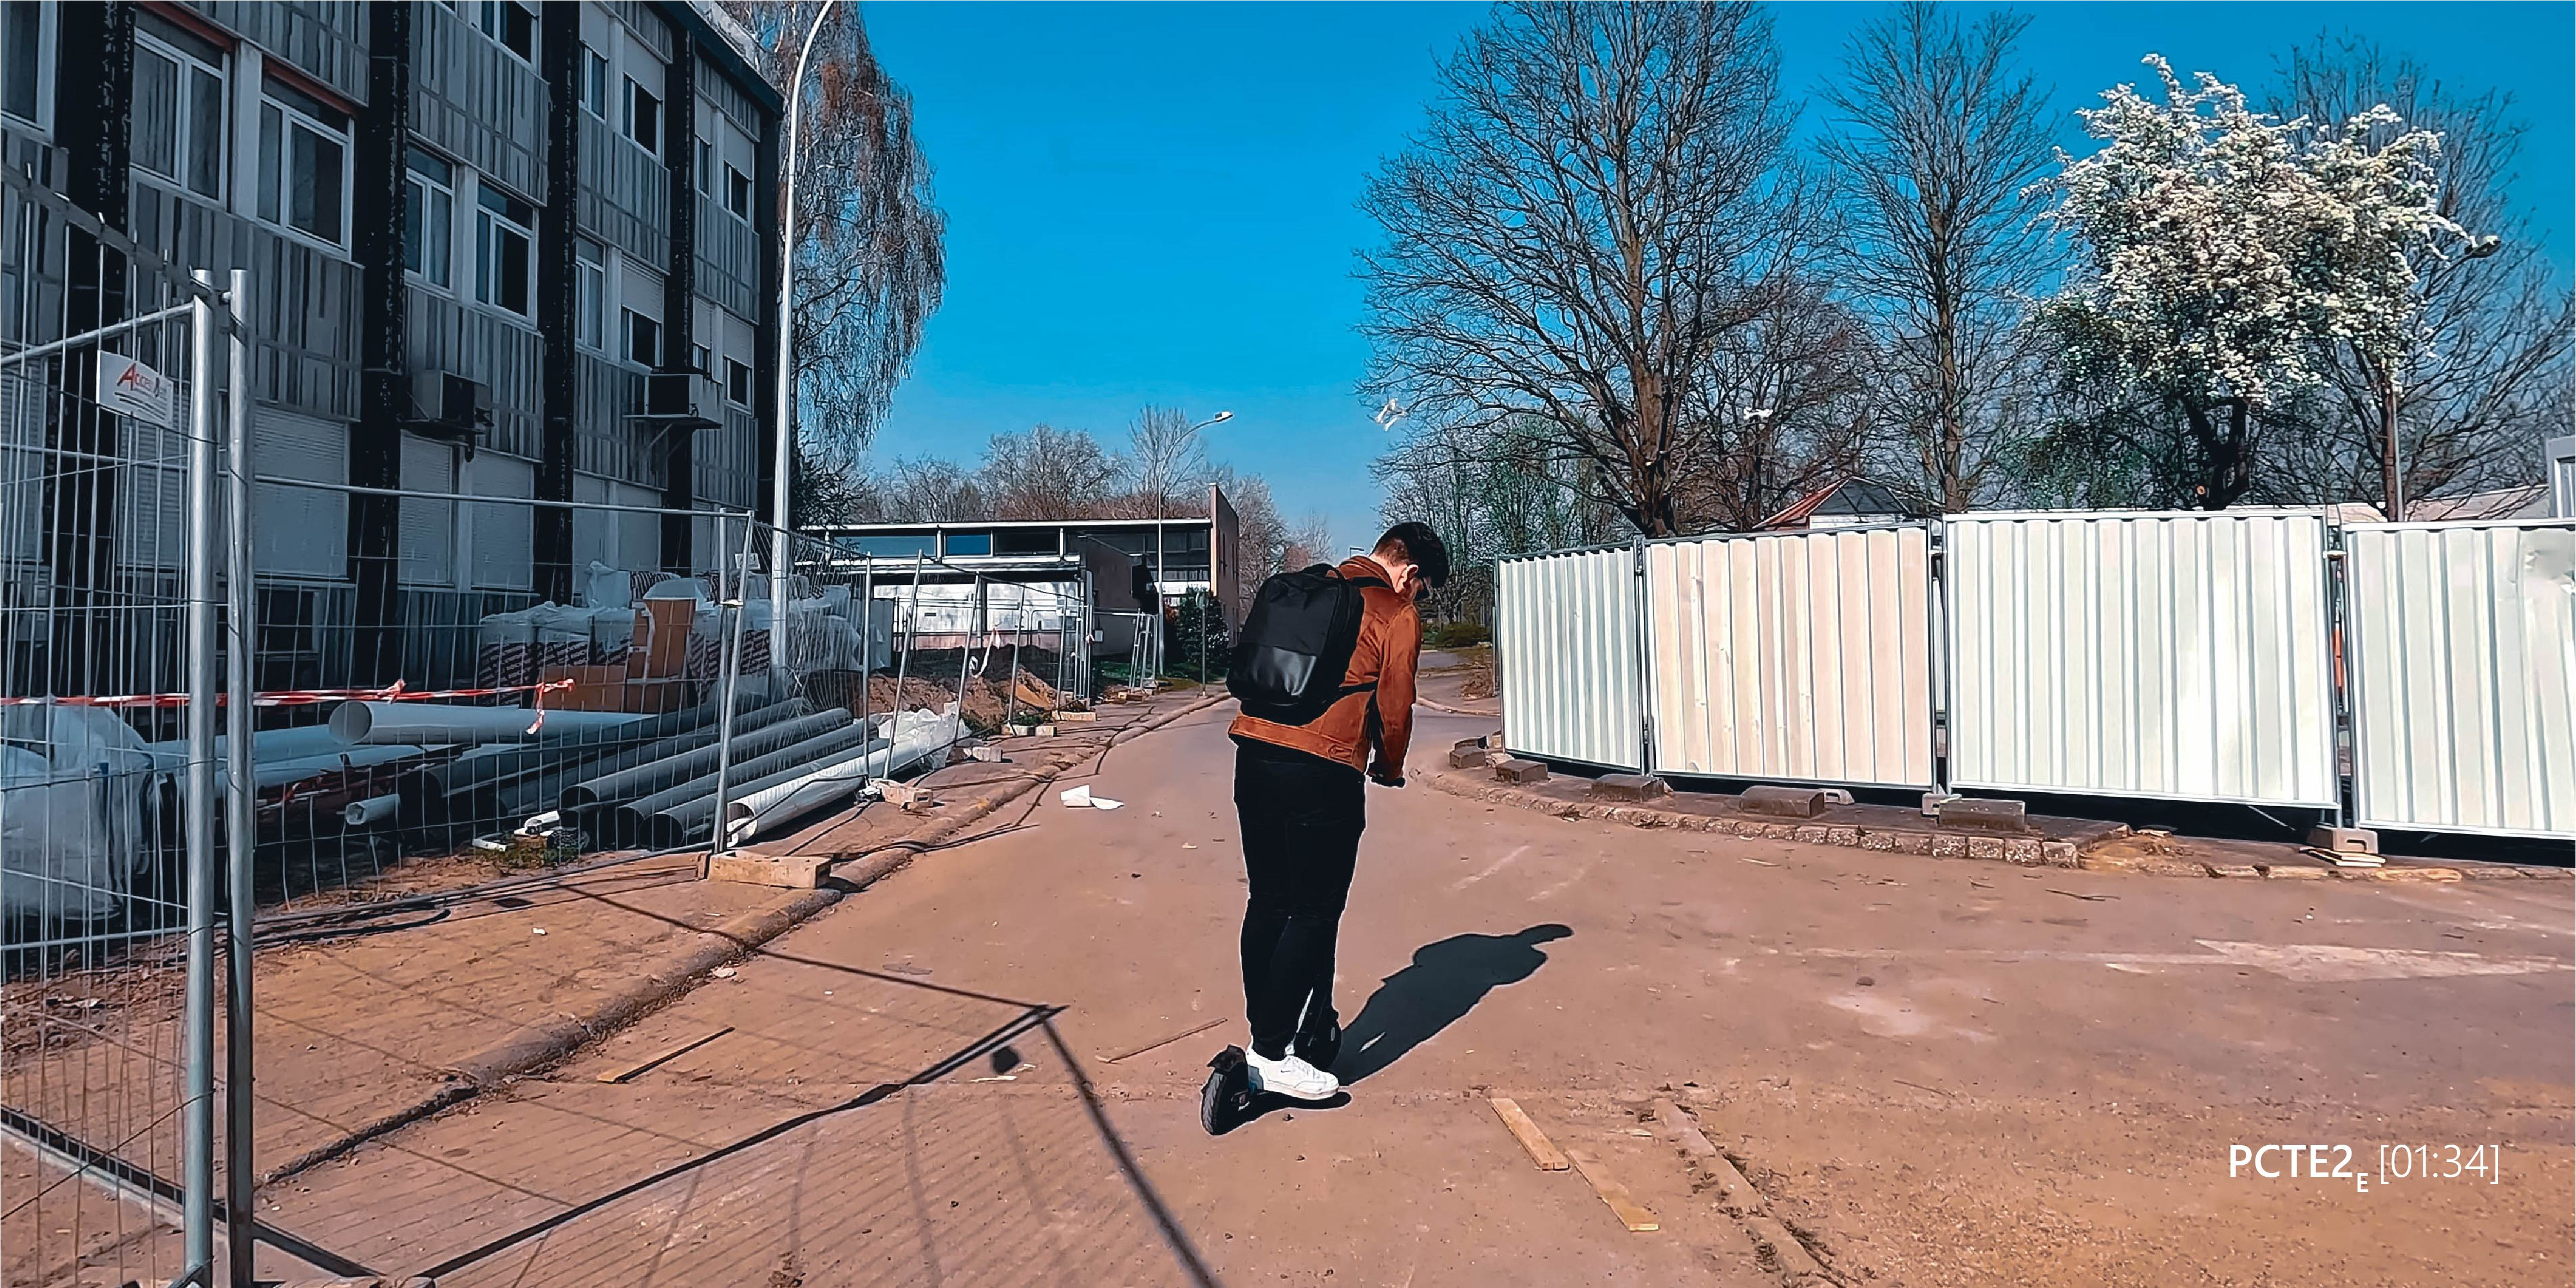
\includegraphics[width=0.75\columnwidth]{src/Figures/Annexes/Extrait_Video_PCTE2_Egress_4.jpg}}
        \vspace{5pt}
        \begin{flushright}\scriptsize{
        Author: \textcolor{blue}{Dylan Moinse (2022)}
        }\end{flushright}
    \end{figure}

    % PCTE2 Photo Egress 5
    \begin{figure}[h!]\vspace*{4pt}
        \caption*{Excerpt No. 5 from the video during the egress segment (\(PCTE^{E}_{2}\))}
        \centerline{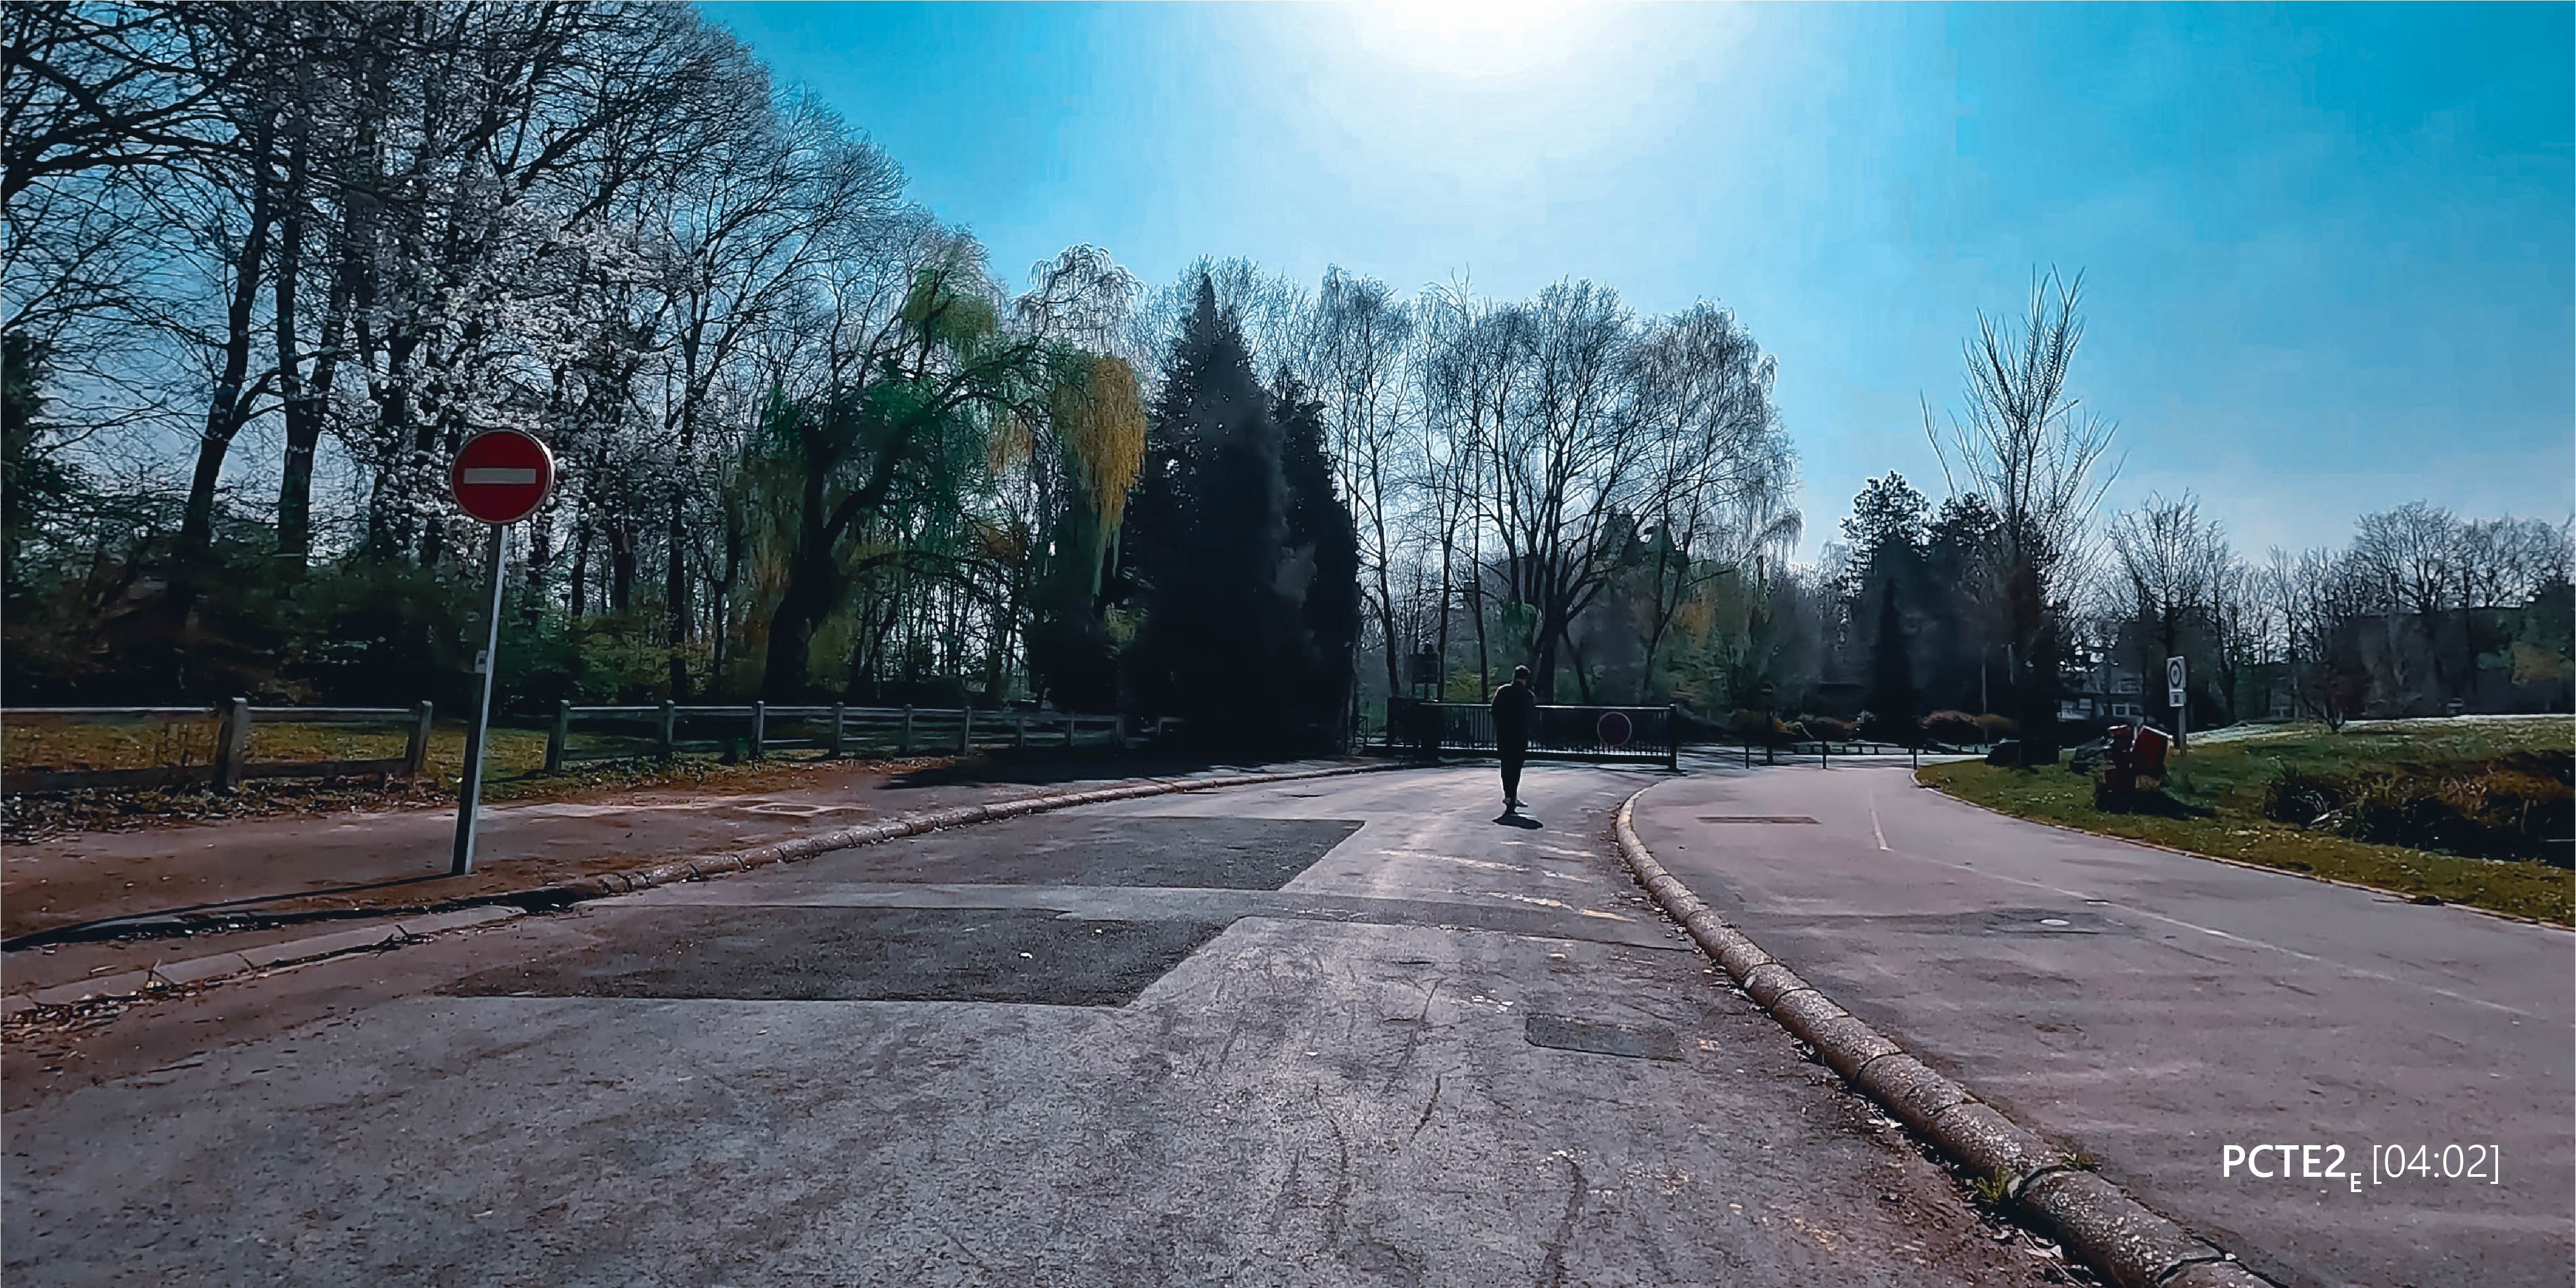
\includegraphics[width=0.75\columnwidth]{src/Figures/Annexes/Extrait_Video_PCTE2_Egress_5.jpg}}
        \vspace{5pt}
        \begin{flushright}\scriptsize{
        Author: \textcolor{blue}{Dylan Moinse (2022)}
        }\end{flushright}
    \end{figure}

    % PCTE2 Photo Egress 6
    \begin{figure}[h!]\vspace*{4pt}
        \caption*{Excerpt No. 6 from the video during the egress segment (\(PCTE^{E}_{2}\))}
        \centerline{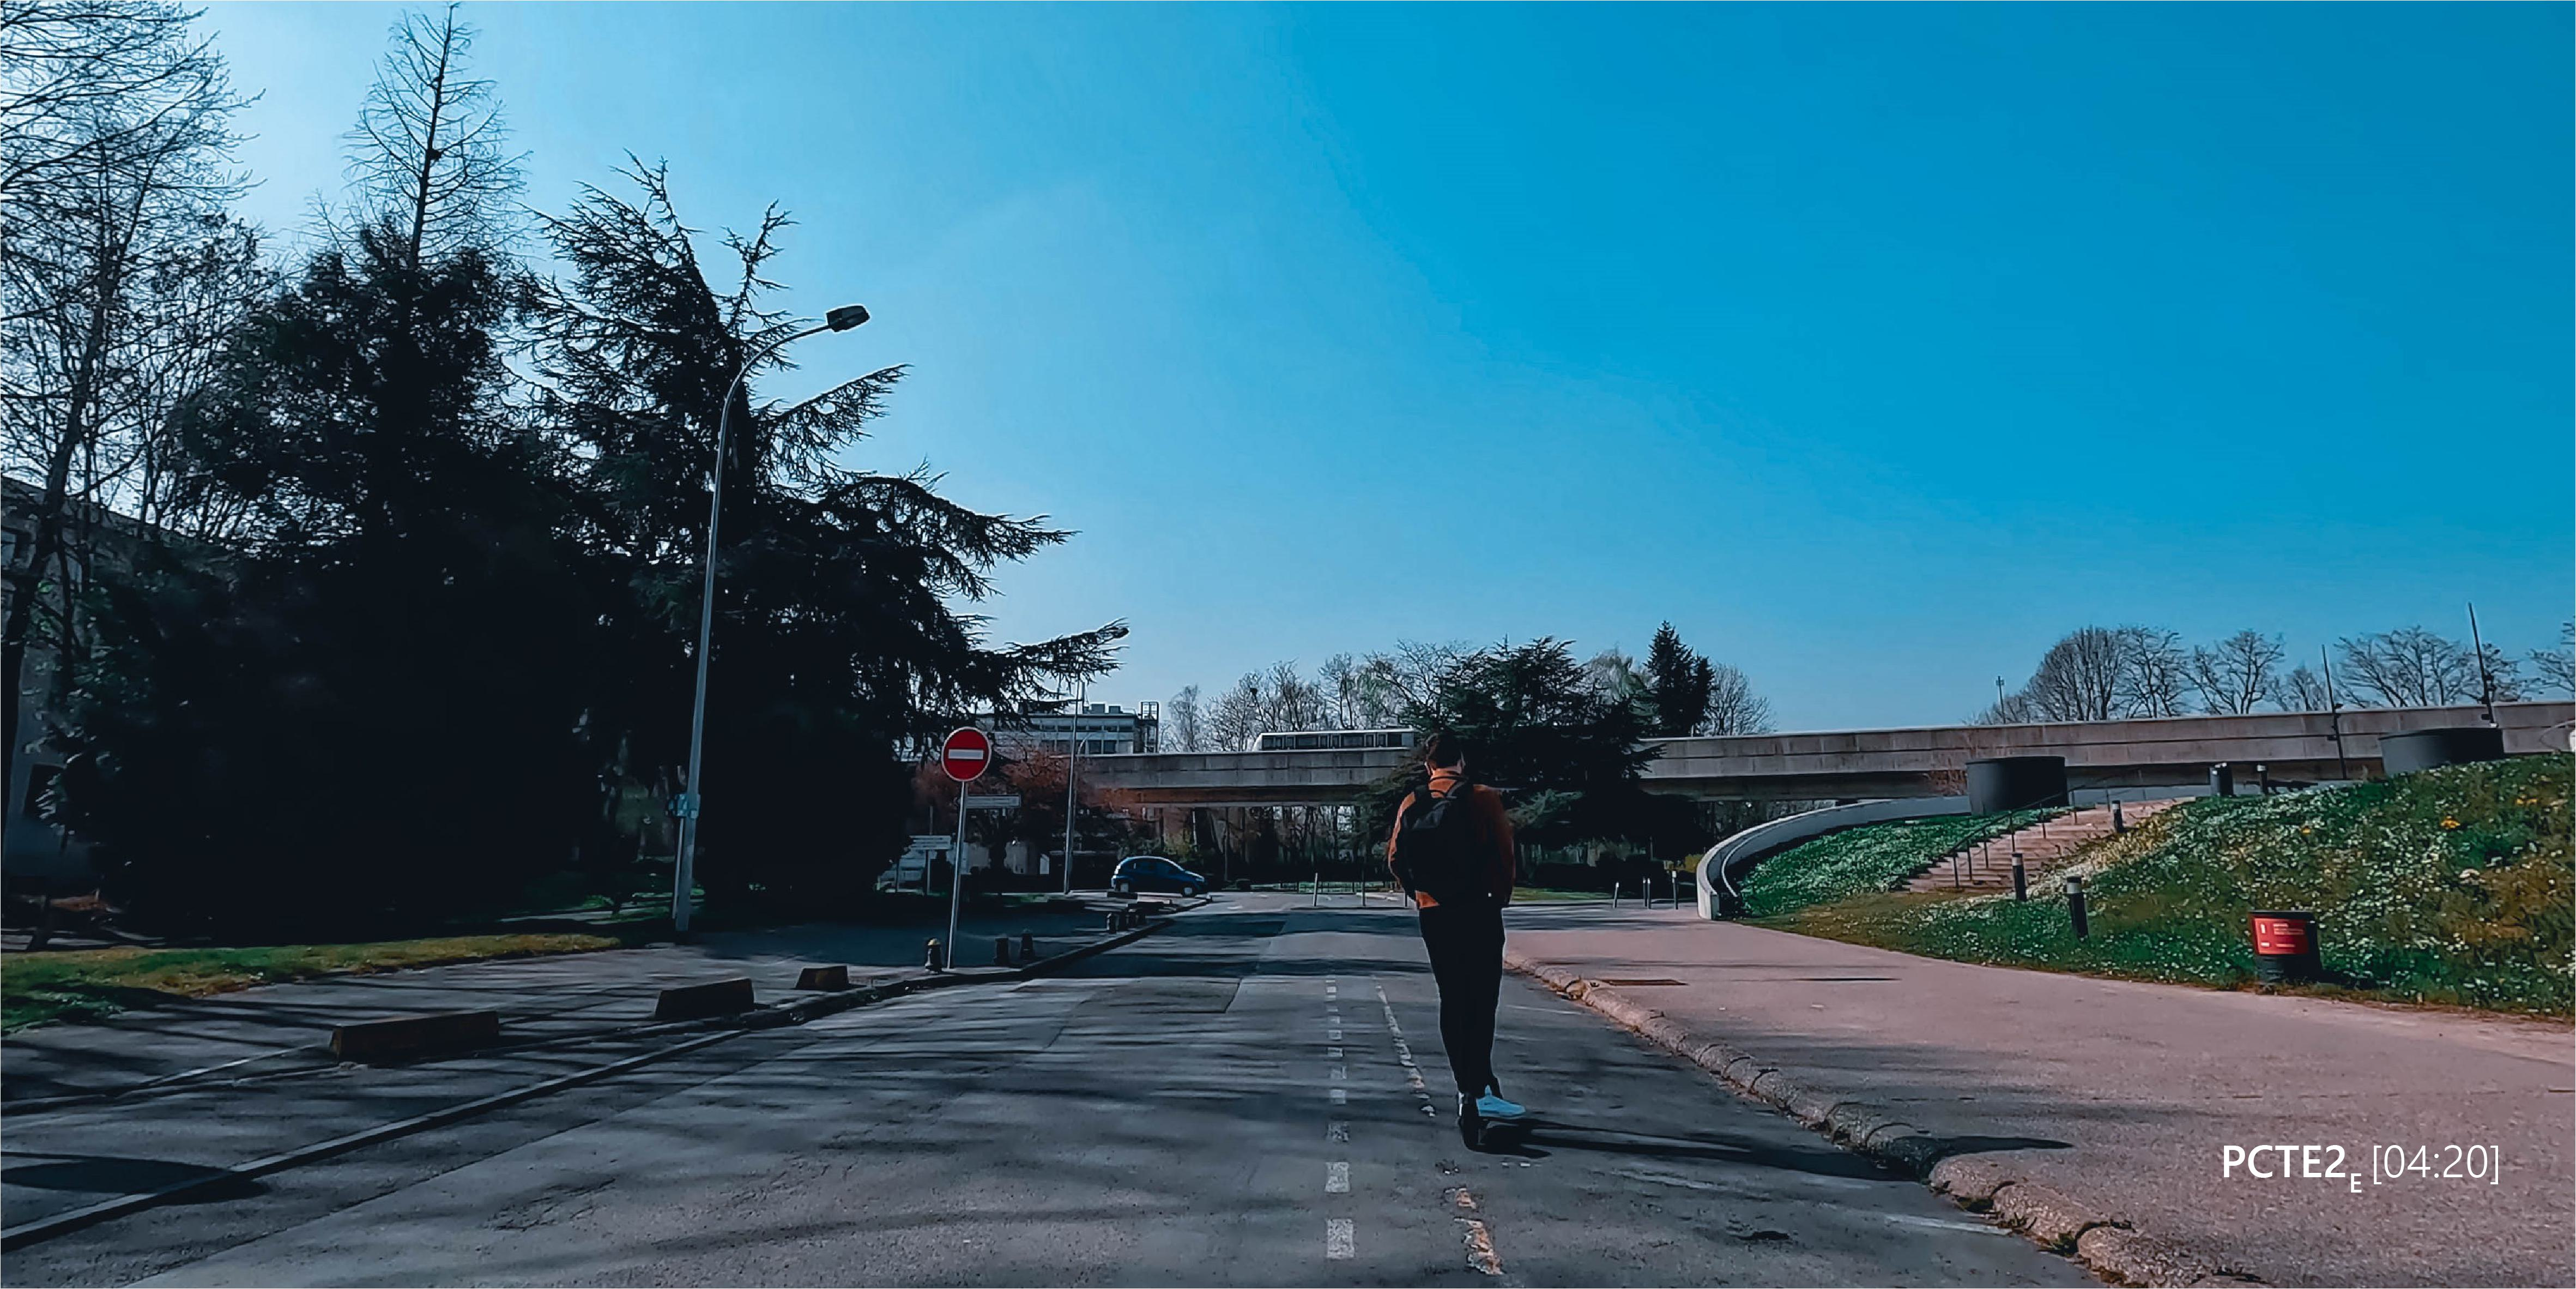
\includegraphics[width=0.75\columnwidth]{src/Figures/Annexes/Extrait_Video_PCTE2_Egress_6.jpg}}
        \vspace{5pt}
        \begin{flushright}\scriptsize{
        Author: \textcolor{blue}{Dylan Moinse (2022)}
        }\end{flushright}
    \end{figure}

    % PCTE2 Photo Egress 7
    \begin{figure}[h!]\vspace*{4pt}
        \caption*{Excerpt No. 7 from the video during the egress segment (\(PCTE^{E}_{2}\))}
        \centerline{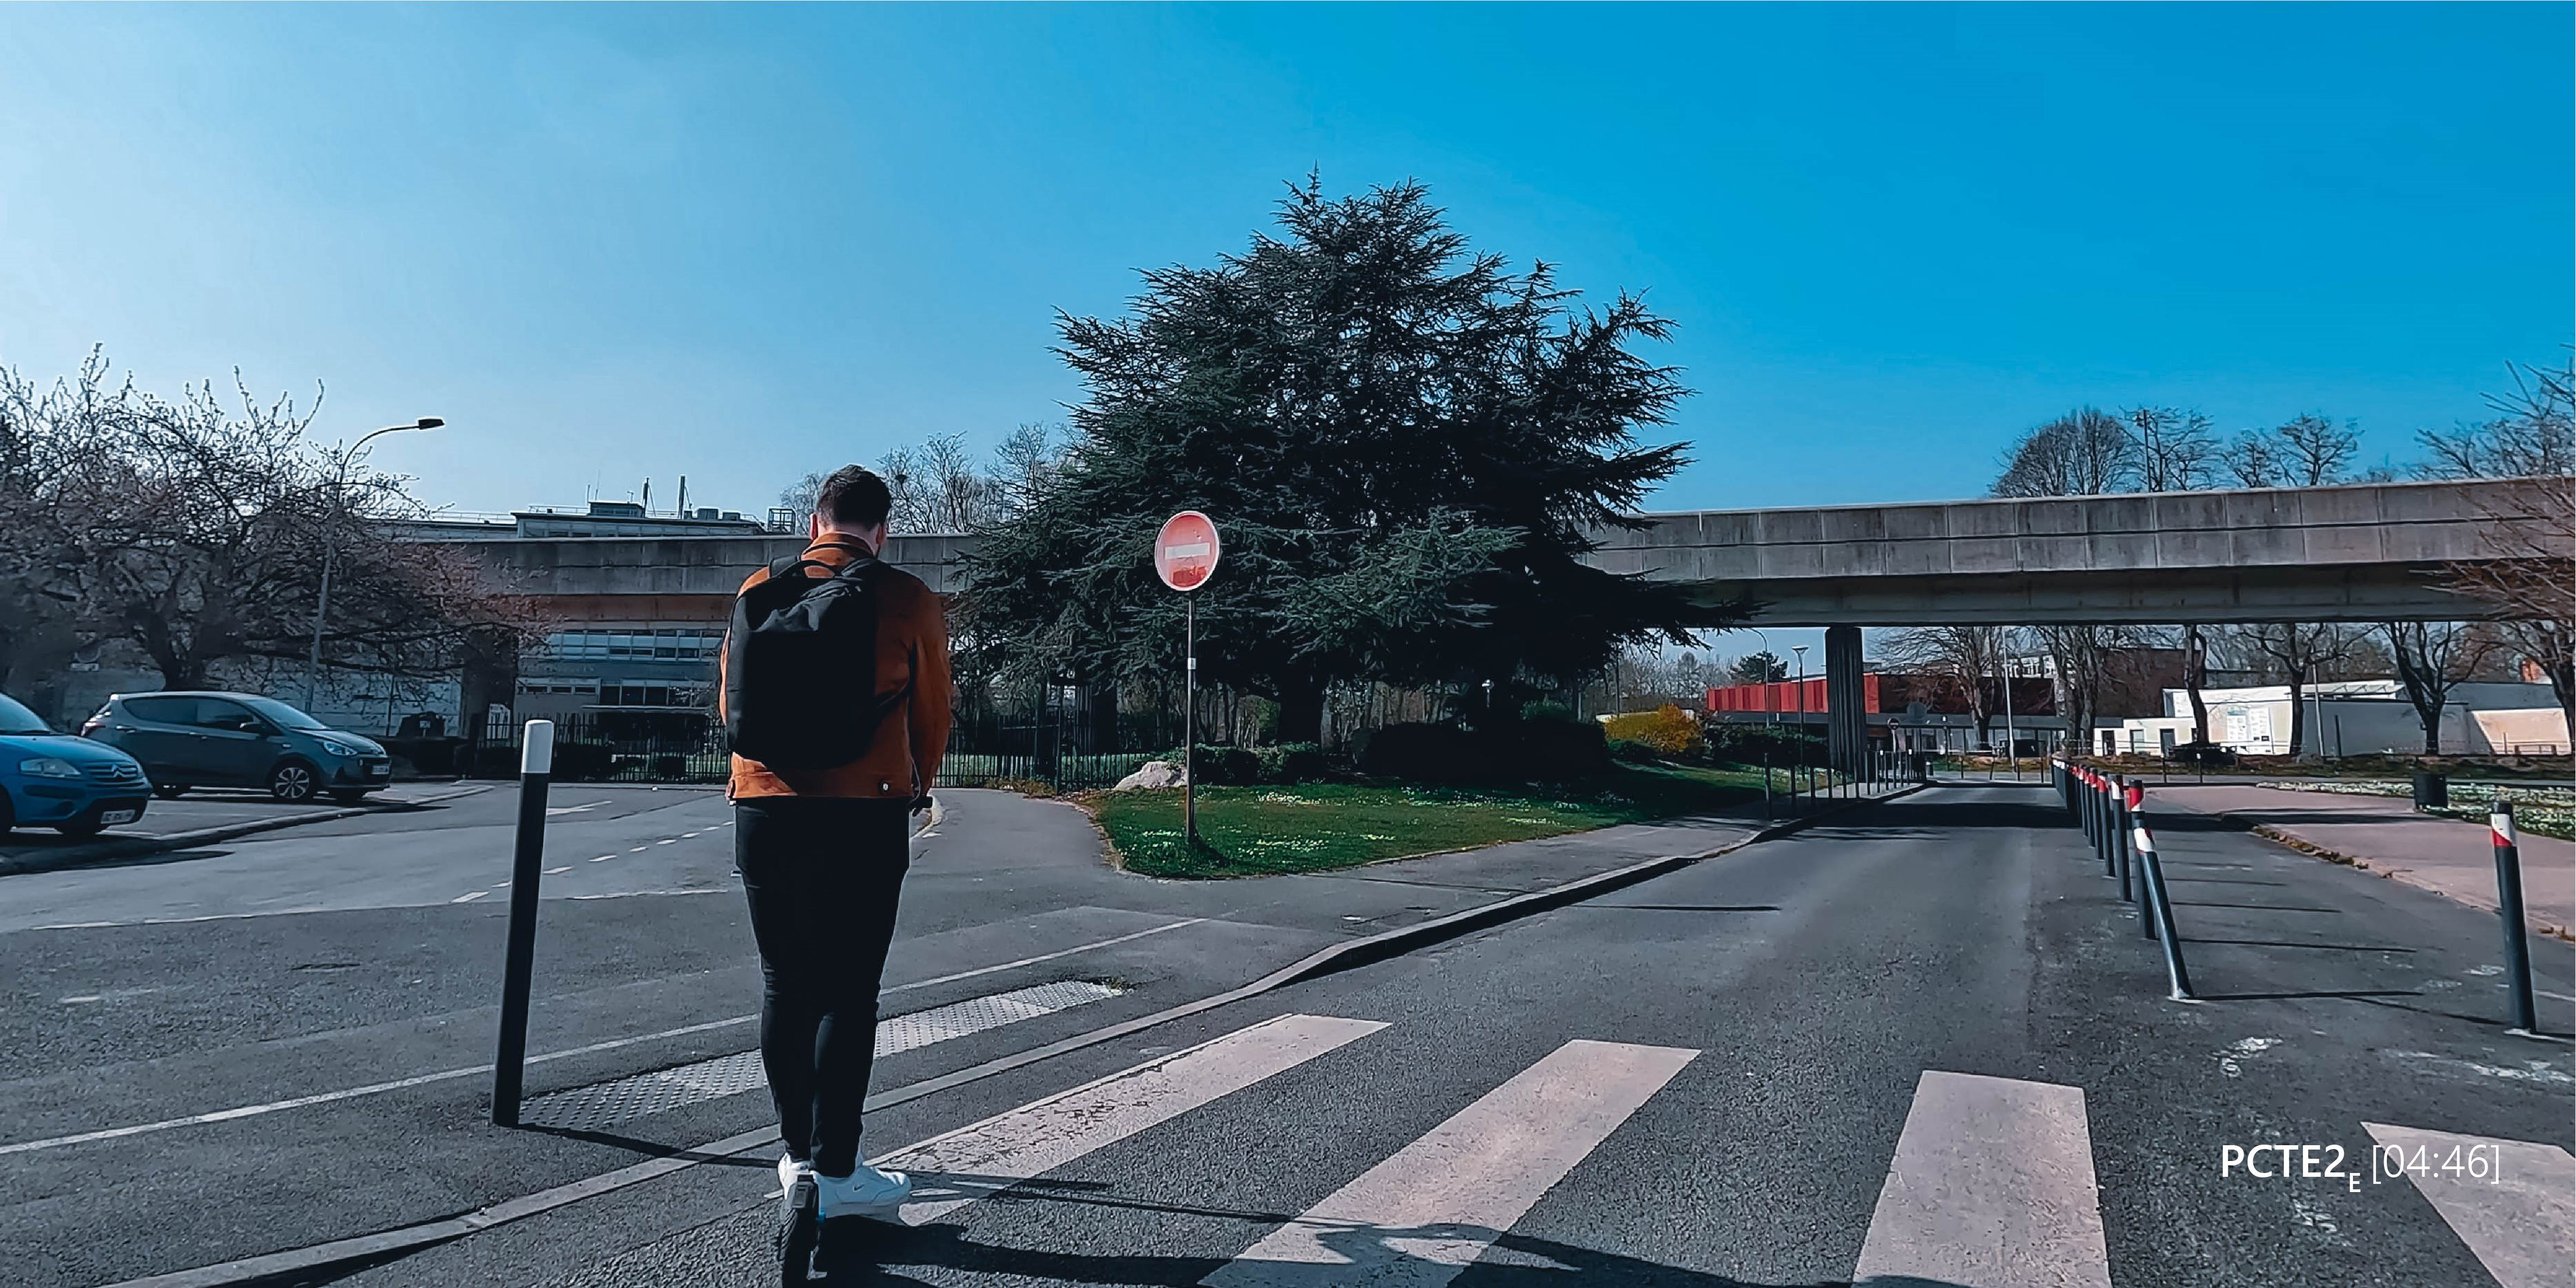
\includegraphics[width=0.75\columnwidth]{src/Figures/Annexes/Extrait_Video_PCTE2_Egress_7.jpg}}
        \vspace{5pt}
        \begin{flushright}\scriptsize{
        Author: \textcolor{blue}{Dylan Moinse (2022)}
        }\end{flushright}
    \end{figure}

    % PCTE2 Photo Egress 8
    \begin{figure}[h!]\vspace*{4pt}
        \caption*{Excerpt No. 8 from the video during the egress segment (\(PCTE^{E}_{2}\))}
        \centerline{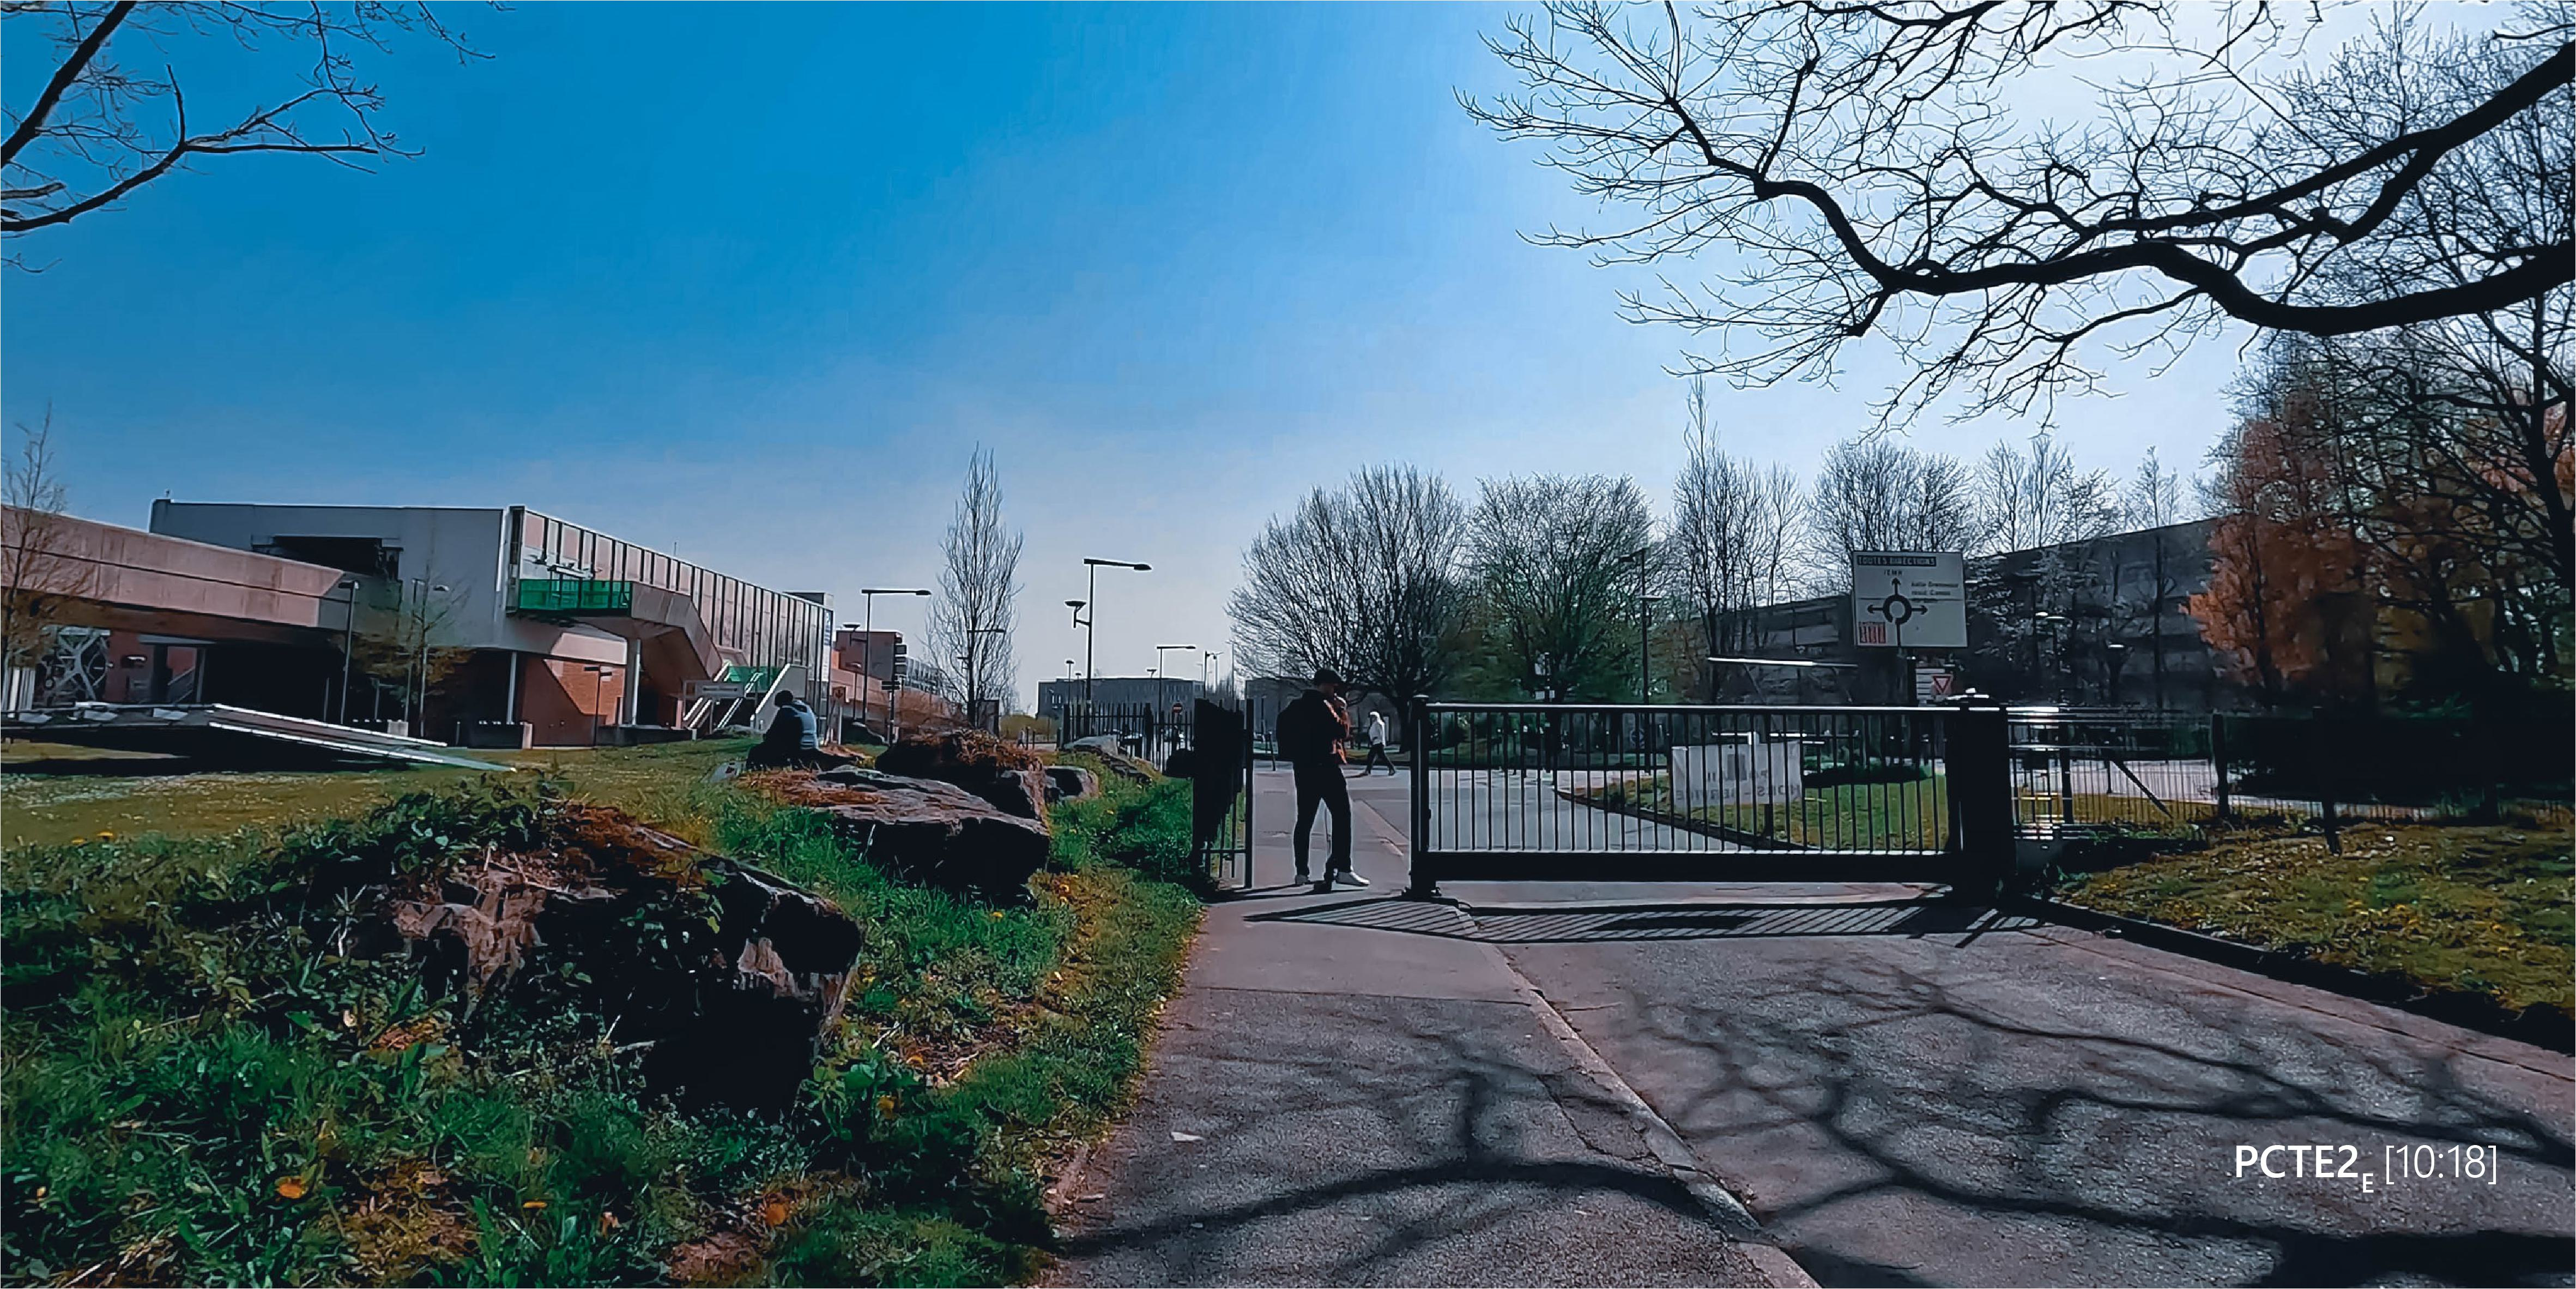
\includegraphics[width=0.75\columnwidth]{src/Figures/Annexes/Extrait_Video_PCTE2_Egress_8.jpg}}
        \vspace{5pt}
        \begin{flushright}\scriptsize{
        Author: \textcolor{blue}{Dylan Moinse (2022)}
        }\end{flushright}
    \end{figure}

    % PCTE2 Photo Egress 9
    \begin{figure}[h!]\vspace*{4pt}
        \caption*{Excerpt No. 9 from the video during the egress segment (\(PCTE^{E}_{2}\))}
        \centerline{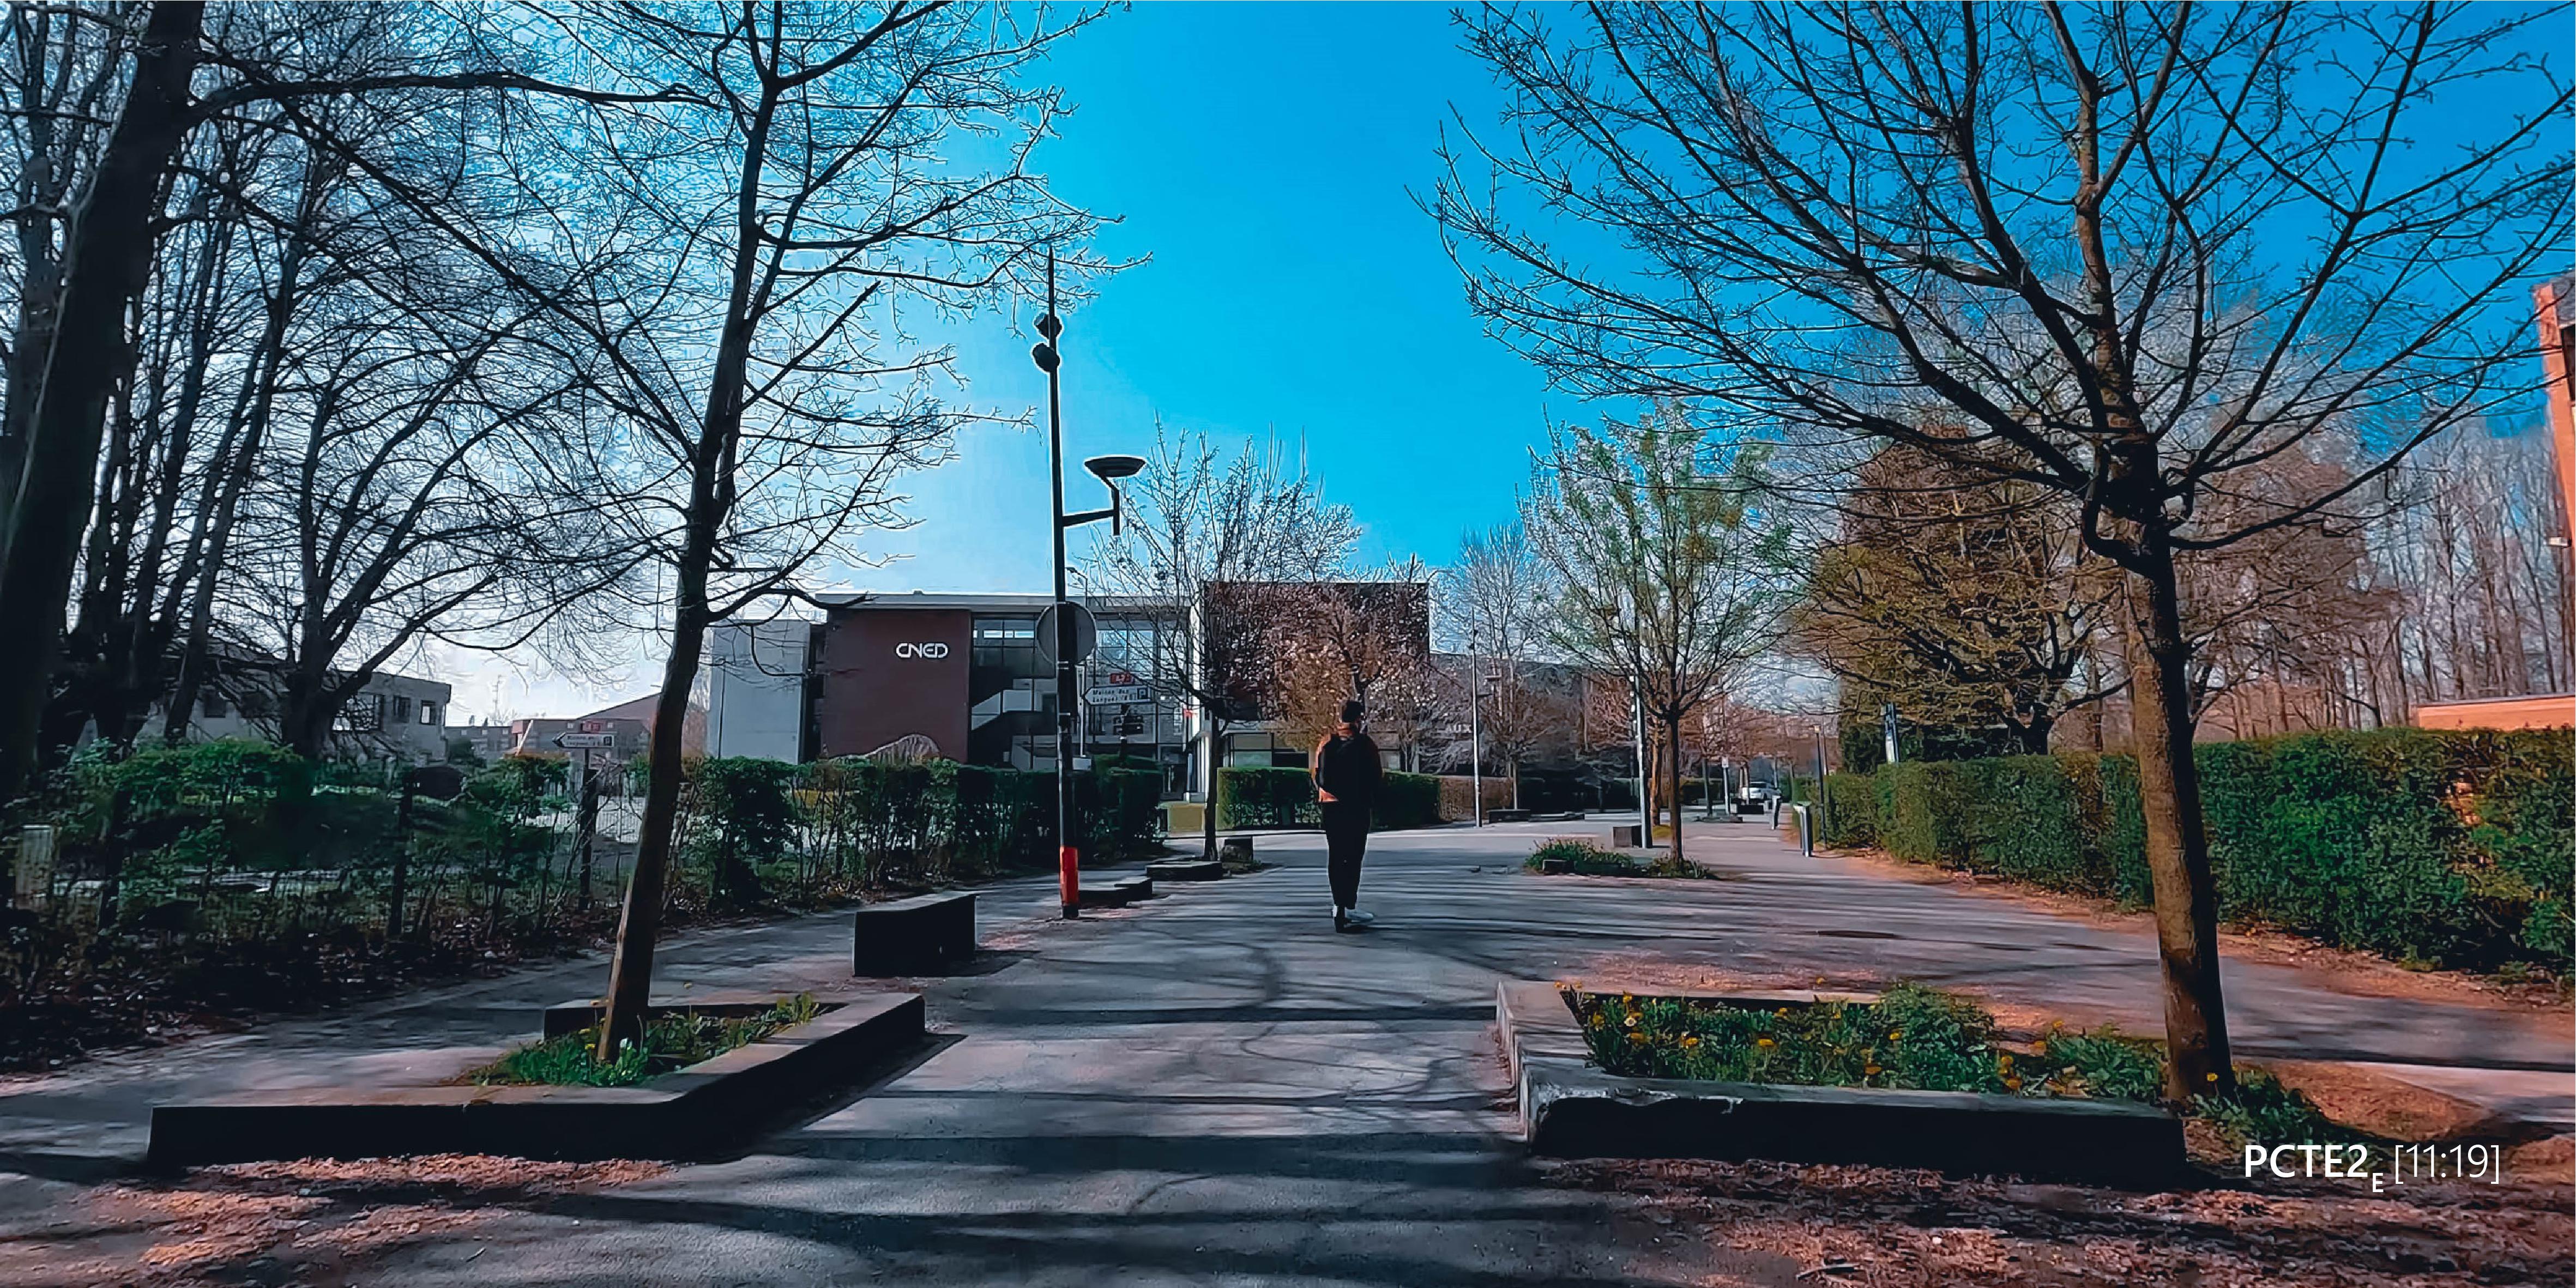
\includegraphics[width=0.75\columnwidth]{src/Figures/Annexes/Extrait_Video_PCTE2_Egress_9.jpg}}
        \vspace{5pt}
        \begin{flushright}\scriptsize{
        Author: \textcolor{blue}{Dylan Moinse (2022)}
        }\end{flushright}
    \end{figure}